\documentclass[twoside]{book}

% Packages required by doxygen
\usepackage{calc}
\usepackage{doxygen}
\usepackage{graphicx}
\usepackage[utf8]{inputenc}
\usepackage{makeidx}
\usepackage{multicol}
\usepackage{multirow}
\usepackage{textcomp}
\usepackage[table]{xcolor}

% NLS support packages
\usepackage[T2A]{fontenc}
\usepackage[russian]{babel}

% Font selection
\usepackage[T1]{fontenc}
\usepackage{mathptmx}
\usepackage[scaled=.90]{helvet}
\usepackage{courier}
\usepackage{amssymb}
\usepackage{sectsty}
\renewcommand{\familydefault}{\sfdefault}
\allsectionsfont{%
  \fontseries{bc}\selectfont%
  \color{darkgray}%
}
\renewcommand{\DoxyLabelFont}{%
  \fontseries{bc}\selectfont%
  \color{darkgray}%
}

% Page & text layout
\usepackage{geometry}
\geometry{%
  a4paper,%
  top=2.5cm,%
  bottom=2.5cm,%
  left=2.5cm,%
  right=2.5cm%
}
\tolerance=750
\hfuzz=15pt
\hbadness=750
\setlength{\emergencystretch}{15pt}
\setlength{\parindent}{0cm}
\setlength{\parskip}{0.2cm}
\makeatletter
\renewcommand{\paragraph}{%
  \@startsection{paragraph}{4}{0ex}{-1.0ex}{1.0ex}{%
    \normalfont\normalsize\bfseries\SS@parafont%
  }%
}
\renewcommand{\subparagraph}{%
  \@startsection{subparagraph}{5}{0ex}{-1.0ex}{1.0ex}{%
    \normalfont\normalsize\bfseries\SS@subparafont%
  }%
}
\makeatother

% Headers & footers
\usepackage{fancyhdr}
\pagestyle{fancyplain}
\fancyhead[LE]{\fancyplain{}{\bfseries\thepage}}
\fancyhead[CE]{\fancyplain{}{}}
\fancyhead[RE]{\fancyplain{}{\bfseries\leftmark}}
\fancyhead[LO]{\fancyplain{}{\bfseries\rightmark}}
\fancyhead[CO]{\fancyplain{}{}}
\fancyhead[RO]{\fancyplain{}{\bfseries\thepage}}
\fancyfoot[LE]{\fancyplain{}{}}
\fancyfoot[CE]{\fancyplain{}{}}
\fancyfoot[RE]{\fancyplain{}{\bfseries\scriptsize Документация по КМС2. Последние изменения\-: Чт 20 Окт 2016 11\-:06\-:14. Создано системой Doxygen }}
\fancyfoot[LO]{\fancyplain{}{\bfseries\scriptsize Документация по КМС2. Последние изменения\-: Чт 20 Окт 2016 11\-:06\-:14. Создано системой Doxygen }}
\fancyfoot[CO]{\fancyplain{}{}}
\fancyfoot[RO]{\fancyplain{}{}}
\renewcommand{\footrulewidth}{0.4pt}
\renewcommand{\chaptermark}[1]{%
  \markboth{#1}{}%
}
\renewcommand{\sectionmark}[1]{%
  \markright{\thesection\ #1}%
}

% Indices & bibliography
\usepackage{natbib}
\usepackage[titles]{tocloft}
\setcounter{tocdepth}{3}
\setcounter{secnumdepth}{5}
\makeindex

% Hyperlinks (required, but should be loaded last)
\usepackage{ifpdf}
\ifpdf
  \usepackage[pdftex,pagebackref=true]{hyperref}
\else
  \usepackage[ps2pdf,pagebackref=true]{hyperref}
\fi
\hypersetup{%
  colorlinks=true,%
  linkcolor=blue,%
  citecolor=blue,%
  unicode%
}

% Custom commands
\newcommand{\clearemptydoublepage}{%
  \newpage{\pagestyle{empty}\cleardoublepage}%
}


%===== C O N T E N T S =====

\begin{document}

% Titlepage & ToC
\hypersetup{pageanchor=false}
\pagenumbering{roman}
\begin{titlepage}
\vspace*{7cm}
\begin{center}%
{\Large КМС2 }\\
\vspace*{1cm}
{\large Создано системой Doxygen 1.8.6}\\
\vspace*{0.5cm}
{\small Чт 20 Окт 2016 11:06:14}\\
\end{center}
\end{titlepage}
\clearemptydoublepage
\tableofcontents
\clearemptydoublepage
\pagenumbering{arabic}
\hypersetup{pageanchor=true}

%--- Begin generated contents ---
\chapter{Алфавитный указатель пространств имен}
\section{Пространства имен}
Полный список пространств имен.\begin{DoxyCompactList}
\item\contentsline{section}{\hyperlink{namespaceLIBKMS__namespace}{L\-I\-B\-K\-M\-S\-\_\-namespace} }{\pageref{namespaceLIBKMS__namespace}}{}
\item\contentsline{section}{\hyperlink{namespaceLIBKMS__namespace_1_1exception}{L\-I\-B\-K\-M\-S\-\_\-namespace\-::exception} }{\pageref{namespaceLIBKMS__namespace_1_1exception}}{}
\item\contentsline{section}{\hyperlink{namespaceLIBKMS__namespace_1_1holder__util}{L\-I\-B\-K\-M\-S\-\_\-namespace\-::holder\-\_\-util} }{\pageref{namespaceLIBKMS__namespace_1_1holder__util}}{}
\item\contentsline{section}{\hyperlink{namespaceLIBKMS__namespace_1_1map__tools}{L\-I\-B\-K\-M\-S\-\_\-namespace\-::map\-\_\-tools} }{\pageref{namespaceLIBKMS__namespace_1_1map__tools}}{}
\item\contentsline{section}{\hyperlink{namespaceLIBKMS__namespace_1_1types}{L\-I\-B\-K\-M\-S\-\_\-namespace\-::types} }{\pageref{namespaceLIBKMS__namespace_1_1types}}{}
\item\contentsline{section}{\hyperlink{namespaceLIBKMS__namespace_1_1util}{L\-I\-B\-K\-M\-S\-\_\-namespace\-::util} }{\pageref{namespaceLIBKMS__namespace_1_1util}}{}
\end{DoxyCompactList}

\chapter{Иерархический список классов}
\section{Иерархия классов}
Иерархия классов.\begin{DoxyCompactList}
\item bad\-\_\-cast\begin{DoxyCompactList}
\item \contentsline{section}{L\-I\-B\-K\-M\-S\-\_\-namespace\-:\-:exception\-:\-:invalid\-\_\-type}{\pageref{classLIBKMS__namespace_1_1exception_1_1invalid__type}}{}
\end{DoxyCompactList}
\item \contentsline{section}{L\-I\-B\-K\-M\-S\-\_\-namespace\-:\-:Block\-Class\-Factory$<$ Function\-Storage, Subprogram, Subprogram\-Ptr, Block\-Ptr, Bl\-Cl\-Spec $>$\-:\-:block\-\_\-class\-\_\-with\-\_\-config$<$ T $>$}{\pageref{structLIBKMS__namespace_1_1BlockClassFactory_1_1block__class__with__config}}{}
\item \contentsline{section}{L\-I\-B\-K\-M\-S\-\_\-namespace\-:\-:Block\-Class$<$ Function\-Storage, Subprogram, Subprogram\-Ptr, Block\-Ptr, Bl\-Cl\-Spec $>$}{\pageref{classLIBKMS__namespace_1_1BlockClass}}{}
\begin{DoxyCompactList}
\item \contentsline{section}{L\-I\-B\-K\-M\-S\-\_\-namespace\-:\-:Block\-Class\-With\-Config$<$ Function\-Storage, Subprogram, Subprogram\-Ptr, Block\-Ptr, Config\-Node, Bl\-Cl\-Spec $>$}{\pageref{structLIBKMS__namespace_1_1BlockClassWithConfig}}{}
\end{DoxyCompactList}
\item \contentsline{section}{L\-I\-B\-K\-M\-S\-\_\-namespace\-:\-:Block\-Class\-Factory$<$ Function\-Storage, Subprogram, Subprogram\-Ptr, Block\-Ptr, Bl\-Cl\-Spec $>$}{\pageref{classLIBKMS__namespace_1_1BlockClassFactory}}{}
\item \contentsline{section}{L\-I\-B\-K\-M\-S\-\_\-namespace\-:\-:Callable$<$ Logger, Parameter\-Map, Formula\-Solver $>$}{\pageref{classLIBKMS__namespace_1_1Callable}}{}
\begin{DoxyCompactList}
\item \contentsline{section}{L\-I\-B\-K\-M\-S\-\_\-namespace\-:\-:Subprogram$<$ Logger, Parameter\-Map, Formula\-Solver $>$}{\pageref{classLIBKMS__namespace_1_1Subprogram}}{}
\end{DoxyCompactList}
\item \contentsline{section}{L\-I\-B\-K\-M\-S\-\_\-namespace\-:\-:Callable$<$ Logger, Param\-Spec$<$ Type\-Factory\-:\-:parameter\-\_\-t $>$\-:\-:map, Formula\-Solver $>$}{\pageref{classLIBKMS__namespace_1_1Callable}}{}
\begin{DoxyCompactList}
\item \contentsline{section}{L\-I\-B\-K\-M\-S\-\_\-namespace\-:\-:Block$<$ Type\-Factory, Param\-Spec, Scheduler, Logger, Subpr\-Spec, String\-Spec, Bl\-Cl\-Spec, Formula\-Solver $>$}{\pageref{classLIBKMS__namespace_1_1Block}}{}
\end{DoxyCompactList}
\item \contentsline{section}{L\-I\-B\-K\-M\-S\-\_\-namespace\-:\-:class\-\_\-spec$<$ Param\-Ext, Param\-Spec, Scheduler, Logger, Subpr\-Spec, String\-Spec, Block\-Class\-Spec, Power\-On\-Formula\-Solver $>$}{\pageref{structLIBKMS__namespace_1_1class__spec}}{}
\item \contentsline{section}{L\-I\-B\-K\-M\-S\-\_\-namespace\-:\-:Control\-Func$<$ Type\-Factory, Block\-Ptr, Logger $>$}{\pageref{classLIBKMS__namespace_1_1ControlFunc}}{}
\item \contentsline{section}{L\-I\-B\-K\-M\-S\-\_\-namespace\-:\-:Control\-Func\-Storage$<$ Type\-Factory, Block\-Ptr, Logger, Spec $>$}{\pageref{classLIBKMS__namespace_1_1ControlFuncStorage}}{}
\item exception\begin{DoxyCompactList}
\item \contentsline{section}{L\-I\-B\-K\-M\-S\-\_\-namespace\-:\-:Subprogram$<$ Logger, Parameter\-Map, Formula\-Solver $>$\-:\-:user\-\_\-exception}{\pageref{structLIBKMS__namespace_1_1Subprogram_1_1user__exception}}{}
\end{DoxyCompactList}
\item Ext\begin{DoxyCompactList}
\item \contentsline{section}{L\-I\-B\-K\-M\-S\-\_\-namespace\-:\-:Parameter$<$ Ext, Spec $>$}{\pageref{classLIBKMS__namespace_1_1Parameter}}{}
\begin{DoxyCompactList}
\item \contentsline{section}{L\-I\-B\-K\-M\-S\-\_\-namespace\-:\-:Holder$<$ T, Parameter $>$}{\pageref{classLIBKMS__namespace_1_1Holder}}{}
\end{DoxyCompactList}
\end{DoxyCompactList}
\item \contentsline{section}{L\-I\-B\-K\-M\-S\-\_\-namespace\-:\-:Function\-Storage$<$ Parameter\-Map $>$}{\pageref{classLIBKMS__namespace_1_1FunctionStorage}}{}
\item \contentsline{section}{L\-I\-B\-K\-M\-S\-\_\-namespace\-:\-:map\-\_\-tools\-:\-:get$<$ T $>$}{\pageref{structLIBKMS__namespace_1_1map__tools_1_1get}}{}
\item \contentsline{section}{L\-I\-B\-K\-M\-S\-\_\-namespace\-:\-:types\-:\-:get\-\_\-return\-\_\-type$<$ T, P $>$}{\pageref{structLIBKMS__namespace_1_1types_1_1get__return__type}}{}
\item \contentsline{section}{L\-I\-B\-K\-M\-S\-\_\-namespace\-:\-:types\-:\-:get\-\_\-return\-\_\-type$<$ std\-\_\-types\-:\-:t\-Bool, P $>$}{\pageref{structLIBKMS__namespace_1_1types_1_1get__return__type_3_01std__types_1_1tBool_00_01P_01_4}}{}
\item \contentsline{section}{L\-I\-B\-K\-M\-S\-\_\-namespace\-:\-:types\-:\-:get\-\_\-return\-\_\-type$<$ std\-\_\-types\-:\-:t\-Int, P $>$}{\pageref{structLIBKMS__namespace_1_1types_1_1get__return__type_3_01std__types_1_1tInt_00_01P_01_4}}{}
\item \contentsline{section}{L\-I\-B\-K\-M\-S\-\_\-namespace\-:\-:types\-:\-:get\-\_\-return\-\_\-type$<$ std\-\_\-types\-:\-:t\-Real, P $>$}{\pageref{structLIBKMS__namespace_1_1types_1_1get__return__type_3_01std__types_1_1tReal_00_01P_01_4}}{}
\item \contentsline{section}{L\-I\-B\-K\-M\-S\-\_\-namespace\-:\-:types\-:\-:get\-\_\-return\-\_\-type$<$ std\-\_\-types\-:\-:t\-String, P $>$}{\pageref{structLIBKMS__namespace_1_1types_1_1get__return__type_3_01std__types_1_1tString_00_01P_01_4}}{}
\item \contentsline{section}{L\-I\-B\-K\-M\-S\-\_\-namespace\-:\-:class\-\_\-spec$<$ Param\-Ext, Param\-Spec, Scheduler, Logger, Subpr\-Spec, String\-Spec, Block\-Class\-Spec, Power\-On\-Formula\-Solver $>$\-:\-:holder$<$ T $>$}{\pageref{structLIBKMS__namespace_1_1class__spec_1_1holder}}{}
\item \contentsline{section}{L\-I\-B\-K\-M\-S\-\_\-namespace\-:\-:obj\-\_\-as$<$ Holder$<$ T, P $>$, P $>$}{\pageref{structLIBKMS__namespace_1_1obj__as_3_01Holder_3_01T_00_01P_01_4_00_01P_01_4}}{}
\item out\-\_\-of\-\_\-range\begin{DoxyCompactList}
\item \contentsline{section}{L\-I\-B\-K\-M\-S\-\_\-namespace\-:\-:exception\-:\-:invalid\-\_\-var\-\_\-name}{\pageref{classLIBKMS__namespace_1_1exception_1_1invalid__var__name}}{}
\end{DoxyCompactList}
\item \contentsline{section}{L\-I\-B\-K\-M\-S\-\_\-namespace\-:\-:Type\-Factory$<$ Ext, Spec $>$}{\pageref{classLIBKMS__namespace_1_1TypeFactory}}{}
\end{DoxyCompactList}

\chapter{Алфавитный указатель классов}
\section{Классы}
Классы с их кратким описанием.\begin{DoxyCompactList}
\item\contentsline{section}{\hyperlink{classLIBKMS__namespace_1_1Block}{L\-I\-B\-K\-M\-S\-\_\-namespace\-::\-Block$<$ Type\-Factory, Param\-Spec, Scheduler, Logger, Subpr\-Spec, String\-Spec, Bl\-Cl\-Spec, Formula\-Solver $>$} \\*Шаблонный класс \hyperlink{classLIBKMS__namespace_1_1Block}{Block}, отображающий блок процесс }{\pageref{classLIBKMS__namespace_1_1Block}}{}
\item\contentsline{section}{\hyperlink{structLIBKMS__namespace_1_1BlockClassFactory_1_1block__class__with__config}{L\-I\-B\-K\-M\-S\-\_\-namespace\-::\-Block\-Class\-Factory$<$ Function\-Storage, Subprogram, Subprogram\-Ptr, Block\-Ptr, Bl\-Cl\-Spec $>$\-::block\-\_\-class\-\_\-with\-\_\-config$<$ T $>$} }{\pageref{structLIBKMS__namespace_1_1BlockClassFactory_1_1block__class__with__config}}{}
\item\contentsline{section}{\hyperlink{classLIBKMS__namespace_1_1BlockClass}{L\-I\-B\-K\-M\-S\-\_\-namespace\-::\-Block\-Class$<$ Function\-Storage, Subprogram, Subprogram\-Ptr, Block\-Ptr, Bl\-Cl\-Spec $>$} \\*Прототип описания класса блока }{\pageref{classLIBKMS__namespace_1_1BlockClass}}{}
\item\contentsline{section}{\hyperlink{classLIBKMS__namespace_1_1BlockClassFactory}{L\-I\-B\-K\-M\-S\-\_\-namespace\-::\-Block\-Class\-Factory$<$ Function\-Storage, Subprogram, Subprogram\-Ptr, Block\-Ptr, Bl\-Cl\-Spec $>$} \\*Фабрика классов блоков }{\pageref{classLIBKMS__namespace_1_1BlockClassFactory}}{}
\item\contentsline{section}{\hyperlink{structLIBKMS__namespace_1_1BlockClassWithConfig}{L\-I\-B\-K\-M\-S\-\_\-namespace\-::\-Block\-Class\-With\-Config$<$ Function\-Storage, Subprogram, Subprogram\-Ptr, Block\-Ptr, Config\-Node, Bl\-Cl\-Spec $>$} }{\pageref{structLIBKMS__namespace_1_1BlockClassWithConfig}}{}
\item\contentsline{section}{\hyperlink{classLIBKMS__namespace_1_1Callable}{L\-I\-B\-K\-M\-S\-\_\-namespace\-::\-Callable$<$ Logger, Parameter\-Map, Formula\-Solver $>$} }{\pageref{classLIBKMS__namespace_1_1Callable}}{}
\item\contentsline{section}{\hyperlink{structLIBKMS__namespace_1_1class__spec}{L\-I\-B\-K\-M\-S\-\_\-namespace\-::class\-\_\-spec$<$ Param\-Ext, Param\-Spec, Scheduler, Logger, Subpr\-Spec, String\-Spec, Block\-Class\-Spec, Power\-On\-Formula\-Solver $>$} }{\pageref{structLIBKMS__namespace_1_1class__spec}}{}
\item\contentsline{section}{\hyperlink{classLIBKMS__namespace_1_1ControlFunc}{L\-I\-B\-K\-M\-S\-\_\-namespace\-::\-Control\-Func$<$ Type\-Factory, Block\-Ptr, Logger $>$} \\*Шаблон класса \char`\"{}управляющая функция\char`\"{} (ФИ) }{\pageref{classLIBKMS__namespace_1_1ControlFunc}}{}
\item\contentsline{section}{\hyperlink{classLIBKMS__namespace_1_1ControlFuncStorage}{L\-I\-B\-K\-M\-S\-\_\-namespace\-::\-Control\-Func\-Storage$<$ Type\-Factory, Block\-Ptr, Logger, Spec $>$} }{\pageref{classLIBKMS__namespace_1_1ControlFuncStorage}}{}
\item\contentsline{section}{\hyperlink{classLIBKMS__namespace_1_1FunctionStorage}{L\-I\-B\-K\-M\-S\-\_\-namespace\-::\-Function\-Storage$<$ Parameter\-Map $>$} \\*Фабрика подпрограмм }{\pageref{classLIBKMS__namespace_1_1FunctionStorage}}{}
\item\contentsline{section}{\hyperlink{structLIBKMS__namespace_1_1map__tools_1_1get}{L\-I\-B\-K\-M\-S\-\_\-namespace\-::map\-\_\-tools\-::get$<$ T $>$} \\*Извлечь параметр определенного типа из шаблона }{\pageref{structLIBKMS__namespace_1_1map__tools_1_1get}}{}
\item\contentsline{section}{\hyperlink{structLIBKMS__namespace_1_1types_1_1get__return__type}{L\-I\-B\-K\-M\-S\-\_\-namespace\-::types\-::get\-\_\-return\-\_\-type$<$ T, P $>$} \\*Для осуществления возможности возврата holder$<$ T $>$ по T }{\pageref{structLIBKMS__namespace_1_1types_1_1get__return__type}}{}
\item\contentsline{section}{\hyperlink{structLIBKMS__namespace_1_1types_1_1get__return__type_3_01std__types_1_1tBool_00_01P_01_4}{L\-I\-B\-K\-M\-S\-\_\-namespace\-::types\-::get\-\_\-return\-\_\-type$<$ std\-\_\-types\-::t\-Bool, P $>$} }{\pageref{structLIBKMS__namespace_1_1types_1_1get__return__type_3_01std__types_1_1tBool_00_01P_01_4}}{}
\item\contentsline{section}{\hyperlink{structLIBKMS__namespace_1_1types_1_1get__return__type_3_01std__types_1_1tInt_00_01P_01_4}{L\-I\-B\-K\-M\-S\-\_\-namespace\-::types\-::get\-\_\-return\-\_\-type$<$ std\-\_\-types\-::t\-Int, P $>$} }{\pageref{structLIBKMS__namespace_1_1types_1_1get__return__type_3_01std__types_1_1tInt_00_01P_01_4}}{}
\item\contentsline{section}{\hyperlink{structLIBKMS__namespace_1_1types_1_1get__return__type_3_01std__types_1_1tReal_00_01P_01_4}{L\-I\-B\-K\-M\-S\-\_\-namespace\-::types\-::get\-\_\-return\-\_\-type$<$ std\-\_\-types\-::t\-Real, P $>$} }{\pageref{structLIBKMS__namespace_1_1types_1_1get__return__type_3_01std__types_1_1tReal_00_01P_01_4}}{}
\item\contentsline{section}{\hyperlink{structLIBKMS__namespace_1_1types_1_1get__return__type_3_01std__types_1_1tString_00_01P_01_4}{L\-I\-B\-K\-M\-S\-\_\-namespace\-::types\-::get\-\_\-return\-\_\-type$<$ std\-\_\-types\-::t\-String, P $>$} }{\pageref{structLIBKMS__namespace_1_1types_1_1get__return__type_3_01std__types_1_1tString_00_01P_01_4}}{}
\item\contentsline{section}{\hyperlink{structLIBKMS__namespace_1_1class__spec_1_1holder}{L\-I\-B\-K\-M\-S\-\_\-namespace\-::class\-\_\-spec$<$ Param\-Ext, Param\-Spec, Scheduler, Logger, Subpr\-Spec, String\-Spec, Block\-Class\-Spec, Power\-On\-Formula\-Solver $>$\-::holder$<$ T $>$} }{\pageref{structLIBKMS__namespace_1_1class__spec_1_1holder}}{}
\item\contentsline{section}{\hyperlink{classLIBKMS__namespace_1_1Holder}{L\-I\-B\-K\-M\-S\-\_\-namespace\-::\-Holder$<$ T, Parameter $>$} \\*Класс-\/контейнер для стандартных типов }{\pageref{classLIBKMS__namespace_1_1Holder}}{}
\item\contentsline{section}{\hyperlink{classLIBKMS__namespace_1_1exception_1_1invalid__type}{L\-I\-B\-K\-M\-S\-\_\-namespace\-::exception\-::invalid\-\_\-type} }{\pageref{classLIBKMS__namespace_1_1exception_1_1invalid__type}}{}
\item\contentsline{section}{\hyperlink{classLIBKMS__namespace_1_1exception_1_1invalid__var__name}{L\-I\-B\-K\-M\-S\-\_\-namespace\-::exception\-::invalid\-\_\-var\-\_\-name} }{\pageref{classLIBKMS__namespace_1_1exception_1_1invalid__var__name}}{}
\item\contentsline{section}{\hyperlink{structLIBKMS__namespace_1_1obj__as_3_01Holder_3_01T_00_01P_01_4_00_01P_01_4}{L\-I\-B\-K\-M\-S\-\_\-namespace\-::obj\-\_\-as$<$ Holder$<$ T, P $>$, P $>$} \\*Специализация для преобразования parameter в Holder$<$ T $>$ }{\pageref{structLIBKMS__namespace_1_1obj__as_3_01Holder_3_01T_00_01P_01_4_00_01P_01_4}}{}
\item\contentsline{section}{\hyperlink{classLIBKMS__namespace_1_1Parameter}{L\-I\-B\-K\-M\-S\-\_\-namespace\-::\-Parameter$<$ Ext, Spec $>$} \\*Класс, от которого должны наследоваться все классы параметров }{\pageref{classLIBKMS__namespace_1_1Parameter}}{}
\item\contentsline{section}{\hyperlink{classLIBKMS__namespace_1_1Subprogram}{L\-I\-B\-K\-M\-S\-\_\-namespace\-::\-Subprogram$<$ Logger, Parameter\-Map, Formula\-Solver $>$} \\*Шаблонный класс -\/ обертка подпрограмм }{\pageref{classLIBKMS__namespace_1_1Subprogram}}{}
\item\contentsline{section}{\hyperlink{classLIBKMS__namespace_1_1TypeFactory}{L\-I\-B\-K\-M\-S\-\_\-namespace\-::\-Type\-Factory$<$ Ext, Spec $>$} \\*Фабрика параметров }{\pageref{classLIBKMS__namespace_1_1TypeFactory}}{}
\item\contentsline{section}{\hyperlink{structLIBKMS__namespace_1_1Subprogram_1_1user__exception}{L\-I\-B\-K\-M\-S\-\_\-namespace\-::\-Subprogram$<$ Logger, Parameter\-Map, Formula\-Solver $>$\-::user\-\_\-exception} }{\pageref{structLIBKMS__namespace_1_1Subprogram_1_1user__exception}}{}
\end{DoxyCompactList}

\chapter{Список файлов}
\section{Файлы}
Полный список файлов.\begin{DoxyCompactList}
\item\contentsline{section}{\hyperlink{block_8hpp}{block.\-hpp} }{\pageref{block_8hpp}}{}
\item\contentsline{section}{\hyperlink{block__class_8hpp}{block\-\_\-class.\-hpp} }{\pageref{block__class_8hpp}}{}
\item\contentsline{section}{\hyperlink{callable_8hpp}{callable.\-hpp} }{\pageref{callable_8hpp}}{}
\item\contentsline{section}{\hyperlink{class__spec_8hpp}{class\-\_\-spec.\-hpp} }{\pageref{class__spec_8hpp}}{}
\item\contentsline{section}{\hyperlink{control__func_8hpp}{control\-\_\-func.\-hpp} }{\pageref{control__func_8hpp}}{}
\item\contentsline{section}{\hyperlink{function__storage_8hpp}{function\-\_\-storage.\-hpp} }{\pageref{function__storage_8hpp}}{}
\item\contentsline{section}{\hyperlink{holder_8hpp}{holder.\-hpp} }{\pageref{holder_8hpp}}{}
\item\contentsline{section}{\hyperlink{kernel_8hpp}{kernel.\-hpp} }{\pageref{kernel_8hpp}}{}
\item\contentsline{section}{\hyperlink{param_8hpp}{param.\-hpp} }{\pageref{param_8hpp}}{}
\item\contentsline{section}{\hyperlink{subprog_8hpp}{subprog.\-hpp} }{\pageref{subprog_8hpp}}{}
\item\contentsline{section}{\hyperlink{typefactory_8hpp}{typefactory.\-hpp} }{\pageref{typefactory_8hpp}}{}
\end{DoxyCompactList}

\chapter{Пространства имен}
\hypertarget{namespaceLIBKMS__namespace}{\section{Пространство имен L\-I\-B\-K\-M\-S\-\_\-namespace}
\label{namespaceLIBKMS__namespace}\index{L\-I\-B\-K\-M\-S\-\_\-namespace@{L\-I\-B\-K\-M\-S\-\_\-namespace}}
}
\subsection*{Пространства имен}
\begin{DoxyCompactItemize}
\item 
\hyperlink{namespaceLIBKMS__namespace_1_1exception}{exception}
\item 
\hyperlink{namespaceLIBKMS__namespace_1_1holder__util}{holder\-\_\-util}
\item 
\hyperlink{namespaceLIBKMS__namespace_1_1map__tools}{map\-\_\-tools}
\item 
\hyperlink{namespaceLIBKMS__namespace_1_1types}{types}
\item 
\hyperlink{namespaceLIBKMS__namespace_1_1util}{util}
\end{DoxyCompactItemize}
\subsection*{Классы}
\begin{DoxyCompactItemize}
\item 
class \hyperlink{classLIBKMS__namespace_1_1Block}{Block}
\begin{DoxyCompactList}\small\item\em Шаблонный класс \hyperlink{classLIBKMS__namespace_1_1Block}{Block}, отображающий блок процесс. \end{DoxyCompactList}\item 
class \hyperlink{classLIBKMS__namespace_1_1BlockClass}{Block\-Class}
\begin{DoxyCompactList}\small\item\em Прототип описания класса блока \end{DoxyCompactList}\item 
struct \hyperlink{structLIBKMS__namespace_1_1BlockClassWithConfig}{Block\-Class\-With\-Config}
\item 
class \hyperlink{classLIBKMS__namespace_1_1BlockClassFactory}{Block\-Class\-Factory}
\begin{DoxyCompactList}\small\item\em Фабрика классов блоков \end{DoxyCompactList}\item 
class \hyperlink{classLIBKMS__namespace_1_1Callable}{Callable}
\item 
struct \hyperlink{structLIBKMS__namespace_1_1class__spec}{class\-\_\-spec}
\item 
class \hyperlink{classLIBKMS__namespace_1_1ControlFunc}{Control\-Func}
\begin{DoxyCompactList}\small\item\em Шаблон класса \char`\"{}управляющая функция\char`\"{} (ФИ) \end{DoxyCompactList}\item 
class \hyperlink{classLIBKMS__namespace_1_1ControlFuncStorage}{Control\-Func\-Storage}
\item 
class \hyperlink{classLIBKMS__namespace_1_1FunctionStorage}{Function\-Storage}
\begin{DoxyCompactList}\small\item\em Фабрика подпрограмм \end{DoxyCompactList}\item 
struct \hyperlink{structLIBKMS__namespace_1_1obj__as_3_01Holder_3_01T_00_01P_01_4_00_01P_01_4}{obj\-\_\-as$<$ Holder$<$ T, P $>$, P $>$}
\begin{DoxyCompactList}\small\item\em Специализация для преобразования parameter в Holder$<$ T $>$ \end{DoxyCompactList}\item 
class \hyperlink{classLIBKMS__namespace_1_1Holder}{Holder}
\begin{DoxyCompactList}\small\item\em Класс-\/контейнер для стандартных типов \end{DoxyCompactList}\item 
class \hyperlink{classLIBKMS__namespace_1_1Parameter}{Parameter}
\begin{DoxyCompactList}\small\item\em Класс, от которого должны наследоваться все классы параметров \end{DoxyCompactList}\item 
class \hyperlink{classLIBKMS__namespace_1_1Subprogram}{Subprogram}
\begin{DoxyCompactList}\small\item\em Шаблонный класс -\/ обертка подпрограмм \end{DoxyCompactList}\item 
class \hyperlink{classLIBKMS__namespace_1_1TypeFactory}{Type\-Factory}
\begin{DoxyCompactList}\small\item\em Фабрика параметров \end{DoxyCompactList}\end{DoxyCompactItemize}
\subsection*{Определения типов}
\begin{DoxyCompactItemize}
\item 
typedef \hyperlink{structLIBKMS__namespace_1_1class__spec}{class\-\_\-spec}\\*
$<$ No\-Extension, \\*
remappable\-\_\-shared\-\_\-ptr\-\_\-spec, \\*
Std\-Scheduler$<$ Std\-Logger $>$\\*
, Std\-Logger, shared\-\_\-ptr\-\_\-spec, \\*
Std\-String\-Spec, shared\-\_\-ptr\-\_\-spec, \\*
Std\-Power\-On\-Formula\-Solver $>$ \hyperlink{namespaceLIBKMS__namespace_ae7952b6893ea0986997f67d2945fc1a1}{std\-\_\-class\-\_\-spec}
\begin{DoxyCompactList}\small\item\em Стандартная специализация для шаблона \end{DoxyCompactList}\end{DoxyCompactItemize}


\subsection{Типы}
\hypertarget{namespaceLIBKMS__namespace_ae7952b6893ea0986997f67d2945fc1a1}{\index{L\-I\-B\-K\-M\-S\-\_\-namespace@{L\-I\-B\-K\-M\-S\-\_\-namespace}!std\-\_\-class\-\_\-spec@{std\-\_\-class\-\_\-spec}}
\index{std\-\_\-class\-\_\-spec@{std\-\_\-class\-\_\-spec}!LIBKMS_namespace@{L\-I\-B\-K\-M\-S\-\_\-namespace}}
\subsubsection[{std\-\_\-class\-\_\-spec}]{\setlength{\rightskip}{0pt plus 5cm}typedef {\bf class\-\_\-spec}$<$ No\-Extension, remappable\-\_\-shared\-\_\-ptr\-\_\-spec, Std\-Scheduler$<$ Std\-Logger $>$, Std\-Logger, shared\-\_\-ptr\-\_\-spec, Std\-String\-Spec, shared\-\_\-ptr\-\_\-spec, Std\-Power\-On\-Formula\-Solver $>$ {\bf L\-I\-B\-K\-M\-S\-\_\-namespace\-::std\-\_\-class\-\_\-spec}}}\label{namespaceLIBKMS__namespace_ae7952b6893ea0986997f67d2945fc1a1}


Стандартная специализация для шаблона 


\hypertarget{namespaceLIBKMS__namespace_1_1exception}{\section{Пространство имен L\-I\-B\-K\-M\-S\-\_\-namespace\-:\-:exception}
\label{namespaceLIBKMS__namespace_1_1exception}\index{L\-I\-B\-K\-M\-S\-\_\-namespace\-::exception@{L\-I\-B\-K\-M\-S\-\_\-namespace\-::exception}}
}
\subsection*{Классы}
\begin{DoxyCompactItemize}
\item 
class \hyperlink{classLIBKMS__namespace_1_1exception_1_1invalid__var__name}{invalid\-\_\-var\-\_\-name}
\item 
class \hyperlink{classLIBKMS__namespace_1_1exception_1_1invalid__type}{invalid\-\_\-type}
\end{DoxyCompactItemize}

\hypertarget{namespaceLIBKMS__namespace_1_1holder__util}{\section{Пространство имен L\-I\-B\-K\-M\-S\-\_\-namespace\-:\-:holder\-\_\-util}
\label{namespaceLIBKMS__namespace_1_1holder__util}\index{L\-I\-B\-K\-M\-S\-\_\-namespace\-::holder\-\_\-util@{L\-I\-B\-K\-M\-S\-\_\-namespace\-::holder\-\_\-util}}
}
\subsection*{Функции}
\begin{DoxyCompactItemize}
\item 
{\footnotesize template$<$typename T $>$ }\\std\-::string \hyperlink{namespaceLIBKMS__namespace_1_1holder__util_a3f905fcf57ce738c4f3a82676d0cf590}{to\-\_\-string} (const T \&m)
\begin{DoxyCompactList}\small\item\em Шаблон функции для печати данных в строку \end{DoxyCompactList}\item 
{\footnotesize template$<$typename T $>$ }\\bool \hyperlink{namespaceLIBKMS__namespace_1_1holder__util_a0d969ce1aeb62ef97c3a280cfb000b31}{from\-\_\-string} (const std\-::string \&src, T \&dst)
\begin{DoxyCompactList}\small\item\em Шаблон функции для извлечения данных из строки \end{DoxyCompactList}\item 
{\footnotesize template$<$typename T $>$ }\\std\-::vector$<$ uint8\-\_\-t $>$ \hyperlink{namespaceLIBKMS__namespace_1_1holder__util_a80baff5a69342a580b476e44ee03fdbd}{to\-\_\-bytes} (const T \&src)
\begin{DoxyCompactList}\small\item\em Шаблон функции для представления данных в виде вектора байтов \end{DoxyCompactList}\item 
{\footnotesize template$<$typename T $>$ }\\bool \hyperlink{namespaceLIBKMS__namespace_1_1holder__util_a6b44331a32e5c812376a11812c500941}{from\-\_\-bytes} (const uint8\-\_\-t $\ast$src, size\-\_\-t len, T \&dst)
\begin{DoxyCompactList}\small\item\em Шаблон функции для извлечения данных из набора байтов \end{DoxyCompactList}\item 
{\footnotesize template$<$typename T $>$ }\\bool \hyperlink{namespaceLIBKMS__namespace_1_1holder__util_a7e56d3601efc7f34cdd9d4cfb699c100}{is\-\_\-set} (const T \&src)
\begin{DoxyCompactList}\small\item\em Шаблон функции для проверки установки значения \end{DoxyCompactList}\item 
{\footnotesize template$<$typename T $>$ }\\bool \hyperlink{namespaceLIBKMS__namespace_1_1holder__util_a38a7545f9c34955520ea5e09ecadd6de}{copy\-\_\-data} (T \&dst, T \&src)
\begin{DoxyCompactList}\small\item\em Шаблон для копирования данных \end{DoxyCompactList}\item 
{\footnotesize template$<$$>$ }\\std\-::string \hyperlink{namespaceLIBKMS__namespace_1_1holder__util_a3b09772362bd2dfcc6d8c815a2a17714}{to\-\_\-string} (const std\-\_\-types\-::t\-Bool \&d)
\item 
{\footnotesize template$<$$>$ }\\std\-::string \hyperlink{namespaceLIBKMS__namespace_1_1holder__util_adff56c8a003b35a1416ea79b5ffb96a1}{to\-\_\-string} (const std\-\_\-types\-::t\-Real \&d)
\item 
{\footnotesize template$<$$>$ }\\std\-::string \hyperlink{namespaceLIBKMS__namespace_1_1holder__util_a286232c0d65ab9d20250b6ad81049457}{to\-\_\-string} (const std\-\_\-types\-::t\-Int \&d)
\item 
{\footnotesize template$<$$>$ }\\std\-::string \hyperlink{namespaceLIBKMS__namespace_1_1holder__util_a6695a085005f1cd5c405c5bae944f580}{to\-\_\-string} (const std\-\_\-types\-::t\-String \&value)
\item 
{\footnotesize template$<$$>$ }\\bool \hyperlink{namespaceLIBKMS__namespace_1_1holder__util_a4b7a0123fb5a66cd39453c79b109afc8}{from\-\_\-string} (const std\-::string \&src, std\-\_\-types\-::t\-String \&dst)
\item 
{\footnotesize template$<$$>$ }\\bool \hyperlink{namespaceLIBKMS__namespace_1_1holder__util_a85eaede4657c0cbfc37731777afe0943}{from\-\_\-bytes} (const uint8\-\_\-t $\ast$src, size\-\_\-t len, std\-\_\-types\-::t\-Bool \&dst)
\item 
{\footnotesize template$<$$>$ }\\bool \hyperlink{namespaceLIBKMS__namespace_1_1holder__util_a77f67b68898531c2b8310bfb586d7b66}{from\-\_\-bytes} (const uint8\-\_\-t $\ast$src, size\-\_\-t len, std\-\_\-types\-::t\-String \&dst)
\item 
{\footnotesize template$<$$>$ }\\std\-::vector$<$ uint8\-\_\-t $>$ \hyperlink{namespaceLIBKMS__namespace_1_1holder__util_acc9c93112aca3eddfe3a05e26b9251b0}{to\-\_\-bytes} (const std\-\_\-types\-::t\-Bool \&src)
\item 
{\footnotesize template$<$$>$ }\\std\-::vector$<$ uint8\-\_\-t $>$ \hyperlink{namespaceLIBKMS__namespace_1_1holder__util_a082d59ec1281ddf638a49c61fd301c0e}{to\-\_\-bytes} (const std\-\_\-types\-::t\-Int \&src)
\item 
{\footnotesize template$<$$>$ }\\std\-::vector$<$ uint8\-\_\-t $>$ \hyperlink{namespaceLIBKMS__namespace_1_1holder__util_a97fe6e13277dd847fa4f31e1a88e89a7}{to\-\_\-bytes} (const std\-\_\-types\-::t\-Real \&src)
\item 
{\footnotesize template$<$$>$ }\\std\-::vector$<$ uint8\-\_\-t $>$ \hyperlink{namespaceLIBKMS__namespace_1_1holder__util_acdc1b01e2f4c4d6c9dcb62a29d04e7ea}{to\-\_\-bytes} (const std\-\_\-types\-::t\-String \&src)
\item 
{\footnotesize template$<$$>$ }\\bool \hyperlink{namespaceLIBKMS__namespace_1_1holder__util_a1d62c700f994ec71e92770ebbfa7da16}{is\-\_\-set} (const std\-\_\-types\-::t\-String \&src)
\end{DoxyCompactItemize}


\subsection{Функции}
\hypertarget{namespaceLIBKMS__namespace_1_1holder__util_a38a7545f9c34955520ea5e09ecadd6de}{\index{L\-I\-B\-K\-M\-S\-\_\-namespace\-::holder\-\_\-util@{L\-I\-B\-K\-M\-S\-\_\-namespace\-::holder\-\_\-util}!copy\-\_\-data@{copy\-\_\-data}}
\index{copy\-\_\-data@{copy\-\_\-data}!LIBKMS_namespace::holder_util@{L\-I\-B\-K\-M\-S\-\_\-namespace\-::holder\-\_\-util}}
\subsubsection[{copy\-\_\-data}]{\setlength{\rightskip}{0pt plus 5cm}template$<$typename T $>$ bool L\-I\-B\-K\-M\-S\-\_\-namespace\-::holder\-\_\-util\-::copy\-\_\-data (
\begin{DoxyParamCaption}
\item[{T \&}]{dst, }
\item[{T \&}]{src}
\end{DoxyParamCaption}
)\hspace{0.3cm}{\ttfamily [inline]}}}\label{namespaceLIBKMS__namespace_1_1holder__util_a38a7545f9c34955520ea5e09ecadd6de}


Шаблон для копирования данных 

\hypertarget{namespaceLIBKMS__namespace_1_1holder__util_a6b44331a32e5c812376a11812c500941}{\index{L\-I\-B\-K\-M\-S\-\_\-namespace\-::holder\-\_\-util@{L\-I\-B\-K\-M\-S\-\_\-namespace\-::holder\-\_\-util}!from\-\_\-bytes@{from\-\_\-bytes}}
\index{from\-\_\-bytes@{from\-\_\-bytes}!LIBKMS_namespace::holder_util@{L\-I\-B\-K\-M\-S\-\_\-namespace\-::holder\-\_\-util}}
\subsubsection[{from\-\_\-bytes}]{\setlength{\rightskip}{0pt plus 5cm}template$<$typename T $>$ bool L\-I\-B\-K\-M\-S\-\_\-namespace\-::holder\-\_\-util\-::from\-\_\-bytes (
\begin{DoxyParamCaption}
\item[{const uint8\-\_\-t $\ast$}]{src, }
\item[{size\-\_\-t}]{len, }
\item[{T \&}]{dst}
\end{DoxyParamCaption}
)\hspace{0.3cm}{\ttfamily [inline]}}}\label{namespaceLIBKMS__namespace_1_1holder__util_a6b44331a32e5c812376a11812c500941}


Шаблон функции для извлечения данных из набора байтов 

\hypertarget{namespaceLIBKMS__namespace_1_1holder__util_a85eaede4657c0cbfc37731777afe0943}{\index{L\-I\-B\-K\-M\-S\-\_\-namespace\-::holder\-\_\-util@{L\-I\-B\-K\-M\-S\-\_\-namespace\-::holder\-\_\-util}!from\-\_\-bytes@{from\-\_\-bytes}}
\index{from\-\_\-bytes@{from\-\_\-bytes}!LIBKMS_namespace::holder_util@{L\-I\-B\-K\-M\-S\-\_\-namespace\-::holder\-\_\-util}}
\subsubsection[{from\-\_\-bytes}]{\setlength{\rightskip}{0pt plus 5cm}template$<$$>$ bool L\-I\-B\-K\-M\-S\-\_\-namespace\-::holder\-\_\-util\-::from\-\_\-bytes (
\begin{DoxyParamCaption}
\item[{const uint8\-\_\-t $\ast$}]{src, }
\item[{size\-\_\-t}]{len, }
\item[{std\-\_\-types\-::t\-Bool \&}]{dst}
\end{DoxyParamCaption}
)\hspace{0.3cm}{\ttfamily [inline]}}}\label{namespaceLIBKMS__namespace_1_1holder__util_a85eaede4657c0cbfc37731777afe0943}
\hypertarget{namespaceLIBKMS__namespace_1_1holder__util_a77f67b68898531c2b8310bfb586d7b66}{\index{L\-I\-B\-K\-M\-S\-\_\-namespace\-::holder\-\_\-util@{L\-I\-B\-K\-M\-S\-\_\-namespace\-::holder\-\_\-util}!from\-\_\-bytes@{from\-\_\-bytes}}
\index{from\-\_\-bytes@{from\-\_\-bytes}!LIBKMS_namespace::holder_util@{L\-I\-B\-K\-M\-S\-\_\-namespace\-::holder\-\_\-util}}
\subsubsection[{from\-\_\-bytes}]{\setlength{\rightskip}{0pt plus 5cm}template$<$$>$ bool L\-I\-B\-K\-M\-S\-\_\-namespace\-::holder\-\_\-util\-::from\-\_\-bytes (
\begin{DoxyParamCaption}
\item[{const uint8\-\_\-t $\ast$}]{src, }
\item[{size\-\_\-t}]{len, }
\item[{std\-\_\-types\-::t\-String \&}]{dst}
\end{DoxyParamCaption}
)\hspace{0.3cm}{\ttfamily [inline]}}}\label{namespaceLIBKMS__namespace_1_1holder__util_a77f67b68898531c2b8310bfb586d7b66}
\hypertarget{namespaceLIBKMS__namespace_1_1holder__util_a0d969ce1aeb62ef97c3a280cfb000b31}{\index{L\-I\-B\-K\-M\-S\-\_\-namespace\-::holder\-\_\-util@{L\-I\-B\-K\-M\-S\-\_\-namespace\-::holder\-\_\-util}!from\-\_\-string@{from\-\_\-string}}
\index{from\-\_\-string@{from\-\_\-string}!LIBKMS_namespace::holder_util@{L\-I\-B\-K\-M\-S\-\_\-namespace\-::holder\-\_\-util}}
\subsubsection[{from\-\_\-string}]{\setlength{\rightskip}{0pt plus 5cm}template$<$typename T $>$ bool L\-I\-B\-K\-M\-S\-\_\-namespace\-::holder\-\_\-util\-::from\-\_\-string (
\begin{DoxyParamCaption}
\item[{const std\-::string \&}]{src, }
\item[{T \&}]{dst}
\end{DoxyParamCaption}
)\hspace{0.3cm}{\ttfamily [inline]}}}\label{namespaceLIBKMS__namespace_1_1holder__util_a0d969ce1aeb62ef97c3a280cfb000b31}


Шаблон функции для извлечения данных из строки 

\hypertarget{namespaceLIBKMS__namespace_1_1holder__util_a4b7a0123fb5a66cd39453c79b109afc8}{\index{L\-I\-B\-K\-M\-S\-\_\-namespace\-::holder\-\_\-util@{L\-I\-B\-K\-M\-S\-\_\-namespace\-::holder\-\_\-util}!from\-\_\-string@{from\-\_\-string}}
\index{from\-\_\-string@{from\-\_\-string}!LIBKMS_namespace::holder_util@{L\-I\-B\-K\-M\-S\-\_\-namespace\-::holder\-\_\-util}}
\subsubsection[{from\-\_\-string}]{\setlength{\rightskip}{0pt plus 5cm}template$<$$>$ bool L\-I\-B\-K\-M\-S\-\_\-namespace\-::holder\-\_\-util\-::from\-\_\-string (
\begin{DoxyParamCaption}
\item[{const std\-::string \&}]{src, }
\item[{std\-\_\-types\-::t\-String \&}]{dst}
\end{DoxyParamCaption}
)\hspace{0.3cm}{\ttfamily [inline]}}}\label{namespaceLIBKMS__namespace_1_1holder__util_a4b7a0123fb5a66cd39453c79b109afc8}
\hypertarget{namespaceLIBKMS__namespace_1_1holder__util_a7e56d3601efc7f34cdd9d4cfb699c100}{\index{L\-I\-B\-K\-M\-S\-\_\-namespace\-::holder\-\_\-util@{L\-I\-B\-K\-M\-S\-\_\-namespace\-::holder\-\_\-util}!is\-\_\-set@{is\-\_\-set}}
\index{is\-\_\-set@{is\-\_\-set}!LIBKMS_namespace::holder_util@{L\-I\-B\-K\-M\-S\-\_\-namespace\-::holder\-\_\-util}}
\subsubsection[{is\-\_\-set}]{\setlength{\rightskip}{0pt plus 5cm}template$<$typename T $>$ bool L\-I\-B\-K\-M\-S\-\_\-namespace\-::holder\-\_\-util\-::is\-\_\-set (
\begin{DoxyParamCaption}
\item[{const T \&}]{src}
\end{DoxyParamCaption}
)\hspace{0.3cm}{\ttfamily [inline]}}}\label{namespaceLIBKMS__namespace_1_1holder__util_a7e56d3601efc7f34cdd9d4cfb699c100}


Шаблон функции для проверки установки значения 

\hypertarget{namespaceLIBKMS__namespace_1_1holder__util_a1d62c700f994ec71e92770ebbfa7da16}{\index{L\-I\-B\-K\-M\-S\-\_\-namespace\-::holder\-\_\-util@{L\-I\-B\-K\-M\-S\-\_\-namespace\-::holder\-\_\-util}!is\-\_\-set@{is\-\_\-set}}
\index{is\-\_\-set@{is\-\_\-set}!LIBKMS_namespace::holder_util@{L\-I\-B\-K\-M\-S\-\_\-namespace\-::holder\-\_\-util}}
\subsubsection[{is\-\_\-set}]{\setlength{\rightskip}{0pt plus 5cm}template$<$$>$ bool L\-I\-B\-K\-M\-S\-\_\-namespace\-::holder\-\_\-util\-::is\-\_\-set (
\begin{DoxyParamCaption}
\item[{const std\-\_\-types\-::t\-String \&}]{src}
\end{DoxyParamCaption}
)\hspace{0.3cm}{\ttfamily [inline]}}}\label{namespaceLIBKMS__namespace_1_1holder__util_a1d62c700f994ec71e92770ebbfa7da16}
\hypertarget{namespaceLIBKMS__namespace_1_1holder__util_a80baff5a69342a580b476e44ee03fdbd}{\index{L\-I\-B\-K\-M\-S\-\_\-namespace\-::holder\-\_\-util@{L\-I\-B\-K\-M\-S\-\_\-namespace\-::holder\-\_\-util}!to\-\_\-bytes@{to\-\_\-bytes}}
\index{to\-\_\-bytes@{to\-\_\-bytes}!LIBKMS_namespace::holder_util@{L\-I\-B\-K\-M\-S\-\_\-namespace\-::holder\-\_\-util}}
\subsubsection[{to\-\_\-bytes}]{\setlength{\rightskip}{0pt plus 5cm}template$<$typename T $>$ std\-::vector$<$ uint8\-\_\-t $>$ L\-I\-B\-K\-M\-S\-\_\-namespace\-::holder\-\_\-util\-::to\-\_\-bytes (
\begin{DoxyParamCaption}
\item[{const T \&}]{src}
\end{DoxyParamCaption}
)\hspace{0.3cm}{\ttfamily [inline]}}}\label{namespaceLIBKMS__namespace_1_1holder__util_a80baff5a69342a580b476e44ee03fdbd}


Шаблон функции для представления данных в виде вектора байтов 

\hypertarget{namespaceLIBKMS__namespace_1_1holder__util_acc9c93112aca3eddfe3a05e26b9251b0}{\index{L\-I\-B\-K\-M\-S\-\_\-namespace\-::holder\-\_\-util@{L\-I\-B\-K\-M\-S\-\_\-namespace\-::holder\-\_\-util}!to\-\_\-bytes@{to\-\_\-bytes}}
\index{to\-\_\-bytes@{to\-\_\-bytes}!LIBKMS_namespace::holder_util@{L\-I\-B\-K\-M\-S\-\_\-namespace\-::holder\-\_\-util}}
\subsubsection[{to\-\_\-bytes}]{\setlength{\rightskip}{0pt plus 5cm}template$<$$>$ std\-::vector$<$ uint8\-\_\-t $>$ L\-I\-B\-K\-M\-S\-\_\-namespace\-::holder\-\_\-util\-::to\-\_\-bytes (
\begin{DoxyParamCaption}
\item[{const std\-\_\-types\-::t\-Bool \&}]{src}
\end{DoxyParamCaption}
)\hspace{0.3cm}{\ttfamily [inline]}}}\label{namespaceLIBKMS__namespace_1_1holder__util_acc9c93112aca3eddfe3a05e26b9251b0}
\hypertarget{namespaceLIBKMS__namespace_1_1holder__util_a082d59ec1281ddf638a49c61fd301c0e}{\index{L\-I\-B\-K\-M\-S\-\_\-namespace\-::holder\-\_\-util@{L\-I\-B\-K\-M\-S\-\_\-namespace\-::holder\-\_\-util}!to\-\_\-bytes@{to\-\_\-bytes}}
\index{to\-\_\-bytes@{to\-\_\-bytes}!LIBKMS_namespace::holder_util@{L\-I\-B\-K\-M\-S\-\_\-namespace\-::holder\-\_\-util}}
\subsubsection[{to\-\_\-bytes}]{\setlength{\rightskip}{0pt plus 5cm}template$<$$>$ std\-::vector$<$ uint8\-\_\-t $>$ L\-I\-B\-K\-M\-S\-\_\-namespace\-::holder\-\_\-util\-::to\-\_\-bytes (
\begin{DoxyParamCaption}
\item[{const std\-\_\-types\-::t\-Int \&}]{src}
\end{DoxyParamCaption}
)\hspace{0.3cm}{\ttfamily [inline]}}}\label{namespaceLIBKMS__namespace_1_1holder__util_a082d59ec1281ddf638a49c61fd301c0e}
\hypertarget{namespaceLIBKMS__namespace_1_1holder__util_a97fe6e13277dd847fa4f31e1a88e89a7}{\index{L\-I\-B\-K\-M\-S\-\_\-namespace\-::holder\-\_\-util@{L\-I\-B\-K\-M\-S\-\_\-namespace\-::holder\-\_\-util}!to\-\_\-bytes@{to\-\_\-bytes}}
\index{to\-\_\-bytes@{to\-\_\-bytes}!LIBKMS_namespace::holder_util@{L\-I\-B\-K\-M\-S\-\_\-namespace\-::holder\-\_\-util}}
\subsubsection[{to\-\_\-bytes}]{\setlength{\rightskip}{0pt plus 5cm}template$<$$>$ std\-::vector$<$ uint8\-\_\-t $>$ L\-I\-B\-K\-M\-S\-\_\-namespace\-::holder\-\_\-util\-::to\-\_\-bytes (
\begin{DoxyParamCaption}
\item[{const std\-\_\-types\-::t\-Real \&}]{src}
\end{DoxyParamCaption}
)\hspace{0.3cm}{\ttfamily [inline]}}}\label{namespaceLIBKMS__namespace_1_1holder__util_a97fe6e13277dd847fa4f31e1a88e89a7}
\hypertarget{namespaceLIBKMS__namespace_1_1holder__util_acdc1b01e2f4c4d6c9dcb62a29d04e7ea}{\index{L\-I\-B\-K\-M\-S\-\_\-namespace\-::holder\-\_\-util@{L\-I\-B\-K\-M\-S\-\_\-namespace\-::holder\-\_\-util}!to\-\_\-bytes@{to\-\_\-bytes}}
\index{to\-\_\-bytes@{to\-\_\-bytes}!LIBKMS_namespace::holder_util@{L\-I\-B\-K\-M\-S\-\_\-namespace\-::holder\-\_\-util}}
\subsubsection[{to\-\_\-bytes}]{\setlength{\rightskip}{0pt plus 5cm}template$<$$>$ std\-::vector$<$ uint8\-\_\-t $>$ L\-I\-B\-K\-M\-S\-\_\-namespace\-::holder\-\_\-util\-::to\-\_\-bytes (
\begin{DoxyParamCaption}
\item[{const std\-\_\-types\-::t\-String \&}]{src}
\end{DoxyParamCaption}
)\hspace{0.3cm}{\ttfamily [inline]}}}\label{namespaceLIBKMS__namespace_1_1holder__util_acdc1b01e2f4c4d6c9dcb62a29d04e7ea}
\hypertarget{namespaceLIBKMS__namespace_1_1holder__util_a3f905fcf57ce738c4f3a82676d0cf590}{\index{L\-I\-B\-K\-M\-S\-\_\-namespace\-::holder\-\_\-util@{L\-I\-B\-K\-M\-S\-\_\-namespace\-::holder\-\_\-util}!to\-\_\-string@{to\-\_\-string}}
\index{to\-\_\-string@{to\-\_\-string}!LIBKMS_namespace::holder_util@{L\-I\-B\-K\-M\-S\-\_\-namespace\-::holder\-\_\-util}}
\subsubsection[{to\-\_\-string}]{\setlength{\rightskip}{0pt plus 5cm}template$<$typename T $>$ std\-::string L\-I\-B\-K\-M\-S\-\_\-namespace\-::holder\-\_\-util\-::to\-\_\-string (
\begin{DoxyParamCaption}
\item[{const T \&}]{m}
\end{DoxyParamCaption}
)\hspace{0.3cm}{\ttfamily [inline]}}}\label{namespaceLIBKMS__namespace_1_1holder__util_a3f905fcf57ce738c4f3a82676d0cf590}


Шаблон функции для печати данных в строку 

\hypertarget{namespaceLIBKMS__namespace_1_1holder__util_a3b09772362bd2dfcc6d8c815a2a17714}{\index{L\-I\-B\-K\-M\-S\-\_\-namespace\-::holder\-\_\-util@{L\-I\-B\-K\-M\-S\-\_\-namespace\-::holder\-\_\-util}!to\-\_\-string@{to\-\_\-string}}
\index{to\-\_\-string@{to\-\_\-string}!LIBKMS_namespace::holder_util@{L\-I\-B\-K\-M\-S\-\_\-namespace\-::holder\-\_\-util}}
\subsubsection[{to\-\_\-string}]{\setlength{\rightskip}{0pt plus 5cm}template$<$$>$ std\-::string L\-I\-B\-K\-M\-S\-\_\-namespace\-::holder\-\_\-util\-::to\-\_\-string (
\begin{DoxyParamCaption}
\item[{const std\-\_\-types\-::t\-Bool \&}]{d}
\end{DoxyParamCaption}
)\hspace{0.3cm}{\ttfamily [inline]}}}\label{namespaceLIBKMS__namespace_1_1holder__util_a3b09772362bd2dfcc6d8c815a2a17714}
\hypertarget{namespaceLIBKMS__namespace_1_1holder__util_adff56c8a003b35a1416ea79b5ffb96a1}{\index{L\-I\-B\-K\-M\-S\-\_\-namespace\-::holder\-\_\-util@{L\-I\-B\-K\-M\-S\-\_\-namespace\-::holder\-\_\-util}!to\-\_\-string@{to\-\_\-string}}
\index{to\-\_\-string@{to\-\_\-string}!LIBKMS_namespace::holder_util@{L\-I\-B\-K\-M\-S\-\_\-namespace\-::holder\-\_\-util}}
\subsubsection[{to\-\_\-string}]{\setlength{\rightskip}{0pt plus 5cm}template$<$$>$ std\-::string L\-I\-B\-K\-M\-S\-\_\-namespace\-::holder\-\_\-util\-::to\-\_\-string (
\begin{DoxyParamCaption}
\item[{const std\-\_\-types\-::t\-Real \&}]{d}
\end{DoxyParamCaption}
)\hspace{0.3cm}{\ttfamily [inline]}}}\label{namespaceLIBKMS__namespace_1_1holder__util_adff56c8a003b35a1416ea79b5ffb96a1}
\hypertarget{namespaceLIBKMS__namespace_1_1holder__util_a286232c0d65ab9d20250b6ad81049457}{\index{L\-I\-B\-K\-M\-S\-\_\-namespace\-::holder\-\_\-util@{L\-I\-B\-K\-M\-S\-\_\-namespace\-::holder\-\_\-util}!to\-\_\-string@{to\-\_\-string}}
\index{to\-\_\-string@{to\-\_\-string}!LIBKMS_namespace::holder_util@{L\-I\-B\-K\-M\-S\-\_\-namespace\-::holder\-\_\-util}}
\subsubsection[{to\-\_\-string}]{\setlength{\rightskip}{0pt plus 5cm}template$<$$>$ std\-::string L\-I\-B\-K\-M\-S\-\_\-namespace\-::holder\-\_\-util\-::to\-\_\-string (
\begin{DoxyParamCaption}
\item[{const std\-\_\-types\-::t\-Int \&}]{d}
\end{DoxyParamCaption}
)\hspace{0.3cm}{\ttfamily [inline]}}}\label{namespaceLIBKMS__namespace_1_1holder__util_a286232c0d65ab9d20250b6ad81049457}
\hypertarget{namespaceLIBKMS__namespace_1_1holder__util_a6695a085005f1cd5c405c5bae944f580}{\index{L\-I\-B\-K\-M\-S\-\_\-namespace\-::holder\-\_\-util@{L\-I\-B\-K\-M\-S\-\_\-namespace\-::holder\-\_\-util}!to\-\_\-string@{to\-\_\-string}}
\index{to\-\_\-string@{to\-\_\-string}!LIBKMS_namespace::holder_util@{L\-I\-B\-K\-M\-S\-\_\-namespace\-::holder\-\_\-util}}
\subsubsection[{to\-\_\-string}]{\setlength{\rightskip}{0pt plus 5cm}template$<$$>$ std\-::string L\-I\-B\-K\-M\-S\-\_\-namespace\-::holder\-\_\-util\-::to\-\_\-string (
\begin{DoxyParamCaption}
\item[{const std\-\_\-types\-::t\-String \&}]{value}
\end{DoxyParamCaption}
)\hspace{0.3cm}{\ttfamily [inline]}}}\label{namespaceLIBKMS__namespace_1_1holder__util_a6695a085005f1cd5c405c5bae944f580}

\hypertarget{namespaceLIBKMS__namespace_1_1map__tools}{\section{Пространство имен L\-I\-B\-K\-M\-S\-\_\-namespace\-:\-:map\-\_\-tools}
\label{namespaceLIBKMS__namespace_1_1map__tools}\index{L\-I\-B\-K\-M\-S\-\_\-namespace\-::map\-\_\-tools@{L\-I\-B\-K\-M\-S\-\_\-namespace\-::map\-\_\-tools}}
}
\subsection*{Классы}
\begin{DoxyCompactItemize}
\item 
struct \hyperlink{structLIBKMS__namespace_1_1map__tools_1_1get}{get}
\begin{DoxyCompactList}\small\item\em Извлечь параметр определенного типа из шаблона \end{DoxyCompactList}\end{DoxyCompactItemize}
\subsection*{Функции}
\begin{DoxyCompactItemize}
\item 
{\footnotesize template$<$typename T , typename Pmap $>$ }\\void \hyperlink{namespaceLIBKMS__namespace_1_1map__tools_a80022a14e1d0067aa2b57e5a40966fdc}{add\-\_\-parameter\-\_\-to\-\_\-map} (Pmap \&map, const std\-::string \&name, T val)
\begin{DoxyCompactList}\small\item\em Добавить параметр определенного типа в массив \end{DoxyCompactList}\end{DoxyCompactItemize}


\subsection{Функции}
\hypertarget{namespaceLIBKMS__namespace_1_1map__tools_a80022a14e1d0067aa2b57e5a40966fdc}{\index{L\-I\-B\-K\-M\-S\-\_\-namespace\-::map\-\_\-tools@{L\-I\-B\-K\-M\-S\-\_\-namespace\-::map\-\_\-tools}!add\-\_\-parameter\-\_\-to\-\_\-map@{add\-\_\-parameter\-\_\-to\-\_\-map}}
\index{add\-\_\-parameter\-\_\-to\-\_\-map@{add\-\_\-parameter\-\_\-to\-\_\-map}!LIBKMS_namespace::map_tools@{L\-I\-B\-K\-M\-S\-\_\-namespace\-::map\-\_\-tools}}
\subsubsection[{add\-\_\-parameter\-\_\-to\-\_\-map}]{\setlength{\rightskip}{0pt plus 5cm}template$<$typename T , typename Pmap $>$ void L\-I\-B\-K\-M\-S\-\_\-namespace\-::map\-\_\-tools\-::add\-\_\-parameter\-\_\-to\-\_\-map (
\begin{DoxyParamCaption}
\item[{Pmap \&}]{map, }
\item[{const std\-::string \&}]{name, }
\item[{T}]{val}
\end{DoxyParamCaption}
)}}\label{namespaceLIBKMS__namespace_1_1map__tools_a80022a14e1d0067aa2b57e5a40966fdc}


Добавить параметр определенного типа в массив 


\hypertarget{namespaceLIBKMS__namespace_1_1types}{\section{Пространство имен L\-I\-B\-K\-M\-S\-\_\-namespace\-:\-:types}
\label{namespaceLIBKMS__namespace_1_1types}\index{L\-I\-B\-K\-M\-S\-\_\-namespace\-::types@{L\-I\-B\-K\-M\-S\-\_\-namespace\-::types}}
}
\subsection*{Классы}
\begin{DoxyCompactItemize}
\item 
struct \hyperlink{structLIBKMS__namespace_1_1types_1_1get__return__type_3_01std__types_1_1tBool_00_01P_01_4}{get\-\_\-return\-\_\-type$<$ std\-\_\-types\-::t\-Bool, P $>$}
\item 
struct \hyperlink{structLIBKMS__namespace_1_1types_1_1get__return__type_3_01std__types_1_1tInt_00_01P_01_4}{get\-\_\-return\-\_\-type$<$ std\-\_\-types\-::t\-Int, P $>$}
\item 
struct \hyperlink{structLIBKMS__namespace_1_1types_1_1get__return__type_3_01std__types_1_1tReal_00_01P_01_4}{get\-\_\-return\-\_\-type$<$ std\-\_\-types\-::t\-Real, P $>$}
\item 
struct \hyperlink{structLIBKMS__namespace_1_1types_1_1get__return__type_3_01std__types_1_1tString_00_01P_01_4}{get\-\_\-return\-\_\-type$<$ std\-\_\-types\-::t\-String, P $>$}
\item 
struct \hyperlink{structLIBKMS__namespace_1_1types_1_1get__return__type}{get\-\_\-return\-\_\-type}
\begin{DoxyCompactList}\small\item\em Для осуществления возможности возврата holder$<$ T $>$ по T. \end{DoxyCompactList}\end{DoxyCompactItemize}

\hypertarget{namespaceLIBKMS__namespace_1_1util}{\section{Пространство имен L\-I\-B\-K\-M\-S\-\_\-namespace\-:\-:util}
\label{namespaceLIBKMS__namespace_1_1util}\index{L\-I\-B\-K\-M\-S\-\_\-namespace\-::util@{L\-I\-B\-K\-M\-S\-\_\-namespace\-::util}}
}
\subsection*{Функции}
\begin{DoxyCompactItemize}
\item 
{\footnotesize template$<$typename E , template$<$ typename U $>$ class S$>$ }\\std\-::string \hyperlink{namespaceLIBKMS__namespace_1_1util_a6aca094f1844c50997e998a39d99e658}{to\-\_\-string} (const \hyperlink{classLIBKMS__namespace_1_1Parameter}{Parameter}$<$ E, S $>$ \&src)
\item 
{\footnotesize template$<$typename E , template$<$ typename U $>$ class S$>$ }\\bool \hyperlink{namespaceLIBKMS__namespace_1_1util_aa6a46e615d0fb9d64175abbf18f89a13}{from\-\_\-string} (const std\-::string \&s, \hyperlink{classLIBKMS__namespace_1_1Parameter}{Parameter}$<$ E, S $>$ \&dst)
\item 
{\footnotesize template$<$typename E , template$<$ typename U $>$ class S$>$ }\\bool \hyperlink{namespaceLIBKMS__namespace_1_1util_a90d243caef8c555f4c786b3ded8175fe}{from\-\_\-bytes} (const uint8\-\_\-t $\ast$b, size\-\_\-t s, \hyperlink{classLIBKMS__namespace_1_1Parameter}{Parameter}$<$ E, S $>$ \&dst)
\item 
{\footnotesize template$<$typename Container , typename E , template$<$ typename U $>$ class S$>$ }\\bool \hyperlink{namespaceLIBKMS__namespace_1_1util_a81d60ded0db9b86f8c47f2bba7075e84}{from\-\_\-bytes} (const Container \&src, \hyperlink{classLIBKMS__namespace_1_1Parameter}{Parameter}$<$ E, S $>$ \&dst)
\item 
{\footnotesize template$<$typename E , template$<$ typename U $>$ class S$>$ }\\size\-\_\-t \hyperlink{namespaceLIBKMS__namespace_1_1util_a7e4f3e0fd8ee0d9657eae4c1f8d459d2}{to\-\_\-bytes} (const \hyperlink{classLIBKMS__namespace_1_1Parameter}{Parameter}$<$ E, S $>$ \&src, uint8\-\_\-t $\ast$dst, size\-\_\-t len)
\item 
{\footnotesize template$<$typename Container , typename E , template$<$ typename U $>$ class S$>$ }\\size\-\_\-t \hyperlink{namespaceLIBKMS__namespace_1_1util_a692e2a914fea260c7098affde01f50ef}{to\-\_\-bytes} (const \hyperlink{classLIBKMS__namespace_1_1Parameter}{Parameter}$<$ E, S $>$ \&src, Container \&dst)
\item 
{\footnotesize template$<$typename E , template$<$ typename U $>$ class S$>$ }\\bool \hyperlink{namespaceLIBKMS__namespace_1_1util_a93964262b5263dd408d800e5acbca34f}{is\-\_\-equal} (const \hyperlink{classLIBKMS__namespace_1_1Parameter}{Parameter}$<$ E, S $>$ \&one, const \hyperlink{classLIBKMS__namespace_1_1Parameter}{Parameter}$<$ E, S $>$ \&another)
\item 
{\footnotesize template$<$typename E , template$<$ typename U $>$ class S$>$ }\\bool \hyperlink{namespaceLIBKMS__namespace_1_1util_ac400a8367bc5921cad6cb8bb062fc170}{copy\-\_\-data} (\hyperlink{classLIBKMS__namespace_1_1Parameter}{Parameter}$<$ E, S $>$ \&src, \hyperlink{classLIBKMS__namespace_1_1Parameter}{Parameter}$<$ E, S $>$ \&dst)
\end{DoxyCompactItemize}


\subsection{Функции}
\hypertarget{namespaceLIBKMS__namespace_1_1util_ac400a8367bc5921cad6cb8bb062fc170}{\index{L\-I\-B\-K\-M\-S\-\_\-namespace\-::util@{L\-I\-B\-K\-M\-S\-\_\-namespace\-::util}!copy\-\_\-data@{copy\-\_\-data}}
\index{copy\-\_\-data@{copy\-\_\-data}!LIBKMS_namespace::util@{L\-I\-B\-K\-M\-S\-\_\-namespace\-::util}}
\subsubsection[{copy\-\_\-data}]{\setlength{\rightskip}{0pt plus 5cm}template$<$typename E , template$<$ typename U $>$ class S$>$ bool L\-I\-B\-K\-M\-S\-\_\-namespace\-::util\-::copy\-\_\-data (
\begin{DoxyParamCaption}
\item[{Parameter$<$ E, S $>$ \&}]{src, }
\item[{Parameter$<$ E, S $>$ \&}]{dst}
\end{DoxyParamCaption}
)\hspace{0.3cm}{\ttfamily [inline]}}}\label{namespaceLIBKMS__namespace_1_1util_ac400a8367bc5921cad6cb8bb062fc170}
\hypertarget{namespaceLIBKMS__namespace_1_1util_a90d243caef8c555f4c786b3ded8175fe}{\index{L\-I\-B\-K\-M\-S\-\_\-namespace\-::util@{L\-I\-B\-K\-M\-S\-\_\-namespace\-::util}!from\-\_\-bytes@{from\-\_\-bytes}}
\index{from\-\_\-bytes@{from\-\_\-bytes}!LIBKMS_namespace::util@{L\-I\-B\-K\-M\-S\-\_\-namespace\-::util}}
\subsubsection[{from\-\_\-bytes}]{\setlength{\rightskip}{0pt plus 5cm}template$<$typename E , template$<$ typename U $>$ class S$>$ bool L\-I\-B\-K\-M\-S\-\_\-namespace\-::util\-::from\-\_\-bytes (
\begin{DoxyParamCaption}
\item[{const uint8\-\_\-t $\ast$}]{b, }
\item[{size\-\_\-t}]{s, }
\item[{Parameter$<$ E, S $>$ \&}]{dst}
\end{DoxyParamCaption}
)\hspace{0.3cm}{\ttfamily [inline]}}}\label{namespaceLIBKMS__namespace_1_1util_a90d243caef8c555f4c786b3ded8175fe}
\hypertarget{namespaceLIBKMS__namespace_1_1util_a81d60ded0db9b86f8c47f2bba7075e84}{\index{L\-I\-B\-K\-M\-S\-\_\-namespace\-::util@{L\-I\-B\-K\-M\-S\-\_\-namespace\-::util}!from\-\_\-bytes@{from\-\_\-bytes}}
\index{from\-\_\-bytes@{from\-\_\-bytes}!LIBKMS_namespace::util@{L\-I\-B\-K\-M\-S\-\_\-namespace\-::util}}
\subsubsection[{from\-\_\-bytes}]{\setlength{\rightskip}{0pt plus 5cm}template$<$typename Container , typename E , template$<$ typename U $>$ class S$>$ bool L\-I\-B\-K\-M\-S\-\_\-namespace\-::util\-::from\-\_\-bytes (
\begin{DoxyParamCaption}
\item[{const Container \&}]{src, }
\item[{Parameter$<$ E, S $>$ \&}]{dst}
\end{DoxyParamCaption}
)\hspace{0.3cm}{\ttfamily [inline]}}}\label{namespaceLIBKMS__namespace_1_1util_a81d60ded0db9b86f8c47f2bba7075e84}
\hypertarget{namespaceLIBKMS__namespace_1_1util_aa6a46e615d0fb9d64175abbf18f89a13}{\index{L\-I\-B\-K\-M\-S\-\_\-namespace\-::util@{L\-I\-B\-K\-M\-S\-\_\-namespace\-::util}!from\-\_\-string@{from\-\_\-string}}
\index{from\-\_\-string@{from\-\_\-string}!LIBKMS_namespace::util@{L\-I\-B\-K\-M\-S\-\_\-namespace\-::util}}
\subsubsection[{from\-\_\-string}]{\setlength{\rightskip}{0pt plus 5cm}template$<$typename E , template$<$ typename U $>$ class S$>$ bool L\-I\-B\-K\-M\-S\-\_\-namespace\-::util\-::from\-\_\-string (
\begin{DoxyParamCaption}
\item[{const std\-::string \&}]{s, }
\item[{Parameter$<$ E, S $>$ \&}]{dst}
\end{DoxyParamCaption}
)\hspace{0.3cm}{\ttfamily [inline]}}}\label{namespaceLIBKMS__namespace_1_1util_aa6a46e615d0fb9d64175abbf18f89a13}
\hypertarget{namespaceLIBKMS__namespace_1_1util_a93964262b5263dd408d800e5acbca34f}{\index{L\-I\-B\-K\-M\-S\-\_\-namespace\-::util@{L\-I\-B\-K\-M\-S\-\_\-namespace\-::util}!is\-\_\-equal@{is\-\_\-equal}}
\index{is\-\_\-equal@{is\-\_\-equal}!LIBKMS_namespace::util@{L\-I\-B\-K\-M\-S\-\_\-namespace\-::util}}
\subsubsection[{is\-\_\-equal}]{\setlength{\rightskip}{0pt plus 5cm}template$<$typename E , template$<$ typename U $>$ class S$>$ bool L\-I\-B\-K\-M\-S\-\_\-namespace\-::util\-::is\-\_\-equal (
\begin{DoxyParamCaption}
\item[{const Parameter$<$ E, S $>$ \&}]{one, }
\item[{const Parameter$<$ E, S $>$ \&}]{another}
\end{DoxyParamCaption}
)\hspace{0.3cm}{\ttfamily [inline]}}}\label{namespaceLIBKMS__namespace_1_1util_a93964262b5263dd408d800e5acbca34f}
\hypertarget{namespaceLIBKMS__namespace_1_1util_a7e4f3e0fd8ee0d9657eae4c1f8d459d2}{\index{L\-I\-B\-K\-M\-S\-\_\-namespace\-::util@{L\-I\-B\-K\-M\-S\-\_\-namespace\-::util}!to\-\_\-bytes@{to\-\_\-bytes}}
\index{to\-\_\-bytes@{to\-\_\-bytes}!LIBKMS_namespace::util@{L\-I\-B\-K\-M\-S\-\_\-namespace\-::util}}
\subsubsection[{to\-\_\-bytes}]{\setlength{\rightskip}{0pt plus 5cm}template$<$typename E , template$<$ typename U $>$ class S$>$ size\-\_\-t L\-I\-B\-K\-M\-S\-\_\-namespace\-::util\-::to\-\_\-bytes (
\begin{DoxyParamCaption}
\item[{const Parameter$<$ E, S $>$ \&}]{src, }
\item[{uint8\-\_\-t $\ast$}]{dst, }
\item[{size\-\_\-t}]{len}
\end{DoxyParamCaption}
)\hspace{0.3cm}{\ttfamily [inline]}}}\label{namespaceLIBKMS__namespace_1_1util_a7e4f3e0fd8ee0d9657eae4c1f8d459d2}
\hypertarget{namespaceLIBKMS__namespace_1_1util_a692e2a914fea260c7098affde01f50ef}{\index{L\-I\-B\-K\-M\-S\-\_\-namespace\-::util@{L\-I\-B\-K\-M\-S\-\_\-namespace\-::util}!to\-\_\-bytes@{to\-\_\-bytes}}
\index{to\-\_\-bytes@{to\-\_\-bytes}!LIBKMS_namespace::util@{L\-I\-B\-K\-M\-S\-\_\-namespace\-::util}}
\subsubsection[{to\-\_\-bytes}]{\setlength{\rightskip}{0pt plus 5cm}template$<$typename Container , typename E , template$<$ typename U $>$ class S$>$ size\-\_\-t L\-I\-B\-K\-M\-S\-\_\-namespace\-::util\-::to\-\_\-bytes (
\begin{DoxyParamCaption}
\item[{const Parameter$<$ E, S $>$ \&}]{src, }
\item[{Container \&}]{dst}
\end{DoxyParamCaption}
)\hspace{0.3cm}{\ttfamily [inline]}}}\label{namespaceLIBKMS__namespace_1_1util_a692e2a914fea260c7098affde01f50ef}
\hypertarget{namespaceLIBKMS__namespace_1_1util_a6aca094f1844c50997e998a39d99e658}{\index{L\-I\-B\-K\-M\-S\-\_\-namespace\-::util@{L\-I\-B\-K\-M\-S\-\_\-namespace\-::util}!to\-\_\-string@{to\-\_\-string}}
\index{to\-\_\-string@{to\-\_\-string}!LIBKMS_namespace::util@{L\-I\-B\-K\-M\-S\-\_\-namespace\-::util}}
\subsubsection[{to\-\_\-string}]{\setlength{\rightskip}{0pt plus 5cm}template$<$typename E , template$<$ typename U $>$ class S$>$ std\-::string L\-I\-B\-K\-M\-S\-\_\-namespace\-::util\-::to\-\_\-string (
\begin{DoxyParamCaption}
\item[{const Parameter$<$ E, S $>$ \&}]{src}
\end{DoxyParamCaption}
)\hspace{0.3cm}{\ttfamily [inline]}}}\label{namespaceLIBKMS__namespace_1_1util_a6aca094f1844c50997e998a39d99e658}

\chapter{Классы}
\hypertarget{classLIBKMS__namespace_1_1Block}{\section{Шаблон класса L\-I\-B\-K\-M\-S\-\_\-namespace\-:\-:Block$<$ Type\-Factory, Param\-Spec, Scheduler, Logger, Subpr\-Spec, String\-Spec, Bl\-Cl\-Spec, Formula\-Solver $>$}
\label{classLIBKMS__namespace_1_1Block}\index{L\-I\-B\-K\-M\-S\-\_\-namespace\-::\-Block$<$ Type\-Factory, Param\-Spec, Scheduler, Logger, Subpr\-Spec, String\-Spec, Bl\-Cl\-Spec, Formula\-Solver $>$@{L\-I\-B\-K\-M\-S\-\_\-namespace\-::\-Block$<$ Type\-Factory, Param\-Spec, Scheduler, Logger, Subpr\-Spec, String\-Spec, Bl\-Cl\-Spec, Formula\-Solver $>$}}
}


Шаблонный класс \hyperlink{classLIBKMS__namespace_1_1Block}{Block}, отображающий блок процесс.  




{\ttfamily \#include $<$block.\-hpp$>$}

Граф наследования\-:L\-I\-B\-K\-M\-S\-\_\-namespace\-:\-:Block$<$ Type\-Factory, Param\-Spec, Scheduler, Logger, Subpr\-Spec, String\-Spec, Bl\-Cl\-Spec, Formula\-Solver $>$\-:\begin{figure}[H]
\begin{center}
\leavevmode
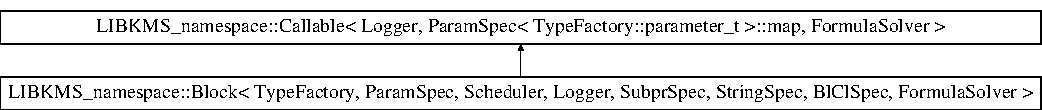
\includegraphics[height=1.483444cm]{classLIBKMS__namespace_1_1Block}
\end{center}
\end{figure}
\subsection*{Открытые типы}
\begin{DoxyCompactItemize}
\item 
typedef \hyperlink{classLIBKMS__namespace_1_1Block}{Block}$<$ \hyperlink{classLIBKMS__namespace_1_1TypeFactory}{Type\-Factory}, \\*
Param\-Spec, Scheduler, Logger, \\*
Subpr\-Spec, String\-Spec, \\*
Bl\-Cl\-Spec, Formula\-Solver $>$ \hyperlink{classLIBKMS__namespace_1_1Block_ae33d301121e149f8c7cc9a19f7046237}{block\-\_\-t}
\item 
typedef \hyperlink{classLIBKMS__namespace_1_1TypeFactory}{Type\-Factory} \hyperlink{classLIBKMS__namespace_1_1Block_a1eac0ca1a7f0b6eb9e18a2990d3aa286}{type\-\_\-factory\-\_\-t}
\item 
typedef \hyperlink{classLIBKMS__namespace_1_1TypeFactory_a103a08b747cfe5b233b12c802b4563dc}{type\-\_\-factory\-\_\-t\-::parameter\-\_\-t} \hyperlink{classLIBKMS__namespace_1_1Block_aebb850556ee5e8369c1d95caa5dc9c69}{parameter\-\_\-t}
\item 
typedef \hyperlink{classLIBKMS__namespace_1_1Parameter_a28516bcd5bad5857b2d1c676e4176f51}{parameter\-\_\-t\-::ptr\-\_\-t} \hyperlink{classLIBKMS__namespace_1_1Block_ac67e65c4f0bd77566768ec64e25382b6}{parameter\-\_\-ptr}
\item 
typedef Param\-Spec$<$ \hyperlink{classLIBKMS__namespace_1_1Block_aebb850556ee5e8369c1d95caa5dc9c69}{parameter\-\_\-t} $>$\\*
\-::map \hyperlink{classLIBKMS__namespace_1_1Block_a8d67012b101494c21dee73cd82a1e99f}{parameter\-\_\-map}
\item 
typedef \hyperlink{classLIBKMS__namespace_1_1Callable}{Callable}$<$ Logger, \\*
\hyperlink{classLIBKMS__namespace_1_1Block_a8d67012b101494c21dee73cd82a1e99f}{parameter\-\_\-map}, Formula\-Solver $>$ \hyperlink{classLIBKMS__namespace_1_1Block_a3742cf8820e4b909e4fbcc3d9c22d686}{callable\-\_\-t}
\item 
typedef \hyperlink{classLIBKMS__namespace_1_1Subprogram}{Subprogram}$<$ Logger, \\*
\hyperlink{classLIBKMS__namespace_1_1Block_a8d67012b101494c21dee73cd82a1e99f}{parameter\-\_\-map}, Formula\-Solver $>$ \hyperlink{classLIBKMS__namespace_1_1Block_a89ead8d5558038ca06b862f1988c3d1a}{subprogram\-\_\-t}
\item 
typedef Subpr\-Spec\\*
$<$ \hyperlink{classLIBKMS__namespace_1_1Block_a89ead8d5558038ca06b862f1988c3d1a}{subprogram\-\_\-t} $>$\-::ptr \hyperlink{classLIBKMS__namespace_1_1Block_aa267fa3009a53828cb55cd853ff4c1b6}{subprogram\-\_\-ptr}
\item 
typedef Subpr\-Spec\\*
$<$ \hyperlink{classLIBKMS__namespace_1_1Block_a89ead8d5558038ca06b862f1988c3d1a}{subprogram\-\_\-t} $>$\-::map \hyperlink{classLIBKMS__namespace_1_1Block_af6ad7e673cbb2f16fe125605494e67fb}{subprogram\-\_\-map}
\item 
typedef \hyperlink{classLIBKMS__namespace_1_1FunctionStorage}{Function\-Storage}\\*
$<$ \hyperlink{classLIBKMS__namespace_1_1Block_a8d67012b101494c21dee73cd82a1e99f}{parameter\-\_\-map} $>$ \hyperlink{classLIBKMS__namespace_1_1Block_a2776c98e95ec6726f062516f0a0cf496}{function\-\_\-storage\-\_\-t}
\item 
typedef Subpr\-Spec$<$ \hyperlink{classLIBKMS__namespace_1_1Block_ae33d301121e149f8c7cc9a19f7046237}{block\-\_\-t} $>$\-::ptr \hyperlink{classLIBKMS__namespace_1_1Block_a85039a495a9c40a4425de6a5291decbe}{ptr\-\_\-t}
\item 
typedef Subpr\-Spec$<$ \hyperlink{classLIBKMS__namespace_1_1Block_ae33d301121e149f8c7cc9a19f7046237}{block\-\_\-t} $>$\-::map \hyperlink{classLIBKMS__namespace_1_1Block_aedba90f9127d999f41d7d397e691e081}{map\-\_\-t}
\item 
typedef \hyperlink{classLIBKMS__namespace_1_1BlockClassFactory}{Block\-Class\-Factory}\\*
$<$ \hyperlink{classLIBKMS__namespace_1_1Block_a2776c98e95ec6726f062516f0a0cf496}{function\-\_\-storage\-\_\-t}, \\*
\hyperlink{classLIBKMS__namespace_1_1Block_a89ead8d5558038ca06b862f1988c3d1a}{subprogram\-\_\-t}, \hyperlink{classLIBKMS__namespace_1_1Block_aa267fa3009a53828cb55cd853ff4c1b6}{subprogram\-\_\-ptr}, \\*
\hyperlink{classLIBKMS__namespace_1_1Block_a85039a495a9c40a4425de6a5291decbe}{ptr\-\_\-t}, Bl\-Cl\-Spec $>$ \hyperlink{classLIBKMS__namespace_1_1Block_abbc80ab417de8b644b70879fe6e330f5}{block\-\_\-class\-\_\-factory\-\_\-t}
\item 
typedef \\*
\hyperlink{classLIBKMS__namespace_1_1BlockClassFactory_a882880cb8a33fcc808b41e283cea2dc3}{block\-\_\-class\-\_\-factory\-\_\-t\-::block\-\_\-class\-\_\-ptr} \hyperlink{classLIBKMS__namespace_1_1Block_ae813a32e603fb01d7e86ef4afcdc91ae}{block\-\_\-class\-\_\-ptr}
\item 
typedef \\*
\hyperlink{structLIBKMS__namespace_1_1Subprogram_1_1user__exception}{subprogram\-\_\-t\-::user\-\_\-exception} \hyperlink{classLIBKMS__namespace_1_1Block_abd8589c23dd87cd24c96cf2d1a7c9d71}{subp\-\_\-user\-\_\-exception}
\end{DoxyCompactItemize}
\subsection*{Открытые члены}
\begin{DoxyCompactItemize}
\item 
\hyperlink{classLIBKMS__namespace_1_1Block_ab5d70866215bcf83e1351b3b87f6faa8}{Block} (const std\-::string classname, const std\-::string name)
\begin{DoxyCompactList}\small\item\em Конструктор класса \end{DoxyCompactList}\item 
virtual \hyperlink{classLIBKMS__namespace_1_1Block_a5a14faabdb3b2d924f8686a3a4f18967}{$\sim$\-Block} ()
\item 
double \hyperlink{classLIBKMS__namespace_1_1Block_a5ab9ab41a6f1e64bb0c2d1e5c43b72db}{get\-\_\-lastcall\-\_\-time\-\_\-plan} ()
\begin{DoxyCompactList}\small\item\em Возвращает время последнего вызова по плану \end{DoxyCompactList}\item 
void \hyperlink{classLIBKMS__namespace_1_1Block_a69d14e60cbcdd128a7a8349bcd04df20}{set\-\_\-period} (double period) noexcept
\begin{DoxyCompactList}\small\item\em Установить период вызова \end{DoxyCompactList}\item 
void \hyperlink{classLIBKMS__namespace_1_1Block_aa40076dc7823a49c1d9b3a674982621d}{make\-\_\-periodical} () noexcept
\begin{DoxyCompactList}\small\item\em Сделать блок периодическим \end{DoxyCompactList}\item 
void \hyperlink{classLIBKMS__namespace_1_1Block_a12d13e5d8452da4ac44028deb0e5de83}{make\-\_\-nonperiodical} () noexcept
\begin{DoxyCompactList}\small\item\em Сделать блок вызываемым по обновлению \end{DoxyCompactList}\item 
bool \hyperlink{classLIBKMS__namespace_1_1Block_a60f4040e8c8d04493ca228bca478b3f8}{is\-\_\-periodical} () const noexcept
\item 
double \hyperlink{classLIBKMS__namespace_1_1Block_a7aebfd8f059a5e29eb9fa680b7de3adb}{get\-\_\-period} () const noexcept
\item 
void \hyperlink{classLIBKMS__namespace_1_1Block_a7b987f3386282af15cce3ca7b6a6de96}{set\-\_\-blocked\-\_\-in\-\_\-stop} (bool bl) noexcept
\begin{DoxyCompactList}\small\item\em Установить признак блокировки в СТОПе \end{DoxyCompactList}\item 
bool \hyperlink{classLIBKMS__namespace_1_1Block_a237c80b9eda1709cd50ded2320a11c94}{is\-\_\-blocked\-\_\-in\-\_\-stop} () noexcept
\begin{DoxyCompactList}\small\item\em Проверить, является ли заблокированным в СТОПе \end{DoxyCompactList}\item 
\hyperlink{classLIBKMS__namespace_1_1Block_ae813a32e603fb01d7e86ef4afcdc91ae}{block\-\_\-class\-\_\-ptr} \hyperlink{classLIBKMS__namespace_1_1Block_a045a7ef5cf8f38f1cdd9e88f833b4df8}{get\-\_\-block\-\_\-class} ()
\item 
bool \hyperlink{classLIBKMS__namespace_1_1Block_ac4c34ca843fa50683bf6f67eaa5de7c7}{add\-\_\-variable} (const std\-::string \&name, const std\-::string \&type) noexcept
\begin{DoxyCompactList}\small\item\em Добавить переменную \end{DoxyCompactList}\item 
bool \hyperlink{classLIBKMS__namespace_1_1Block_a11ceb4187857e178a1fbe21fb5bbe3bf}{add\-\_\-variable} (const std\-::string \&name, \hyperlink{classLIBKMS__namespace_1_1Block_ac67e65c4f0bd77566768ec64e25382b6}{parameter\-\_\-ptr} \&p) noexcept
\begin{DoxyCompactList}\small\item\em Добавить уже созданную переменную \end{DoxyCompactList}\item 
\hyperlink{classLIBKMS__namespace_1_1Block_ac67e65c4f0bd77566768ec64e25382b6}{parameter\-\_\-ptr} \hyperlink{classLIBKMS__namespace_1_1Block_a865fb12a0800ec98c6ccdbc114051b74}{get\-\_\-variable} (const std\-::string \&name) const noexcept
\begin{DoxyCompactList}\small\item\em Получить указатель на переменную с именем \end{DoxyCompactList}\item 
std\-::set$<$ std\-::string $>$ \hyperlink{classLIBKMS__namespace_1_1Block_a4b04254ca77c0d2f34d76d45b8e297d2}{write\-\_\-variables} (const std\-::set$<$ std\-::string $>$ \&allowed, \hyperlink{classLIBKMS__namespace_1_1Block_a8d67012b101494c21dee73cd82a1e99f}{parameter\-\_\-map} \&val)
\item 
std\-::set$<$ std\-::string $>$ \hyperlink{classLIBKMS__namespace_1_1Block_af3cf3e07e2ea977d1b125abb6a5da96a}{get\-\_\-var\-\_\-list} (bool show\-\_\-locals) const 
\item 
const std\-::set$<$ std\-::string $>$ \hyperlink{classLIBKMS__namespace_1_1Block_ab0208151cac031b7d0465e5d80e4fd7e}{set\-\_\-names} () const noexcept
\begin{DoxyCompactList}\small\item\em Возвращает список имен переменных S\-E\-T. \end{DoxyCompactList}\item 
{\footnotesize template$<$template$<$ typename T $>$ class Iterable$>$ }\\void \hyperlink{classLIBKMS__namespace_1_1Block_a7578ee18a28d988ab83c2caad09b51d6}{set\-\_\-names\-\_\-set} (Iterable$<$ std\-::string $>$ \&names) noexcept
\begin{DoxyCompactList}\small\item\em Устанавливает имена переменных S\-E\-T. \end{DoxyCompactList}\item 
const std\-::set$<$ std\-::string $>$ \hyperlink{classLIBKMS__namespace_1_1Block_a29bbb63c82a1ca44dca3a879db824592}{use\-\_\-names} () const noexcept
\begin{DoxyCompactList}\small\item\em Возвращает список имен переменных U\-S\-E. \end{DoxyCompactList}\item 
bool \hyperlink{classLIBKMS__namespace_1_1Block_a2f86d7c526553e42af091402bd86670b}{add\-\_\-child} (const std\-::string \&name, \hyperlink{classLIBKMS__namespace_1_1Block_a85039a495a9c40a4425de6a5291decbe}{ptr\-\_\-t} \&bl)
\begin{DoxyCompactList}\small\item\em Добавить дочерний блок \end{DoxyCompactList}\item 
\hyperlink{classLIBKMS__namespace_1_1Block_a85039a495a9c40a4425de6a5291decbe}{ptr\-\_\-t} \hyperlink{classLIBKMS__namespace_1_1Block_ad78d26bc20dd3a2fbb064881c9a05be2}{get\-\_\-child} (const std\-::string \&name) const 
\item 
void \hyperlink{classLIBKMS__namespace_1_1Block_a346b2b894e22b139665a4c14b4c39ca7}{call\-\_\-child\-\_\-by\-\_\-name} (const std\-::string \&name, double time)
\begin{DoxyCompactList}\small\item\em Вызвать дочерний блок по имени \end{DoxyCompactList}\item 
void \hyperlink{classLIBKMS__namespace_1_1Block_aa8c287cbddd60507635837e6f9b80f75}{call\-\_\-child} (\hyperlink{classLIBKMS__namespace_1_1Block_ae33d301121e149f8c7cc9a19f7046237}{block\-\_\-t} \&bl, double time)
\begin{DoxyCompactList}\small\item\em Вызвать дочерний блок \end{DoxyCompactList}\item 
bool \hyperlink{classLIBKMS__namespace_1_1Block_ac6de19c8495f98c83949dc70b981752f}{add\-\_\-subprog} (const std\-::string \&id, \hyperlink{classLIBKMS__namespace_1_1Block_aa267fa3009a53828cb55cd853ff4c1b6}{subprogram\-\_\-ptr} \&s)
\begin{DoxyCompactList}\small\item\em Добавить подпрограмму с приоритетом \end{DoxyCompactList}\item 
\hyperlink{classLIBKMS__namespace_1_1Block_aa267fa3009a53828cb55cd853ff4c1b6}{subprogram\-\_\-ptr} \hyperlink{classLIBKMS__namespace_1_1Block_a8687ab032807e767e74d002b546364b7}{get\-\_\-subprog} (const std\-::string \&name)
\begin{DoxyCompactList}\small\item\em Найти подпрограмму с заданным именем \end{DoxyCompactList}\item 
std\-::set$<$ std\-::string $>$ \hyperlink{classLIBKMS__namespace_1_1Block_a5145a4cbdf4f2f82e25a5dc30e625f53}{get\-\_\-subp\-\_\-list} (bool show\-\_\-locals) const 
\item 
bool \hyperlink{classLIBKMS__namespace_1_1Block_afe9599aa88516b84f5710216cd5ed85a}{add\-\_\-return\-\_\-param} (const std\-::string \&src\-\_\-name, const std\-::string \&dst\-\_\-name)
\item 
bool \hyperlink{classLIBKMS__namespace_1_1Block_a6b270518bc9d758d72e50a835cac5a9f}{add\-\_\-use\-\_\-param} (const std\-::string \&src\-\_\-name, const std\-::string \&dst\-\_\-name)
\item 
void \hyperlink{classLIBKMS__namespace_1_1Block_a65c37b5d072c50d71c416676196663ac}{set\-\_\-prev\-\_\-power} (bool power)
\begin{DoxyCompactList}\small\item\em Установить признак включения на предыдущем шаге \end{DoxyCompactList}\item 
bool \hyperlink{classLIBKMS__namespace_1_1Block_ad5cbf3d42dd4c5098c894ff5df6c7f21}{get\-\_\-prev\-\_\-power} () const 
\begin{DoxyCompactList}\small\item\em Получить признак включения на предыдущем шаге \end{DoxyCompactList}\item 
void \hyperlink{classLIBKMS__namespace_1_1Block_ade9aea609aecf6bfc8664003e5f0d33c}{set\-\_\-poweron\-\_\-vars} (const \hyperlink{classLIBKMS__namespace_1_1Block_a8d67012b101494c21dee73cd82a1e99f}{parameter\-\_\-map} \&p)
\begin{DoxyCompactList}\small\item\em Установить словарь переменных, записываемых по включению модуля \end{DoxyCompactList}\item 
void \hyperlink{classLIBKMS__namespace_1_1Block_a1976ce5bedc5c014cc7444a53009d5a9}{set\-\_\-poweroff\-\_\-vars} (const \hyperlink{classLIBKMS__namespace_1_1Block_a8d67012b101494c21dee73cd82a1e99f}{parameter\-\_\-map} \&p)
\begin{DoxyCompactList}\small\item\em Установить словарь переменных, записываемых по выключению модуля \end{DoxyCompactList}\item 
\hyperlink{classLIBKMS__namespace_1_1Block_a8d67012b101494c21dee73cd82a1e99f}{parameter\-\_\-map} \hyperlink{classLIBKMS__namespace_1_1Block_a2dbcc05db46fa70b284bb4e3fd0e6ae4}{write\-\_\-poweron\-\_\-vars} ()
\item 
\hyperlink{classLIBKMS__namespace_1_1Block_a8d67012b101494c21dee73cd82a1e99f}{parameter\-\_\-map} \hyperlink{classLIBKMS__namespace_1_1Block_a9576f7464cb1111775fa2f07c2c30937}{write\-\_\-poweroff\-\_\-vars} ()
\item 
\hyperlink{classLIBKMS__namespace_1_1Block_a8d67012b101494c21dee73cd82a1e99f}{parameter\-\_\-map} \hyperlink{classLIBKMS__namespace_1_1Block_a526864a3f11d6bbfdd2c5df34386c19d}{call} (double time, const \hyperlink{classLIBKMS__namespace_1_1Block_a8d67012b101494c21dee73cd82a1e99f}{parameter\-\_\-map} \&vars, const \hyperlink{classLIBKMS__namespace_1_1Block_a8d67012b101494c21dee73cd82a1e99f}{parameter\-\_\-map} \&upper)
\item 
std\-::set$<$ std\-::string $>$ \hyperlink{classLIBKMS__namespace_1_1Block_a0977650092787638c559ea40fff04d64}{get\-\_\-subblocks\-\_\-with\-\_\-errors} ()
\item 
std\-::pair$<$ std\-::deque\\*
$<$ std\-::string $>$, size\-\_\-t $>$ \hyperlink{classLIBKMS__namespace_1_1Block_af2ed32615fbeb3e4671d4d4b35802f45}{get\-\_\-next\-\_\-errors} (size\-\_\-t max=10)
\end{DoxyCompactItemize}
\subsection*{Защищенные данные}
\begin{DoxyCompactItemize}
\item 
std\-::string \hyperlink{classLIBKMS__namespace_1_1Block_a1d39e7d7bc913e6ed550677602e74e50}{\-\_\-classname}
\end{DoxyCompactItemize}


\subsection{Подробное описание}
\subsubsection*{template$<$typename Type\-Factory, template$<$ typename U $>$ class Param\-Spec, typename Scheduler, typename Logger, template$<$ typename U $>$ class Subpr\-Spec, typename String\-Spec, template$<$ typename U $>$ class Bl\-Cl\-Spec, typename Formula\-Solver$>$class L\-I\-B\-K\-M\-S\-\_\-namespace\-::\-Block$<$ Type\-Factory, Param\-Spec, Scheduler, Logger, Subpr\-Spec, String\-Spec, Bl\-Cl\-Spec, Formula\-Solver $>$}

Шаблонный класс \hyperlink{classLIBKMS__namespace_1_1Block}{Block}, отображающий блок процесс. 

\begin{quotation}


\end{quotation}
Блок процесс (БЛП) является основной единицей моделирования. БЛП верхнего уровня является всей моделью. БЛП верхнего уровня периодически вызывается внешней подпрограммой.

БЛП может содержать в себе БЛП низшего уровня. При каждом вызове БЛП высшего уровня последовательно вызывает БЛП низшего уровня в зависимости от их приоритета и периода вызова. За порядок вызова БЛП отвечает планировщик (Scheduler). Поскольку вызов БЛП низшего уровня происходит во время работы БЛП высшего уровня, период вызова последнего не может быть меньше чем у родительского БЛП.

Для передачи параметров между БЛП служат переменные. С помощью переменных можно обеспечить обмен только между блоками одного уровня. Каждый блок имеет набор собственных (S\-E\-T) и используемых (U\-S\-E) переменных. S\-E\-T и U\-S\-E переменные должны иметь символические имена, не содержащие точек и пробелов.

При вызове БЛП низшего уровня из БЛП высшего уровня производится копирование U\-S\-E переменных БЛП низшего уровня из переменных БЛП высшего уровня. По окночнании работы БЛП низшего уровня производится копирование S\-E\-T переменных из БЛП высшего уровня. Копируются только те переменные, которые указаны во внешней конфигурации -\/ базе данных (БД). Если переменная с именем, указанным в БД, отсутствует в блоке, она не копируется. При этом должно формироваться однократное сообщение об ошибке.

Вызов БЛП, запись обновленных значений переменных и возникающие при этом ошибки фиксируются в протоколе при помощи компонента Logger.

Данный шаблонный класс является прототипом для БЛП, входящих в состав модели. Последние должны содержать следующую дополнительную информацию\-: 
\begin{DoxyItemize}
\item 
\end{DoxyItemize}

Как БЛП совершает полезную работу, т.\-е. обрабатывает U\-S\-E переменные?

Создание БЛП\-: 
\begin{DoxyItemize}
\item Объявить класс, наследующий от \hyperlink{classLIBKMS__namespace_1_1Block}{Block}. 
\item В конструкторе  
\end{DoxyItemize}

Порядок работы с БЛП\-: 
\begin{DoxyItemize}
\item ... 
\item 
\item 
\item 
\item 
\item 
\end{DoxyItemize}

\subsection{Определения типов}
\hypertarget{classLIBKMS__namespace_1_1Block_abbc80ab417de8b644b70879fe6e330f5}{\index{L\-I\-B\-K\-M\-S\-\_\-namespace\-::\-Block@{L\-I\-B\-K\-M\-S\-\_\-namespace\-::\-Block}!block\-\_\-class\-\_\-factory\-\_\-t@{block\-\_\-class\-\_\-factory\-\_\-t}}
\index{block\-\_\-class\-\_\-factory\-\_\-t@{block\-\_\-class\-\_\-factory\-\_\-t}!LIBKMS_namespace::Block@{L\-I\-B\-K\-M\-S\-\_\-namespace\-::\-Block}}
\subsubsection[{block\-\_\-class\-\_\-factory\-\_\-t}]{\setlength{\rightskip}{0pt plus 5cm}template$<$typename Type\-Factory , template$<$ typename U $>$ class Param\-Spec, typename Scheduler , typename Logger , template$<$ typename U $>$ class Subpr\-Spec, typename String\-Spec , template$<$ typename U $>$ class Bl\-Cl\-Spec, typename Formula\-Solver $>$ typedef {\bf Block\-Class\-Factory}$<$ {\bf function\-\_\-storage\-\_\-t}, {\bf subprogram\-\_\-t}, {\bf subprogram\-\_\-ptr}, {\bf ptr\-\_\-t}, Bl\-Cl\-Spec $>$ {\bf L\-I\-B\-K\-M\-S\-\_\-namespace\-::\-Block}$<$ {\bf Type\-Factory}, Param\-Spec, Scheduler, Logger, Subpr\-Spec, String\-Spec, Bl\-Cl\-Spec, Formula\-Solver $>$\-::{\bf block\-\_\-class\-\_\-factory\-\_\-t}}}\label{classLIBKMS__namespace_1_1Block_abbc80ab417de8b644b70879fe6e330f5}
\hypertarget{classLIBKMS__namespace_1_1Block_ae813a32e603fb01d7e86ef4afcdc91ae}{\index{L\-I\-B\-K\-M\-S\-\_\-namespace\-::\-Block@{L\-I\-B\-K\-M\-S\-\_\-namespace\-::\-Block}!block\-\_\-class\-\_\-ptr@{block\-\_\-class\-\_\-ptr}}
\index{block\-\_\-class\-\_\-ptr@{block\-\_\-class\-\_\-ptr}!LIBKMS_namespace::Block@{L\-I\-B\-K\-M\-S\-\_\-namespace\-::\-Block}}
\subsubsection[{block\-\_\-class\-\_\-ptr}]{\setlength{\rightskip}{0pt plus 5cm}template$<$typename Type\-Factory , template$<$ typename U $>$ class Param\-Spec, typename Scheduler , typename Logger , template$<$ typename U $>$ class Subpr\-Spec, typename String\-Spec , template$<$ typename U $>$ class Bl\-Cl\-Spec, typename Formula\-Solver $>$ typedef {\bf block\-\_\-class\-\_\-factory\-\_\-t\-::block\-\_\-class\-\_\-ptr} {\bf L\-I\-B\-K\-M\-S\-\_\-namespace\-::\-Block}$<$ {\bf Type\-Factory}, Param\-Spec, Scheduler, Logger, Subpr\-Spec, String\-Spec, Bl\-Cl\-Spec, Formula\-Solver $>$\-::{\bf block\-\_\-class\-\_\-ptr}}}\label{classLIBKMS__namespace_1_1Block_ae813a32e603fb01d7e86ef4afcdc91ae}
\hypertarget{classLIBKMS__namespace_1_1Block_ae33d301121e149f8c7cc9a19f7046237}{\index{L\-I\-B\-K\-M\-S\-\_\-namespace\-::\-Block@{L\-I\-B\-K\-M\-S\-\_\-namespace\-::\-Block}!block\-\_\-t@{block\-\_\-t}}
\index{block\-\_\-t@{block\-\_\-t}!LIBKMS_namespace::Block@{L\-I\-B\-K\-M\-S\-\_\-namespace\-::\-Block}}
\subsubsection[{block\-\_\-t}]{\setlength{\rightskip}{0pt plus 5cm}template$<$typename Type\-Factory , template$<$ typename U $>$ class Param\-Spec, typename Scheduler , typename Logger , template$<$ typename U $>$ class Subpr\-Spec, typename String\-Spec , template$<$ typename U $>$ class Bl\-Cl\-Spec, typename Formula\-Solver $>$ typedef {\bf Block}$<$ {\bf Type\-Factory}, Param\-Spec, Scheduler, Logger, Subpr\-Spec, String\-Spec, Bl\-Cl\-Spec, Formula\-Solver $>$ {\bf L\-I\-B\-K\-M\-S\-\_\-namespace\-::\-Block}$<$ {\bf Type\-Factory}, Param\-Spec, Scheduler, Logger, Subpr\-Spec, String\-Spec, Bl\-Cl\-Spec, Formula\-Solver $>$\-::{\bf block\-\_\-t}}}\label{classLIBKMS__namespace_1_1Block_ae33d301121e149f8c7cc9a19f7046237}
\hypertarget{classLIBKMS__namespace_1_1Block_a3742cf8820e4b909e4fbcc3d9c22d686}{\index{L\-I\-B\-K\-M\-S\-\_\-namespace\-::\-Block@{L\-I\-B\-K\-M\-S\-\_\-namespace\-::\-Block}!callable\-\_\-t@{callable\-\_\-t}}
\index{callable\-\_\-t@{callable\-\_\-t}!LIBKMS_namespace::Block@{L\-I\-B\-K\-M\-S\-\_\-namespace\-::\-Block}}
\subsubsection[{callable\-\_\-t}]{\setlength{\rightskip}{0pt plus 5cm}template$<$typename Type\-Factory , template$<$ typename U $>$ class Param\-Spec, typename Scheduler , typename Logger , template$<$ typename U $>$ class Subpr\-Spec, typename String\-Spec , template$<$ typename U $>$ class Bl\-Cl\-Spec, typename Formula\-Solver $>$ typedef {\bf Callable}$<$ Logger, {\bf parameter\-\_\-map}, Formula\-Solver $>$ {\bf L\-I\-B\-K\-M\-S\-\_\-namespace\-::\-Block}$<$ {\bf Type\-Factory}, Param\-Spec, Scheduler, Logger, Subpr\-Spec, String\-Spec, Bl\-Cl\-Spec, Formula\-Solver $>$\-::{\bf callable\-\_\-t}}}\label{classLIBKMS__namespace_1_1Block_a3742cf8820e4b909e4fbcc3d9c22d686}
\hypertarget{classLIBKMS__namespace_1_1Block_a2776c98e95ec6726f062516f0a0cf496}{\index{L\-I\-B\-K\-M\-S\-\_\-namespace\-::\-Block@{L\-I\-B\-K\-M\-S\-\_\-namespace\-::\-Block}!function\-\_\-storage\-\_\-t@{function\-\_\-storage\-\_\-t}}
\index{function\-\_\-storage\-\_\-t@{function\-\_\-storage\-\_\-t}!LIBKMS_namespace::Block@{L\-I\-B\-K\-M\-S\-\_\-namespace\-::\-Block}}
\subsubsection[{function\-\_\-storage\-\_\-t}]{\setlength{\rightskip}{0pt plus 5cm}template$<$typename Type\-Factory , template$<$ typename U $>$ class Param\-Spec, typename Scheduler , typename Logger , template$<$ typename U $>$ class Subpr\-Spec, typename String\-Spec , template$<$ typename U $>$ class Bl\-Cl\-Spec, typename Formula\-Solver $>$ typedef {\bf Function\-Storage}$<$ {\bf parameter\-\_\-map} $>$ {\bf L\-I\-B\-K\-M\-S\-\_\-namespace\-::\-Block}$<$ {\bf Type\-Factory}, Param\-Spec, Scheduler, Logger, Subpr\-Spec, String\-Spec, Bl\-Cl\-Spec, Formula\-Solver $>$\-::{\bf function\-\_\-storage\-\_\-t}}}\label{classLIBKMS__namespace_1_1Block_a2776c98e95ec6726f062516f0a0cf496}
\hypertarget{classLIBKMS__namespace_1_1Block_aedba90f9127d999f41d7d397e691e081}{\index{L\-I\-B\-K\-M\-S\-\_\-namespace\-::\-Block@{L\-I\-B\-K\-M\-S\-\_\-namespace\-::\-Block}!map\-\_\-t@{map\-\_\-t}}
\index{map\-\_\-t@{map\-\_\-t}!LIBKMS_namespace::Block@{L\-I\-B\-K\-M\-S\-\_\-namespace\-::\-Block}}
\subsubsection[{map\-\_\-t}]{\setlength{\rightskip}{0pt plus 5cm}template$<$typename Type\-Factory , template$<$ typename U $>$ class Param\-Spec, typename Scheduler , typename Logger , template$<$ typename U $>$ class Subpr\-Spec, typename String\-Spec , template$<$ typename U $>$ class Bl\-Cl\-Spec, typename Formula\-Solver $>$ typedef Subpr\-Spec$<$ {\bf block\-\_\-t} $>$\-::map {\bf L\-I\-B\-K\-M\-S\-\_\-namespace\-::\-Block}$<$ {\bf Type\-Factory}, Param\-Spec, Scheduler, Logger, Subpr\-Spec, String\-Spec, Bl\-Cl\-Spec, Formula\-Solver $>$\-::{\bf map\-\_\-t}}}\label{classLIBKMS__namespace_1_1Block_aedba90f9127d999f41d7d397e691e081}
\hypertarget{classLIBKMS__namespace_1_1Block_a8d67012b101494c21dee73cd82a1e99f}{\index{L\-I\-B\-K\-M\-S\-\_\-namespace\-::\-Block@{L\-I\-B\-K\-M\-S\-\_\-namespace\-::\-Block}!parameter\-\_\-map@{parameter\-\_\-map}}
\index{parameter\-\_\-map@{parameter\-\_\-map}!LIBKMS_namespace::Block@{L\-I\-B\-K\-M\-S\-\_\-namespace\-::\-Block}}
\subsubsection[{parameter\-\_\-map}]{\setlength{\rightskip}{0pt plus 5cm}template$<$typename Type\-Factory , template$<$ typename U $>$ class Param\-Spec, typename Scheduler , typename Logger , template$<$ typename U $>$ class Subpr\-Spec, typename String\-Spec , template$<$ typename U $>$ class Bl\-Cl\-Spec, typename Formula\-Solver $>$ typedef Param\-Spec$<$ {\bf parameter\-\_\-t} $>$\-::map {\bf L\-I\-B\-K\-M\-S\-\_\-namespace\-::\-Block}$<$ {\bf Type\-Factory}, Param\-Spec, Scheduler, Logger, Subpr\-Spec, String\-Spec, Bl\-Cl\-Spec, Formula\-Solver $>$\-::{\bf parameter\-\_\-map}}}\label{classLIBKMS__namespace_1_1Block_a8d67012b101494c21dee73cd82a1e99f}
\hypertarget{classLIBKMS__namespace_1_1Block_ac67e65c4f0bd77566768ec64e25382b6}{\index{L\-I\-B\-K\-M\-S\-\_\-namespace\-::\-Block@{L\-I\-B\-K\-M\-S\-\_\-namespace\-::\-Block}!parameter\-\_\-ptr@{parameter\-\_\-ptr}}
\index{parameter\-\_\-ptr@{parameter\-\_\-ptr}!LIBKMS_namespace::Block@{L\-I\-B\-K\-M\-S\-\_\-namespace\-::\-Block}}
\subsubsection[{parameter\-\_\-ptr}]{\setlength{\rightskip}{0pt plus 5cm}template$<$typename Type\-Factory , template$<$ typename U $>$ class Param\-Spec, typename Scheduler , typename Logger , template$<$ typename U $>$ class Subpr\-Spec, typename String\-Spec , template$<$ typename U $>$ class Bl\-Cl\-Spec, typename Formula\-Solver $>$ typedef {\bf parameter\-\_\-t\-::ptr\-\_\-t} {\bf L\-I\-B\-K\-M\-S\-\_\-namespace\-::\-Block}$<$ {\bf Type\-Factory}, Param\-Spec, Scheduler, Logger, Subpr\-Spec, String\-Spec, Bl\-Cl\-Spec, Formula\-Solver $>$\-::{\bf parameter\-\_\-ptr}}}\label{classLIBKMS__namespace_1_1Block_ac67e65c4f0bd77566768ec64e25382b6}
\hypertarget{classLIBKMS__namespace_1_1Block_aebb850556ee5e8369c1d95caa5dc9c69}{\index{L\-I\-B\-K\-M\-S\-\_\-namespace\-::\-Block@{L\-I\-B\-K\-M\-S\-\_\-namespace\-::\-Block}!parameter\-\_\-t@{parameter\-\_\-t}}
\index{parameter\-\_\-t@{parameter\-\_\-t}!LIBKMS_namespace::Block@{L\-I\-B\-K\-M\-S\-\_\-namespace\-::\-Block}}
\subsubsection[{parameter\-\_\-t}]{\setlength{\rightskip}{0pt plus 5cm}template$<$typename Type\-Factory , template$<$ typename U $>$ class Param\-Spec, typename Scheduler , typename Logger , template$<$ typename U $>$ class Subpr\-Spec, typename String\-Spec , template$<$ typename U $>$ class Bl\-Cl\-Spec, typename Formula\-Solver $>$ typedef {\bf type\-\_\-factory\-\_\-t\-::parameter\-\_\-t} {\bf L\-I\-B\-K\-M\-S\-\_\-namespace\-::\-Block}$<$ {\bf Type\-Factory}, Param\-Spec, Scheduler, Logger, Subpr\-Spec, String\-Spec, Bl\-Cl\-Spec, Formula\-Solver $>$\-::{\bf parameter\-\_\-t}}}\label{classLIBKMS__namespace_1_1Block_aebb850556ee5e8369c1d95caa5dc9c69}
\hypertarget{classLIBKMS__namespace_1_1Block_a85039a495a9c40a4425de6a5291decbe}{\index{L\-I\-B\-K\-M\-S\-\_\-namespace\-::\-Block@{L\-I\-B\-K\-M\-S\-\_\-namespace\-::\-Block}!ptr\-\_\-t@{ptr\-\_\-t}}
\index{ptr\-\_\-t@{ptr\-\_\-t}!LIBKMS_namespace::Block@{L\-I\-B\-K\-M\-S\-\_\-namespace\-::\-Block}}
\subsubsection[{ptr\-\_\-t}]{\setlength{\rightskip}{0pt plus 5cm}template$<$typename Type\-Factory , template$<$ typename U $>$ class Param\-Spec, typename Scheduler , typename Logger , template$<$ typename U $>$ class Subpr\-Spec, typename String\-Spec , template$<$ typename U $>$ class Bl\-Cl\-Spec, typename Formula\-Solver $>$ typedef Subpr\-Spec$<$ {\bf block\-\_\-t} $>$\-::ptr {\bf L\-I\-B\-K\-M\-S\-\_\-namespace\-::\-Block}$<$ {\bf Type\-Factory}, Param\-Spec, Scheduler, Logger, Subpr\-Spec, String\-Spec, Bl\-Cl\-Spec, Formula\-Solver $>$\-::{\bf ptr\-\_\-t}}}\label{classLIBKMS__namespace_1_1Block_a85039a495a9c40a4425de6a5291decbe}
\hypertarget{classLIBKMS__namespace_1_1Block_abd8589c23dd87cd24c96cf2d1a7c9d71}{\index{L\-I\-B\-K\-M\-S\-\_\-namespace\-::\-Block@{L\-I\-B\-K\-M\-S\-\_\-namespace\-::\-Block}!subp\-\_\-user\-\_\-exception@{subp\-\_\-user\-\_\-exception}}
\index{subp\-\_\-user\-\_\-exception@{subp\-\_\-user\-\_\-exception}!LIBKMS_namespace::Block@{L\-I\-B\-K\-M\-S\-\_\-namespace\-::\-Block}}
\subsubsection[{subp\-\_\-user\-\_\-exception}]{\setlength{\rightskip}{0pt plus 5cm}template$<$typename Type\-Factory , template$<$ typename U $>$ class Param\-Spec, typename Scheduler , typename Logger , template$<$ typename U $>$ class Subpr\-Spec, typename String\-Spec , template$<$ typename U $>$ class Bl\-Cl\-Spec, typename Formula\-Solver $>$ typedef {\bf subprogram\-\_\-t\-::user\-\_\-exception} {\bf L\-I\-B\-K\-M\-S\-\_\-namespace\-::\-Block}$<$ {\bf Type\-Factory}, Param\-Spec, Scheduler, Logger, Subpr\-Spec, String\-Spec, Bl\-Cl\-Spec, Formula\-Solver $>$\-::{\bf subp\-\_\-user\-\_\-exception}}}\label{classLIBKMS__namespace_1_1Block_abd8589c23dd87cd24c96cf2d1a7c9d71}
\hypertarget{classLIBKMS__namespace_1_1Block_af6ad7e673cbb2f16fe125605494e67fb}{\index{L\-I\-B\-K\-M\-S\-\_\-namespace\-::\-Block@{L\-I\-B\-K\-M\-S\-\_\-namespace\-::\-Block}!subprogram\-\_\-map@{subprogram\-\_\-map}}
\index{subprogram\-\_\-map@{subprogram\-\_\-map}!LIBKMS_namespace::Block@{L\-I\-B\-K\-M\-S\-\_\-namespace\-::\-Block}}
\subsubsection[{subprogram\-\_\-map}]{\setlength{\rightskip}{0pt plus 5cm}template$<$typename Type\-Factory , template$<$ typename U $>$ class Param\-Spec, typename Scheduler , typename Logger , template$<$ typename U $>$ class Subpr\-Spec, typename String\-Spec , template$<$ typename U $>$ class Bl\-Cl\-Spec, typename Formula\-Solver $>$ typedef Subpr\-Spec$<$ {\bf subprogram\-\_\-t} $>$\-::map {\bf L\-I\-B\-K\-M\-S\-\_\-namespace\-::\-Block}$<$ {\bf Type\-Factory}, Param\-Spec, Scheduler, Logger, Subpr\-Spec, String\-Spec, Bl\-Cl\-Spec, Formula\-Solver $>$\-::{\bf subprogram\-\_\-map}}}\label{classLIBKMS__namespace_1_1Block_af6ad7e673cbb2f16fe125605494e67fb}
\hypertarget{classLIBKMS__namespace_1_1Block_aa267fa3009a53828cb55cd853ff4c1b6}{\index{L\-I\-B\-K\-M\-S\-\_\-namespace\-::\-Block@{L\-I\-B\-K\-M\-S\-\_\-namespace\-::\-Block}!subprogram\-\_\-ptr@{subprogram\-\_\-ptr}}
\index{subprogram\-\_\-ptr@{subprogram\-\_\-ptr}!LIBKMS_namespace::Block@{L\-I\-B\-K\-M\-S\-\_\-namespace\-::\-Block}}
\subsubsection[{subprogram\-\_\-ptr}]{\setlength{\rightskip}{0pt plus 5cm}template$<$typename Type\-Factory , template$<$ typename U $>$ class Param\-Spec, typename Scheduler , typename Logger , template$<$ typename U $>$ class Subpr\-Spec, typename String\-Spec , template$<$ typename U $>$ class Bl\-Cl\-Spec, typename Formula\-Solver $>$ typedef Subpr\-Spec$<$ {\bf subprogram\-\_\-t} $>$\-::ptr {\bf L\-I\-B\-K\-M\-S\-\_\-namespace\-::\-Block}$<$ {\bf Type\-Factory}, Param\-Spec, Scheduler, Logger, Subpr\-Spec, String\-Spec, Bl\-Cl\-Spec, Formula\-Solver $>$\-::{\bf subprogram\-\_\-ptr}}}\label{classLIBKMS__namespace_1_1Block_aa267fa3009a53828cb55cd853ff4c1b6}
\hypertarget{classLIBKMS__namespace_1_1Block_a89ead8d5558038ca06b862f1988c3d1a}{\index{L\-I\-B\-K\-M\-S\-\_\-namespace\-::\-Block@{L\-I\-B\-K\-M\-S\-\_\-namespace\-::\-Block}!subprogram\-\_\-t@{subprogram\-\_\-t}}
\index{subprogram\-\_\-t@{subprogram\-\_\-t}!LIBKMS_namespace::Block@{L\-I\-B\-K\-M\-S\-\_\-namespace\-::\-Block}}
\subsubsection[{subprogram\-\_\-t}]{\setlength{\rightskip}{0pt plus 5cm}template$<$typename Type\-Factory , template$<$ typename U $>$ class Param\-Spec, typename Scheduler , typename Logger , template$<$ typename U $>$ class Subpr\-Spec, typename String\-Spec , template$<$ typename U $>$ class Bl\-Cl\-Spec, typename Formula\-Solver $>$ typedef {\bf Subprogram}$<$ Logger, {\bf parameter\-\_\-map}, Formula\-Solver $>$ {\bf L\-I\-B\-K\-M\-S\-\_\-namespace\-::\-Block}$<$ {\bf Type\-Factory}, Param\-Spec, Scheduler, Logger, Subpr\-Spec, String\-Spec, Bl\-Cl\-Spec, Formula\-Solver $>$\-::{\bf subprogram\-\_\-t}}}\label{classLIBKMS__namespace_1_1Block_a89ead8d5558038ca06b862f1988c3d1a}
\hypertarget{classLIBKMS__namespace_1_1Block_a1eac0ca1a7f0b6eb9e18a2990d3aa286}{\index{L\-I\-B\-K\-M\-S\-\_\-namespace\-::\-Block@{L\-I\-B\-K\-M\-S\-\_\-namespace\-::\-Block}!type\-\_\-factory\-\_\-t@{type\-\_\-factory\-\_\-t}}
\index{type\-\_\-factory\-\_\-t@{type\-\_\-factory\-\_\-t}!LIBKMS_namespace::Block@{L\-I\-B\-K\-M\-S\-\_\-namespace\-::\-Block}}
\subsubsection[{type\-\_\-factory\-\_\-t}]{\setlength{\rightskip}{0pt plus 5cm}template$<$typename Type\-Factory , template$<$ typename U $>$ class Param\-Spec, typename Scheduler , typename Logger , template$<$ typename U $>$ class Subpr\-Spec, typename String\-Spec , template$<$ typename U $>$ class Bl\-Cl\-Spec, typename Formula\-Solver $>$ typedef {\bf Type\-Factory} {\bf L\-I\-B\-K\-M\-S\-\_\-namespace\-::\-Block}$<$ {\bf Type\-Factory}, Param\-Spec, Scheduler, Logger, Subpr\-Spec, String\-Spec, Bl\-Cl\-Spec, Formula\-Solver $>$\-::{\bf type\-\_\-factory\-\_\-t}}}\label{classLIBKMS__namespace_1_1Block_a1eac0ca1a7f0b6eb9e18a2990d3aa286}


\subsection{Конструктор(ы)}
\hypertarget{classLIBKMS__namespace_1_1Block_ab5d70866215bcf83e1351b3b87f6faa8}{\index{L\-I\-B\-K\-M\-S\-\_\-namespace\-::\-Block@{L\-I\-B\-K\-M\-S\-\_\-namespace\-::\-Block}!Block@{Block}}
\index{Block@{Block}!LIBKMS_namespace::Block@{L\-I\-B\-K\-M\-S\-\_\-namespace\-::\-Block}}
\subsubsection[{Block}]{\setlength{\rightskip}{0pt plus 5cm}template$<$typename Type\-Factory , template$<$ typename U $>$ class Param\-Spec, typename Scheduler , typename Logger , template$<$ typename U $>$ class Subpr\-Spec, typename String\-Spec , template$<$ typename U $>$ class Bl\-Cl\-Spec, typename Formula\-Solver $>$ {\bf L\-I\-B\-K\-M\-S\-\_\-namespace\-::\-Block}$<$ {\bf Type\-Factory}, Param\-Spec, Scheduler, Logger, Subpr\-Spec, String\-Spec, Bl\-Cl\-Spec, Formula\-Solver $>$\-::{\bf Block} (
\begin{DoxyParamCaption}
\item[{const std\-::string}]{classname, }
\item[{const std\-::string}]{name}
\end{DoxyParamCaption}
)\hspace{0.3cm}{\ttfamily [inline]}}}\label{classLIBKMS__namespace_1_1Block_ab5d70866215bcf83e1351b3b87f6faa8}


Конструктор класса 

\hypertarget{classLIBKMS__namespace_1_1Block_a5a14faabdb3b2d924f8686a3a4f18967}{\index{L\-I\-B\-K\-M\-S\-\_\-namespace\-::\-Block@{L\-I\-B\-K\-M\-S\-\_\-namespace\-::\-Block}!$\sim$\-Block@{$\sim$\-Block}}
\index{$\sim$\-Block@{$\sim$\-Block}!LIBKMS_namespace::Block@{L\-I\-B\-K\-M\-S\-\_\-namespace\-::\-Block}}
\subsubsection[{$\sim$\-Block}]{\setlength{\rightskip}{0pt plus 5cm}template$<$typename Type\-Factory , template$<$ typename U $>$ class Param\-Spec, typename Scheduler , typename Logger , template$<$ typename U $>$ class Subpr\-Spec, typename String\-Spec , template$<$ typename U $>$ class Bl\-Cl\-Spec, typename Formula\-Solver $>$ virtual {\bf L\-I\-B\-K\-M\-S\-\_\-namespace\-::\-Block}$<$ {\bf Type\-Factory}, Param\-Spec, Scheduler, Logger, Subpr\-Spec, String\-Spec, Bl\-Cl\-Spec, Formula\-Solver $>$\-::$\sim${\bf Block} (
\begin{DoxyParamCaption}
{}
\end{DoxyParamCaption}
)\hspace{0.3cm}{\ttfamily [inline]}, {\ttfamily [virtual]}}}\label{classLIBKMS__namespace_1_1Block_a5a14faabdb3b2d924f8686a3a4f18967}


\subsection{Методы}
\hypertarget{classLIBKMS__namespace_1_1Block_a2f86d7c526553e42af091402bd86670b}{\index{L\-I\-B\-K\-M\-S\-\_\-namespace\-::\-Block@{L\-I\-B\-K\-M\-S\-\_\-namespace\-::\-Block}!add\-\_\-child@{add\-\_\-child}}
\index{add\-\_\-child@{add\-\_\-child}!LIBKMS_namespace::Block@{L\-I\-B\-K\-M\-S\-\_\-namespace\-::\-Block}}
\subsubsection[{add\-\_\-child}]{\setlength{\rightskip}{0pt plus 5cm}template$<$typename Type\-Factory , template$<$ typename U $>$ class Param\-Spec, typename Scheduler , typename Logger , template$<$ typename U $>$ class Subpr\-Spec, typename String\-Spec , template$<$ typename U $>$ class Bl\-Cl\-Spec, typename Formula\-Solver $>$ bool {\bf L\-I\-B\-K\-M\-S\-\_\-namespace\-::\-Block}$<$ {\bf Type\-Factory}, Param\-Spec, Scheduler, Logger, Subpr\-Spec, String\-Spec, Bl\-Cl\-Spec, Formula\-Solver $>$\-::add\-\_\-child (
\begin{DoxyParamCaption}
\item[{const std\-::string \&}]{name, }
\item[{{\bf ptr\-\_\-t} \&}]{bl}
\end{DoxyParamCaption}
)\hspace{0.3cm}{\ttfamily [inline]}}}\label{classLIBKMS__namespace_1_1Block_a2f86d7c526553e42af091402bd86670b}


Добавить дочерний блок 

\hypertarget{classLIBKMS__namespace_1_1Block_afe9599aa88516b84f5710216cd5ed85a}{\index{L\-I\-B\-K\-M\-S\-\_\-namespace\-::\-Block@{L\-I\-B\-K\-M\-S\-\_\-namespace\-::\-Block}!add\-\_\-return\-\_\-param@{add\-\_\-return\-\_\-param}}
\index{add\-\_\-return\-\_\-param@{add\-\_\-return\-\_\-param}!LIBKMS_namespace::Block@{L\-I\-B\-K\-M\-S\-\_\-namespace\-::\-Block}}
\subsubsection[{add\-\_\-return\-\_\-param}]{\setlength{\rightskip}{0pt plus 5cm}template$<$typename Type\-Factory , template$<$ typename U $>$ class Param\-Spec, typename Scheduler , typename Logger , template$<$ typename U $>$ class Subpr\-Spec, typename String\-Spec , template$<$ typename U $>$ class Bl\-Cl\-Spec, typename Formula\-Solver $>$ bool {\bf L\-I\-B\-K\-M\-S\-\_\-namespace\-::\-Block}$<$ {\bf Type\-Factory}, Param\-Spec, Scheduler, Logger, Subpr\-Spec, String\-Spec, Bl\-Cl\-Spec, Formula\-Solver $>$\-::add\-\_\-return\-\_\-param (
\begin{DoxyParamCaption}
\item[{const std\-::string \&}]{src\-\_\-name, }
\item[{const std\-::string \&}]{dst\-\_\-name}
\end{DoxyParamCaption}
)\hspace{0.3cm}{\ttfamily [inline]}}}\label{classLIBKMS__namespace_1_1Block_afe9599aa88516b84f5710216cd5ed85a}
Добавить переменную, возвращаемую при вызове 
\begin{DoxyParams}{Аргументы}
{\em src\-\_\-name} & имя переменной источника, расположенной в этом блоке \\
\hline
{\em dst\-\_\-name} & имя переменной назначения, расположенной в блоке уровнем выше \\
\hline
\end{DoxyParams}
\hypertarget{classLIBKMS__namespace_1_1Block_ac6de19c8495f98c83949dc70b981752f}{\index{L\-I\-B\-K\-M\-S\-\_\-namespace\-::\-Block@{L\-I\-B\-K\-M\-S\-\_\-namespace\-::\-Block}!add\-\_\-subprog@{add\-\_\-subprog}}
\index{add\-\_\-subprog@{add\-\_\-subprog}!LIBKMS_namespace::Block@{L\-I\-B\-K\-M\-S\-\_\-namespace\-::\-Block}}
\subsubsection[{add\-\_\-subprog}]{\setlength{\rightskip}{0pt plus 5cm}template$<$typename Type\-Factory , template$<$ typename U $>$ class Param\-Spec, typename Scheduler , typename Logger , template$<$ typename U $>$ class Subpr\-Spec, typename String\-Spec , template$<$ typename U $>$ class Bl\-Cl\-Spec, typename Formula\-Solver $>$ bool {\bf L\-I\-B\-K\-M\-S\-\_\-namespace\-::\-Block}$<$ {\bf Type\-Factory}, Param\-Spec, Scheduler, Logger, Subpr\-Spec, String\-Spec, Bl\-Cl\-Spec, Formula\-Solver $>$\-::add\-\_\-subprog (
\begin{DoxyParamCaption}
\item[{const std\-::string \&}]{id, }
\item[{{\bf subprogram\-\_\-ptr} \&}]{s}
\end{DoxyParamCaption}
)\hspace{0.3cm}{\ttfamily [inline]}}}\label{classLIBKMS__namespace_1_1Block_ac6de19c8495f98c83949dc70b981752f}


Добавить подпрограмму с приоритетом 

\hypertarget{classLIBKMS__namespace_1_1Block_a6b270518bc9d758d72e50a835cac5a9f}{\index{L\-I\-B\-K\-M\-S\-\_\-namespace\-::\-Block@{L\-I\-B\-K\-M\-S\-\_\-namespace\-::\-Block}!add\-\_\-use\-\_\-param@{add\-\_\-use\-\_\-param}}
\index{add\-\_\-use\-\_\-param@{add\-\_\-use\-\_\-param}!LIBKMS_namespace::Block@{L\-I\-B\-K\-M\-S\-\_\-namespace\-::\-Block}}
\subsubsection[{add\-\_\-use\-\_\-param}]{\setlength{\rightskip}{0pt plus 5cm}template$<$typename Type\-Factory , template$<$ typename U $>$ class Param\-Spec, typename Scheduler , typename Logger , template$<$ typename U $>$ class Subpr\-Spec, typename String\-Spec , template$<$ typename U $>$ class Bl\-Cl\-Spec, typename Formula\-Solver $>$ bool {\bf L\-I\-B\-K\-M\-S\-\_\-namespace\-::\-Block}$<$ {\bf Type\-Factory}, Param\-Spec, Scheduler, Logger, Subpr\-Spec, String\-Spec, Bl\-Cl\-Spec, Formula\-Solver $>$\-::add\-\_\-use\-\_\-param (
\begin{DoxyParamCaption}
\item[{const std\-::string \&}]{src\-\_\-name, }
\item[{const std\-::string \&}]{dst\-\_\-name}
\end{DoxyParamCaption}
)\hspace{0.3cm}{\ttfamily [inline]}}}\label{classLIBKMS__namespace_1_1Block_a6b270518bc9d758d72e50a835cac5a9f}
Добавить переменную, копируемую из блока уровнем выше 
\begin{DoxyParams}{Аргументы}
{\em src\-\_\-name} & имя переменной в блоке уровнем выше \\
\hline
{\em dst\-\_\-name} & имя переменной в этом блоке \\
\hline
\end{DoxyParams}
\hypertarget{classLIBKMS__namespace_1_1Block_ac4c34ca843fa50683bf6f67eaa5de7c7}{\index{L\-I\-B\-K\-M\-S\-\_\-namespace\-::\-Block@{L\-I\-B\-K\-M\-S\-\_\-namespace\-::\-Block}!add\-\_\-variable@{add\-\_\-variable}}
\index{add\-\_\-variable@{add\-\_\-variable}!LIBKMS_namespace::Block@{L\-I\-B\-K\-M\-S\-\_\-namespace\-::\-Block}}
\subsubsection[{add\-\_\-variable}]{\setlength{\rightskip}{0pt plus 5cm}template$<$typename Type\-Factory , template$<$ typename U $>$ class Param\-Spec, typename Scheduler , typename Logger , template$<$ typename U $>$ class Subpr\-Spec, typename String\-Spec , template$<$ typename U $>$ class Bl\-Cl\-Spec, typename Formula\-Solver $>$ bool {\bf L\-I\-B\-K\-M\-S\-\_\-namespace\-::\-Block}$<$ {\bf Type\-Factory}, Param\-Spec, Scheduler, Logger, Subpr\-Spec, String\-Spec, Bl\-Cl\-Spec, Formula\-Solver $>$\-::add\-\_\-variable (
\begin{DoxyParamCaption}
\item[{const std\-::string \&}]{name, }
\item[{const std\-::string \&}]{type}
\end{DoxyParamCaption}
)\hspace{0.3cm}{\ttfamily [inline]}, {\ttfamily [noexcept]}}}\label{classLIBKMS__namespace_1_1Block_ac4c34ca843fa50683bf6f67eaa5de7c7}


Добавить переменную 

\hypertarget{classLIBKMS__namespace_1_1Block_a11ceb4187857e178a1fbe21fb5bbe3bf}{\index{L\-I\-B\-K\-M\-S\-\_\-namespace\-::\-Block@{L\-I\-B\-K\-M\-S\-\_\-namespace\-::\-Block}!add\-\_\-variable@{add\-\_\-variable}}
\index{add\-\_\-variable@{add\-\_\-variable}!LIBKMS_namespace::Block@{L\-I\-B\-K\-M\-S\-\_\-namespace\-::\-Block}}
\subsubsection[{add\-\_\-variable}]{\setlength{\rightskip}{0pt plus 5cm}template$<$typename Type\-Factory , template$<$ typename U $>$ class Param\-Spec, typename Scheduler , typename Logger , template$<$ typename U $>$ class Subpr\-Spec, typename String\-Spec , template$<$ typename U $>$ class Bl\-Cl\-Spec, typename Formula\-Solver $>$ bool {\bf L\-I\-B\-K\-M\-S\-\_\-namespace\-::\-Block}$<$ {\bf Type\-Factory}, Param\-Spec, Scheduler, Logger, Subpr\-Spec, String\-Spec, Bl\-Cl\-Spec, Formula\-Solver $>$\-::add\-\_\-variable (
\begin{DoxyParamCaption}
\item[{const std\-::string \&}]{name, }
\item[{{\bf parameter\-\_\-ptr} \&}]{p}
\end{DoxyParamCaption}
)\hspace{0.3cm}{\ttfamily [inline]}, {\ttfamily [noexcept]}}}\label{classLIBKMS__namespace_1_1Block_a11ceb4187857e178a1fbe21fb5bbe3bf}


Добавить уже созданную переменную 

\hypertarget{classLIBKMS__namespace_1_1Block_a526864a3f11d6bbfdd2c5df34386c19d}{\index{L\-I\-B\-K\-M\-S\-\_\-namespace\-::\-Block@{L\-I\-B\-K\-M\-S\-\_\-namespace\-::\-Block}!call@{call}}
\index{call@{call}!LIBKMS_namespace::Block@{L\-I\-B\-K\-M\-S\-\_\-namespace\-::\-Block}}
\subsubsection[{call}]{\setlength{\rightskip}{0pt plus 5cm}template$<$typename Type\-Factory , template$<$ typename U $>$ class Param\-Spec, typename Scheduler , typename Logger , template$<$ typename U $>$ class Subpr\-Spec, typename String\-Spec , template$<$ typename U $>$ class Bl\-Cl\-Spec, typename Formula\-Solver $>$ {\bf parameter\-\_\-map} {\bf L\-I\-B\-K\-M\-S\-\_\-namespace\-::\-Block}$<$ {\bf Type\-Factory}, Param\-Spec, Scheduler, Logger, Subpr\-Spec, String\-Spec, Bl\-Cl\-Spec, Formula\-Solver $>$\-::call (
\begin{DoxyParamCaption}
\item[{double}]{time, }
\item[{const {\bf parameter\-\_\-map} \&}]{vars, }
\item[{const {\bf parameter\-\_\-map} \&}]{upper}
\end{DoxyParamCaption}
)\hspace{0.3cm}{\ttfamily [inline]}}}\label{classLIBKMS__namespace_1_1Block_a526864a3f11d6bbfdd2c5df34386c19d}
Для вызова блока извне 
\begin{DoxyParams}{Аргументы}
{\em vars} & массив переменных для использования в блоке \\
\hline
{\em upper} & массив переменных блока более высокого уровня \\
\hline
\end{DoxyParams}
\begin{DoxyReturn}{Возвращает}
массив S\-E\-T переменных 
\end{DoxyReturn}
Задний фронт питания \hypertarget{classLIBKMS__namespace_1_1Block_aa8c287cbddd60507635837e6f9b80f75}{\index{L\-I\-B\-K\-M\-S\-\_\-namespace\-::\-Block@{L\-I\-B\-K\-M\-S\-\_\-namespace\-::\-Block}!call\-\_\-child@{call\-\_\-child}}
\index{call\-\_\-child@{call\-\_\-child}!LIBKMS_namespace::Block@{L\-I\-B\-K\-M\-S\-\_\-namespace\-::\-Block}}
\subsubsection[{call\-\_\-child}]{\setlength{\rightskip}{0pt plus 5cm}template$<$typename Type\-Factory , template$<$ typename U $>$ class Param\-Spec, typename Scheduler , typename Logger , template$<$ typename U $>$ class Subpr\-Spec, typename String\-Spec , template$<$ typename U $>$ class Bl\-Cl\-Spec, typename Formula\-Solver $>$ void {\bf L\-I\-B\-K\-M\-S\-\_\-namespace\-::\-Block}$<$ {\bf Type\-Factory}, Param\-Spec, Scheduler, Logger, Subpr\-Spec, String\-Spec, Bl\-Cl\-Spec, Formula\-Solver $>$\-::call\-\_\-child (
\begin{DoxyParamCaption}
\item[{{\bf block\-\_\-t} \&}]{bl, }
\item[{double}]{time}
\end{DoxyParamCaption}
)\hspace{0.3cm}{\ttfamily [inline]}}}\label{classLIBKMS__namespace_1_1Block_aa8c287cbddd60507635837e6f9b80f75}


Вызвать дочерний блок 

\hypertarget{classLIBKMS__namespace_1_1Block_a346b2b894e22b139665a4c14b4c39ca7}{\index{L\-I\-B\-K\-M\-S\-\_\-namespace\-::\-Block@{L\-I\-B\-K\-M\-S\-\_\-namespace\-::\-Block}!call\-\_\-child\-\_\-by\-\_\-name@{call\-\_\-child\-\_\-by\-\_\-name}}
\index{call\-\_\-child\-\_\-by\-\_\-name@{call\-\_\-child\-\_\-by\-\_\-name}!LIBKMS_namespace::Block@{L\-I\-B\-K\-M\-S\-\_\-namespace\-::\-Block}}
\subsubsection[{call\-\_\-child\-\_\-by\-\_\-name}]{\setlength{\rightskip}{0pt plus 5cm}template$<$typename Type\-Factory , template$<$ typename U $>$ class Param\-Spec, typename Scheduler , typename Logger , template$<$ typename U $>$ class Subpr\-Spec, typename String\-Spec , template$<$ typename U $>$ class Bl\-Cl\-Spec, typename Formula\-Solver $>$ void {\bf L\-I\-B\-K\-M\-S\-\_\-namespace\-::\-Block}$<$ {\bf Type\-Factory}, Param\-Spec, Scheduler, Logger, Subpr\-Spec, String\-Spec, Bl\-Cl\-Spec, Formula\-Solver $>$\-::call\-\_\-child\-\_\-by\-\_\-name (
\begin{DoxyParamCaption}
\item[{const std\-::string \&}]{name, }
\item[{double}]{time}
\end{DoxyParamCaption}
)\hspace{0.3cm}{\ttfamily [inline]}}}\label{classLIBKMS__namespace_1_1Block_a346b2b894e22b139665a4c14b4c39ca7}


Вызвать дочерний блок по имени 

\hypertarget{classLIBKMS__namespace_1_1Block_a045a7ef5cf8f38f1cdd9e88f833b4df8}{\index{L\-I\-B\-K\-M\-S\-\_\-namespace\-::\-Block@{L\-I\-B\-K\-M\-S\-\_\-namespace\-::\-Block}!get\-\_\-block\-\_\-class@{get\-\_\-block\-\_\-class}}
\index{get\-\_\-block\-\_\-class@{get\-\_\-block\-\_\-class}!LIBKMS_namespace::Block@{L\-I\-B\-K\-M\-S\-\_\-namespace\-::\-Block}}
\subsubsection[{get\-\_\-block\-\_\-class}]{\setlength{\rightskip}{0pt plus 5cm}template$<$typename Type\-Factory , template$<$ typename U $>$ class Param\-Spec, typename Scheduler , typename Logger , template$<$ typename U $>$ class Subpr\-Spec, typename String\-Spec , template$<$ typename U $>$ class Bl\-Cl\-Spec, typename Formula\-Solver $>$ {\bf block\-\_\-class\-\_\-ptr} {\bf L\-I\-B\-K\-M\-S\-\_\-namespace\-::\-Block}$<$ {\bf Type\-Factory}, Param\-Spec, Scheduler, Logger, Subpr\-Spec, String\-Spec, Bl\-Cl\-Spec, Formula\-Solver $>$\-::get\-\_\-block\-\_\-class (
\begin{DoxyParamCaption}
{}
\end{DoxyParamCaption}
)\hspace{0.3cm}{\ttfamily [inline]}}}\label{classLIBKMS__namespace_1_1Block_a045a7ef5cf8f38f1cdd9e88f833b4df8}
\hypertarget{classLIBKMS__namespace_1_1Block_ad78d26bc20dd3a2fbb064881c9a05be2}{\index{L\-I\-B\-K\-M\-S\-\_\-namespace\-::\-Block@{L\-I\-B\-K\-M\-S\-\_\-namespace\-::\-Block}!get\-\_\-child@{get\-\_\-child}}
\index{get\-\_\-child@{get\-\_\-child}!LIBKMS_namespace::Block@{L\-I\-B\-K\-M\-S\-\_\-namespace\-::\-Block}}
\subsubsection[{get\-\_\-child}]{\setlength{\rightskip}{0pt plus 5cm}template$<$typename Type\-Factory , template$<$ typename U $>$ class Param\-Spec, typename Scheduler , typename Logger , template$<$ typename U $>$ class Subpr\-Spec, typename String\-Spec , template$<$ typename U $>$ class Bl\-Cl\-Spec, typename Formula\-Solver $>$ {\bf ptr\-\_\-t} {\bf L\-I\-B\-K\-M\-S\-\_\-namespace\-::\-Block}$<$ {\bf Type\-Factory}, Param\-Spec, Scheduler, Logger, Subpr\-Spec, String\-Spec, Bl\-Cl\-Spec, Formula\-Solver $>$\-::get\-\_\-child (
\begin{DoxyParamCaption}
\item[{const std\-::string \&}]{name}
\end{DoxyParamCaption}
) const\hspace{0.3cm}{\ttfamily [inline]}}}\label{classLIBKMS__namespace_1_1Block_ad78d26bc20dd3a2fbb064881c9a05be2}
\hypertarget{classLIBKMS__namespace_1_1Block_a5ab9ab41a6f1e64bb0c2d1e5c43b72db}{\index{L\-I\-B\-K\-M\-S\-\_\-namespace\-::\-Block@{L\-I\-B\-K\-M\-S\-\_\-namespace\-::\-Block}!get\-\_\-lastcall\-\_\-time\-\_\-plan@{get\-\_\-lastcall\-\_\-time\-\_\-plan}}
\index{get\-\_\-lastcall\-\_\-time\-\_\-plan@{get\-\_\-lastcall\-\_\-time\-\_\-plan}!LIBKMS_namespace::Block@{L\-I\-B\-K\-M\-S\-\_\-namespace\-::\-Block}}
\subsubsection[{get\-\_\-lastcall\-\_\-time\-\_\-plan}]{\setlength{\rightskip}{0pt plus 5cm}template$<$typename Type\-Factory , template$<$ typename U $>$ class Param\-Spec, typename Scheduler , typename Logger , template$<$ typename U $>$ class Subpr\-Spec, typename String\-Spec , template$<$ typename U $>$ class Bl\-Cl\-Spec, typename Formula\-Solver $>$ double {\bf L\-I\-B\-K\-M\-S\-\_\-namespace\-::\-Block}$<$ {\bf Type\-Factory}, Param\-Spec, Scheduler, Logger, Subpr\-Spec, String\-Spec, Bl\-Cl\-Spec, Formula\-Solver $>$\-::get\-\_\-lastcall\-\_\-time\-\_\-plan (
\begin{DoxyParamCaption}
{}
\end{DoxyParamCaption}
)\hspace{0.3cm}{\ttfamily [inline]}}}\label{classLIBKMS__namespace_1_1Block_a5ab9ab41a6f1e64bb0c2d1e5c43b72db}


Возвращает время последнего вызова по плану 

\hypertarget{classLIBKMS__namespace_1_1Block_af2ed32615fbeb3e4671d4d4b35802f45}{\index{L\-I\-B\-K\-M\-S\-\_\-namespace\-::\-Block@{L\-I\-B\-K\-M\-S\-\_\-namespace\-::\-Block}!get\-\_\-next\-\_\-errors@{get\-\_\-next\-\_\-errors}}
\index{get\-\_\-next\-\_\-errors@{get\-\_\-next\-\_\-errors}!LIBKMS_namespace::Block@{L\-I\-B\-K\-M\-S\-\_\-namespace\-::\-Block}}
\subsubsection[{get\-\_\-next\-\_\-errors}]{\setlength{\rightskip}{0pt plus 5cm}template$<$typename Type\-Factory , template$<$ typename U $>$ class Param\-Spec, typename Scheduler , typename Logger , template$<$ typename U $>$ class Subpr\-Spec, typename String\-Spec , template$<$ typename U $>$ class Bl\-Cl\-Spec, typename Formula\-Solver $>$ std\-::pair$<$ std\-::deque$<$ std\-::string $>$, size\-\_\-t $>$ {\bf L\-I\-B\-K\-M\-S\-\_\-namespace\-::\-Block}$<$ {\bf Type\-Factory}, Param\-Spec, Scheduler, Logger, Subpr\-Spec, String\-Spec, Bl\-Cl\-Spec, Formula\-Solver $>$\-::get\-\_\-next\-\_\-errors (
\begin{DoxyParamCaption}
\item[{size\-\_\-t}]{max = {\ttfamily 10}}
\end{DoxyParamCaption}
)\hspace{0.3cm}{\ttfamily [inline]}}}\label{classLIBKMS__namespace_1_1Block_af2ed32615fbeb3e4671d4d4b35802f45}
\hypertarget{classLIBKMS__namespace_1_1Block_a7aebfd8f059a5e29eb9fa680b7de3adb}{\index{L\-I\-B\-K\-M\-S\-\_\-namespace\-::\-Block@{L\-I\-B\-K\-M\-S\-\_\-namespace\-::\-Block}!get\-\_\-period@{get\-\_\-period}}
\index{get\-\_\-period@{get\-\_\-period}!LIBKMS_namespace::Block@{L\-I\-B\-K\-M\-S\-\_\-namespace\-::\-Block}}
\subsubsection[{get\-\_\-period}]{\setlength{\rightskip}{0pt plus 5cm}template$<$typename Type\-Factory , template$<$ typename U $>$ class Param\-Spec, typename Scheduler , typename Logger , template$<$ typename U $>$ class Subpr\-Spec, typename String\-Spec , template$<$ typename U $>$ class Bl\-Cl\-Spec, typename Formula\-Solver $>$ double {\bf L\-I\-B\-K\-M\-S\-\_\-namespace\-::\-Block}$<$ {\bf Type\-Factory}, Param\-Spec, Scheduler, Logger, Subpr\-Spec, String\-Spec, Bl\-Cl\-Spec, Formula\-Solver $>$\-::get\-\_\-period (
\begin{DoxyParamCaption}
{}
\end{DoxyParamCaption}
) const\hspace{0.3cm}{\ttfamily [inline]}, {\ttfamily [noexcept]}}}\label{classLIBKMS__namespace_1_1Block_a7aebfd8f059a5e29eb9fa680b7de3adb}
\hypertarget{classLIBKMS__namespace_1_1Block_ad5cbf3d42dd4c5098c894ff5df6c7f21}{\index{L\-I\-B\-K\-M\-S\-\_\-namespace\-::\-Block@{L\-I\-B\-K\-M\-S\-\_\-namespace\-::\-Block}!get\-\_\-prev\-\_\-power@{get\-\_\-prev\-\_\-power}}
\index{get\-\_\-prev\-\_\-power@{get\-\_\-prev\-\_\-power}!LIBKMS_namespace::Block@{L\-I\-B\-K\-M\-S\-\_\-namespace\-::\-Block}}
\subsubsection[{get\-\_\-prev\-\_\-power}]{\setlength{\rightskip}{0pt plus 5cm}template$<$typename Type\-Factory , template$<$ typename U $>$ class Param\-Spec, typename Scheduler , typename Logger , template$<$ typename U $>$ class Subpr\-Spec, typename String\-Spec , template$<$ typename U $>$ class Bl\-Cl\-Spec, typename Formula\-Solver $>$ bool {\bf L\-I\-B\-K\-M\-S\-\_\-namespace\-::\-Block}$<$ {\bf Type\-Factory}, Param\-Spec, Scheduler, Logger, Subpr\-Spec, String\-Spec, Bl\-Cl\-Spec, Formula\-Solver $>$\-::get\-\_\-prev\-\_\-power (
\begin{DoxyParamCaption}
{}
\end{DoxyParamCaption}
) const\hspace{0.3cm}{\ttfamily [inline]}}}\label{classLIBKMS__namespace_1_1Block_ad5cbf3d42dd4c5098c894ff5df6c7f21}


Получить признак включения на предыдущем шаге 

\hypertarget{classLIBKMS__namespace_1_1Block_a0977650092787638c559ea40fff04d64}{\index{L\-I\-B\-K\-M\-S\-\_\-namespace\-::\-Block@{L\-I\-B\-K\-M\-S\-\_\-namespace\-::\-Block}!get\-\_\-subblocks\-\_\-with\-\_\-errors@{get\-\_\-subblocks\-\_\-with\-\_\-errors}}
\index{get\-\_\-subblocks\-\_\-with\-\_\-errors@{get\-\_\-subblocks\-\_\-with\-\_\-errors}!LIBKMS_namespace::Block@{L\-I\-B\-K\-M\-S\-\_\-namespace\-::\-Block}}
\subsubsection[{get\-\_\-subblocks\-\_\-with\-\_\-errors}]{\setlength{\rightskip}{0pt plus 5cm}template$<$typename Type\-Factory , template$<$ typename U $>$ class Param\-Spec, typename Scheduler , typename Logger , template$<$ typename U $>$ class Subpr\-Spec, typename String\-Spec , template$<$ typename U $>$ class Bl\-Cl\-Spec, typename Formula\-Solver $>$ std\-::set$<$ std\-::string $>$ {\bf L\-I\-B\-K\-M\-S\-\_\-namespace\-::\-Block}$<$ {\bf Type\-Factory}, Param\-Spec, Scheduler, Logger, Subpr\-Spec, String\-Spec, Bl\-Cl\-Spec, Formula\-Solver $>$\-::get\-\_\-subblocks\-\_\-with\-\_\-errors (
\begin{DoxyParamCaption}
{}
\end{DoxyParamCaption}
)\hspace{0.3cm}{\ttfamily [inline]}}}\label{classLIBKMS__namespace_1_1Block_a0977650092787638c559ea40fff04d64}
\hypertarget{classLIBKMS__namespace_1_1Block_a5145a4cbdf4f2f82e25a5dc30e625f53}{\index{L\-I\-B\-K\-M\-S\-\_\-namespace\-::\-Block@{L\-I\-B\-K\-M\-S\-\_\-namespace\-::\-Block}!get\-\_\-subp\-\_\-list@{get\-\_\-subp\-\_\-list}}
\index{get\-\_\-subp\-\_\-list@{get\-\_\-subp\-\_\-list}!LIBKMS_namespace::Block@{L\-I\-B\-K\-M\-S\-\_\-namespace\-::\-Block}}
\subsubsection[{get\-\_\-subp\-\_\-list}]{\setlength{\rightskip}{0pt plus 5cm}template$<$typename Type\-Factory , template$<$ typename U $>$ class Param\-Spec, typename Scheduler , typename Logger , template$<$ typename U $>$ class Subpr\-Spec, typename String\-Spec , template$<$ typename U $>$ class Bl\-Cl\-Spec, typename Formula\-Solver $>$ std\-::set$<$ std\-::string $>$ {\bf L\-I\-B\-K\-M\-S\-\_\-namespace\-::\-Block}$<$ {\bf Type\-Factory}, Param\-Spec, Scheduler, Logger, Subpr\-Spec, String\-Spec, Bl\-Cl\-Spec, Formula\-Solver $>$\-::get\-\_\-subp\-\_\-list (
\begin{DoxyParamCaption}
\item[{bool}]{show\-\_\-locals}
\end{DoxyParamCaption}
) const\hspace{0.3cm}{\ttfamily [inline]}}}\label{classLIBKMS__namespace_1_1Block_a5145a4cbdf4f2f82e25a5dc30e625f53}
Вывести все подпрограммы блока \begin{DoxyReturn}{Возвращает}
множество строк с именами всех подпрограмм блока 
\end{DoxyReturn}
\hypertarget{classLIBKMS__namespace_1_1Block_a8687ab032807e767e74d002b546364b7}{\index{L\-I\-B\-K\-M\-S\-\_\-namespace\-::\-Block@{L\-I\-B\-K\-M\-S\-\_\-namespace\-::\-Block}!get\-\_\-subprog@{get\-\_\-subprog}}
\index{get\-\_\-subprog@{get\-\_\-subprog}!LIBKMS_namespace::Block@{L\-I\-B\-K\-M\-S\-\_\-namespace\-::\-Block}}
\subsubsection[{get\-\_\-subprog}]{\setlength{\rightskip}{0pt plus 5cm}template$<$typename Type\-Factory , template$<$ typename U $>$ class Param\-Spec, typename Scheduler , typename Logger , template$<$ typename U $>$ class Subpr\-Spec, typename String\-Spec , template$<$ typename U $>$ class Bl\-Cl\-Spec, typename Formula\-Solver $>$ {\bf subprogram\-\_\-ptr} {\bf L\-I\-B\-K\-M\-S\-\_\-namespace\-::\-Block}$<$ {\bf Type\-Factory}, Param\-Spec, Scheduler, Logger, Subpr\-Spec, String\-Spec, Bl\-Cl\-Spec, Formula\-Solver $>$\-::get\-\_\-subprog (
\begin{DoxyParamCaption}
\item[{const std\-::string \&}]{name}
\end{DoxyParamCaption}
)\hspace{0.3cm}{\ttfamily [inline]}}}\label{classLIBKMS__namespace_1_1Block_a8687ab032807e767e74d002b546364b7}


Найти подпрограмму с заданным именем 

\hypertarget{classLIBKMS__namespace_1_1Block_af3cf3e07e2ea977d1b125abb6a5da96a}{\index{L\-I\-B\-K\-M\-S\-\_\-namespace\-::\-Block@{L\-I\-B\-K\-M\-S\-\_\-namespace\-::\-Block}!get\-\_\-var\-\_\-list@{get\-\_\-var\-\_\-list}}
\index{get\-\_\-var\-\_\-list@{get\-\_\-var\-\_\-list}!LIBKMS_namespace::Block@{L\-I\-B\-K\-M\-S\-\_\-namespace\-::\-Block}}
\subsubsection[{get\-\_\-var\-\_\-list}]{\setlength{\rightskip}{0pt plus 5cm}template$<$typename Type\-Factory , template$<$ typename U $>$ class Param\-Spec, typename Scheduler , typename Logger , template$<$ typename U $>$ class Subpr\-Spec, typename String\-Spec , template$<$ typename U $>$ class Bl\-Cl\-Spec, typename Formula\-Solver $>$ std\-::set$<$ std\-::string $>$ {\bf L\-I\-B\-K\-M\-S\-\_\-namespace\-::\-Block}$<$ {\bf Type\-Factory}, Param\-Spec, Scheduler, Logger, Subpr\-Spec, String\-Spec, Bl\-Cl\-Spec, Formula\-Solver $>$\-::get\-\_\-var\-\_\-list (
\begin{DoxyParamCaption}
\item[{bool}]{show\-\_\-locals}
\end{DoxyParamCaption}
) const\hspace{0.3cm}{\ttfamily [inline]}}}\label{classLIBKMS__namespace_1_1Block_af3cf3e07e2ea977d1b125abb6a5da96a}
Вывести все переменные блока \begin{DoxyReturn}{Возвращает}
строка с описанием всех переменных блока 
\end{DoxyReturn}
\hypertarget{classLIBKMS__namespace_1_1Block_a865fb12a0800ec98c6ccdbc114051b74}{\index{L\-I\-B\-K\-M\-S\-\_\-namespace\-::\-Block@{L\-I\-B\-K\-M\-S\-\_\-namespace\-::\-Block}!get\-\_\-variable@{get\-\_\-variable}}
\index{get\-\_\-variable@{get\-\_\-variable}!LIBKMS_namespace::Block@{L\-I\-B\-K\-M\-S\-\_\-namespace\-::\-Block}}
\subsubsection[{get\-\_\-variable}]{\setlength{\rightskip}{0pt plus 5cm}template$<$typename Type\-Factory , template$<$ typename U $>$ class Param\-Spec, typename Scheduler , typename Logger , template$<$ typename U $>$ class Subpr\-Spec, typename String\-Spec , template$<$ typename U $>$ class Bl\-Cl\-Spec, typename Formula\-Solver $>$ {\bf parameter\-\_\-ptr} {\bf L\-I\-B\-K\-M\-S\-\_\-namespace\-::\-Block}$<$ {\bf Type\-Factory}, Param\-Spec, Scheduler, Logger, Subpr\-Spec, String\-Spec, Bl\-Cl\-Spec, Formula\-Solver $>$\-::get\-\_\-variable (
\begin{DoxyParamCaption}
\item[{const std\-::string \&}]{name}
\end{DoxyParamCaption}
) const\hspace{0.3cm}{\ttfamily [inline]}, {\ttfamily [noexcept]}}}\label{classLIBKMS__namespace_1_1Block_a865fb12a0800ec98c6ccdbc114051b74}


Получить указатель на переменную с именем 

\hypertarget{classLIBKMS__namespace_1_1Block_a237c80b9eda1709cd50ded2320a11c94}{\index{L\-I\-B\-K\-M\-S\-\_\-namespace\-::\-Block@{L\-I\-B\-K\-M\-S\-\_\-namespace\-::\-Block}!is\-\_\-blocked\-\_\-in\-\_\-stop@{is\-\_\-blocked\-\_\-in\-\_\-stop}}
\index{is\-\_\-blocked\-\_\-in\-\_\-stop@{is\-\_\-blocked\-\_\-in\-\_\-stop}!LIBKMS_namespace::Block@{L\-I\-B\-K\-M\-S\-\_\-namespace\-::\-Block}}
\subsubsection[{is\-\_\-blocked\-\_\-in\-\_\-stop}]{\setlength{\rightskip}{0pt plus 5cm}template$<$typename Type\-Factory , template$<$ typename U $>$ class Param\-Spec, typename Scheduler , typename Logger , template$<$ typename U $>$ class Subpr\-Spec, typename String\-Spec , template$<$ typename U $>$ class Bl\-Cl\-Spec, typename Formula\-Solver $>$ bool {\bf L\-I\-B\-K\-M\-S\-\_\-namespace\-::\-Block}$<$ {\bf Type\-Factory}, Param\-Spec, Scheduler, Logger, Subpr\-Spec, String\-Spec, Bl\-Cl\-Spec, Formula\-Solver $>$\-::is\-\_\-blocked\-\_\-in\-\_\-stop (
\begin{DoxyParamCaption}
{}
\end{DoxyParamCaption}
)\hspace{0.3cm}{\ttfamily [inline]}, {\ttfamily [noexcept]}}}\label{classLIBKMS__namespace_1_1Block_a237c80b9eda1709cd50ded2320a11c94}


Проверить, является ли заблокированным в СТОПе 

\hypertarget{classLIBKMS__namespace_1_1Block_a60f4040e8c8d04493ca228bca478b3f8}{\index{L\-I\-B\-K\-M\-S\-\_\-namespace\-::\-Block@{L\-I\-B\-K\-M\-S\-\_\-namespace\-::\-Block}!is\-\_\-periodical@{is\-\_\-periodical}}
\index{is\-\_\-periodical@{is\-\_\-periodical}!LIBKMS_namespace::Block@{L\-I\-B\-K\-M\-S\-\_\-namespace\-::\-Block}}
\subsubsection[{is\-\_\-periodical}]{\setlength{\rightskip}{0pt plus 5cm}template$<$typename Type\-Factory , template$<$ typename U $>$ class Param\-Spec, typename Scheduler , typename Logger , template$<$ typename U $>$ class Subpr\-Spec, typename String\-Spec , template$<$ typename U $>$ class Bl\-Cl\-Spec, typename Formula\-Solver $>$ bool {\bf L\-I\-B\-K\-M\-S\-\_\-namespace\-::\-Block}$<$ {\bf Type\-Factory}, Param\-Spec, Scheduler, Logger, Subpr\-Spec, String\-Spec, Bl\-Cl\-Spec, Formula\-Solver $>$\-::is\-\_\-periodical (
\begin{DoxyParamCaption}
{}
\end{DoxyParamCaption}
) const\hspace{0.3cm}{\ttfamily [inline]}, {\ttfamily [noexcept]}}}\label{classLIBKMS__namespace_1_1Block_a60f4040e8c8d04493ca228bca478b3f8}
\hypertarget{classLIBKMS__namespace_1_1Block_a12d13e5d8452da4ac44028deb0e5de83}{\index{L\-I\-B\-K\-M\-S\-\_\-namespace\-::\-Block@{L\-I\-B\-K\-M\-S\-\_\-namespace\-::\-Block}!make\-\_\-nonperiodical@{make\-\_\-nonperiodical}}
\index{make\-\_\-nonperiodical@{make\-\_\-nonperiodical}!LIBKMS_namespace::Block@{L\-I\-B\-K\-M\-S\-\_\-namespace\-::\-Block}}
\subsubsection[{make\-\_\-nonperiodical}]{\setlength{\rightskip}{0pt plus 5cm}template$<$typename Type\-Factory , template$<$ typename U $>$ class Param\-Spec, typename Scheduler , typename Logger , template$<$ typename U $>$ class Subpr\-Spec, typename String\-Spec , template$<$ typename U $>$ class Bl\-Cl\-Spec, typename Formula\-Solver $>$ void {\bf L\-I\-B\-K\-M\-S\-\_\-namespace\-::\-Block}$<$ {\bf Type\-Factory}, Param\-Spec, Scheduler, Logger, Subpr\-Spec, String\-Spec, Bl\-Cl\-Spec, Formula\-Solver $>$\-::make\-\_\-nonperiodical (
\begin{DoxyParamCaption}
{}
\end{DoxyParamCaption}
)\hspace{0.3cm}{\ttfamily [inline]}, {\ttfamily [noexcept]}}}\label{classLIBKMS__namespace_1_1Block_a12d13e5d8452da4ac44028deb0e5de83}


Сделать блок вызываемым по обновлению 

\hypertarget{classLIBKMS__namespace_1_1Block_aa40076dc7823a49c1d9b3a674982621d}{\index{L\-I\-B\-K\-M\-S\-\_\-namespace\-::\-Block@{L\-I\-B\-K\-M\-S\-\_\-namespace\-::\-Block}!make\-\_\-periodical@{make\-\_\-periodical}}
\index{make\-\_\-periodical@{make\-\_\-periodical}!LIBKMS_namespace::Block@{L\-I\-B\-K\-M\-S\-\_\-namespace\-::\-Block}}
\subsubsection[{make\-\_\-periodical}]{\setlength{\rightskip}{0pt plus 5cm}template$<$typename Type\-Factory , template$<$ typename U $>$ class Param\-Spec, typename Scheduler , typename Logger , template$<$ typename U $>$ class Subpr\-Spec, typename String\-Spec , template$<$ typename U $>$ class Bl\-Cl\-Spec, typename Formula\-Solver $>$ void {\bf L\-I\-B\-K\-M\-S\-\_\-namespace\-::\-Block}$<$ {\bf Type\-Factory}, Param\-Spec, Scheduler, Logger, Subpr\-Spec, String\-Spec, Bl\-Cl\-Spec, Formula\-Solver $>$\-::make\-\_\-periodical (
\begin{DoxyParamCaption}
{}
\end{DoxyParamCaption}
)\hspace{0.3cm}{\ttfamily [inline]}, {\ttfamily [noexcept]}}}\label{classLIBKMS__namespace_1_1Block_aa40076dc7823a49c1d9b3a674982621d}


Сделать блок периодическим 

\hypertarget{classLIBKMS__namespace_1_1Block_a7b987f3386282af15cce3ca7b6a6de96}{\index{L\-I\-B\-K\-M\-S\-\_\-namespace\-::\-Block@{L\-I\-B\-K\-M\-S\-\_\-namespace\-::\-Block}!set\-\_\-blocked\-\_\-in\-\_\-stop@{set\-\_\-blocked\-\_\-in\-\_\-stop}}
\index{set\-\_\-blocked\-\_\-in\-\_\-stop@{set\-\_\-blocked\-\_\-in\-\_\-stop}!LIBKMS_namespace::Block@{L\-I\-B\-K\-M\-S\-\_\-namespace\-::\-Block}}
\subsubsection[{set\-\_\-blocked\-\_\-in\-\_\-stop}]{\setlength{\rightskip}{0pt plus 5cm}template$<$typename Type\-Factory , template$<$ typename U $>$ class Param\-Spec, typename Scheduler , typename Logger , template$<$ typename U $>$ class Subpr\-Spec, typename String\-Spec , template$<$ typename U $>$ class Bl\-Cl\-Spec, typename Formula\-Solver $>$ void {\bf L\-I\-B\-K\-M\-S\-\_\-namespace\-::\-Block}$<$ {\bf Type\-Factory}, Param\-Spec, Scheduler, Logger, Subpr\-Spec, String\-Spec, Bl\-Cl\-Spec, Formula\-Solver $>$\-::set\-\_\-blocked\-\_\-in\-\_\-stop (
\begin{DoxyParamCaption}
\item[{bool}]{bl}
\end{DoxyParamCaption}
)\hspace{0.3cm}{\ttfamily [inline]}, {\ttfamily [noexcept]}}}\label{classLIBKMS__namespace_1_1Block_a7b987f3386282af15cce3ca7b6a6de96}


Установить признак блокировки в СТОПе 

\hypertarget{classLIBKMS__namespace_1_1Block_ab0208151cac031b7d0465e5d80e4fd7e}{\index{L\-I\-B\-K\-M\-S\-\_\-namespace\-::\-Block@{L\-I\-B\-K\-M\-S\-\_\-namespace\-::\-Block}!set\-\_\-names@{set\-\_\-names}}
\index{set\-\_\-names@{set\-\_\-names}!LIBKMS_namespace::Block@{L\-I\-B\-K\-M\-S\-\_\-namespace\-::\-Block}}
\subsubsection[{set\-\_\-names}]{\setlength{\rightskip}{0pt plus 5cm}template$<$typename Type\-Factory , template$<$ typename U $>$ class Param\-Spec, typename Scheduler , typename Logger , template$<$ typename U $>$ class Subpr\-Spec, typename String\-Spec , template$<$ typename U $>$ class Bl\-Cl\-Spec, typename Formula\-Solver $>$ const std\-::set$<$ std\-::string $>$ {\bf L\-I\-B\-K\-M\-S\-\_\-namespace\-::\-Block}$<$ {\bf Type\-Factory}, Param\-Spec, Scheduler, Logger, Subpr\-Spec, String\-Spec, Bl\-Cl\-Spec, Formula\-Solver $>$\-::set\-\_\-names (
\begin{DoxyParamCaption}
{}
\end{DoxyParamCaption}
) const\hspace{0.3cm}{\ttfamily [inline]}, {\ttfamily [noexcept]}}}\label{classLIBKMS__namespace_1_1Block_ab0208151cac031b7d0465e5d80e4fd7e}


Возвращает список имен переменных S\-E\-T. 

\hypertarget{classLIBKMS__namespace_1_1Block_a7578ee18a28d988ab83c2caad09b51d6}{\index{L\-I\-B\-K\-M\-S\-\_\-namespace\-::\-Block@{L\-I\-B\-K\-M\-S\-\_\-namespace\-::\-Block}!set\-\_\-names\-\_\-set@{set\-\_\-names\-\_\-set}}
\index{set\-\_\-names\-\_\-set@{set\-\_\-names\-\_\-set}!LIBKMS_namespace::Block@{L\-I\-B\-K\-M\-S\-\_\-namespace\-::\-Block}}
\subsubsection[{set\-\_\-names\-\_\-set}]{\setlength{\rightskip}{0pt plus 5cm}template$<$typename Type\-Factory , template$<$ typename U $>$ class Param\-Spec, typename Scheduler , typename Logger , template$<$ typename U $>$ class Subpr\-Spec, typename String\-Spec , template$<$ typename U $>$ class Bl\-Cl\-Spec, typename Formula\-Solver $>$ template$<$template$<$ typename T $>$ class Iterable$>$ void {\bf L\-I\-B\-K\-M\-S\-\_\-namespace\-::\-Block}$<$ {\bf Type\-Factory}, Param\-Spec, Scheduler, Logger, Subpr\-Spec, String\-Spec, Bl\-Cl\-Spec, Formula\-Solver $>$\-::set\-\_\-names\-\_\-set (
\begin{DoxyParamCaption}
\item[{Iterable$<$ std\-::string $>$ \&}]{names}
\end{DoxyParamCaption}
)\hspace{0.3cm}{\ttfamily [inline]}, {\ttfamily [noexcept]}}}\label{classLIBKMS__namespace_1_1Block_a7578ee18a28d988ab83c2caad09b51d6}


Устанавливает имена переменных S\-E\-T. 

\hypertarget{classLIBKMS__namespace_1_1Block_a69d14e60cbcdd128a7a8349bcd04df20}{\index{L\-I\-B\-K\-M\-S\-\_\-namespace\-::\-Block@{L\-I\-B\-K\-M\-S\-\_\-namespace\-::\-Block}!set\-\_\-period@{set\-\_\-period}}
\index{set\-\_\-period@{set\-\_\-period}!LIBKMS_namespace::Block@{L\-I\-B\-K\-M\-S\-\_\-namespace\-::\-Block}}
\subsubsection[{set\-\_\-period}]{\setlength{\rightskip}{0pt plus 5cm}template$<$typename Type\-Factory , template$<$ typename U $>$ class Param\-Spec, typename Scheduler , typename Logger , template$<$ typename U $>$ class Subpr\-Spec, typename String\-Spec , template$<$ typename U $>$ class Bl\-Cl\-Spec, typename Formula\-Solver $>$ void {\bf L\-I\-B\-K\-M\-S\-\_\-namespace\-::\-Block}$<$ {\bf Type\-Factory}, Param\-Spec, Scheduler, Logger, Subpr\-Spec, String\-Spec, Bl\-Cl\-Spec, Formula\-Solver $>$\-::set\-\_\-period (
\begin{DoxyParamCaption}
\item[{double}]{period}
\end{DoxyParamCaption}
)\hspace{0.3cm}{\ttfamily [inline]}, {\ttfamily [noexcept]}}}\label{classLIBKMS__namespace_1_1Block_a69d14e60cbcdd128a7a8349bcd04df20}


Установить период вызова 

\hypertarget{classLIBKMS__namespace_1_1Block_a1976ce5bedc5c014cc7444a53009d5a9}{\index{L\-I\-B\-K\-M\-S\-\_\-namespace\-::\-Block@{L\-I\-B\-K\-M\-S\-\_\-namespace\-::\-Block}!set\-\_\-poweroff\-\_\-vars@{set\-\_\-poweroff\-\_\-vars}}
\index{set\-\_\-poweroff\-\_\-vars@{set\-\_\-poweroff\-\_\-vars}!LIBKMS_namespace::Block@{L\-I\-B\-K\-M\-S\-\_\-namespace\-::\-Block}}
\subsubsection[{set\-\_\-poweroff\-\_\-vars}]{\setlength{\rightskip}{0pt plus 5cm}template$<$typename Type\-Factory , template$<$ typename U $>$ class Param\-Spec, typename Scheduler , typename Logger , template$<$ typename U $>$ class Subpr\-Spec, typename String\-Spec , template$<$ typename U $>$ class Bl\-Cl\-Spec, typename Formula\-Solver $>$ void {\bf L\-I\-B\-K\-M\-S\-\_\-namespace\-::\-Block}$<$ {\bf Type\-Factory}, Param\-Spec, Scheduler, Logger, Subpr\-Spec, String\-Spec, Bl\-Cl\-Spec, Formula\-Solver $>$\-::set\-\_\-poweroff\-\_\-vars (
\begin{DoxyParamCaption}
\item[{const {\bf parameter\-\_\-map} \&}]{p}
\end{DoxyParamCaption}
)\hspace{0.3cm}{\ttfamily [inline]}}}\label{classLIBKMS__namespace_1_1Block_a1976ce5bedc5c014cc7444a53009d5a9}


Установить словарь переменных, записываемых по выключению модуля 

\hypertarget{classLIBKMS__namespace_1_1Block_ade9aea609aecf6bfc8664003e5f0d33c}{\index{L\-I\-B\-K\-M\-S\-\_\-namespace\-::\-Block@{L\-I\-B\-K\-M\-S\-\_\-namespace\-::\-Block}!set\-\_\-poweron\-\_\-vars@{set\-\_\-poweron\-\_\-vars}}
\index{set\-\_\-poweron\-\_\-vars@{set\-\_\-poweron\-\_\-vars}!LIBKMS_namespace::Block@{L\-I\-B\-K\-M\-S\-\_\-namespace\-::\-Block}}
\subsubsection[{set\-\_\-poweron\-\_\-vars}]{\setlength{\rightskip}{0pt plus 5cm}template$<$typename Type\-Factory , template$<$ typename U $>$ class Param\-Spec, typename Scheduler , typename Logger , template$<$ typename U $>$ class Subpr\-Spec, typename String\-Spec , template$<$ typename U $>$ class Bl\-Cl\-Spec, typename Formula\-Solver $>$ void {\bf L\-I\-B\-K\-M\-S\-\_\-namespace\-::\-Block}$<$ {\bf Type\-Factory}, Param\-Spec, Scheduler, Logger, Subpr\-Spec, String\-Spec, Bl\-Cl\-Spec, Formula\-Solver $>$\-::set\-\_\-poweron\-\_\-vars (
\begin{DoxyParamCaption}
\item[{const {\bf parameter\-\_\-map} \&}]{p}
\end{DoxyParamCaption}
)\hspace{0.3cm}{\ttfamily [inline]}}}\label{classLIBKMS__namespace_1_1Block_ade9aea609aecf6bfc8664003e5f0d33c}


Установить словарь переменных, записываемых по включению модуля 

\hypertarget{classLIBKMS__namespace_1_1Block_a65c37b5d072c50d71c416676196663ac}{\index{L\-I\-B\-K\-M\-S\-\_\-namespace\-::\-Block@{L\-I\-B\-K\-M\-S\-\_\-namespace\-::\-Block}!set\-\_\-prev\-\_\-power@{set\-\_\-prev\-\_\-power}}
\index{set\-\_\-prev\-\_\-power@{set\-\_\-prev\-\_\-power}!LIBKMS_namespace::Block@{L\-I\-B\-K\-M\-S\-\_\-namespace\-::\-Block}}
\subsubsection[{set\-\_\-prev\-\_\-power}]{\setlength{\rightskip}{0pt plus 5cm}template$<$typename Type\-Factory , template$<$ typename U $>$ class Param\-Spec, typename Scheduler , typename Logger , template$<$ typename U $>$ class Subpr\-Spec, typename String\-Spec , template$<$ typename U $>$ class Bl\-Cl\-Spec, typename Formula\-Solver $>$ void {\bf L\-I\-B\-K\-M\-S\-\_\-namespace\-::\-Block}$<$ {\bf Type\-Factory}, Param\-Spec, Scheduler, Logger, Subpr\-Spec, String\-Spec, Bl\-Cl\-Spec, Formula\-Solver $>$\-::set\-\_\-prev\-\_\-power (
\begin{DoxyParamCaption}
\item[{bool}]{power}
\end{DoxyParamCaption}
)\hspace{0.3cm}{\ttfamily [inline]}}}\label{classLIBKMS__namespace_1_1Block_a65c37b5d072c50d71c416676196663ac}


Установить признак включения на предыдущем шаге 

\hypertarget{classLIBKMS__namespace_1_1Block_a29bbb63c82a1ca44dca3a879db824592}{\index{L\-I\-B\-K\-M\-S\-\_\-namespace\-::\-Block@{L\-I\-B\-K\-M\-S\-\_\-namespace\-::\-Block}!use\-\_\-names@{use\-\_\-names}}
\index{use\-\_\-names@{use\-\_\-names}!LIBKMS_namespace::Block@{L\-I\-B\-K\-M\-S\-\_\-namespace\-::\-Block}}
\subsubsection[{use\-\_\-names}]{\setlength{\rightskip}{0pt plus 5cm}template$<$typename Type\-Factory , template$<$ typename U $>$ class Param\-Spec, typename Scheduler , typename Logger , template$<$ typename U $>$ class Subpr\-Spec, typename String\-Spec , template$<$ typename U $>$ class Bl\-Cl\-Spec, typename Formula\-Solver $>$ const std\-::set$<$ std\-::string $>$ {\bf L\-I\-B\-K\-M\-S\-\_\-namespace\-::\-Block}$<$ {\bf Type\-Factory}, Param\-Spec, Scheduler, Logger, Subpr\-Spec, String\-Spec, Bl\-Cl\-Spec, Formula\-Solver $>$\-::use\-\_\-names (
\begin{DoxyParamCaption}
{}
\end{DoxyParamCaption}
) const\hspace{0.3cm}{\ttfamily [inline]}, {\ttfamily [noexcept]}}}\label{classLIBKMS__namespace_1_1Block_a29bbb63c82a1ca44dca3a879db824592}


Возвращает список имен переменных U\-S\-E. 

\hypertarget{classLIBKMS__namespace_1_1Block_a9576f7464cb1111775fa2f07c2c30937}{\index{L\-I\-B\-K\-M\-S\-\_\-namespace\-::\-Block@{L\-I\-B\-K\-M\-S\-\_\-namespace\-::\-Block}!write\-\_\-poweroff\-\_\-vars@{write\-\_\-poweroff\-\_\-vars}}
\index{write\-\_\-poweroff\-\_\-vars@{write\-\_\-poweroff\-\_\-vars}!LIBKMS_namespace::Block@{L\-I\-B\-K\-M\-S\-\_\-namespace\-::\-Block}}
\subsubsection[{write\-\_\-poweroff\-\_\-vars}]{\setlength{\rightskip}{0pt plus 5cm}template$<$typename Type\-Factory , template$<$ typename U $>$ class Param\-Spec, typename Scheduler , typename Logger , template$<$ typename U $>$ class Subpr\-Spec, typename String\-Spec , template$<$ typename U $>$ class Bl\-Cl\-Spec, typename Formula\-Solver $>$ {\bf parameter\-\_\-map} {\bf L\-I\-B\-K\-M\-S\-\_\-namespace\-::\-Block}$<$ {\bf Type\-Factory}, Param\-Spec, Scheduler, Logger, Subpr\-Spec, String\-Spec, Bl\-Cl\-Spec, Formula\-Solver $>$\-::write\-\_\-poweroff\-\_\-vars (
\begin{DoxyParamCaption}
{}
\end{DoxyParamCaption}
)\hspace{0.3cm}{\ttfamily [inline]}}}\label{classLIBKMS__namespace_1_1Block_a9576f7464cb1111775fa2f07c2c30937}
Записать переменные при выключении модуля \begin{DoxyReturn}{Возвращает}
Обновленные возвращаемые переменные 
\end{DoxyReturn}
\hypertarget{classLIBKMS__namespace_1_1Block_a2dbcc05db46fa70b284bb4e3fd0e6ae4}{\index{L\-I\-B\-K\-M\-S\-\_\-namespace\-::\-Block@{L\-I\-B\-K\-M\-S\-\_\-namespace\-::\-Block}!write\-\_\-poweron\-\_\-vars@{write\-\_\-poweron\-\_\-vars}}
\index{write\-\_\-poweron\-\_\-vars@{write\-\_\-poweron\-\_\-vars}!LIBKMS_namespace::Block@{L\-I\-B\-K\-M\-S\-\_\-namespace\-::\-Block}}
\subsubsection[{write\-\_\-poweron\-\_\-vars}]{\setlength{\rightskip}{0pt plus 5cm}template$<$typename Type\-Factory , template$<$ typename U $>$ class Param\-Spec, typename Scheduler , typename Logger , template$<$ typename U $>$ class Subpr\-Spec, typename String\-Spec , template$<$ typename U $>$ class Bl\-Cl\-Spec, typename Formula\-Solver $>$ {\bf parameter\-\_\-map} {\bf L\-I\-B\-K\-M\-S\-\_\-namespace\-::\-Block}$<$ {\bf Type\-Factory}, Param\-Spec, Scheduler, Logger, Subpr\-Spec, String\-Spec, Bl\-Cl\-Spec, Formula\-Solver $>$\-::write\-\_\-poweron\-\_\-vars (
\begin{DoxyParamCaption}
{}
\end{DoxyParamCaption}
)\hspace{0.3cm}{\ttfamily [inline]}}}\label{classLIBKMS__namespace_1_1Block_a2dbcc05db46fa70b284bb4e3fd0e6ae4}
Записать переменные при включении модуля \begin{DoxyReturn}{Возвращает}
Обновленные возвращаемые переменные 
\end{DoxyReturn}
\hypertarget{classLIBKMS__namespace_1_1Block_a4b04254ca77c0d2f34d76d45b8e297d2}{\index{L\-I\-B\-K\-M\-S\-\_\-namespace\-::\-Block@{L\-I\-B\-K\-M\-S\-\_\-namespace\-::\-Block}!write\-\_\-variables@{write\-\_\-variables}}
\index{write\-\_\-variables@{write\-\_\-variables}!LIBKMS_namespace::Block@{L\-I\-B\-K\-M\-S\-\_\-namespace\-::\-Block}}
\subsubsection[{write\-\_\-variables}]{\setlength{\rightskip}{0pt plus 5cm}template$<$typename Type\-Factory , template$<$ typename U $>$ class Param\-Spec, typename Scheduler , typename Logger , template$<$ typename U $>$ class Subpr\-Spec, typename String\-Spec , template$<$ typename U $>$ class Bl\-Cl\-Spec, typename Formula\-Solver $>$ std\-::set$<$ std\-::string $>$ {\bf L\-I\-B\-K\-M\-S\-\_\-namespace\-::\-Block}$<$ {\bf Type\-Factory}, Param\-Spec, Scheduler, Logger, Subpr\-Spec, String\-Spec, Bl\-Cl\-Spec, Formula\-Solver $>$\-::write\-\_\-variables (
\begin{DoxyParamCaption}
\item[{const std\-::set$<$ std\-::string $>$ \&}]{allowed, }
\item[{{\bf parameter\-\_\-map} \&}]{val}
\end{DoxyParamCaption}
)\hspace{0.3cm}{\ttfamily [inline]}}}\label{classLIBKMS__namespace_1_1Block_a4b04254ca77c0d2f34d76d45b8e297d2}
Записать значения разрешенных для записи переменных \begin{DoxyReturn}{Возвращает}
список записанных переменных 
\end{DoxyReturn}


\subsection{Данные класса}
\hypertarget{classLIBKMS__namespace_1_1Block_a1d39e7d7bc913e6ed550677602e74e50}{\index{L\-I\-B\-K\-M\-S\-\_\-namespace\-::\-Block@{L\-I\-B\-K\-M\-S\-\_\-namespace\-::\-Block}!\-\_\-classname@{\-\_\-classname}}
\index{\-\_\-classname@{\-\_\-classname}!LIBKMS_namespace::Block@{L\-I\-B\-K\-M\-S\-\_\-namespace\-::\-Block}}
\subsubsection[{\-\_\-classname}]{\setlength{\rightskip}{0pt plus 5cm}template$<$typename Type\-Factory , template$<$ typename U $>$ class Param\-Spec, typename Scheduler , typename Logger , template$<$ typename U $>$ class Subpr\-Spec, typename String\-Spec , template$<$ typename U $>$ class Bl\-Cl\-Spec, typename Formula\-Solver $>$ std\-::string {\bf L\-I\-B\-K\-M\-S\-\_\-namespace\-::\-Block}$<$ {\bf Type\-Factory}, Param\-Spec, Scheduler, Logger, Subpr\-Spec, String\-Spec, Bl\-Cl\-Spec, Formula\-Solver $>$\-::\-\_\-classname\hspace{0.3cm}{\ttfamily [protected]}}}\label{classLIBKMS__namespace_1_1Block_a1d39e7d7bc913e6ed550677602e74e50}


Объявления и описания членов класса находятся в файле\-:\begin{DoxyCompactItemize}
\item 
\hyperlink{block_8hpp}{block.\-hpp}\end{DoxyCompactItemize}

\hypertarget{structLIBKMS__namespace_1_1BlockClassFactory_1_1block__class__with__config}{\section{Шаблон структуры L\-I\-B\-K\-M\-S\-\_\-namespace\-:\-:Block\-Class\-Factory$<$ Function\-Storage, Subprogram, Subprogram\-Ptr, Block\-Ptr, Bl\-Cl\-Spec $>$\-:\-:block\-\_\-class\-\_\-with\-\_\-config$<$ T $>$}
\label{structLIBKMS__namespace_1_1BlockClassFactory_1_1block__class__with__config}\index{L\-I\-B\-K\-M\-S\-\_\-namespace\-::\-Block\-Class\-Factory$<$ Function\-Storage, Subprogram, Subprogram\-Ptr, Block\-Ptr, Bl\-Cl\-Spec $>$\-::block\-\_\-class\-\_\-with\-\_\-config$<$ T $>$@{L\-I\-B\-K\-M\-S\-\_\-namespace\-::\-Block\-Class\-Factory$<$ Function\-Storage, Subprogram, Subprogram\-Ptr, Block\-Ptr, Bl\-Cl\-Spec $>$\-::block\-\_\-class\-\_\-with\-\_\-config$<$ T $>$}}
}


{\ttfamily \#include $<$block\-\_\-class.\-hpp$>$}

\subsection*{Открытые типы}
\begin{DoxyCompactItemize}
\item 
typedef \hyperlink{structLIBKMS__namespace_1_1BlockClassWithConfig}{Block\-Class\-With\-Config}\\*
$<$ \hyperlink{classLIBKMS__namespace_1_1FunctionStorage}{Function\-Storage}, \hyperlink{classLIBKMS__namespace_1_1Subprogram}{Subprogram}, \\*
Subprogram\-Ptr, Block\-Ptr, T, \\*
Bl\-Cl\-Spec $>$ \hyperlink{structLIBKMS__namespace_1_1BlockClassFactory_1_1block__class__with__config_a956d434fd3184b2a9a7c37e3a2421a81}{type}
\item 
typedef Bl\-Cl\-Spec$<$ \hyperlink{structLIBKMS__namespace_1_1BlockClassFactory_1_1block__class__with__config_a956d434fd3184b2a9a7c37e3a2421a81}{type} $>$\-::ptr \hyperlink{structLIBKMS__namespace_1_1BlockClassFactory_1_1block__class__with__config_aefd1235b6ca3cf84ea61f772ae4d50e1}{ptr\-\_\-t}
\end{DoxyCompactItemize}


\subsection{Определения типов}
\hypertarget{structLIBKMS__namespace_1_1BlockClassFactory_1_1block__class__with__config_aefd1235b6ca3cf84ea61f772ae4d50e1}{\index{L\-I\-B\-K\-M\-S\-\_\-namespace\-::\-Block\-Class\-Factory\-::block\-\_\-class\-\_\-with\-\_\-config@{L\-I\-B\-K\-M\-S\-\_\-namespace\-::\-Block\-Class\-Factory\-::block\-\_\-class\-\_\-with\-\_\-config}!ptr\-\_\-t@{ptr\-\_\-t}}
\index{ptr\-\_\-t@{ptr\-\_\-t}!LIBKMS_namespace::BlockClassFactory::block_class_with_config@{L\-I\-B\-K\-M\-S\-\_\-namespace\-::\-Block\-Class\-Factory\-::block\-\_\-class\-\_\-with\-\_\-config}}
\subsubsection[{ptr\-\_\-t}]{\setlength{\rightskip}{0pt plus 5cm}template$<$typename Function\-Storage , typename Subprogram , typename Subprogram\-Ptr , typename Block\-Ptr , template$<$ typename U $>$ class Bl\-Cl\-Spec$>$ template$<$typename T$>$ typedef Bl\-Cl\-Spec$<$ {\bf type} $>$\-::ptr {\bf L\-I\-B\-K\-M\-S\-\_\-namespace\-::\-Block\-Class\-Factory}$<$ {\bf Function\-Storage}, {\bf Subprogram}, Subprogram\-Ptr, Block\-Ptr, Bl\-Cl\-Spec $>$\-::{\bf block\-\_\-class\-\_\-with\-\_\-config}$<$ T $>$\-::{\bf ptr\-\_\-t}}}\label{structLIBKMS__namespace_1_1BlockClassFactory_1_1block__class__with__config_aefd1235b6ca3cf84ea61f772ae4d50e1}
\hypertarget{structLIBKMS__namespace_1_1BlockClassFactory_1_1block__class__with__config_a956d434fd3184b2a9a7c37e3a2421a81}{\index{L\-I\-B\-K\-M\-S\-\_\-namespace\-::\-Block\-Class\-Factory\-::block\-\_\-class\-\_\-with\-\_\-config@{L\-I\-B\-K\-M\-S\-\_\-namespace\-::\-Block\-Class\-Factory\-::block\-\_\-class\-\_\-with\-\_\-config}!type@{type}}
\index{type@{type}!LIBKMS_namespace::BlockClassFactory::block_class_with_config@{L\-I\-B\-K\-M\-S\-\_\-namespace\-::\-Block\-Class\-Factory\-::block\-\_\-class\-\_\-with\-\_\-config}}
\subsubsection[{type}]{\setlength{\rightskip}{0pt plus 5cm}template$<$typename Function\-Storage , typename Subprogram , typename Subprogram\-Ptr , typename Block\-Ptr , template$<$ typename U $>$ class Bl\-Cl\-Spec$>$ template$<$typename T$>$ typedef {\bf Block\-Class\-With\-Config}$<$ {\bf Function\-Storage}, {\bf Subprogram}, Subprogram\-Ptr, Block\-Ptr, T, Bl\-Cl\-Spec $>$ {\bf L\-I\-B\-K\-M\-S\-\_\-namespace\-::\-Block\-Class\-Factory}$<$ {\bf Function\-Storage}, {\bf Subprogram}, Subprogram\-Ptr, Block\-Ptr, Bl\-Cl\-Spec $>$\-::{\bf block\-\_\-class\-\_\-with\-\_\-config}$<$ T $>$\-::{\bf type}}}\label{structLIBKMS__namespace_1_1BlockClassFactory_1_1block__class__with__config_a956d434fd3184b2a9a7c37e3a2421a81}


Объявления и описания членов структуры находятся в файле\-:\begin{DoxyCompactItemize}
\item 
\hyperlink{block__class_8hpp}{block\-\_\-class.\-hpp}\end{DoxyCompactItemize}

\hypertarget{classLIBKMS__namespace_1_1BlockClass}{\section{Шаблон класса L\-I\-B\-K\-M\-S\-\_\-namespace\-:\-:Block\-Class$<$ Function\-Storage, Subprogram, Subprogram\-Ptr, Block\-Ptr, Bl\-Cl\-Spec $>$}
\label{classLIBKMS__namespace_1_1BlockClass}\index{L\-I\-B\-K\-M\-S\-\_\-namespace\-::\-Block\-Class$<$ Function\-Storage, Subprogram, Subprogram\-Ptr, Block\-Ptr, Bl\-Cl\-Spec $>$@{L\-I\-B\-K\-M\-S\-\_\-namespace\-::\-Block\-Class$<$ Function\-Storage, Subprogram, Subprogram\-Ptr, Block\-Ptr, Bl\-Cl\-Spec $>$}}
}


Прототип описания класса блока  




{\ttfamily \#include $<$block\-\_\-class.\-hpp$>$}

Граф наследования\-:L\-I\-B\-K\-M\-S\-\_\-namespace\-:\-:Block\-Class$<$ Function\-Storage, Subprogram, Subprogram\-Ptr, Block\-Ptr, Bl\-Cl\-Spec $>$\-:\begin{figure}[H]
\begin{center}
\leavevmode
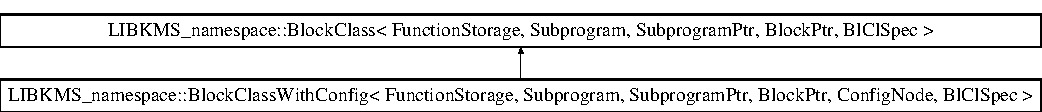
\includegraphics[height=1.499331cm]{classLIBKMS__namespace_1_1BlockClass}
\end{center}
\end{figure}
\subsection*{Открытые типы}
\begin{DoxyCompactItemize}
\item 
typedef \hyperlink{classLIBKMS__namespace_1_1BlockClass}{Block\-Class}\\*
$<$ \hyperlink{classLIBKMS__namespace_1_1FunctionStorage}{Function\-Storage}, \hyperlink{classLIBKMS__namespace_1_1Subprogram}{Subprogram}, \\*
Subprogram\-Ptr, Block\-Ptr, \\*
Bl\-Cl\-Spec $>$ \hyperlink{classLIBKMS__namespace_1_1BlockClass_a505cb3abde8bf16a22913254fe5236a8}{block\-\_\-class\-\_\-t}
\item 
typedef Bl\-Cl\-Spec\\*
$<$ \hyperlink{classLIBKMS__namespace_1_1BlockClass_a505cb3abde8bf16a22913254fe5236a8}{block\-\_\-class\-\_\-t} $>$\-::ptr \hyperlink{classLIBKMS__namespace_1_1BlockClass_a37593e298865c9e7050501f7ef176c91}{ptr\-\_\-t}
\item 
typedef \\*
\hyperlink{classLIBKMS__namespace_1_1FunctionStorage_a82b240ff1d5e266642cadfdebd37dfa2}{Function\-Storage\-::parameter\-\_\-map} \hyperlink{classLIBKMS__namespace_1_1BlockClass_a3cd7da1e7c30b9f047e99b6c1c433ff4}{parameter\-\_\-map}
\end{DoxyCompactItemize}
\subsection*{Открытые члены}
\begin{DoxyCompactItemize}
\item 
\hyperlink{classLIBKMS__namespace_1_1BlockClass_a7992caf06a72d7f17240e5e24eab61c2}{Block\-Class} (const std\-::string \&subpr\-\_\-name)
\item 
virtual \hyperlink{classLIBKMS__namespace_1_1BlockClass_a1d886c2451ceb0ebc568ca194248f82f}{$\sim$\-Block\-Class} ()
\item 
std\-::string \hyperlink{classLIBKMS__namespace_1_1BlockClass_a782a534ee4e5b4b6a4c49ef2e1094c9b}{get\-\_\-subprog\-\_\-name} ()
\begin{DoxyCompactList}\small\item\em Возвращает имя подпрограммы, определенной для класса блока \end{DoxyCompactList}\item 
virtual bool \hyperlink{classLIBKMS__namespace_1_1BlockClass_a80b37764d473f2072c44a2fcde530b0d}{join\-\_\-with\-\_\-block} (const Block\-Ptr \&bl, const std\-::string \&suffix=\char`\"{}\char`\"{})
\begin{DoxyCompactList}\small\item\em Проверить, все ли необходимые данные есть в блоке \end{DoxyCompactList}\item 
std\-::string \hyperlink{classLIBKMS__namespace_1_1BlockClass_ae0ec4d88f144059e65872b189bda5be5}{get\-\_\-error\-\_\-msg} ()
\begin{DoxyCompactList}\small\item\em Вернуть список сообщений об ошибках \end{DoxyCompactList}\item 
bool \hyperlink{classLIBKMS__namespace_1_1BlockClass_a3be106b0c2ea94a56a621823280e7c3c}{has\-\_\-errors} ()
\item 
virtual \hyperlink{classLIBKMS__namespace_1_1BlockClass_a37593e298865c9e7050501f7ef176c91}{ptr\-\_\-t} \hyperlink{classLIBKMS__namespace_1_1BlockClass_a85199e54635541f20d262fa915140e53}{clone} () const =0
\end{DoxyCompactItemize}
\subsection*{Защищенные члены}
\begin{DoxyCompactItemize}
\item 
virtual Subprogram\-Ptr \hyperlink{classLIBKMS__namespace_1_1BlockClass_abc277736d9a2dd4eabea3c737b027682}{get\-\_\-subprog} (const std\-::string \&)=0
\begin{DoxyCompactList}\small\item\em Возвращает объект-\/подпрограмму для блока \end{DoxyCompactList}\item 
Subprogram\-Ptr \hyperlink{classLIBKMS__namespace_1_1BlockClass_a173ced5accd8f44d49741583c59d3cf6}{construct\-\_\-subprog} (const typename \hyperlink{classLIBKMS__namespace_1_1FunctionStorage_a0319ecd6e0ca02ee509c5f6b6edeb072}{Function\-Storage\-::function\-\_\-t} \&f, const std\-::string \&suffix=\char`\"{}\char`\"{}, double priority=std\-::numeric\-\_\-limits$<$ double $>$\-::max()) noexcept
\item 
void \hyperlink{classLIBKMS__namespace_1_1BlockClass_a451efd541327bb76ec4aaa1037c5a9da}{set\-\_\-error\-\_\-msg} (const std\-::string \&s)
\begin{DoxyCompactList}\small\item\em Установить сообщение об ошибке \end{DoxyCompactList}\item 
void \hyperlink{classLIBKMS__namespace_1_1BlockClass_ada0b765d7e9db7966c55469de098c2d9}{add\-\_\-error\-\_\-msg} (const std\-::string \&s)
\begin{DoxyCompactList}\small\item\em Добавить сообщение об ошибке \end{DoxyCompactList}\item 
bool \hyperlink{classLIBKMS__namespace_1_1BlockClass_abff04bac1fc3b2c50f9afe056d8aa33d}{validate\-\_\-n\-\_\-add\-\_\-var} (const Block\-Ptr \&bl, const std\-::string \&name)
\begin{DoxyCompactList}\small\item\em Проверить, есть ли переменная в блоке и добавить ее в список своих \end{DoxyCompactList}\end{DoxyCompactItemize}
\subsection*{Защищенные данные}
\begin{DoxyCompactItemize}
\item 
\hyperlink{classLIBKMS__namespace_1_1BlockClass_a3cd7da1e7c30b9f047e99b6c1c433ff4}{parameter\-\_\-map} \hyperlink{classLIBKMS__namespace_1_1BlockClass_a67c59fc343b2a7b7b54ab36c55f38484}{\-\_\-vars}
\end{DoxyCompactItemize}


\subsection{Подробное описание}
\subsubsection*{template$<$typename Function\-Storage, typename Subprogram, typename Subprogram\-Ptr, typename Block\-Ptr, template$<$ typename T $>$ class Bl\-Cl\-Spec$>$class L\-I\-B\-K\-M\-S\-\_\-namespace\-::\-Block\-Class$<$ Function\-Storage, Subprogram, Subprogram\-Ptr, Block\-Ptr, Bl\-Cl\-Spec $>$}

Прототип описания класса блока 

Класс блока определяет подпрограмму (subprogram\-\_\-t), вызываемую вместе с блоком.

Подпрограмма должна добавляться в хранилище подпрограмм автоматически при считывании конфигурации с именем, определенном в классе-\/наследнике. Подпрограмма возвращает словарь переменных, которые могут использоваться или не использоваться в блоке. Для добавления действующей функции подпрограммы в хранилище использовать метод add\-\_\-func(...). 

\subsection{Определения типов}
\hypertarget{classLIBKMS__namespace_1_1BlockClass_a505cb3abde8bf16a22913254fe5236a8}{\index{L\-I\-B\-K\-M\-S\-\_\-namespace\-::\-Block\-Class@{L\-I\-B\-K\-M\-S\-\_\-namespace\-::\-Block\-Class}!block\-\_\-class\-\_\-t@{block\-\_\-class\-\_\-t}}
\index{block\-\_\-class\-\_\-t@{block\-\_\-class\-\_\-t}!LIBKMS_namespace::BlockClass@{L\-I\-B\-K\-M\-S\-\_\-namespace\-::\-Block\-Class}}
\subsubsection[{block\-\_\-class\-\_\-t}]{\setlength{\rightskip}{0pt plus 5cm}template$<$typename Function\-Storage , typename Subprogram , typename Subprogram\-Ptr , typename Block\-Ptr , template$<$ typename T $>$ class Bl\-Cl\-Spec$>$ typedef {\bf Block\-Class}$<$ {\bf Function\-Storage}, {\bf Subprogram}, Subprogram\-Ptr, Block\-Ptr, Bl\-Cl\-Spec $>$ {\bf L\-I\-B\-K\-M\-S\-\_\-namespace\-::\-Block\-Class}$<$ {\bf Function\-Storage}, {\bf Subprogram}, Subprogram\-Ptr, Block\-Ptr, Bl\-Cl\-Spec $>$\-::{\bf block\-\_\-class\-\_\-t}}}\label{classLIBKMS__namespace_1_1BlockClass_a505cb3abde8bf16a22913254fe5236a8}
\hypertarget{classLIBKMS__namespace_1_1BlockClass_a3cd7da1e7c30b9f047e99b6c1c433ff4}{\index{L\-I\-B\-K\-M\-S\-\_\-namespace\-::\-Block\-Class@{L\-I\-B\-K\-M\-S\-\_\-namespace\-::\-Block\-Class}!parameter\-\_\-map@{parameter\-\_\-map}}
\index{parameter\-\_\-map@{parameter\-\_\-map}!LIBKMS_namespace::BlockClass@{L\-I\-B\-K\-M\-S\-\_\-namespace\-::\-Block\-Class}}
\subsubsection[{parameter\-\_\-map}]{\setlength{\rightskip}{0pt plus 5cm}template$<$typename Function\-Storage , typename Subprogram , typename Subprogram\-Ptr , typename Block\-Ptr , template$<$ typename T $>$ class Bl\-Cl\-Spec$>$ typedef {\bf Function\-Storage\-::parameter\-\_\-map} {\bf L\-I\-B\-K\-M\-S\-\_\-namespace\-::\-Block\-Class}$<$ {\bf Function\-Storage}, {\bf Subprogram}, Subprogram\-Ptr, Block\-Ptr, Bl\-Cl\-Spec $>$\-::{\bf parameter\-\_\-map}}}\label{classLIBKMS__namespace_1_1BlockClass_a3cd7da1e7c30b9f047e99b6c1c433ff4}
\hypertarget{classLIBKMS__namespace_1_1BlockClass_a37593e298865c9e7050501f7ef176c91}{\index{L\-I\-B\-K\-M\-S\-\_\-namespace\-::\-Block\-Class@{L\-I\-B\-K\-M\-S\-\_\-namespace\-::\-Block\-Class}!ptr\-\_\-t@{ptr\-\_\-t}}
\index{ptr\-\_\-t@{ptr\-\_\-t}!LIBKMS_namespace::BlockClass@{L\-I\-B\-K\-M\-S\-\_\-namespace\-::\-Block\-Class}}
\subsubsection[{ptr\-\_\-t}]{\setlength{\rightskip}{0pt plus 5cm}template$<$typename Function\-Storage , typename Subprogram , typename Subprogram\-Ptr , typename Block\-Ptr , template$<$ typename T $>$ class Bl\-Cl\-Spec$>$ typedef Bl\-Cl\-Spec$<$ {\bf block\-\_\-class\-\_\-t} $>$\-::ptr {\bf L\-I\-B\-K\-M\-S\-\_\-namespace\-::\-Block\-Class}$<$ {\bf Function\-Storage}, {\bf Subprogram}, Subprogram\-Ptr, Block\-Ptr, Bl\-Cl\-Spec $>$\-::{\bf ptr\-\_\-t}}}\label{classLIBKMS__namespace_1_1BlockClass_a37593e298865c9e7050501f7ef176c91}


\subsection{Конструктор(ы)}
\hypertarget{classLIBKMS__namespace_1_1BlockClass_a7992caf06a72d7f17240e5e24eab61c2}{\index{L\-I\-B\-K\-M\-S\-\_\-namespace\-::\-Block\-Class@{L\-I\-B\-K\-M\-S\-\_\-namespace\-::\-Block\-Class}!Block\-Class@{Block\-Class}}
\index{Block\-Class@{Block\-Class}!LIBKMS_namespace::BlockClass@{L\-I\-B\-K\-M\-S\-\_\-namespace\-::\-Block\-Class}}
\subsubsection[{Block\-Class}]{\setlength{\rightskip}{0pt plus 5cm}template$<$typename Function\-Storage , typename Subprogram , typename Subprogram\-Ptr , typename Block\-Ptr , template$<$ typename T $>$ class Bl\-Cl\-Spec$>$ {\bf L\-I\-B\-K\-M\-S\-\_\-namespace\-::\-Block\-Class}$<$ {\bf Function\-Storage}, {\bf Subprogram}, Subprogram\-Ptr, Block\-Ptr, Bl\-Cl\-Spec $>$\-::{\bf Block\-Class} (
\begin{DoxyParamCaption}
\item[{const std\-::string \&}]{subpr\-\_\-name}
\end{DoxyParamCaption}
)\hspace{0.3cm}{\ttfamily [inline]}}}\label{classLIBKMS__namespace_1_1BlockClass_a7992caf06a72d7f17240e5e24eab61c2}
\hypertarget{classLIBKMS__namespace_1_1BlockClass_a1d886c2451ceb0ebc568ca194248f82f}{\index{L\-I\-B\-K\-M\-S\-\_\-namespace\-::\-Block\-Class@{L\-I\-B\-K\-M\-S\-\_\-namespace\-::\-Block\-Class}!$\sim$\-Block\-Class@{$\sim$\-Block\-Class}}
\index{$\sim$\-Block\-Class@{$\sim$\-Block\-Class}!LIBKMS_namespace::BlockClass@{L\-I\-B\-K\-M\-S\-\_\-namespace\-::\-Block\-Class}}
\subsubsection[{$\sim$\-Block\-Class}]{\setlength{\rightskip}{0pt plus 5cm}template$<$typename Function\-Storage , typename Subprogram , typename Subprogram\-Ptr , typename Block\-Ptr , template$<$ typename T $>$ class Bl\-Cl\-Spec$>$ virtual {\bf L\-I\-B\-K\-M\-S\-\_\-namespace\-::\-Block\-Class}$<$ {\bf Function\-Storage}, {\bf Subprogram}, Subprogram\-Ptr, Block\-Ptr, Bl\-Cl\-Spec $>$\-::$\sim${\bf Block\-Class} (
\begin{DoxyParamCaption}
{}
\end{DoxyParamCaption}
)\hspace{0.3cm}{\ttfamily [inline]}, {\ttfamily [virtual]}}}\label{classLIBKMS__namespace_1_1BlockClass_a1d886c2451ceb0ebc568ca194248f82f}


\subsection{Методы}
\hypertarget{classLIBKMS__namespace_1_1BlockClass_ada0b765d7e9db7966c55469de098c2d9}{\index{L\-I\-B\-K\-M\-S\-\_\-namespace\-::\-Block\-Class@{L\-I\-B\-K\-M\-S\-\_\-namespace\-::\-Block\-Class}!add\-\_\-error\-\_\-msg@{add\-\_\-error\-\_\-msg}}
\index{add\-\_\-error\-\_\-msg@{add\-\_\-error\-\_\-msg}!LIBKMS_namespace::BlockClass@{L\-I\-B\-K\-M\-S\-\_\-namespace\-::\-Block\-Class}}
\subsubsection[{add\-\_\-error\-\_\-msg}]{\setlength{\rightskip}{0pt plus 5cm}template$<$typename Function\-Storage , typename Subprogram , typename Subprogram\-Ptr , typename Block\-Ptr , template$<$ typename T $>$ class Bl\-Cl\-Spec$>$ void {\bf L\-I\-B\-K\-M\-S\-\_\-namespace\-::\-Block\-Class}$<$ {\bf Function\-Storage}, {\bf Subprogram}, Subprogram\-Ptr, Block\-Ptr, Bl\-Cl\-Spec $>$\-::add\-\_\-error\-\_\-msg (
\begin{DoxyParamCaption}
\item[{const std\-::string \&}]{s}
\end{DoxyParamCaption}
)\hspace{0.3cm}{\ttfamily [inline]}, {\ttfamily [protected]}}}\label{classLIBKMS__namespace_1_1BlockClass_ada0b765d7e9db7966c55469de098c2d9}


Добавить сообщение об ошибке 

\hypertarget{classLIBKMS__namespace_1_1BlockClass_a85199e54635541f20d262fa915140e53}{\index{L\-I\-B\-K\-M\-S\-\_\-namespace\-::\-Block\-Class@{L\-I\-B\-K\-M\-S\-\_\-namespace\-::\-Block\-Class}!clone@{clone}}
\index{clone@{clone}!LIBKMS_namespace::BlockClass@{L\-I\-B\-K\-M\-S\-\_\-namespace\-::\-Block\-Class}}
\subsubsection[{clone}]{\setlength{\rightskip}{0pt plus 5cm}template$<$typename Function\-Storage , typename Subprogram , typename Subprogram\-Ptr , typename Block\-Ptr , template$<$ typename T $>$ class Bl\-Cl\-Spec$>$ virtual {\bf ptr\-\_\-t} {\bf L\-I\-B\-K\-M\-S\-\_\-namespace\-::\-Block\-Class}$<$ {\bf Function\-Storage}, {\bf Subprogram}, Subprogram\-Ptr, Block\-Ptr, Bl\-Cl\-Spec $>$\-::clone (
\begin{DoxyParamCaption}
{}
\end{DoxyParamCaption}
) const\hspace{0.3cm}{\ttfamily [pure virtual]}}}\label{classLIBKMS__namespace_1_1BlockClass_a85199e54635541f20d262fa915140e53}
\hypertarget{classLIBKMS__namespace_1_1BlockClass_a173ced5accd8f44d49741583c59d3cf6}{\index{L\-I\-B\-K\-M\-S\-\_\-namespace\-::\-Block\-Class@{L\-I\-B\-K\-M\-S\-\_\-namespace\-::\-Block\-Class}!construct\-\_\-subprog@{construct\-\_\-subprog}}
\index{construct\-\_\-subprog@{construct\-\_\-subprog}!LIBKMS_namespace::BlockClass@{L\-I\-B\-K\-M\-S\-\_\-namespace\-::\-Block\-Class}}
\subsubsection[{construct\-\_\-subprog}]{\setlength{\rightskip}{0pt plus 5cm}template$<$typename Function\-Storage , typename Subprogram , typename Subprogram\-Ptr , typename Block\-Ptr , template$<$ typename T $>$ class Bl\-Cl\-Spec$>$ Subprogram\-Ptr {\bf L\-I\-B\-K\-M\-S\-\_\-namespace\-::\-Block\-Class}$<$ {\bf Function\-Storage}, {\bf Subprogram}, Subprogram\-Ptr, Block\-Ptr, Bl\-Cl\-Spec $>$\-::construct\-\_\-subprog (
\begin{DoxyParamCaption}
\item[{const typename {\bf Function\-Storage\-::function\-\_\-t} \&}]{f, }
\item[{const std\-::string \&}]{suffix = {\ttfamily \char`\"{}\char`\"{}}, }
\item[{double}]{priority = {\ttfamily std\-:\-:numeric\-\_\-limits$<$~double~$>$\-:\-:max()}}
\end{DoxyParamCaption}
)\hspace{0.3cm}{\ttfamily [inline]}, {\ttfamily [protected]}, {\ttfamily [noexcept]}}}\label{classLIBKMS__namespace_1_1BlockClass_a173ced5accd8f44d49741583c59d3cf6}
Сформировать и вернуть указатель на подпрограмму \begin{DoxyNote}{Заметки}
Для одного и того же класса блока в зависимости от конфигурации могут быть определены различные функции, поэтому требуется суффикс к имени функции add. 
\end{DoxyNote}

\begin{DoxyParams}{Аргументы}
{\em add} & суффикс к имени функции \\
\hline
{\em f} & функция, которая будет положена в хранилище и использована в подпрограмме \\
\hline
\end{DoxyParams}
\hypertarget{classLIBKMS__namespace_1_1BlockClass_ae0ec4d88f144059e65872b189bda5be5}{\index{L\-I\-B\-K\-M\-S\-\_\-namespace\-::\-Block\-Class@{L\-I\-B\-K\-M\-S\-\_\-namespace\-::\-Block\-Class}!get\-\_\-error\-\_\-msg@{get\-\_\-error\-\_\-msg}}
\index{get\-\_\-error\-\_\-msg@{get\-\_\-error\-\_\-msg}!LIBKMS_namespace::BlockClass@{L\-I\-B\-K\-M\-S\-\_\-namespace\-::\-Block\-Class}}
\subsubsection[{get\-\_\-error\-\_\-msg}]{\setlength{\rightskip}{0pt plus 5cm}template$<$typename Function\-Storage , typename Subprogram , typename Subprogram\-Ptr , typename Block\-Ptr , template$<$ typename T $>$ class Bl\-Cl\-Spec$>$ std\-::string {\bf L\-I\-B\-K\-M\-S\-\_\-namespace\-::\-Block\-Class}$<$ {\bf Function\-Storage}, {\bf Subprogram}, Subprogram\-Ptr, Block\-Ptr, Bl\-Cl\-Spec $>$\-::get\-\_\-error\-\_\-msg (
\begin{DoxyParamCaption}
{}
\end{DoxyParamCaption}
)\hspace{0.3cm}{\ttfamily [inline]}}}\label{classLIBKMS__namespace_1_1BlockClass_ae0ec4d88f144059e65872b189bda5be5}


Вернуть список сообщений об ошибках 

\hypertarget{classLIBKMS__namespace_1_1BlockClass_abc277736d9a2dd4eabea3c737b027682}{\index{L\-I\-B\-K\-M\-S\-\_\-namespace\-::\-Block\-Class@{L\-I\-B\-K\-M\-S\-\_\-namespace\-::\-Block\-Class}!get\-\_\-subprog@{get\-\_\-subprog}}
\index{get\-\_\-subprog@{get\-\_\-subprog}!LIBKMS_namespace::BlockClass@{L\-I\-B\-K\-M\-S\-\_\-namespace\-::\-Block\-Class}}
\subsubsection[{get\-\_\-subprog}]{\setlength{\rightskip}{0pt plus 5cm}template$<$typename Function\-Storage , typename Subprogram , typename Subprogram\-Ptr , typename Block\-Ptr , template$<$ typename T $>$ class Bl\-Cl\-Spec$>$ virtual Subprogram\-Ptr {\bf L\-I\-B\-K\-M\-S\-\_\-namespace\-::\-Block\-Class}$<$ {\bf Function\-Storage}, {\bf Subprogram}, Subprogram\-Ptr, Block\-Ptr, Bl\-Cl\-Spec $>$\-::get\-\_\-subprog (
\begin{DoxyParamCaption}
\item[{const std\-::string \&}]{}
\end{DoxyParamCaption}
)\hspace{0.3cm}{\ttfamily [protected]}, {\ttfamily [pure virtual]}}}\label{classLIBKMS__namespace_1_1BlockClass_abc277736d9a2dd4eabea3c737b027682}


Возвращает объект-\/подпрограмму для блока 



Замещается в \hyperlink{structLIBKMS__namespace_1_1BlockClassWithConfig_af747a8a47b472e9ef2e8a45ab925c4f1}{L\-I\-B\-K\-M\-S\-\_\-namespace\-::\-Block\-Class\-With\-Config$<$ Function\-Storage, Subprogram, Subprogram\-Ptr, Block\-Ptr, Config\-Node, Bl\-Cl\-Spec $>$}.

\hypertarget{classLIBKMS__namespace_1_1BlockClass_a782a534ee4e5b4b6a4c49ef2e1094c9b}{\index{L\-I\-B\-K\-M\-S\-\_\-namespace\-::\-Block\-Class@{L\-I\-B\-K\-M\-S\-\_\-namespace\-::\-Block\-Class}!get\-\_\-subprog\-\_\-name@{get\-\_\-subprog\-\_\-name}}
\index{get\-\_\-subprog\-\_\-name@{get\-\_\-subprog\-\_\-name}!LIBKMS_namespace::BlockClass@{L\-I\-B\-K\-M\-S\-\_\-namespace\-::\-Block\-Class}}
\subsubsection[{get\-\_\-subprog\-\_\-name}]{\setlength{\rightskip}{0pt plus 5cm}template$<$typename Function\-Storage , typename Subprogram , typename Subprogram\-Ptr , typename Block\-Ptr , template$<$ typename T $>$ class Bl\-Cl\-Spec$>$ std\-::string {\bf L\-I\-B\-K\-M\-S\-\_\-namespace\-::\-Block\-Class}$<$ {\bf Function\-Storage}, {\bf Subprogram}, Subprogram\-Ptr, Block\-Ptr, Bl\-Cl\-Spec $>$\-::get\-\_\-subprog\-\_\-name (
\begin{DoxyParamCaption}
{}
\end{DoxyParamCaption}
)\hspace{0.3cm}{\ttfamily [inline]}}}\label{classLIBKMS__namespace_1_1BlockClass_a782a534ee4e5b4b6a4c49ef2e1094c9b}


Возвращает имя подпрограммы, определенной для класса блока 

\hypertarget{classLIBKMS__namespace_1_1BlockClass_a3be106b0c2ea94a56a621823280e7c3c}{\index{L\-I\-B\-K\-M\-S\-\_\-namespace\-::\-Block\-Class@{L\-I\-B\-K\-M\-S\-\_\-namespace\-::\-Block\-Class}!has\-\_\-errors@{has\-\_\-errors}}
\index{has\-\_\-errors@{has\-\_\-errors}!LIBKMS_namespace::BlockClass@{L\-I\-B\-K\-M\-S\-\_\-namespace\-::\-Block\-Class}}
\subsubsection[{has\-\_\-errors}]{\setlength{\rightskip}{0pt plus 5cm}template$<$typename Function\-Storage , typename Subprogram , typename Subprogram\-Ptr , typename Block\-Ptr , template$<$ typename T $>$ class Bl\-Cl\-Spec$>$ bool {\bf L\-I\-B\-K\-M\-S\-\_\-namespace\-::\-Block\-Class}$<$ {\bf Function\-Storage}, {\bf Subprogram}, Subprogram\-Ptr, Block\-Ptr, Bl\-Cl\-Spec $>$\-::has\-\_\-errors (
\begin{DoxyParamCaption}
{}
\end{DoxyParamCaption}
)\hspace{0.3cm}{\ttfamily [inline]}}}\label{classLIBKMS__namespace_1_1BlockClass_a3be106b0c2ea94a56a621823280e7c3c}
\hypertarget{classLIBKMS__namespace_1_1BlockClass_a80b37764d473f2072c44a2fcde530b0d}{\index{L\-I\-B\-K\-M\-S\-\_\-namespace\-::\-Block\-Class@{L\-I\-B\-K\-M\-S\-\_\-namespace\-::\-Block\-Class}!join\-\_\-with\-\_\-block@{join\-\_\-with\-\_\-block}}
\index{join\-\_\-with\-\_\-block@{join\-\_\-with\-\_\-block}!LIBKMS_namespace::BlockClass@{L\-I\-B\-K\-M\-S\-\_\-namespace\-::\-Block\-Class}}
\subsubsection[{join\-\_\-with\-\_\-block}]{\setlength{\rightskip}{0pt plus 5cm}template$<$typename Function\-Storage , typename Subprogram , typename Subprogram\-Ptr , typename Block\-Ptr , template$<$ typename T $>$ class Bl\-Cl\-Spec$>$ virtual bool {\bf L\-I\-B\-K\-M\-S\-\_\-namespace\-::\-Block\-Class}$<$ {\bf Function\-Storage}, {\bf Subprogram}, Subprogram\-Ptr, Block\-Ptr, Bl\-Cl\-Spec $>$\-::join\-\_\-with\-\_\-block (
\begin{DoxyParamCaption}
\item[{const Block\-Ptr \&}]{bl, }
\item[{const std\-::string \&}]{suffix = {\ttfamily \char`\"{}\char`\"{}}}
\end{DoxyParamCaption}
)\hspace{0.3cm}{\ttfamily [inline]}, {\ttfamily [virtual]}}}\label{classLIBKMS__namespace_1_1BlockClass_a80b37764d473f2072c44a2fcde530b0d}


Проверить, все ли необходимые данные есть в блоке 

\hypertarget{classLIBKMS__namespace_1_1BlockClass_a451efd541327bb76ec4aaa1037c5a9da}{\index{L\-I\-B\-K\-M\-S\-\_\-namespace\-::\-Block\-Class@{L\-I\-B\-K\-M\-S\-\_\-namespace\-::\-Block\-Class}!set\-\_\-error\-\_\-msg@{set\-\_\-error\-\_\-msg}}
\index{set\-\_\-error\-\_\-msg@{set\-\_\-error\-\_\-msg}!LIBKMS_namespace::BlockClass@{L\-I\-B\-K\-M\-S\-\_\-namespace\-::\-Block\-Class}}
\subsubsection[{set\-\_\-error\-\_\-msg}]{\setlength{\rightskip}{0pt plus 5cm}template$<$typename Function\-Storage , typename Subprogram , typename Subprogram\-Ptr , typename Block\-Ptr , template$<$ typename T $>$ class Bl\-Cl\-Spec$>$ void {\bf L\-I\-B\-K\-M\-S\-\_\-namespace\-::\-Block\-Class}$<$ {\bf Function\-Storage}, {\bf Subprogram}, Subprogram\-Ptr, Block\-Ptr, Bl\-Cl\-Spec $>$\-::set\-\_\-error\-\_\-msg (
\begin{DoxyParamCaption}
\item[{const std\-::string \&}]{s}
\end{DoxyParamCaption}
)\hspace{0.3cm}{\ttfamily [inline]}, {\ttfamily [protected]}}}\label{classLIBKMS__namespace_1_1BlockClass_a451efd541327bb76ec4aaa1037c5a9da}


Установить сообщение об ошибке 

\hypertarget{classLIBKMS__namespace_1_1BlockClass_abff04bac1fc3b2c50f9afe056d8aa33d}{\index{L\-I\-B\-K\-M\-S\-\_\-namespace\-::\-Block\-Class@{L\-I\-B\-K\-M\-S\-\_\-namespace\-::\-Block\-Class}!validate\-\_\-n\-\_\-add\-\_\-var@{validate\-\_\-n\-\_\-add\-\_\-var}}
\index{validate\-\_\-n\-\_\-add\-\_\-var@{validate\-\_\-n\-\_\-add\-\_\-var}!LIBKMS_namespace::BlockClass@{L\-I\-B\-K\-M\-S\-\_\-namespace\-::\-Block\-Class}}
\subsubsection[{validate\-\_\-n\-\_\-add\-\_\-var}]{\setlength{\rightskip}{0pt plus 5cm}template$<$typename Function\-Storage , typename Subprogram , typename Subprogram\-Ptr , typename Block\-Ptr , template$<$ typename T $>$ class Bl\-Cl\-Spec$>$ bool {\bf L\-I\-B\-K\-M\-S\-\_\-namespace\-::\-Block\-Class}$<$ {\bf Function\-Storage}, {\bf Subprogram}, Subprogram\-Ptr, Block\-Ptr, Bl\-Cl\-Spec $>$\-::validate\-\_\-n\-\_\-add\-\_\-var (
\begin{DoxyParamCaption}
\item[{const Block\-Ptr \&}]{bl, }
\item[{const std\-::string \&}]{name}
\end{DoxyParamCaption}
)\hspace{0.3cm}{\ttfamily [inline]}, {\ttfamily [protected]}}}\label{classLIBKMS__namespace_1_1BlockClass_abff04bac1fc3b2c50f9afe056d8aa33d}


Проверить, есть ли переменная в блоке и добавить ее в список своих 



\subsection{Данные класса}
\hypertarget{classLIBKMS__namespace_1_1BlockClass_a67c59fc343b2a7b7b54ab36c55f38484}{\index{L\-I\-B\-K\-M\-S\-\_\-namespace\-::\-Block\-Class@{L\-I\-B\-K\-M\-S\-\_\-namespace\-::\-Block\-Class}!\-\_\-vars@{\-\_\-vars}}
\index{\-\_\-vars@{\-\_\-vars}!LIBKMS_namespace::BlockClass@{L\-I\-B\-K\-M\-S\-\_\-namespace\-::\-Block\-Class}}
\subsubsection[{\-\_\-vars}]{\setlength{\rightskip}{0pt plus 5cm}template$<$typename Function\-Storage , typename Subprogram , typename Subprogram\-Ptr , typename Block\-Ptr , template$<$ typename T $>$ class Bl\-Cl\-Spec$>$ {\bf parameter\-\_\-map} {\bf L\-I\-B\-K\-M\-S\-\_\-namespace\-::\-Block\-Class}$<$ {\bf Function\-Storage}, {\bf Subprogram}, Subprogram\-Ptr, Block\-Ptr, Bl\-Cl\-Spec $>$\-::\-\_\-vars\hspace{0.3cm}{\ttfamily [protected]}}}\label{classLIBKMS__namespace_1_1BlockClass_a67c59fc343b2a7b7b54ab36c55f38484}


Объявления и описания членов класса находятся в файле\-:\begin{DoxyCompactItemize}
\item 
\hyperlink{block__class_8hpp}{block\-\_\-class.\-hpp}\end{DoxyCompactItemize}

\hypertarget{classLIBKMS__namespace_1_1BlockClassFactory}{\section{Шаблон класса L\-I\-B\-K\-M\-S\-\_\-namespace\-:\-:Block\-Class\-Factory$<$ Function\-Storage, Subprogram, Subprogram\-Ptr, Block\-Ptr, Bl\-Cl\-Spec $>$}
\label{classLIBKMS__namespace_1_1BlockClassFactory}\index{L\-I\-B\-K\-M\-S\-\_\-namespace\-::\-Block\-Class\-Factory$<$ Function\-Storage, Subprogram, Subprogram\-Ptr, Block\-Ptr, Bl\-Cl\-Spec $>$@{L\-I\-B\-K\-M\-S\-\_\-namespace\-::\-Block\-Class\-Factory$<$ Function\-Storage, Subprogram, Subprogram\-Ptr, Block\-Ptr, Bl\-Cl\-Spec $>$}}
}


Фабрика классов блоков  




{\ttfamily \#include $<$block\-\_\-class.\-hpp$>$}

\subsection*{Классы}
\begin{DoxyCompactItemize}
\item 
struct \hyperlink{structLIBKMS__namespace_1_1BlockClassFactory_1_1block__class__with__config}{block\-\_\-class\-\_\-with\-\_\-config}
\end{DoxyCompactItemize}
\subsection*{Открытые типы}
\begin{DoxyCompactItemize}
\item 
typedef \hyperlink{classLIBKMS__namespace_1_1BlockClassFactory}{Block\-Class\-Factory}\\*
$<$ \hyperlink{classLIBKMS__namespace_1_1FunctionStorage}{Function\-Storage}, \hyperlink{classLIBKMS__namespace_1_1Subprogram}{Subprogram}, \\*
Subprogram\-Ptr, Block\-Ptr, \\*
Bl\-Cl\-Spec $>$ \hyperlink{classLIBKMS__namespace_1_1BlockClassFactory_ac764a55036aeecf1279f5b43464ab9ad}{block\-\_\-class\-\_\-factory\-\_\-t}
\item 
typedef \hyperlink{classLIBKMS__namespace_1_1BlockClass}{Block\-Class}\\*
$<$ \hyperlink{classLIBKMS__namespace_1_1FunctionStorage}{Function\-Storage}, \hyperlink{classLIBKMS__namespace_1_1Subprogram}{Subprogram}, \\*
Subprogram\-Ptr, Block\-Ptr, \\*
Bl\-Cl\-Spec $>$ \hyperlink{classLIBKMS__namespace_1_1BlockClassFactory_ab6e704b98791fd6c718cfbb0fe2d2a5a}{block\-\_\-class\-\_\-t}
\item 
typedef Bl\-Cl\-Spec\\*
$<$ \hyperlink{classLIBKMS__namespace_1_1BlockClassFactory_ab6e704b98791fd6c718cfbb0fe2d2a5a}{block\-\_\-class\-\_\-t} $>$\-::ptr \hyperlink{classLIBKMS__namespace_1_1BlockClassFactory_a882880cb8a33fcc808b41e283cea2dc3}{block\-\_\-class\-\_\-ptr}
\item 
typedef Bl\-Cl\-Spec\\*
$<$ \hyperlink{classLIBKMS__namespace_1_1BlockClassFactory_ab6e704b98791fd6c718cfbb0fe2d2a5a}{block\-\_\-class\-\_\-t} $>$\-::map \hyperlink{classLIBKMS__namespace_1_1BlockClassFactory_a6c80887a7827dcc55a3508b242b906c9}{block\-\_\-class\-\_\-map}
\end{DoxyCompactItemize}
\subsection*{Открытые члены}
\begin{DoxyCompactItemize}
\item 
\hyperlink{classLIBKMS__namespace_1_1BlockClassFactory_a882880cb8a33fcc808b41e283cea2dc3}{block\-\_\-class\-\_\-ptr} \hyperlink{classLIBKMS__namespace_1_1BlockClassFactory_a51d6671829d0b5ac15c27adc604835db}{create} (const std\-::string \&classname) const noexcept
\begin{DoxyCompactList}\small\item\em Создать экземпляр класса блока \end{DoxyCompactList}\item 
{\footnotesize template$<$typename T $>$ }\\bool \hyperlink{classLIBKMS__namespace_1_1BlockClassFactory_a185c0b7f022b7dea757e663bac1a1caa}{add\-\_\-block\-\_\-class} (const std\-::string \&classname)
\end{DoxyCompactItemize}
\subsection*{Открытые статические члены}
\begin{DoxyCompactItemize}
\item 
static \hyperlink{classLIBKMS__namespace_1_1BlockClassFactory_ac764a55036aeecf1279f5b43464ab9ad}{block\-\_\-class\-\_\-factory\-\_\-t} \& \hyperlink{classLIBKMS__namespace_1_1BlockClassFactory_a95ef3434b162301444650d201025bca6}{instance} () noexcept
\begin{DoxyCompactList}\small\item\em Вернуть экземпляр фабрики классов блоков \end{DoxyCompactList}\item 
{\footnotesize template$<$typename T $>$ }\\static \hyperlink{structLIBKMS__namespace_1_1BlockClassFactory_1_1block__class__with__config}{block\-\_\-class\-\_\-with\-\_\-config}\\*
$<$ T $>$\-::ptr\-\_\-t \hyperlink{classLIBKMS__namespace_1_1BlockClassFactory_afb4a03e20d36516a2b1ac6c3214bc1d8}{with\-\_\-config} (const \hyperlink{classLIBKMS__namespace_1_1BlockClassFactory_a882880cb8a33fcc808b41e283cea2dc3}{block\-\_\-class\-\_\-ptr} p)
\end{DoxyCompactItemize}


\subsection{Подробное описание}
\subsubsection*{template$<$typename Function\-Storage, typename Subprogram, typename Subprogram\-Ptr, typename Block\-Ptr, template$<$ typename U $>$ class Bl\-Cl\-Spec$>$class L\-I\-B\-K\-M\-S\-\_\-namespace\-::\-Block\-Class\-Factory$<$ Function\-Storage, Subprogram, Subprogram\-Ptr, Block\-Ptr, Bl\-Cl\-Spec $>$}

Фабрика классов блоков 

\subsection{Определения типов}
\hypertarget{classLIBKMS__namespace_1_1BlockClassFactory_ac764a55036aeecf1279f5b43464ab9ad}{\index{L\-I\-B\-K\-M\-S\-\_\-namespace\-::\-Block\-Class\-Factory@{L\-I\-B\-K\-M\-S\-\_\-namespace\-::\-Block\-Class\-Factory}!block\-\_\-class\-\_\-factory\-\_\-t@{block\-\_\-class\-\_\-factory\-\_\-t}}
\index{block\-\_\-class\-\_\-factory\-\_\-t@{block\-\_\-class\-\_\-factory\-\_\-t}!LIBKMS_namespace::BlockClassFactory@{L\-I\-B\-K\-M\-S\-\_\-namespace\-::\-Block\-Class\-Factory}}
\subsubsection[{block\-\_\-class\-\_\-factory\-\_\-t}]{\setlength{\rightskip}{0pt plus 5cm}template$<$typename Function\-Storage , typename Subprogram , typename Subprogram\-Ptr , typename Block\-Ptr , template$<$ typename U $>$ class Bl\-Cl\-Spec$>$ typedef {\bf Block\-Class\-Factory}$<$ {\bf Function\-Storage}, {\bf Subprogram}, Subprogram\-Ptr, Block\-Ptr, Bl\-Cl\-Spec $>$ {\bf L\-I\-B\-K\-M\-S\-\_\-namespace\-::\-Block\-Class\-Factory}$<$ {\bf Function\-Storage}, {\bf Subprogram}, Subprogram\-Ptr, Block\-Ptr, Bl\-Cl\-Spec $>$\-::{\bf block\-\_\-class\-\_\-factory\-\_\-t}}}\label{classLIBKMS__namespace_1_1BlockClassFactory_ac764a55036aeecf1279f5b43464ab9ad}
\hypertarget{classLIBKMS__namespace_1_1BlockClassFactory_a6c80887a7827dcc55a3508b242b906c9}{\index{L\-I\-B\-K\-M\-S\-\_\-namespace\-::\-Block\-Class\-Factory@{L\-I\-B\-K\-M\-S\-\_\-namespace\-::\-Block\-Class\-Factory}!block\-\_\-class\-\_\-map@{block\-\_\-class\-\_\-map}}
\index{block\-\_\-class\-\_\-map@{block\-\_\-class\-\_\-map}!LIBKMS_namespace::BlockClassFactory@{L\-I\-B\-K\-M\-S\-\_\-namespace\-::\-Block\-Class\-Factory}}
\subsubsection[{block\-\_\-class\-\_\-map}]{\setlength{\rightskip}{0pt plus 5cm}template$<$typename Function\-Storage , typename Subprogram , typename Subprogram\-Ptr , typename Block\-Ptr , template$<$ typename U $>$ class Bl\-Cl\-Spec$>$ typedef Bl\-Cl\-Spec$<$ {\bf block\-\_\-class\-\_\-t} $>$\-::map {\bf L\-I\-B\-K\-M\-S\-\_\-namespace\-::\-Block\-Class\-Factory}$<$ {\bf Function\-Storage}, {\bf Subprogram}, Subprogram\-Ptr, Block\-Ptr, Bl\-Cl\-Spec $>$\-::{\bf block\-\_\-class\-\_\-map}}}\label{classLIBKMS__namespace_1_1BlockClassFactory_a6c80887a7827dcc55a3508b242b906c9}
\hypertarget{classLIBKMS__namespace_1_1BlockClassFactory_a882880cb8a33fcc808b41e283cea2dc3}{\index{L\-I\-B\-K\-M\-S\-\_\-namespace\-::\-Block\-Class\-Factory@{L\-I\-B\-K\-M\-S\-\_\-namespace\-::\-Block\-Class\-Factory}!block\-\_\-class\-\_\-ptr@{block\-\_\-class\-\_\-ptr}}
\index{block\-\_\-class\-\_\-ptr@{block\-\_\-class\-\_\-ptr}!LIBKMS_namespace::BlockClassFactory@{L\-I\-B\-K\-M\-S\-\_\-namespace\-::\-Block\-Class\-Factory}}
\subsubsection[{block\-\_\-class\-\_\-ptr}]{\setlength{\rightskip}{0pt plus 5cm}template$<$typename Function\-Storage , typename Subprogram , typename Subprogram\-Ptr , typename Block\-Ptr , template$<$ typename U $>$ class Bl\-Cl\-Spec$>$ typedef Bl\-Cl\-Spec$<$ {\bf block\-\_\-class\-\_\-t} $>$\-::ptr {\bf L\-I\-B\-K\-M\-S\-\_\-namespace\-::\-Block\-Class\-Factory}$<$ {\bf Function\-Storage}, {\bf Subprogram}, Subprogram\-Ptr, Block\-Ptr, Bl\-Cl\-Spec $>$\-::{\bf block\-\_\-class\-\_\-ptr}}}\label{classLIBKMS__namespace_1_1BlockClassFactory_a882880cb8a33fcc808b41e283cea2dc3}
\hypertarget{classLIBKMS__namespace_1_1BlockClassFactory_ab6e704b98791fd6c718cfbb0fe2d2a5a}{\index{L\-I\-B\-K\-M\-S\-\_\-namespace\-::\-Block\-Class\-Factory@{L\-I\-B\-K\-M\-S\-\_\-namespace\-::\-Block\-Class\-Factory}!block\-\_\-class\-\_\-t@{block\-\_\-class\-\_\-t}}
\index{block\-\_\-class\-\_\-t@{block\-\_\-class\-\_\-t}!LIBKMS_namespace::BlockClassFactory@{L\-I\-B\-K\-M\-S\-\_\-namespace\-::\-Block\-Class\-Factory}}
\subsubsection[{block\-\_\-class\-\_\-t}]{\setlength{\rightskip}{0pt plus 5cm}template$<$typename Function\-Storage , typename Subprogram , typename Subprogram\-Ptr , typename Block\-Ptr , template$<$ typename U $>$ class Bl\-Cl\-Spec$>$ typedef {\bf Block\-Class}$<$ {\bf Function\-Storage}, {\bf Subprogram}, Subprogram\-Ptr, Block\-Ptr, Bl\-Cl\-Spec $>$ {\bf L\-I\-B\-K\-M\-S\-\_\-namespace\-::\-Block\-Class\-Factory}$<$ {\bf Function\-Storage}, {\bf Subprogram}, Subprogram\-Ptr, Block\-Ptr, Bl\-Cl\-Spec $>$\-::{\bf block\-\_\-class\-\_\-t}}}\label{classLIBKMS__namespace_1_1BlockClassFactory_ab6e704b98791fd6c718cfbb0fe2d2a5a}


\subsection{Методы}
\hypertarget{classLIBKMS__namespace_1_1BlockClassFactory_a185c0b7f022b7dea757e663bac1a1caa}{\index{L\-I\-B\-K\-M\-S\-\_\-namespace\-::\-Block\-Class\-Factory@{L\-I\-B\-K\-M\-S\-\_\-namespace\-::\-Block\-Class\-Factory}!add\-\_\-block\-\_\-class@{add\-\_\-block\-\_\-class}}
\index{add\-\_\-block\-\_\-class@{add\-\_\-block\-\_\-class}!LIBKMS_namespace::BlockClassFactory@{L\-I\-B\-K\-M\-S\-\_\-namespace\-::\-Block\-Class\-Factory}}
\subsubsection[{add\-\_\-block\-\_\-class}]{\setlength{\rightskip}{0pt plus 5cm}template$<$typename Function\-Storage , typename Subprogram , typename Subprogram\-Ptr , typename Block\-Ptr , template$<$ typename U $>$ class Bl\-Cl\-Spec$>$ template$<$typename T $>$ bool {\bf L\-I\-B\-K\-M\-S\-\_\-namespace\-::\-Block\-Class\-Factory}$<$ {\bf Function\-Storage}, {\bf Subprogram}, Subprogram\-Ptr, Block\-Ptr, Bl\-Cl\-Spec $>$\-::add\-\_\-block\-\_\-class (
\begin{DoxyParamCaption}
\item[{const std\-::string \&}]{classname}
\end{DoxyParamCaption}
)\hspace{0.3cm}{\ttfamily [inline]}}}\label{classLIBKMS__namespace_1_1BlockClassFactory_a185c0b7f022b7dea757e663bac1a1caa}
Добавить новый класс блоков \begin{DoxyReturn}{Возвращает}
добавилось ли 
\end{DoxyReturn}
\hypertarget{classLIBKMS__namespace_1_1BlockClassFactory_a51d6671829d0b5ac15c27adc604835db}{\index{L\-I\-B\-K\-M\-S\-\_\-namespace\-::\-Block\-Class\-Factory@{L\-I\-B\-K\-M\-S\-\_\-namespace\-::\-Block\-Class\-Factory}!create@{create}}
\index{create@{create}!LIBKMS_namespace::BlockClassFactory@{L\-I\-B\-K\-M\-S\-\_\-namespace\-::\-Block\-Class\-Factory}}
\subsubsection[{create}]{\setlength{\rightskip}{0pt plus 5cm}template$<$typename Function\-Storage , typename Subprogram , typename Subprogram\-Ptr , typename Block\-Ptr , template$<$ typename U $>$ class Bl\-Cl\-Spec$>$ {\bf block\-\_\-class\-\_\-ptr} {\bf L\-I\-B\-K\-M\-S\-\_\-namespace\-::\-Block\-Class\-Factory}$<$ {\bf Function\-Storage}, {\bf Subprogram}, Subprogram\-Ptr, Block\-Ptr, Bl\-Cl\-Spec $>$\-::create (
\begin{DoxyParamCaption}
\item[{const std\-::string \&}]{classname}
\end{DoxyParamCaption}
) const\hspace{0.3cm}{\ttfamily [inline]}, {\ttfamily [noexcept]}}}\label{classLIBKMS__namespace_1_1BlockClassFactory_a51d6671829d0b5ac15c27adc604835db}


Создать экземпляр класса блока 

\hypertarget{classLIBKMS__namespace_1_1BlockClassFactory_a95ef3434b162301444650d201025bca6}{\index{L\-I\-B\-K\-M\-S\-\_\-namespace\-::\-Block\-Class\-Factory@{L\-I\-B\-K\-M\-S\-\_\-namespace\-::\-Block\-Class\-Factory}!instance@{instance}}
\index{instance@{instance}!LIBKMS_namespace::BlockClassFactory@{L\-I\-B\-K\-M\-S\-\_\-namespace\-::\-Block\-Class\-Factory}}
\subsubsection[{instance}]{\setlength{\rightskip}{0pt plus 5cm}template$<$typename Function\-Storage , typename Subprogram , typename Subprogram\-Ptr , typename Block\-Ptr , template$<$ typename U $>$ class Bl\-Cl\-Spec$>$ static {\bf block\-\_\-class\-\_\-factory\-\_\-t}\& {\bf L\-I\-B\-K\-M\-S\-\_\-namespace\-::\-Block\-Class\-Factory}$<$ {\bf Function\-Storage}, {\bf Subprogram}, Subprogram\-Ptr, Block\-Ptr, Bl\-Cl\-Spec $>$\-::instance (
\begin{DoxyParamCaption}
{}
\end{DoxyParamCaption}
)\hspace{0.3cm}{\ttfamily [inline]}, {\ttfamily [static]}, {\ttfamily [noexcept]}}}\label{classLIBKMS__namespace_1_1BlockClassFactory_a95ef3434b162301444650d201025bca6}


Вернуть экземпляр фабрики классов блоков 

\hypertarget{classLIBKMS__namespace_1_1BlockClassFactory_afb4a03e20d36516a2b1ac6c3214bc1d8}{\index{L\-I\-B\-K\-M\-S\-\_\-namespace\-::\-Block\-Class\-Factory@{L\-I\-B\-K\-M\-S\-\_\-namespace\-::\-Block\-Class\-Factory}!with\-\_\-config@{with\-\_\-config}}
\index{with\-\_\-config@{with\-\_\-config}!LIBKMS_namespace::BlockClassFactory@{L\-I\-B\-K\-M\-S\-\_\-namespace\-::\-Block\-Class\-Factory}}
\subsubsection[{with\-\_\-config}]{\setlength{\rightskip}{0pt plus 5cm}template$<$typename Function\-Storage , typename Subprogram , typename Subprogram\-Ptr , typename Block\-Ptr , template$<$ typename U $>$ class Bl\-Cl\-Spec$>$ template$<$typename T $>$ static {\bf block\-\_\-class\-\_\-with\-\_\-config}$<$ T $>$\-::ptr\-\_\-t {\bf L\-I\-B\-K\-M\-S\-\_\-namespace\-::\-Block\-Class\-Factory}$<$ {\bf Function\-Storage}, {\bf Subprogram}, Subprogram\-Ptr, Block\-Ptr, Bl\-Cl\-Spec $>$\-::with\-\_\-config (
\begin{DoxyParamCaption}
\item[{const {\bf block\-\_\-class\-\_\-ptr}}]{p}
\end{DoxyParamCaption}
)\hspace{0.3cm}{\ttfamily [inline]}, {\ttfamily [static]}}}\label{classLIBKMS__namespace_1_1BlockClassFactory_afb4a03e20d36516a2b1ac6c3214bc1d8}


Объявления и описания членов класса находятся в файле\-:\begin{DoxyCompactItemize}
\item 
\hyperlink{block__class_8hpp}{block\-\_\-class.\-hpp}\end{DoxyCompactItemize}

\hypertarget{structLIBKMS__namespace_1_1BlockClassWithConfig}{\section{Шаблон структуры L\-I\-B\-K\-M\-S\-\_\-namespace\-:\-:Block\-Class\-With\-Config$<$ Function\-Storage, Subprogram, Subprogram\-Ptr, Block\-Ptr, Config\-Node, Bl\-Cl\-Spec $>$}
\label{structLIBKMS__namespace_1_1BlockClassWithConfig}\index{L\-I\-B\-K\-M\-S\-\_\-namespace\-::\-Block\-Class\-With\-Config$<$ Function\-Storage, Subprogram, Subprogram\-Ptr, Block\-Ptr, Config\-Node, Bl\-Cl\-Spec $>$@{L\-I\-B\-K\-M\-S\-\_\-namespace\-::\-Block\-Class\-With\-Config$<$ Function\-Storage, Subprogram, Subprogram\-Ptr, Block\-Ptr, Config\-Node, Bl\-Cl\-Spec $>$}}
}


{\ttfamily \#include $<$block\-\_\-class.\-hpp$>$}

Граф наследования\-:L\-I\-B\-K\-M\-S\-\_\-namespace\-:\-:Block\-Class\-With\-Config$<$ Function\-Storage, Subprogram, Subprogram\-Ptr, Block\-Ptr, Config\-Node, Bl\-Cl\-Spec $>$\-:\begin{figure}[H]
\begin{center}
\leavevmode
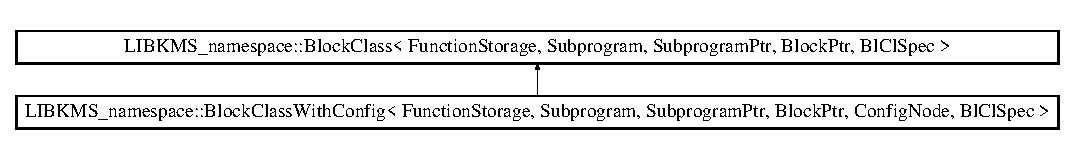
\includegraphics[height=1.499331cm]{structLIBKMS__namespace_1_1BlockClassWithConfig}
\end{center}
\end{figure}
\subsection*{Открытые типы}
\begin{DoxyCompactItemize}
\item 
typedef \hyperlink{classLIBKMS__namespace_1_1BlockClass}{Block\-Class}\\*
$<$ \hyperlink{classLIBKMS__namespace_1_1FunctionStorage}{Function\-Storage}, \hyperlink{classLIBKMS__namespace_1_1Subprogram}{Subprogram}, \\*
Subprogram\-Ptr, Block\-Ptr, \\*
Bl\-Cl\-Spec $>$ \hyperlink{structLIBKMS__namespace_1_1BlockClassWithConfig_a9a90d09b791c08682e6bc111072d87de}{block\-\_\-class\-\_\-t}
\end{DoxyCompactItemize}
\subsection*{Открытые члены}
\begin{DoxyCompactItemize}
\item 
\hyperlink{structLIBKMS__namespace_1_1BlockClassWithConfig_a11cb32afa530052b1fbf4d56cd5610be}{Block\-Class\-With\-Config} (const std\-::string \&subpr\-\_\-name)
\item 
virtual bool \hyperlink{structLIBKMS__namespace_1_1BlockClassWithConfig_a16930c27678eb0887854d6c83f38f301}{read\-\_\-class\-\_\-config} (const Config\-Node \&node)=0
\item 
virtual Subprogram\-Ptr \hyperlink{structLIBKMS__namespace_1_1BlockClassWithConfig_af747a8a47b472e9ef2e8a45ab925c4f1}{get\-\_\-subprog} (const std\-::string \&)=0
\begin{DoxyCompactList}\small\item\em Возвращает объект-\/подпрограмму для блока \end{DoxyCompactList}\end{DoxyCompactItemize}
\subsection*{Дополнительные унаследованные члены}


\subsection{Определения типов}
\hypertarget{structLIBKMS__namespace_1_1BlockClassWithConfig_a9a90d09b791c08682e6bc111072d87de}{\index{L\-I\-B\-K\-M\-S\-\_\-namespace\-::\-Block\-Class\-With\-Config@{L\-I\-B\-K\-M\-S\-\_\-namespace\-::\-Block\-Class\-With\-Config}!block\-\_\-class\-\_\-t@{block\-\_\-class\-\_\-t}}
\index{block\-\_\-class\-\_\-t@{block\-\_\-class\-\_\-t}!LIBKMS_namespace::BlockClassWithConfig@{L\-I\-B\-K\-M\-S\-\_\-namespace\-::\-Block\-Class\-With\-Config}}
\subsubsection[{block\-\_\-class\-\_\-t}]{\setlength{\rightskip}{0pt plus 5cm}template$<$typename Function\-Storage , typename Subprogram , typename Subprogram\-Ptr , typename Block\-Ptr , typename Config\-Node , template$<$ typename U $>$ class Bl\-Cl\-Spec$>$ typedef {\bf Block\-Class}$<$ {\bf Function\-Storage}, {\bf Subprogram}, Subprogram\-Ptr, Block\-Ptr, Bl\-Cl\-Spec $>$ {\bf L\-I\-B\-K\-M\-S\-\_\-namespace\-::\-Block\-Class\-With\-Config}$<$ {\bf Function\-Storage}, {\bf Subprogram}, Subprogram\-Ptr, Block\-Ptr, Config\-Node, Bl\-Cl\-Spec $>$\-::{\bf block\-\_\-class\-\_\-t}}}\label{structLIBKMS__namespace_1_1BlockClassWithConfig_a9a90d09b791c08682e6bc111072d87de}


\subsection{Конструктор(ы)}
\hypertarget{structLIBKMS__namespace_1_1BlockClassWithConfig_a11cb32afa530052b1fbf4d56cd5610be}{\index{L\-I\-B\-K\-M\-S\-\_\-namespace\-::\-Block\-Class\-With\-Config@{L\-I\-B\-K\-M\-S\-\_\-namespace\-::\-Block\-Class\-With\-Config}!Block\-Class\-With\-Config@{Block\-Class\-With\-Config}}
\index{Block\-Class\-With\-Config@{Block\-Class\-With\-Config}!LIBKMS_namespace::BlockClassWithConfig@{L\-I\-B\-K\-M\-S\-\_\-namespace\-::\-Block\-Class\-With\-Config}}
\subsubsection[{Block\-Class\-With\-Config}]{\setlength{\rightskip}{0pt plus 5cm}template$<$typename Function\-Storage , typename Subprogram , typename Subprogram\-Ptr , typename Block\-Ptr , typename Config\-Node , template$<$ typename U $>$ class Bl\-Cl\-Spec$>$ {\bf L\-I\-B\-K\-M\-S\-\_\-namespace\-::\-Block\-Class\-With\-Config}$<$ {\bf Function\-Storage}, {\bf Subprogram}, Subprogram\-Ptr, Block\-Ptr, Config\-Node, Bl\-Cl\-Spec $>$\-::{\bf Block\-Class\-With\-Config} (
\begin{DoxyParamCaption}
\item[{const std\-::string \&}]{subpr\-\_\-name}
\end{DoxyParamCaption}
)\hspace{0.3cm}{\ttfamily [inline]}}}\label{structLIBKMS__namespace_1_1BlockClassWithConfig_a11cb32afa530052b1fbf4d56cd5610be}


\subsection{Методы}
\hypertarget{structLIBKMS__namespace_1_1BlockClassWithConfig_af747a8a47b472e9ef2e8a45ab925c4f1}{\index{L\-I\-B\-K\-M\-S\-\_\-namespace\-::\-Block\-Class\-With\-Config@{L\-I\-B\-K\-M\-S\-\_\-namespace\-::\-Block\-Class\-With\-Config}!get\-\_\-subprog@{get\-\_\-subprog}}
\index{get\-\_\-subprog@{get\-\_\-subprog}!LIBKMS_namespace::BlockClassWithConfig@{L\-I\-B\-K\-M\-S\-\_\-namespace\-::\-Block\-Class\-With\-Config}}
\subsubsection[{get\-\_\-subprog}]{\setlength{\rightskip}{0pt plus 5cm}template$<$typename Function\-Storage , typename Subprogram , typename Subprogram\-Ptr , typename Block\-Ptr , typename Config\-Node , template$<$ typename U $>$ class Bl\-Cl\-Spec$>$ virtual Subprogram\-Ptr {\bf L\-I\-B\-K\-M\-S\-\_\-namespace\-::\-Block\-Class\-With\-Config}$<$ {\bf Function\-Storage}, {\bf Subprogram}, Subprogram\-Ptr, Block\-Ptr, Config\-Node, Bl\-Cl\-Spec $>$\-::get\-\_\-subprog (
\begin{DoxyParamCaption}
\item[{const std\-::string \&}]{}
\end{DoxyParamCaption}
)\hspace{0.3cm}{\ttfamily [pure virtual]}}}\label{structLIBKMS__namespace_1_1BlockClassWithConfig_af747a8a47b472e9ef2e8a45ab925c4f1}


Возвращает объект-\/подпрограмму для блока 



Замещает \hyperlink{classLIBKMS__namespace_1_1BlockClass_abc277736d9a2dd4eabea3c737b027682}{L\-I\-B\-K\-M\-S\-\_\-namespace\-::\-Block\-Class$<$ Function\-Storage, Subprogram, Subprogram\-Ptr, Block\-Ptr, Bl\-Cl\-Spec $>$}.

\hypertarget{structLIBKMS__namespace_1_1BlockClassWithConfig_a16930c27678eb0887854d6c83f38f301}{\index{L\-I\-B\-K\-M\-S\-\_\-namespace\-::\-Block\-Class\-With\-Config@{L\-I\-B\-K\-M\-S\-\_\-namespace\-::\-Block\-Class\-With\-Config}!read\-\_\-class\-\_\-config@{read\-\_\-class\-\_\-config}}
\index{read\-\_\-class\-\_\-config@{read\-\_\-class\-\_\-config}!LIBKMS_namespace::BlockClassWithConfig@{L\-I\-B\-K\-M\-S\-\_\-namespace\-::\-Block\-Class\-With\-Config}}
\subsubsection[{read\-\_\-class\-\_\-config}]{\setlength{\rightskip}{0pt plus 5cm}template$<$typename Function\-Storage , typename Subprogram , typename Subprogram\-Ptr , typename Block\-Ptr , typename Config\-Node , template$<$ typename U $>$ class Bl\-Cl\-Spec$>$ virtual bool {\bf L\-I\-B\-K\-M\-S\-\_\-namespace\-::\-Block\-Class\-With\-Config}$<$ {\bf Function\-Storage}, {\bf Subprogram}, Subprogram\-Ptr, Block\-Ptr, Config\-Node, Bl\-Cl\-Spec $>$\-::read\-\_\-class\-\_\-config (
\begin{DoxyParamCaption}
\item[{const Config\-Node \&}]{node}
\end{DoxyParamCaption}
)\hspace{0.3cm}{\ttfamily [pure virtual]}}}\label{structLIBKMS__namespace_1_1BlockClassWithConfig_a16930c27678eb0887854d6c83f38f301}


Объявления и описания членов структуры находятся в файле\-:\begin{DoxyCompactItemize}
\item 
\hyperlink{block__class_8hpp}{block\-\_\-class.\-hpp}\end{DoxyCompactItemize}

\hypertarget{classLIBKMS__namespace_1_1Callable}{\section{Шаблон класса L\-I\-B\-K\-M\-S\-\_\-namespace\-:\-:Callable$<$ Logger, Parameter\-Map, Formula\-Solver $>$}
\label{classLIBKMS__namespace_1_1Callable}\index{L\-I\-B\-K\-M\-S\-\_\-namespace\-::\-Callable$<$ Logger, Parameter\-Map, Formula\-Solver $>$@{L\-I\-B\-K\-M\-S\-\_\-namespace\-::\-Callable$<$ Logger, Parameter\-Map, Formula\-Solver $>$}}
}


{\ttfamily \#include $<$callable.\-hpp$>$}

Граф наследования\-:L\-I\-B\-K\-M\-S\-\_\-namespace\-:\-:Callable$<$ Logger, Parameter\-Map, Formula\-Solver $>$\-:\begin{figure}[H]
\begin{center}
\leavevmode
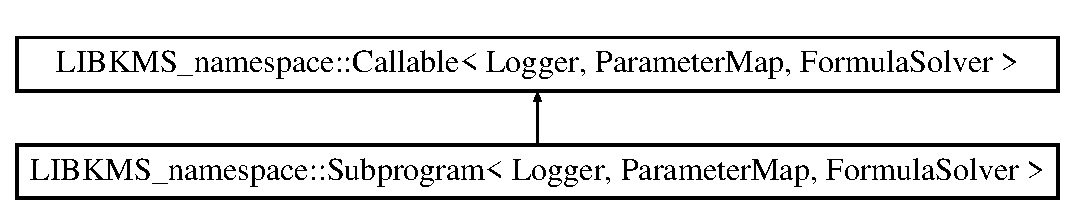
\includegraphics[height=2.000000cm]{classLIBKMS__namespace_1_1Callable}
\end{center}
\end{figure}
\subsection*{Открытые типы}
\begin{DoxyCompactItemize}
\item 
typedef Parameter\-Map \hyperlink{classLIBKMS__namespace_1_1Callable_ad58caabaa5ac247c9d385e6d5451916a}{parameter\-\_\-map}
\end{DoxyCompactItemize}
\subsection*{Открытые члены}
\begin{DoxyCompactItemize}
\item 
\hyperlink{classLIBKMS__namespace_1_1Callable_a2ae113d77b64ace4b5dbc6ac2cb8d22b}{Callable} (std\-::string name, double priority, bool isblocked)
\item 
void \hyperlink{classLIBKMS__namespace_1_1Callable_a3e475788ceb6452ea984ae7c41c173c4}{set\-\_\-name} (std\-::string name)
\item 
std\-::string \hyperlink{classLIBKMS__namespace_1_1Callable_a58a214027a04f1cf8ab9644b9ad57916}{get\-\_\-name} ()
\item 
virtual \hyperlink{classLIBKMS__namespace_1_1Callable_acd80016512d6e1062ae0fe5b4d84776e}{$\sim$\-Callable} ()
\item 
virtual \hyperlink{classLIBKMS__namespace_1_1Callable_ad58caabaa5ac247c9d385e6d5451916a}{parameter\-\_\-map} \hyperlink{classLIBKMS__namespace_1_1Callable_ad9cad480516a054f09c056ae248691b1}{call} (double time, const \hyperlink{classLIBKMS__namespace_1_1Callable_ad58caabaa5ac247c9d385e6d5451916a}{parameter\-\_\-map} \&block\-\_\-vars, const \hyperlink{classLIBKMS__namespace_1_1Callable_ad58caabaa5ac247c9d385e6d5451916a}{parameter\-\_\-map} \&upper\-\_\-vars)=0
\item 
\hyperlink{classLIBKMS__namespace_1_1Callable_ad58caabaa5ac247c9d385e6d5451916a}{parameter\-\_\-map} \hyperlink{classLIBKMS__namespace_1_1Callable_a7838731afe0ac0fee5e88ab64952aa4a}{operator()} (double time, const \hyperlink{classLIBKMS__namespace_1_1Callable_ad58caabaa5ac247c9d385e6d5451916a}{parameter\-\_\-map} \&block\-\_\-vars=no\-\_\-params, const \hyperlink{classLIBKMS__namespace_1_1Callable_ad58caabaa5ac247c9d385e6d5451916a}{parameter\-\_\-map} \&upper\-\_\-vars=no\-\_\-params)
\item 
void \hyperlink{classLIBKMS__namespace_1_1Callable_a300b999c2d5ff9663aeb4cb022a5d79b}{touch} ()
\begin{DoxyCompactList}\small\item\em Запомнить текущее время как время последнего вызова \end{DoxyCompactList}\item 
void \hyperlink{classLIBKMS__namespace_1_1Callable_a42b5186f839fb643c115a7db10b14dbd}{set\-\_\-priority} (double priority) noexcept
\begin{DoxyCompactList}\small\item\em Установить значение приоритета \end{DoxyCompactList}\item 
void \hyperlink{classLIBKMS__namespace_1_1Callable_ad07f298a0831bc06851159003426e199}{set\-\_\-lock} (bool lock) noexcept
\begin{DoxyCompactList}\small\item\em Установить блокировку блока \end{DoxyCompactList}\item 
double \hyperlink{classLIBKMS__namespace_1_1Callable_a43d1d9a56ec6a20d3e47a756a4dea6b2}{get\-\_\-lastcall\-\_\-time} () const noexcept
\item 
double \hyperlink{classLIBKMS__namespace_1_1Callable_aa2668a9d0ec66e3dab36450f3b7c6c5f}{get\-\_\-process\-\_\-time} () const noexcept
\item 
double \hyperlink{classLIBKMS__namespace_1_1Callable_a592eba396f24ff83ce9444027c116d9b}{get\-\_\-delta\-\_\-time} () const noexcept
\item 
double \hyperlink{classLIBKMS__namespace_1_1Callable_afc4d97e5407815e621065af7ce8566d6}{get\-\_\-priority} () const noexcept
\item 
bool \hyperlink{classLIBKMS__namespace_1_1Callable_a7585ce4ee8b17e0a45f40acf784d0229}{is\-\_\-blocked} () const noexcept
\item 
bool \hyperlink{classLIBKMS__namespace_1_1Callable_a07e942cddded27a2b1a7b8eb735904a7}{is\-\_\-powered} (const \hyperlink{classLIBKMS__namespace_1_1Callable_ad58caabaa5ac247c9d385e6d5451916a}{parameter\-\_\-map} \&v) const 
\begin{DoxyCompactList}\small\item\em Является ли объект включенным при заданных входных переменных \end{DoxyCompactList}\item 
bool \hyperlink{classLIBKMS__namespace_1_1Callable_a69c7569651e285a161b243daeca7b2a5}{set\-\_\-power\-\_\-cond} (const std\-::string \&src)
\begin{DoxyCompactList}\small\item\em Считать формулу для определения включения объекта \end{DoxyCompactList}\item 
std\-::string \hyperlink{classLIBKMS__namespace_1_1Callable_a1b5d88ad33daaf0df7168fc125bfda98}{get\-\_\-power\-\_\-cond} () const 
\begin{DoxyCompactList}\small\item\em Вернуть строку с формулой \end{DoxyCompactList}\item 
std\-::vector$<$ std\-::string $>$ \hyperlink{classLIBKMS__namespace_1_1Callable_a3140c543709c0541fee7ef0a6ec23e15}{get\-\_\-power\-\_\-vars} () const 
\begin{DoxyCompactList}\small\item\em Вернуть список переменных \end{DoxyCompactList}\end{DoxyCompactItemize}
\subsection*{Защищенные данные}
\begin{DoxyCompactItemize}
\item 
std\-::string \hyperlink{classLIBKMS__namespace_1_1Callable_a86675c2e858a76fff1431b34d913d6a5}{\-\_\-name}
\item 
double \hyperlink{classLIBKMS__namespace_1_1Callable_a828e2be381cf907c88054e604a17f5a4}{\-\_\-priority}
\item 
bool \hyperlink{classLIBKMS__namespace_1_1Callable_a32c7bfc356667f15d5b40fc2ce41e2f7}{\-\_\-isblocked}
\item 
Formula\-Solver \hyperlink{classLIBKMS__namespace_1_1Callable_a0a2d1ea087e901a7cce848ff0efba7ca}{\-\_\-cond\-\_\-s}
\end{DoxyCompactItemize}


\subsection{Определения типов}
\hypertarget{classLIBKMS__namespace_1_1Callable_ad58caabaa5ac247c9d385e6d5451916a}{\index{L\-I\-B\-K\-M\-S\-\_\-namespace\-::\-Callable@{L\-I\-B\-K\-M\-S\-\_\-namespace\-::\-Callable}!parameter\-\_\-map@{parameter\-\_\-map}}
\index{parameter\-\_\-map@{parameter\-\_\-map}!LIBKMS_namespace::Callable@{L\-I\-B\-K\-M\-S\-\_\-namespace\-::\-Callable}}
\subsubsection[{parameter\-\_\-map}]{\setlength{\rightskip}{0pt plus 5cm}template$<$typename Logger, typename Parameter\-Map, typename Formula\-Solver$>$ typedef Parameter\-Map {\bf L\-I\-B\-K\-M\-S\-\_\-namespace\-::\-Callable}$<$ Logger, Parameter\-Map, Formula\-Solver $>$\-::{\bf parameter\-\_\-map}}}\label{classLIBKMS__namespace_1_1Callable_ad58caabaa5ac247c9d385e6d5451916a}


\subsection{Конструктор(ы)}
\hypertarget{classLIBKMS__namespace_1_1Callable_a2ae113d77b64ace4b5dbc6ac2cb8d22b}{\index{L\-I\-B\-K\-M\-S\-\_\-namespace\-::\-Callable@{L\-I\-B\-K\-M\-S\-\_\-namespace\-::\-Callable}!Callable@{Callable}}
\index{Callable@{Callable}!LIBKMS_namespace::Callable@{L\-I\-B\-K\-M\-S\-\_\-namespace\-::\-Callable}}
\subsubsection[{Callable}]{\setlength{\rightskip}{0pt plus 5cm}template$<$typename Logger, typename Parameter\-Map, typename Formula\-Solver$>$ {\bf L\-I\-B\-K\-M\-S\-\_\-namespace\-::\-Callable}$<$ Logger, Parameter\-Map, Formula\-Solver $>$\-::{\bf Callable} (
\begin{DoxyParamCaption}
\item[{std\-::string}]{name, }
\item[{double}]{priority, }
\item[{bool}]{isblocked}
\end{DoxyParamCaption}
)\hspace{0.3cm}{\ttfamily [inline]}}}\label{classLIBKMS__namespace_1_1Callable_a2ae113d77b64ace4b5dbc6ac2cb8d22b}
\hypertarget{classLIBKMS__namespace_1_1Callable_acd80016512d6e1062ae0fe5b4d84776e}{\index{L\-I\-B\-K\-M\-S\-\_\-namespace\-::\-Callable@{L\-I\-B\-K\-M\-S\-\_\-namespace\-::\-Callable}!$\sim$\-Callable@{$\sim$\-Callable}}
\index{$\sim$\-Callable@{$\sim$\-Callable}!LIBKMS_namespace::Callable@{L\-I\-B\-K\-M\-S\-\_\-namespace\-::\-Callable}}
\subsubsection[{$\sim$\-Callable}]{\setlength{\rightskip}{0pt plus 5cm}template$<$typename Logger, typename Parameter\-Map, typename Formula\-Solver$>$ virtual {\bf L\-I\-B\-K\-M\-S\-\_\-namespace\-::\-Callable}$<$ Logger, Parameter\-Map, Formula\-Solver $>$\-::$\sim${\bf Callable} (
\begin{DoxyParamCaption}
{}
\end{DoxyParamCaption}
)\hspace{0.3cm}{\ttfamily [inline]}, {\ttfamily [virtual]}}}\label{classLIBKMS__namespace_1_1Callable_acd80016512d6e1062ae0fe5b4d84776e}


\subsection{Методы}
\hypertarget{classLIBKMS__namespace_1_1Callable_ad9cad480516a054f09c056ae248691b1}{\index{L\-I\-B\-K\-M\-S\-\_\-namespace\-::\-Callable@{L\-I\-B\-K\-M\-S\-\_\-namespace\-::\-Callable}!call@{call}}
\index{call@{call}!LIBKMS_namespace::Callable@{L\-I\-B\-K\-M\-S\-\_\-namespace\-::\-Callable}}
\subsubsection[{call}]{\setlength{\rightskip}{0pt plus 5cm}template$<$typename Logger, typename Parameter\-Map, typename Formula\-Solver$>$ virtual {\bf parameter\-\_\-map} {\bf L\-I\-B\-K\-M\-S\-\_\-namespace\-::\-Callable}$<$ Logger, Parameter\-Map, Formula\-Solver $>$\-::call (
\begin{DoxyParamCaption}
\item[{double}]{time, }
\item[{const {\bf parameter\-\_\-map} \&}]{block\-\_\-vars, }
\item[{const {\bf parameter\-\_\-map} \&}]{upper\-\_\-vars}
\end{DoxyParamCaption}
)\hspace{0.3cm}{\ttfamily [pure virtual]}}}\label{classLIBKMS__namespace_1_1Callable_ad9cad480516a054f09c056ae248691b1}
Осуществить вызов объекта 
\begin{DoxyParams}{Аргументы}
{\em time} & текущее время \\
\hline
{\em block\-\_\-vars} & переменные родительского блока \\
\hline
{\em upper\-\_\-vars} & переменные родителя родительского блока \\
\hline
\end{DoxyParams}
\begin{DoxyReturn}{Возвращает}
новые значения для переменных родительского блока 
\end{DoxyReturn}


Замещается в \hyperlink{classLIBKMS__namespace_1_1Subprogram_a2898e1d2ff996ca6de8a0d6480be4e1f}{L\-I\-B\-K\-M\-S\-\_\-namespace\-::\-Subprogram$<$ Logger, Parameter\-Map, Formula\-Solver $>$}.

\hypertarget{classLIBKMS__namespace_1_1Callable_a592eba396f24ff83ce9444027c116d9b}{\index{L\-I\-B\-K\-M\-S\-\_\-namespace\-::\-Callable@{L\-I\-B\-K\-M\-S\-\_\-namespace\-::\-Callable}!get\-\_\-delta\-\_\-time@{get\-\_\-delta\-\_\-time}}
\index{get\-\_\-delta\-\_\-time@{get\-\_\-delta\-\_\-time}!LIBKMS_namespace::Callable@{L\-I\-B\-K\-M\-S\-\_\-namespace\-::\-Callable}}
\subsubsection[{get\-\_\-delta\-\_\-time}]{\setlength{\rightskip}{0pt plus 5cm}template$<$typename Logger, typename Parameter\-Map, typename Formula\-Solver$>$ double {\bf L\-I\-B\-K\-M\-S\-\_\-namespace\-::\-Callable}$<$ Logger, Parameter\-Map, Formula\-Solver $>$\-::get\-\_\-delta\-\_\-time (
\begin{DoxyParamCaption}
{}
\end{DoxyParamCaption}
) const\hspace{0.3cm}{\ttfamily [inline]}, {\ttfamily [noexcept]}}}\label{classLIBKMS__namespace_1_1Callable_a592eba396f24ff83ce9444027c116d9b}
\hypertarget{classLIBKMS__namespace_1_1Callable_a43d1d9a56ec6a20d3e47a756a4dea6b2}{\index{L\-I\-B\-K\-M\-S\-\_\-namespace\-::\-Callable@{L\-I\-B\-K\-M\-S\-\_\-namespace\-::\-Callable}!get\-\_\-lastcall\-\_\-time@{get\-\_\-lastcall\-\_\-time}}
\index{get\-\_\-lastcall\-\_\-time@{get\-\_\-lastcall\-\_\-time}!LIBKMS_namespace::Callable@{L\-I\-B\-K\-M\-S\-\_\-namespace\-::\-Callable}}
\subsubsection[{get\-\_\-lastcall\-\_\-time}]{\setlength{\rightskip}{0pt plus 5cm}template$<$typename Logger, typename Parameter\-Map, typename Formula\-Solver$>$ double {\bf L\-I\-B\-K\-M\-S\-\_\-namespace\-::\-Callable}$<$ Logger, Parameter\-Map, Formula\-Solver $>$\-::get\-\_\-lastcall\-\_\-time (
\begin{DoxyParamCaption}
{}
\end{DoxyParamCaption}
) const\hspace{0.3cm}{\ttfamily [inline]}, {\ttfamily [noexcept]}}}\label{classLIBKMS__namespace_1_1Callable_a43d1d9a56ec6a20d3e47a756a4dea6b2}
\hypertarget{classLIBKMS__namespace_1_1Callable_a58a214027a04f1cf8ab9644b9ad57916}{\index{L\-I\-B\-K\-M\-S\-\_\-namespace\-::\-Callable@{L\-I\-B\-K\-M\-S\-\_\-namespace\-::\-Callable}!get\-\_\-name@{get\-\_\-name}}
\index{get\-\_\-name@{get\-\_\-name}!LIBKMS_namespace::Callable@{L\-I\-B\-K\-M\-S\-\_\-namespace\-::\-Callable}}
\subsubsection[{get\-\_\-name}]{\setlength{\rightskip}{0pt plus 5cm}template$<$typename Logger, typename Parameter\-Map, typename Formula\-Solver$>$ std\-::string {\bf L\-I\-B\-K\-M\-S\-\_\-namespace\-::\-Callable}$<$ Logger, Parameter\-Map, Formula\-Solver $>$\-::get\-\_\-name (
\begin{DoxyParamCaption}
{}
\end{DoxyParamCaption}
)\hspace{0.3cm}{\ttfamily [inline]}}}\label{classLIBKMS__namespace_1_1Callable_a58a214027a04f1cf8ab9644b9ad57916}
\hypertarget{classLIBKMS__namespace_1_1Callable_a1b5d88ad33daaf0df7168fc125bfda98}{\index{L\-I\-B\-K\-M\-S\-\_\-namespace\-::\-Callable@{L\-I\-B\-K\-M\-S\-\_\-namespace\-::\-Callable}!get\-\_\-power\-\_\-cond@{get\-\_\-power\-\_\-cond}}
\index{get\-\_\-power\-\_\-cond@{get\-\_\-power\-\_\-cond}!LIBKMS_namespace::Callable@{L\-I\-B\-K\-M\-S\-\_\-namespace\-::\-Callable}}
\subsubsection[{get\-\_\-power\-\_\-cond}]{\setlength{\rightskip}{0pt plus 5cm}template$<$typename Logger, typename Parameter\-Map, typename Formula\-Solver$>$ std\-::string {\bf L\-I\-B\-K\-M\-S\-\_\-namespace\-::\-Callable}$<$ Logger, Parameter\-Map, Formula\-Solver $>$\-::get\-\_\-power\-\_\-cond (
\begin{DoxyParamCaption}
{}
\end{DoxyParamCaption}
) const\hspace{0.3cm}{\ttfamily [inline]}}}\label{classLIBKMS__namespace_1_1Callable_a1b5d88ad33daaf0df7168fc125bfda98}


Вернуть строку с формулой 

\hypertarget{classLIBKMS__namespace_1_1Callable_a3140c543709c0541fee7ef0a6ec23e15}{\index{L\-I\-B\-K\-M\-S\-\_\-namespace\-::\-Callable@{L\-I\-B\-K\-M\-S\-\_\-namespace\-::\-Callable}!get\-\_\-power\-\_\-vars@{get\-\_\-power\-\_\-vars}}
\index{get\-\_\-power\-\_\-vars@{get\-\_\-power\-\_\-vars}!LIBKMS_namespace::Callable@{L\-I\-B\-K\-M\-S\-\_\-namespace\-::\-Callable}}
\subsubsection[{get\-\_\-power\-\_\-vars}]{\setlength{\rightskip}{0pt plus 5cm}template$<$typename Logger, typename Parameter\-Map, typename Formula\-Solver$>$ std\-::vector$<$ std\-::string $>$ {\bf L\-I\-B\-K\-M\-S\-\_\-namespace\-::\-Callable}$<$ Logger, Parameter\-Map, Formula\-Solver $>$\-::get\-\_\-power\-\_\-vars (
\begin{DoxyParamCaption}
{}
\end{DoxyParamCaption}
) const\hspace{0.3cm}{\ttfamily [inline]}}}\label{classLIBKMS__namespace_1_1Callable_a3140c543709c0541fee7ef0a6ec23e15}


Вернуть список переменных 

\hypertarget{classLIBKMS__namespace_1_1Callable_afc4d97e5407815e621065af7ce8566d6}{\index{L\-I\-B\-K\-M\-S\-\_\-namespace\-::\-Callable@{L\-I\-B\-K\-M\-S\-\_\-namespace\-::\-Callable}!get\-\_\-priority@{get\-\_\-priority}}
\index{get\-\_\-priority@{get\-\_\-priority}!LIBKMS_namespace::Callable@{L\-I\-B\-K\-M\-S\-\_\-namespace\-::\-Callable}}
\subsubsection[{get\-\_\-priority}]{\setlength{\rightskip}{0pt plus 5cm}template$<$typename Logger, typename Parameter\-Map, typename Formula\-Solver$>$ double {\bf L\-I\-B\-K\-M\-S\-\_\-namespace\-::\-Callable}$<$ Logger, Parameter\-Map, Formula\-Solver $>$\-::get\-\_\-priority (
\begin{DoxyParamCaption}
{}
\end{DoxyParamCaption}
) const\hspace{0.3cm}{\ttfamily [inline]}, {\ttfamily [noexcept]}}}\label{classLIBKMS__namespace_1_1Callable_afc4d97e5407815e621065af7ce8566d6}
\hypertarget{classLIBKMS__namespace_1_1Callable_aa2668a9d0ec66e3dab36450f3b7c6c5f}{\index{L\-I\-B\-K\-M\-S\-\_\-namespace\-::\-Callable@{L\-I\-B\-K\-M\-S\-\_\-namespace\-::\-Callable}!get\-\_\-process\-\_\-time@{get\-\_\-process\-\_\-time}}
\index{get\-\_\-process\-\_\-time@{get\-\_\-process\-\_\-time}!LIBKMS_namespace::Callable@{L\-I\-B\-K\-M\-S\-\_\-namespace\-::\-Callable}}
\subsubsection[{get\-\_\-process\-\_\-time}]{\setlength{\rightskip}{0pt plus 5cm}template$<$typename Logger, typename Parameter\-Map, typename Formula\-Solver$>$ double {\bf L\-I\-B\-K\-M\-S\-\_\-namespace\-::\-Callable}$<$ Logger, Parameter\-Map, Formula\-Solver $>$\-::get\-\_\-process\-\_\-time (
\begin{DoxyParamCaption}
{}
\end{DoxyParamCaption}
) const\hspace{0.3cm}{\ttfamily [inline]}, {\ttfamily [noexcept]}}}\label{classLIBKMS__namespace_1_1Callable_aa2668a9d0ec66e3dab36450f3b7c6c5f}
\hypertarget{classLIBKMS__namespace_1_1Callable_a7585ce4ee8b17e0a45f40acf784d0229}{\index{L\-I\-B\-K\-M\-S\-\_\-namespace\-::\-Callable@{L\-I\-B\-K\-M\-S\-\_\-namespace\-::\-Callable}!is\-\_\-blocked@{is\-\_\-blocked}}
\index{is\-\_\-blocked@{is\-\_\-blocked}!LIBKMS_namespace::Callable@{L\-I\-B\-K\-M\-S\-\_\-namespace\-::\-Callable}}
\subsubsection[{is\-\_\-blocked}]{\setlength{\rightskip}{0pt plus 5cm}template$<$typename Logger, typename Parameter\-Map, typename Formula\-Solver$>$ bool {\bf L\-I\-B\-K\-M\-S\-\_\-namespace\-::\-Callable}$<$ Logger, Parameter\-Map, Formula\-Solver $>$\-::is\-\_\-blocked (
\begin{DoxyParamCaption}
{}
\end{DoxyParamCaption}
) const\hspace{0.3cm}{\ttfamily [inline]}, {\ttfamily [noexcept]}}}\label{classLIBKMS__namespace_1_1Callable_a7585ce4ee8b17e0a45f40acf784d0229}
\hypertarget{classLIBKMS__namespace_1_1Callable_a07e942cddded27a2b1a7b8eb735904a7}{\index{L\-I\-B\-K\-M\-S\-\_\-namespace\-::\-Callable@{L\-I\-B\-K\-M\-S\-\_\-namespace\-::\-Callable}!is\-\_\-powered@{is\-\_\-powered}}
\index{is\-\_\-powered@{is\-\_\-powered}!LIBKMS_namespace::Callable@{L\-I\-B\-K\-M\-S\-\_\-namespace\-::\-Callable}}
\subsubsection[{is\-\_\-powered}]{\setlength{\rightskip}{0pt plus 5cm}template$<$typename Logger, typename Parameter\-Map, typename Formula\-Solver$>$ bool {\bf L\-I\-B\-K\-M\-S\-\_\-namespace\-::\-Callable}$<$ Logger, Parameter\-Map, Formula\-Solver $>$\-::is\-\_\-powered (
\begin{DoxyParamCaption}
\item[{const {\bf parameter\-\_\-map} \&}]{v}
\end{DoxyParamCaption}
) const\hspace{0.3cm}{\ttfamily [inline]}}}\label{classLIBKMS__namespace_1_1Callable_a07e942cddded27a2b1a7b8eb735904a7}


Является ли объект включенным при заданных входных переменных 

\hypertarget{classLIBKMS__namespace_1_1Callable_a7838731afe0ac0fee5e88ab64952aa4a}{\index{L\-I\-B\-K\-M\-S\-\_\-namespace\-::\-Callable@{L\-I\-B\-K\-M\-S\-\_\-namespace\-::\-Callable}!operator()@{operator()}}
\index{operator()@{operator()}!LIBKMS_namespace::Callable@{L\-I\-B\-K\-M\-S\-\_\-namespace\-::\-Callable}}
\subsubsection[{operator()}]{\setlength{\rightskip}{0pt plus 5cm}template$<$typename Logger, typename Parameter\-Map, typename Formula\-Solver$>$ {\bf parameter\-\_\-map} {\bf L\-I\-B\-K\-M\-S\-\_\-namespace\-::\-Callable}$<$ Logger, Parameter\-Map, Formula\-Solver $>$\-::operator() (
\begin{DoxyParamCaption}
\item[{double}]{time, }
\item[{const {\bf parameter\-\_\-map} \&}]{block\-\_\-vars = {\ttfamily no\-\_\-params}, }
\item[{const {\bf parameter\-\_\-map} \&}]{upper\-\_\-vars = {\ttfamily no\-\_\-params}}
\end{DoxyParamCaption}
)\hspace{0.3cm}{\ttfamily [inline]}}}\label{classLIBKMS__namespace_1_1Callable_a7838731afe0ac0fee5e88ab64952aa4a}
\hypertarget{classLIBKMS__namespace_1_1Callable_ad07f298a0831bc06851159003426e199}{\index{L\-I\-B\-K\-M\-S\-\_\-namespace\-::\-Callable@{L\-I\-B\-K\-M\-S\-\_\-namespace\-::\-Callable}!set\-\_\-lock@{set\-\_\-lock}}
\index{set\-\_\-lock@{set\-\_\-lock}!LIBKMS_namespace::Callable@{L\-I\-B\-K\-M\-S\-\_\-namespace\-::\-Callable}}
\subsubsection[{set\-\_\-lock}]{\setlength{\rightskip}{0pt plus 5cm}template$<$typename Logger, typename Parameter\-Map, typename Formula\-Solver$>$ void {\bf L\-I\-B\-K\-M\-S\-\_\-namespace\-::\-Callable}$<$ Logger, Parameter\-Map, Formula\-Solver $>$\-::set\-\_\-lock (
\begin{DoxyParamCaption}
\item[{bool}]{lock}
\end{DoxyParamCaption}
)\hspace{0.3cm}{\ttfamily [inline]}, {\ttfamily [noexcept]}}}\label{classLIBKMS__namespace_1_1Callable_ad07f298a0831bc06851159003426e199}


Установить блокировку блока 

\hypertarget{classLIBKMS__namespace_1_1Callable_a3e475788ceb6452ea984ae7c41c173c4}{\index{L\-I\-B\-K\-M\-S\-\_\-namespace\-::\-Callable@{L\-I\-B\-K\-M\-S\-\_\-namespace\-::\-Callable}!set\-\_\-name@{set\-\_\-name}}
\index{set\-\_\-name@{set\-\_\-name}!LIBKMS_namespace::Callable@{L\-I\-B\-K\-M\-S\-\_\-namespace\-::\-Callable}}
\subsubsection[{set\-\_\-name}]{\setlength{\rightskip}{0pt plus 5cm}template$<$typename Logger, typename Parameter\-Map, typename Formula\-Solver$>$ void {\bf L\-I\-B\-K\-M\-S\-\_\-namespace\-::\-Callable}$<$ Logger, Parameter\-Map, Formula\-Solver $>$\-::set\-\_\-name (
\begin{DoxyParamCaption}
\item[{std\-::string}]{name}
\end{DoxyParamCaption}
)\hspace{0.3cm}{\ttfamily [inline]}}}\label{classLIBKMS__namespace_1_1Callable_a3e475788ceb6452ea984ae7c41c173c4}
\hypertarget{classLIBKMS__namespace_1_1Callable_a69c7569651e285a161b243daeca7b2a5}{\index{L\-I\-B\-K\-M\-S\-\_\-namespace\-::\-Callable@{L\-I\-B\-K\-M\-S\-\_\-namespace\-::\-Callable}!set\-\_\-power\-\_\-cond@{set\-\_\-power\-\_\-cond}}
\index{set\-\_\-power\-\_\-cond@{set\-\_\-power\-\_\-cond}!LIBKMS_namespace::Callable@{L\-I\-B\-K\-M\-S\-\_\-namespace\-::\-Callable}}
\subsubsection[{set\-\_\-power\-\_\-cond}]{\setlength{\rightskip}{0pt plus 5cm}template$<$typename Logger, typename Parameter\-Map, typename Formula\-Solver$>$ bool {\bf L\-I\-B\-K\-M\-S\-\_\-namespace\-::\-Callable}$<$ Logger, Parameter\-Map, Formula\-Solver $>$\-::set\-\_\-power\-\_\-cond (
\begin{DoxyParamCaption}
\item[{const std\-::string \&}]{src}
\end{DoxyParamCaption}
)\hspace{0.3cm}{\ttfamily [inline]}}}\label{classLIBKMS__namespace_1_1Callable_a69c7569651e285a161b243daeca7b2a5}


Считать формулу для определения включения объекта 

\hypertarget{classLIBKMS__namespace_1_1Callable_a42b5186f839fb643c115a7db10b14dbd}{\index{L\-I\-B\-K\-M\-S\-\_\-namespace\-::\-Callable@{L\-I\-B\-K\-M\-S\-\_\-namespace\-::\-Callable}!set\-\_\-priority@{set\-\_\-priority}}
\index{set\-\_\-priority@{set\-\_\-priority}!LIBKMS_namespace::Callable@{L\-I\-B\-K\-M\-S\-\_\-namespace\-::\-Callable}}
\subsubsection[{set\-\_\-priority}]{\setlength{\rightskip}{0pt plus 5cm}template$<$typename Logger, typename Parameter\-Map, typename Formula\-Solver$>$ void {\bf L\-I\-B\-K\-M\-S\-\_\-namespace\-::\-Callable}$<$ Logger, Parameter\-Map, Formula\-Solver $>$\-::set\-\_\-priority (
\begin{DoxyParamCaption}
\item[{double}]{priority}
\end{DoxyParamCaption}
)\hspace{0.3cm}{\ttfamily [inline]}, {\ttfamily [noexcept]}}}\label{classLIBKMS__namespace_1_1Callable_a42b5186f839fb643c115a7db10b14dbd}


Установить значение приоритета 

\hypertarget{classLIBKMS__namespace_1_1Callable_a300b999c2d5ff9663aeb4cb022a5d79b}{\index{L\-I\-B\-K\-M\-S\-\_\-namespace\-::\-Callable@{L\-I\-B\-K\-M\-S\-\_\-namespace\-::\-Callable}!touch@{touch}}
\index{touch@{touch}!LIBKMS_namespace::Callable@{L\-I\-B\-K\-M\-S\-\_\-namespace\-::\-Callable}}
\subsubsection[{touch}]{\setlength{\rightskip}{0pt plus 5cm}template$<$typename Logger, typename Parameter\-Map, typename Formula\-Solver$>$ void {\bf L\-I\-B\-K\-M\-S\-\_\-namespace\-::\-Callable}$<$ Logger, Parameter\-Map, Formula\-Solver $>$\-::touch (
\begin{DoxyParamCaption}
{}
\end{DoxyParamCaption}
)\hspace{0.3cm}{\ttfamily [inline]}}}\label{classLIBKMS__namespace_1_1Callable_a300b999c2d5ff9663aeb4cb022a5d79b}


Запомнить текущее время как время последнего вызова 



\subsection{Данные класса}
\hypertarget{classLIBKMS__namespace_1_1Callable_a0a2d1ea087e901a7cce848ff0efba7ca}{\index{L\-I\-B\-K\-M\-S\-\_\-namespace\-::\-Callable@{L\-I\-B\-K\-M\-S\-\_\-namespace\-::\-Callable}!\-\_\-cond\-\_\-s@{\-\_\-cond\-\_\-s}}
\index{\-\_\-cond\-\_\-s@{\-\_\-cond\-\_\-s}!LIBKMS_namespace::Callable@{L\-I\-B\-K\-M\-S\-\_\-namespace\-::\-Callable}}
\subsubsection[{\-\_\-cond\-\_\-s}]{\setlength{\rightskip}{0pt plus 5cm}template$<$typename Logger, typename Parameter\-Map, typename Formula\-Solver$>$ Formula\-Solver {\bf L\-I\-B\-K\-M\-S\-\_\-namespace\-::\-Callable}$<$ Logger, Parameter\-Map, Formula\-Solver $>$\-::\-\_\-cond\-\_\-s\hspace{0.3cm}{\ttfamily [protected]}}}\label{classLIBKMS__namespace_1_1Callable_a0a2d1ea087e901a7cce848ff0efba7ca}
\hypertarget{classLIBKMS__namespace_1_1Callable_a32c7bfc356667f15d5b40fc2ce41e2f7}{\index{L\-I\-B\-K\-M\-S\-\_\-namespace\-::\-Callable@{L\-I\-B\-K\-M\-S\-\_\-namespace\-::\-Callable}!\-\_\-isblocked@{\-\_\-isblocked}}
\index{\-\_\-isblocked@{\-\_\-isblocked}!LIBKMS_namespace::Callable@{L\-I\-B\-K\-M\-S\-\_\-namespace\-::\-Callable}}
\subsubsection[{\-\_\-isblocked}]{\setlength{\rightskip}{0pt plus 5cm}template$<$typename Logger, typename Parameter\-Map, typename Formula\-Solver$>$ bool {\bf L\-I\-B\-K\-M\-S\-\_\-namespace\-::\-Callable}$<$ Logger, Parameter\-Map, Formula\-Solver $>$\-::\-\_\-isblocked\hspace{0.3cm}{\ttfamily [protected]}}}\label{classLIBKMS__namespace_1_1Callable_a32c7bfc356667f15d5b40fc2ce41e2f7}
\hypertarget{classLIBKMS__namespace_1_1Callable_a86675c2e858a76fff1431b34d913d6a5}{\index{L\-I\-B\-K\-M\-S\-\_\-namespace\-::\-Callable@{L\-I\-B\-K\-M\-S\-\_\-namespace\-::\-Callable}!\-\_\-name@{\-\_\-name}}
\index{\-\_\-name@{\-\_\-name}!LIBKMS_namespace::Callable@{L\-I\-B\-K\-M\-S\-\_\-namespace\-::\-Callable}}
\subsubsection[{\-\_\-name}]{\setlength{\rightskip}{0pt plus 5cm}template$<$typename Logger, typename Parameter\-Map, typename Formula\-Solver$>$ std\-::string {\bf L\-I\-B\-K\-M\-S\-\_\-namespace\-::\-Callable}$<$ Logger, Parameter\-Map, Formula\-Solver $>$\-::\-\_\-name\hspace{0.3cm}{\ttfamily [protected]}}}\label{classLIBKMS__namespace_1_1Callable_a86675c2e858a76fff1431b34d913d6a5}
\hypertarget{classLIBKMS__namespace_1_1Callable_a828e2be381cf907c88054e604a17f5a4}{\index{L\-I\-B\-K\-M\-S\-\_\-namespace\-::\-Callable@{L\-I\-B\-K\-M\-S\-\_\-namespace\-::\-Callable}!\-\_\-priority@{\-\_\-priority}}
\index{\-\_\-priority@{\-\_\-priority}!LIBKMS_namespace::Callable@{L\-I\-B\-K\-M\-S\-\_\-namespace\-::\-Callable}}
\subsubsection[{\-\_\-priority}]{\setlength{\rightskip}{0pt plus 5cm}template$<$typename Logger, typename Parameter\-Map, typename Formula\-Solver$>$ double {\bf L\-I\-B\-K\-M\-S\-\_\-namespace\-::\-Callable}$<$ Logger, Parameter\-Map, Formula\-Solver $>$\-::\-\_\-priority\hspace{0.3cm}{\ttfamily [protected]}}}\label{classLIBKMS__namespace_1_1Callable_a828e2be381cf907c88054e604a17f5a4}


Объявления и описания членов класса находятся в файле\-:\begin{DoxyCompactItemize}
\item 
\hyperlink{callable_8hpp}{callable.\-hpp}\end{DoxyCompactItemize}

\hypertarget{structLIBKMS__namespace_1_1class__spec}{\section{Шаблон структуры L\-I\-B\-K\-M\-S\-\_\-namespace\-:\-:class\-\_\-spec$<$ Param\-Ext, Param\-Spec, Scheduler, Logger, Subpr\-Spec, String\-Spec, Block\-Class\-Spec, Power\-On\-Formula\-Solver $>$}
\label{structLIBKMS__namespace_1_1class__spec}\index{L\-I\-B\-K\-M\-S\-\_\-namespace\-::class\-\_\-spec$<$ Param\-Ext, Param\-Spec, Scheduler, Logger, Subpr\-Spec, String\-Spec, Block\-Class\-Spec, Power\-On\-Formula\-Solver $>$@{L\-I\-B\-K\-M\-S\-\_\-namespace\-::class\-\_\-spec$<$ Param\-Ext, Param\-Spec, Scheduler, Logger, Subpr\-Spec, String\-Spec, Block\-Class\-Spec, Power\-On\-Formula\-Solver $>$}}
}


{\ttfamily \#include $<$class\-\_\-spec.\-hpp$>$}

\subsection*{Классы}
\begin{DoxyCompactItemize}
\item 
struct \hyperlink{structLIBKMS__namespace_1_1class__spec_1_1holder}{holder}
\end{DoxyCompactItemize}
\subsection*{Открытые типы}
\begin{DoxyCompactItemize}
\item 
typedef \hyperlink{classLIBKMS__namespace_1_1Parameter}{Parameter}$<$ Param\-Ext, \\*
Param\-Spec $>$ \hyperlink{structLIBKMS__namespace_1_1class__spec_a9dcd59cf4458e0bd59d72eaf15d0ed0e}{parameter\-\_\-t}
\item 
typedef Param\-Spec$<$ \hyperlink{structLIBKMS__namespace_1_1class__spec_a9dcd59cf4458e0bd59d72eaf15d0ed0e}{parameter\-\_\-t} $>$\\*
\-::ptr \hyperlink{structLIBKMS__namespace_1_1class__spec_aa835ddc774b27dd4d551341d64b4d945}{parameter\-\_\-ptr}
\item 
typedef Param\-Spec$<$ \hyperlink{structLIBKMS__namespace_1_1class__spec_a9dcd59cf4458e0bd59d72eaf15d0ed0e}{parameter\-\_\-t} $>$\\*
\-::map \hyperlink{structLIBKMS__namespace_1_1class__spec_a084ce0bd5bd9ead6059b0e35d04a4785}{parameter\-\_\-map}
\item 
typedef \hyperlink{classLIBKMS__namespace_1_1TypeFactory}{Type\-Factory}$<$ Param\-Ext, \\*
Param\-Spec $>$ \hyperlink{structLIBKMS__namespace_1_1class__spec_a2abf5149a27867873b0c0463c3bb376b}{type\-\_\-factory\-\_\-t}
\item 
typedef \hyperlink{classLIBKMS__namespace_1_1Holder}{Holder}\\*
$<$ std\-\_\-types\-::t\-Int, \hyperlink{structLIBKMS__namespace_1_1class__spec_a9dcd59cf4458e0bd59d72eaf15d0ed0e}{parameter\-\_\-t} $>$ \hyperlink{structLIBKMS__namespace_1_1class__spec_aacb3e2eca31377beaf0470dbdd2a8be7}{int\-\_\-holder\-\_\-t}
\item 
typedef \hyperlink{classLIBKMS__namespace_1_1Holder}{Holder}\\*
$<$ std\-\_\-types\-::t\-Real, \\*
\hyperlink{structLIBKMS__namespace_1_1class__spec_a9dcd59cf4458e0bd59d72eaf15d0ed0e}{parameter\-\_\-t} $>$ \hyperlink{structLIBKMS__namespace_1_1class__spec_a324d4bf3c62975e268edcee0812ac738}{real\-\_\-holder\-\_\-t}
\item 
typedef \hyperlink{classLIBKMS__namespace_1_1Holder}{Holder}\\*
$<$ std\-\_\-types\-::t\-Bool, \\*
\hyperlink{structLIBKMS__namespace_1_1class__spec_a9dcd59cf4458e0bd59d72eaf15d0ed0e}{parameter\-\_\-t} $>$ \hyperlink{structLIBKMS__namespace_1_1class__spec_a11f37b67e2050edaa156b7af6c0d1db7}{bool\-\_\-holder\-\_\-t}
\item 
typedef Power\-On\-Formula\-Solver \hyperlink{structLIBKMS__namespace_1_1class__spec_ae650b07a7b46bdfde5f0bb07761523de}{power\-\_\-on\-\_\-solver\-\_\-t}
\item 
typedef \hyperlink{classLIBKMS__namespace_1_1Callable}{Callable}$<$ Logger, \\*
\hyperlink{structLIBKMS__namespace_1_1class__spec_a084ce0bd5bd9ead6059b0e35d04a4785}{parameter\-\_\-map}, \\*
\hyperlink{structLIBKMS__namespace_1_1class__spec_ae650b07a7b46bdfde5f0bb07761523de}{power\-\_\-on\-\_\-solver\-\_\-t} $>$ \hyperlink{structLIBKMS__namespace_1_1class__spec_a1825fec3cf7f751c18fa6c89e9068d42}{callable\-\_\-t}
\item 
typedef \hyperlink{classLIBKMS__namespace_1_1Block}{Block}$<$ \hyperlink{structLIBKMS__namespace_1_1class__spec_a2abf5149a27867873b0c0463c3bb376b}{type\-\_\-factory\-\_\-t}, \\*
Param\-Spec, Scheduler, Logger, \\*
Subpr\-Spec, String\-Spec, \\*
Block\-Class\-Spec, \\*
Power\-On\-Formula\-Solver $>$ \hyperlink{structLIBKMS__namespace_1_1class__spec_a92d07492e14366ebea16a661abd33180}{block\-\_\-t}
\item 
typedef \hyperlink{classLIBKMS__namespace_1_1Block_a85039a495a9c40a4425de6a5291decbe}{block\-\_\-t\-::ptr\-\_\-t} \hyperlink{structLIBKMS__namespace_1_1class__spec_acbfd7c07aa4238536acc8d1ee3bca661}{block\-\_\-ptr}
\item 
typedef \hyperlink{classLIBKMS__namespace_1_1Block_aedba90f9127d999f41d7d397e691e081}{block\-\_\-t\-::map\-\_\-t} \hyperlink{structLIBKMS__namespace_1_1class__spec_a2f616ebd1545da2b36511f8d88ed113c}{block\-\_\-map}
\item 
typedef \hyperlink{classLIBKMS__namespace_1_1Subprogram}{Subprogram}$<$ Logger, \\*
\hyperlink{structLIBKMS__namespace_1_1class__spec_a084ce0bd5bd9ead6059b0e35d04a4785}{parameter\-\_\-map}, \\*
Power\-On\-Formula\-Solver $>$ \hyperlink{structLIBKMS__namespace_1_1class__spec_a145748a703c1c753bce703ced41fc506}{subprogram\-\_\-t}
\item 
typedef Subpr\-Spec\\*
$<$ \hyperlink{structLIBKMS__namespace_1_1class__spec_a145748a703c1c753bce703ced41fc506}{subprogram\-\_\-t} $>$\-::ptr \hyperlink{structLIBKMS__namespace_1_1class__spec_a4b3f90a3ca3d3b067ea8514815908320}{subprogram\-\_\-ptr}
\item 
typedef Subpr\-Spec\\*
$<$ \hyperlink{structLIBKMS__namespace_1_1class__spec_a145748a703c1c753bce703ced41fc506}{subprogram\-\_\-t} $>$\-::map \hyperlink{structLIBKMS__namespace_1_1class__spec_a993880da2cc74bfdc8342f5bb95ed137}{subprogram\-\_\-map}
\item 
typedef \\*
\hyperlink{structLIBKMS__namespace_1_1Subprogram_1_1user__exception}{subprogram\-\_\-t\-::user\-\_\-exception} \hyperlink{structLIBKMS__namespace_1_1class__spec_a7057878a7ac2cfcbdd6de37112e61b61}{subprogram\-\_\-user\-\_\-exception}
\item 
typedef \hyperlink{classLIBKMS__namespace_1_1FunctionStorage}{Function\-Storage}\\*
$<$ \hyperlink{structLIBKMS__namespace_1_1class__spec_a084ce0bd5bd9ead6059b0e35d04a4785}{parameter\-\_\-map} $>$ \hyperlink{structLIBKMS__namespace_1_1class__spec_a9dfd29f88c6c529d8825656ab6753705}{function\-\_\-storage\-\_\-t}
\item 
typedef \hyperlink{classLIBKMS__namespace_1_1ControlFuncStorage}{Control\-Func\-Storage}\\*
$<$ \hyperlink{structLIBKMS__namespace_1_1class__spec_a2abf5149a27867873b0c0463c3bb376b}{type\-\_\-factory\-\_\-t}, \hyperlink{structLIBKMS__namespace_1_1class__spec_acbfd7c07aa4238536acc8d1ee3bca661}{block\-\_\-ptr}, \\*
Logger, shared\-\_\-ptr\-\_\-spec $>$ \hyperlink{structLIBKMS__namespace_1_1class__spec_a5cb0cc1e0bff99b617532ddba6b38ffb}{control\-\_\-func\-\_\-storage\-\_\-t}
\item 
typedef \hyperlink{classLIBKMS__namespace_1_1ControlFunc}{Control\-Func}\\*
$<$ \hyperlink{structLIBKMS__namespace_1_1class__spec_a2abf5149a27867873b0c0463c3bb376b}{type\-\_\-factory\-\_\-t}, \hyperlink{structLIBKMS__namespace_1_1class__spec_acbfd7c07aa4238536acc8d1ee3bca661}{block\-\_\-ptr}, \\*
Logger $>$ \hyperlink{structLIBKMS__namespace_1_1class__spec_ab4ea80b19ce84b2522d8808bc3448c38}{control\-\_\-func\-\_\-t}
\item 
typedef \hyperlink{classLIBKMS__namespace_1_1BlockClassFactory}{Block\-Class\-Factory}\\*
$<$ \hyperlink{structLIBKMS__namespace_1_1class__spec_a9dfd29f88c6c529d8825656ab6753705}{function\-\_\-storage\-\_\-t}, \\*
\hyperlink{structLIBKMS__namespace_1_1class__spec_a145748a703c1c753bce703ced41fc506}{subprogram\-\_\-t}, \hyperlink{structLIBKMS__namespace_1_1class__spec_a4b3f90a3ca3d3b067ea8514815908320}{subprogram\-\_\-ptr}, \\*
\hyperlink{structLIBKMS__namespace_1_1class__spec_acbfd7c07aa4238536acc8d1ee3bca661}{block\-\_\-ptr}, Block\-Class\-Spec $>$ \hyperlink{structLIBKMS__namespace_1_1class__spec_ac0aef59f5e6f6682911653c2e44faaf3}{block\-\_\-class\-\_\-factory\-\_\-t}
\item 
typedef \\*
\hyperlink{classLIBKMS__namespace_1_1BlockClassFactory_ab6e704b98791fd6c718cfbb0fe2d2a5a}{block\-\_\-class\-\_\-factory\-\_\-t\-::block\-\_\-class\-\_\-t} \hyperlink{structLIBKMS__namespace_1_1class__spec_a286bbf51f31bec7830f08859385897d0}{block\-\_\-class\-\_\-t}
\end{DoxyCompactItemize}


\subsection{Определения типов}
\hypertarget{structLIBKMS__namespace_1_1class__spec_ac0aef59f5e6f6682911653c2e44faaf3}{\index{L\-I\-B\-K\-M\-S\-\_\-namespace\-::class\-\_\-spec@{L\-I\-B\-K\-M\-S\-\_\-namespace\-::class\-\_\-spec}!block\-\_\-class\-\_\-factory\-\_\-t@{block\-\_\-class\-\_\-factory\-\_\-t}}
\index{block\-\_\-class\-\_\-factory\-\_\-t@{block\-\_\-class\-\_\-factory\-\_\-t}!LIBKMS_namespace::class_spec@{L\-I\-B\-K\-M\-S\-\_\-namespace\-::class\-\_\-spec}}
\subsubsection[{block\-\_\-class\-\_\-factory\-\_\-t}]{\setlength{\rightskip}{0pt plus 5cm}template$<$typename Param\-Ext , template$<$ typename U $>$ class Param\-Spec, typename Scheduler , typename Logger , template$<$ typename U $>$ class Subpr\-Spec, typename String\-Spec , template$<$ typename U $>$ class Block\-Class\-Spec, typename Power\-On\-Formula\-Solver $>$ typedef {\bf Block\-Class\-Factory}$<$ {\bf function\-\_\-storage\-\_\-t}, {\bf subprogram\-\_\-t}, {\bf subprogram\-\_\-ptr}, {\bf block\-\_\-ptr}, Block\-Class\-Spec $>$ {\bf L\-I\-B\-K\-M\-S\-\_\-namespace\-::class\-\_\-spec}$<$ Param\-Ext, Param\-Spec, Scheduler, Logger, Subpr\-Spec, String\-Spec, Block\-Class\-Spec, Power\-On\-Formula\-Solver $>$\-::{\bf block\-\_\-class\-\_\-factory\-\_\-t}}}\label{structLIBKMS__namespace_1_1class__spec_ac0aef59f5e6f6682911653c2e44faaf3}
\hypertarget{structLIBKMS__namespace_1_1class__spec_a286bbf51f31bec7830f08859385897d0}{\index{L\-I\-B\-K\-M\-S\-\_\-namespace\-::class\-\_\-spec@{L\-I\-B\-K\-M\-S\-\_\-namespace\-::class\-\_\-spec}!block\-\_\-class\-\_\-t@{block\-\_\-class\-\_\-t}}
\index{block\-\_\-class\-\_\-t@{block\-\_\-class\-\_\-t}!LIBKMS_namespace::class_spec@{L\-I\-B\-K\-M\-S\-\_\-namespace\-::class\-\_\-spec}}
\subsubsection[{block\-\_\-class\-\_\-t}]{\setlength{\rightskip}{0pt plus 5cm}template$<$typename Param\-Ext , template$<$ typename U $>$ class Param\-Spec, typename Scheduler , typename Logger , template$<$ typename U $>$ class Subpr\-Spec, typename String\-Spec , template$<$ typename U $>$ class Block\-Class\-Spec, typename Power\-On\-Formula\-Solver $>$ typedef {\bf block\-\_\-class\-\_\-factory\-\_\-t\-::block\-\_\-class\-\_\-t} {\bf L\-I\-B\-K\-M\-S\-\_\-namespace\-::class\-\_\-spec}$<$ Param\-Ext, Param\-Spec, Scheduler, Logger, Subpr\-Spec, String\-Spec, Block\-Class\-Spec, Power\-On\-Formula\-Solver $>$\-::{\bf block\-\_\-class\-\_\-t}}}\label{structLIBKMS__namespace_1_1class__spec_a286bbf51f31bec7830f08859385897d0}
\hypertarget{structLIBKMS__namespace_1_1class__spec_a2f616ebd1545da2b36511f8d88ed113c}{\index{L\-I\-B\-K\-M\-S\-\_\-namespace\-::class\-\_\-spec@{L\-I\-B\-K\-M\-S\-\_\-namespace\-::class\-\_\-spec}!block\-\_\-map@{block\-\_\-map}}
\index{block\-\_\-map@{block\-\_\-map}!LIBKMS_namespace::class_spec@{L\-I\-B\-K\-M\-S\-\_\-namespace\-::class\-\_\-spec}}
\subsubsection[{block\-\_\-map}]{\setlength{\rightskip}{0pt plus 5cm}template$<$typename Param\-Ext , template$<$ typename U $>$ class Param\-Spec, typename Scheduler , typename Logger , template$<$ typename U $>$ class Subpr\-Spec, typename String\-Spec , template$<$ typename U $>$ class Block\-Class\-Spec, typename Power\-On\-Formula\-Solver $>$ typedef {\bf block\-\_\-t\-::map\-\_\-t} {\bf L\-I\-B\-K\-M\-S\-\_\-namespace\-::class\-\_\-spec}$<$ Param\-Ext, Param\-Spec, Scheduler, Logger, Subpr\-Spec, String\-Spec, Block\-Class\-Spec, Power\-On\-Formula\-Solver $>$\-::{\bf block\-\_\-map}}}\label{structLIBKMS__namespace_1_1class__spec_a2f616ebd1545da2b36511f8d88ed113c}
\hypertarget{structLIBKMS__namespace_1_1class__spec_acbfd7c07aa4238536acc8d1ee3bca661}{\index{L\-I\-B\-K\-M\-S\-\_\-namespace\-::class\-\_\-spec@{L\-I\-B\-K\-M\-S\-\_\-namespace\-::class\-\_\-spec}!block\-\_\-ptr@{block\-\_\-ptr}}
\index{block\-\_\-ptr@{block\-\_\-ptr}!LIBKMS_namespace::class_spec@{L\-I\-B\-K\-M\-S\-\_\-namespace\-::class\-\_\-spec}}
\subsubsection[{block\-\_\-ptr}]{\setlength{\rightskip}{0pt plus 5cm}template$<$typename Param\-Ext , template$<$ typename U $>$ class Param\-Spec, typename Scheduler , typename Logger , template$<$ typename U $>$ class Subpr\-Spec, typename String\-Spec , template$<$ typename U $>$ class Block\-Class\-Spec, typename Power\-On\-Formula\-Solver $>$ typedef {\bf block\-\_\-t\-::ptr\-\_\-t} {\bf L\-I\-B\-K\-M\-S\-\_\-namespace\-::class\-\_\-spec}$<$ Param\-Ext, Param\-Spec, Scheduler, Logger, Subpr\-Spec, String\-Spec, Block\-Class\-Spec, Power\-On\-Formula\-Solver $>$\-::{\bf block\-\_\-ptr}}}\label{structLIBKMS__namespace_1_1class__spec_acbfd7c07aa4238536acc8d1ee3bca661}
\hypertarget{structLIBKMS__namespace_1_1class__spec_a92d07492e14366ebea16a661abd33180}{\index{L\-I\-B\-K\-M\-S\-\_\-namespace\-::class\-\_\-spec@{L\-I\-B\-K\-M\-S\-\_\-namespace\-::class\-\_\-spec}!block\-\_\-t@{block\-\_\-t}}
\index{block\-\_\-t@{block\-\_\-t}!LIBKMS_namespace::class_spec@{L\-I\-B\-K\-M\-S\-\_\-namespace\-::class\-\_\-spec}}
\subsubsection[{block\-\_\-t}]{\setlength{\rightskip}{0pt plus 5cm}template$<$typename Param\-Ext , template$<$ typename U $>$ class Param\-Spec, typename Scheduler , typename Logger , template$<$ typename U $>$ class Subpr\-Spec, typename String\-Spec , template$<$ typename U $>$ class Block\-Class\-Spec, typename Power\-On\-Formula\-Solver $>$ typedef {\bf Block}$<$ {\bf type\-\_\-factory\-\_\-t}, Param\-Spec, Scheduler, Logger, Subpr\-Spec, String\-Spec, Block\-Class\-Spec, Power\-On\-Formula\-Solver $>$ {\bf L\-I\-B\-K\-M\-S\-\_\-namespace\-::class\-\_\-spec}$<$ Param\-Ext, Param\-Spec, Scheduler, Logger, Subpr\-Spec, String\-Spec, Block\-Class\-Spec, Power\-On\-Formula\-Solver $>$\-::{\bf block\-\_\-t}}}\label{structLIBKMS__namespace_1_1class__spec_a92d07492e14366ebea16a661abd33180}
\hypertarget{structLIBKMS__namespace_1_1class__spec_a11f37b67e2050edaa156b7af6c0d1db7}{\index{L\-I\-B\-K\-M\-S\-\_\-namespace\-::class\-\_\-spec@{L\-I\-B\-K\-M\-S\-\_\-namespace\-::class\-\_\-spec}!bool\-\_\-holder\-\_\-t@{bool\-\_\-holder\-\_\-t}}
\index{bool\-\_\-holder\-\_\-t@{bool\-\_\-holder\-\_\-t}!LIBKMS_namespace::class_spec@{L\-I\-B\-K\-M\-S\-\_\-namespace\-::class\-\_\-spec}}
\subsubsection[{bool\-\_\-holder\-\_\-t}]{\setlength{\rightskip}{0pt plus 5cm}template$<$typename Param\-Ext , template$<$ typename U $>$ class Param\-Spec, typename Scheduler , typename Logger , template$<$ typename U $>$ class Subpr\-Spec, typename String\-Spec , template$<$ typename U $>$ class Block\-Class\-Spec, typename Power\-On\-Formula\-Solver $>$ typedef {\bf Holder}$<$ std\-\_\-types\-::t\-Bool, {\bf parameter\-\_\-t} $>$ {\bf L\-I\-B\-K\-M\-S\-\_\-namespace\-::class\-\_\-spec}$<$ Param\-Ext, Param\-Spec, Scheduler, Logger, Subpr\-Spec, String\-Spec, Block\-Class\-Spec, Power\-On\-Formula\-Solver $>$\-::{\bf bool\-\_\-holder\-\_\-t}}}\label{structLIBKMS__namespace_1_1class__spec_a11f37b67e2050edaa156b7af6c0d1db7}
\hypertarget{structLIBKMS__namespace_1_1class__spec_a1825fec3cf7f751c18fa6c89e9068d42}{\index{L\-I\-B\-K\-M\-S\-\_\-namespace\-::class\-\_\-spec@{L\-I\-B\-K\-M\-S\-\_\-namespace\-::class\-\_\-spec}!callable\-\_\-t@{callable\-\_\-t}}
\index{callable\-\_\-t@{callable\-\_\-t}!LIBKMS_namespace::class_spec@{L\-I\-B\-K\-M\-S\-\_\-namespace\-::class\-\_\-spec}}
\subsubsection[{callable\-\_\-t}]{\setlength{\rightskip}{0pt plus 5cm}template$<$typename Param\-Ext , template$<$ typename U $>$ class Param\-Spec, typename Scheduler , typename Logger , template$<$ typename U $>$ class Subpr\-Spec, typename String\-Spec , template$<$ typename U $>$ class Block\-Class\-Spec, typename Power\-On\-Formula\-Solver $>$ typedef {\bf Callable}$<$ Logger, {\bf parameter\-\_\-map}, {\bf power\-\_\-on\-\_\-solver\-\_\-t} $>$ {\bf L\-I\-B\-K\-M\-S\-\_\-namespace\-::class\-\_\-spec}$<$ Param\-Ext, Param\-Spec, Scheduler, Logger, Subpr\-Spec, String\-Spec, Block\-Class\-Spec, Power\-On\-Formula\-Solver $>$\-::{\bf callable\-\_\-t}}}\label{structLIBKMS__namespace_1_1class__spec_a1825fec3cf7f751c18fa6c89e9068d42}
\hypertarget{structLIBKMS__namespace_1_1class__spec_a5cb0cc1e0bff99b617532ddba6b38ffb}{\index{L\-I\-B\-K\-M\-S\-\_\-namespace\-::class\-\_\-spec@{L\-I\-B\-K\-M\-S\-\_\-namespace\-::class\-\_\-spec}!control\-\_\-func\-\_\-storage\-\_\-t@{control\-\_\-func\-\_\-storage\-\_\-t}}
\index{control\-\_\-func\-\_\-storage\-\_\-t@{control\-\_\-func\-\_\-storage\-\_\-t}!LIBKMS_namespace::class_spec@{L\-I\-B\-K\-M\-S\-\_\-namespace\-::class\-\_\-spec}}
\subsubsection[{control\-\_\-func\-\_\-storage\-\_\-t}]{\setlength{\rightskip}{0pt plus 5cm}template$<$typename Param\-Ext , template$<$ typename U $>$ class Param\-Spec, typename Scheduler , typename Logger , template$<$ typename U $>$ class Subpr\-Spec, typename String\-Spec , template$<$ typename U $>$ class Block\-Class\-Spec, typename Power\-On\-Formula\-Solver $>$ typedef {\bf Control\-Func\-Storage}$<$ {\bf type\-\_\-factory\-\_\-t}, {\bf block\-\_\-ptr}, Logger, shared\-\_\-ptr\-\_\-spec $>$ {\bf L\-I\-B\-K\-M\-S\-\_\-namespace\-::class\-\_\-spec}$<$ Param\-Ext, Param\-Spec, Scheduler, Logger, Subpr\-Spec, String\-Spec, Block\-Class\-Spec, Power\-On\-Formula\-Solver $>$\-::{\bf control\-\_\-func\-\_\-storage\-\_\-t}}}\label{structLIBKMS__namespace_1_1class__spec_a5cb0cc1e0bff99b617532ddba6b38ffb}
\hypertarget{structLIBKMS__namespace_1_1class__spec_ab4ea80b19ce84b2522d8808bc3448c38}{\index{L\-I\-B\-K\-M\-S\-\_\-namespace\-::class\-\_\-spec@{L\-I\-B\-K\-M\-S\-\_\-namespace\-::class\-\_\-spec}!control\-\_\-func\-\_\-t@{control\-\_\-func\-\_\-t}}
\index{control\-\_\-func\-\_\-t@{control\-\_\-func\-\_\-t}!LIBKMS_namespace::class_spec@{L\-I\-B\-K\-M\-S\-\_\-namespace\-::class\-\_\-spec}}
\subsubsection[{control\-\_\-func\-\_\-t}]{\setlength{\rightskip}{0pt plus 5cm}template$<$typename Param\-Ext , template$<$ typename U $>$ class Param\-Spec, typename Scheduler , typename Logger , template$<$ typename U $>$ class Subpr\-Spec, typename String\-Spec , template$<$ typename U $>$ class Block\-Class\-Spec, typename Power\-On\-Formula\-Solver $>$ typedef {\bf Control\-Func}$<$ {\bf type\-\_\-factory\-\_\-t}, {\bf block\-\_\-ptr}, Logger $>$ {\bf L\-I\-B\-K\-M\-S\-\_\-namespace\-::class\-\_\-spec}$<$ Param\-Ext, Param\-Spec, Scheduler, Logger, Subpr\-Spec, String\-Spec, Block\-Class\-Spec, Power\-On\-Formula\-Solver $>$\-::{\bf control\-\_\-func\-\_\-t}}}\label{structLIBKMS__namespace_1_1class__spec_ab4ea80b19ce84b2522d8808bc3448c38}
\hypertarget{structLIBKMS__namespace_1_1class__spec_a9dfd29f88c6c529d8825656ab6753705}{\index{L\-I\-B\-K\-M\-S\-\_\-namespace\-::class\-\_\-spec@{L\-I\-B\-K\-M\-S\-\_\-namespace\-::class\-\_\-spec}!function\-\_\-storage\-\_\-t@{function\-\_\-storage\-\_\-t}}
\index{function\-\_\-storage\-\_\-t@{function\-\_\-storage\-\_\-t}!LIBKMS_namespace::class_spec@{L\-I\-B\-K\-M\-S\-\_\-namespace\-::class\-\_\-spec}}
\subsubsection[{function\-\_\-storage\-\_\-t}]{\setlength{\rightskip}{0pt plus 5cm}template$<$typename Param\-Ext , template$<$ typename U $>$ class Param\-Spec, typename Scheduler , typename Logger , template$<$ typename U $>$ class Subpr\-Spec, typename String\-Spec , template$<$ typename U $>$ class Block\-Class\-Spec, typename Power\-On\-Formula\-Solver $>$ typedef {\bf Function\-Storage}$<$ {\bf parameter\-\_\-map} $>$ {\bf L\-I\-B\-K\-M\-S\-\_\-namespace\-::class\-\_\-spec}$<$ Param\-Ext, Param\-Spec, Scheduler, Logger, Subpr\-Spec, String\-Spec, Block\-Class\-Spec, Power\-On\-Formula\-Solver $>$\-::{\bf function\-\_\-storage\-\_\-t}}}\label{structLIBKMS__namespace_1_1class__spec_a9dfd29f88c6c529d8825656ab6753705}
\hypertarget{structLIBKMS__namespace_1_1class__spec_aacb3e2eca31377beaf0470dbdd2a8be7}{\index{L\-I\-B\-K\-M\-S\-\_\-namespace\-::class\-\_\-spec@{L\-I\-B\-K\-M\-S\-\_\-namespace\-::class\-\_\-spec}!int\-\_\-holder\-\_\-t@{int\-\_\-holder\-\_\-t}}
\index{int\-\_\-holder\-\_\-t@{int\-\_\-holder\-\_\-t}!LIBKMS_namespace::class_spec@{L\-I\-B\-K\-M\-S\-\_\-namespace\-::class\-\_\-spec}}
\subsubsection[{int\-\_\-holder\-\_\-t}]{\setlength{\rightskip}{0pt plus 5cm}template$<$typename Param\-Ext , template$<$ typename U $>$ class Param\-Spec, typename Scheduler , typename Logger , template$<$ typename U $>$ class Subpr\-Spec, typename String\-Spec , template$<$ typename U $>$ class Block\-Class\-Spec, typename Power\-On\-Formula\-Solver $>$ typedef {\bf Holder}$<$ std\-\_\-types\-::t\-Int, {\bf parameter\-\_\-t} $>$ {\bf L\-I\-B\-K\-M\-S\-\_\-namespace\-::class\-\_\-spec}$<$ Param\-Ext, Param\-Spec, Scheduler, Logger, Subpr\-Spec, String\-Spec, Block\-Class\-Spec, Power\-On\-Formula\-Solver $>$\-::{\bf int\-\_\-holder\-\_\-t}}}\label{structLIBKMS__namespace_1_1class__spec_aacb3e2eca31377beaf0470dbdd2a8be7}
\hypertarget{structLIBKMS__namespace_1_1class__spec_a084ce0bd5bd9ead6059b0e35d04a4785}{\index{L\-I\-B\-K\-M\-S\-\_\-namespace\-::class\-\_\-spec@{L\-I\-B\-K\-M\-S\-\_\-namespace\-::class\-\_\-spec}!parameter\-\_\-map@{parameter\-\_\-map}}
\index{parameter\-\_\-map@{parameter\-\_\-map}!LIBKMS_namespace::class_spec@{L\-I\-B\-K\-M\-S\-\_\-namespace\-::class\-\_\-spec}}
\subsubsection[{parameter\-\_\-map}]{\setlength{\rightskip}{0pt plus 5cm}template$<$typename Param\-Ext , template$<$ typename U $>$ class Param\-Spec, typename Scheduler , typename Logger , template$<$ typename U $>$ class Subpr\-Spec, typename String\-Spec , template$<$ typename U $>$ class Block\-Class\-Spec, typename Power\-On\-Formula\-Solver $>$ typedef Param\-Spec$<$ {\bf parameter\-\_\-t} $>$\-::map {\bf L\-I\-B\-K\-M\-S\-\_\-namespace\-::class\-\_\-spec}$<$ Param\-Ext, Param\-Spec, Scheduler, Logger, Subpr\-Spec, String\-Spec, Block\-Class\-Spec, Power\-On\-Formula\-Solver $>$\-::{\bf parameter\-\_\-map}}}\label{structLIBKMS__namespace_1_1class__spec_a084ce0bd5bd9ead6059b0e35d04a4785}
\hypertarget{structLIBKMS__namespace_1_1class__spec_aa835ddc774b27dd4d551341d64b4d945}{\index{L\-I\-B\-K\-M\-S\-\_\-namespace\-::class\-\_\-spec@{L\-I\-B\-K\-M\-S\-\_\-namespace\-::class\-\_\-spec}!parameter\-\_\-ptr@{parameter\-\_\-ptr}}
\index{parameter\-\_\-ptr@{parameter\-\_\-ptr}!LIBKMS_namespace::class_spec@{L\-I\-B\-K\-M\-S\-\_\-namespace\-::class\-\_\-spec}}
\subsubsection[{parameter\-\_\-ptr}]{\setlength{\rightskip}{0pt plus 5cm}template$<$typename Param\-Ext , template$<$ typename U $>$ class Param\-Spec, typename Scheduler , typename Logger , template$<$ typename U $>$ class Subpr\-Spec, typename String\-Spec , template$<$ typename U $>$ class Block\-Class\-Spec, typename Power\-On\-Formula\-Solver $>$ typedef Param\-Spec$<$ {\bf parameter\-\_\-t} $>$\-::ptr {\bf L\-I\-B\-K\-M\-S\-\_\-namespace\-::class\-\_\-spec}$<$ Param\-Ext, Param\-Spec, Scheduler, Logger, Subpr\-Spec, String\-Spec, Block\-Class\-Spec, Power\-On\-Formula\-Solver $>$\-::{\bf parameter\-\_\-ptr}}}\label{structLIBKMS__namespace_1_1class__spec_aa835ddc774b27dd4d551341d64b4d945}
\hypertarget{structLIBKMS__namespace_1_1class__spec_a9dcd59cf4458e0bd59d72eaf15d0ed0e}{\index{L\-I\-B\-K\-M\-S\-\_\-namespace\-::class\-\_\-spec@{L\-I\-B\-K\-M\-S\-\_\-namespace\-::class\-\_\-spec}!parameter\-\_\-t@{parameter\-\_\-t}}
\index{parameter\-\_\-t@{parameter\-\_\-t}!LIBKMS_namespace::class_spec@{L\-I\-B\-K\-M\-S\-\_\-namespace\-::class\-\_\-spec}}
\subsubsection[{parameter\-\_\-t}]{\setlength{\rightskip}{0pt plus 5cm}template$<$typename Param\-Ext , template$<$ typename U $>$ class Param\-Spec, typename Scheduler , typename Logger , template$<$ typename U $>$ class Subpr\-Spec, typename String\-Spec , template$<$ typename U $>$ class Block\-Class\-Spec, typename Power\-On\-Formula\-Solver $>$ typedef {\bf Parameter}$<$ Param\-Ext, Param\-Spec $>$ {\bf L\-I\-B\-K\-M\-S\-\_\-namespace\-::class\-\_\-spec}$<$ Param\-Ext, Param\-Spec, Scheduler, Logger, Subpr\-Spec, String\-Spec, Block\-Class\-Spec, Power\-On\-Formula\-Solver $>$\-::{\bf parameter\-\_\-t}}}\label{structLIBKMS__namespace_1_1class__spec_a9dcd59cf4458e0bd59d72eaf15d0ed0e}
\hypertarget{structLIBKMS__namespace_1_1class__spec_ae650b07a7b46bdfde5f0bb07761523de}{\index{L\-I\-B\-K\-M\-S\-\_\-namespace\-::class\-\_\-spec@{L\-I\-B\-K\-M\-S\-\_\-namespace\-::class\-\_\-spec}!power\-\_\-on\-\_\-solver\-\_\-t@{power\-\_\-on\-\_\-solver\-\_\-t}}
\index{power\-\_\-on\-\_\-solver\-\_\-t@{power\-\_\-on\-\_\-solver\-\_\-t}!LIBKMS_namespace::class_spec@{L\-I\-B\-K\-M\-S\-\_\-namespace\-::class\-\_\-spec}}
\subsubsection[{power\-\_\-on\-\_\-solver\-\_\-t}]{\setlength{\rightskip}{0pt plus 5cm}template$<$typename Param\-Ext , template$<$ typename U $>$ class Param\-Spec, typename Scheduler , typename Logger , template$<$ typename U $>$ class Subpr\-Spec, typename String\-Spec , template$<$ typename U $>$ class Block\-Class\-Spec, typename Power\-On\-Formula\-Solver $>$ typedef Power\-On\-Formula\-Solver {\bf L\-I\-B\-K\-M\-S\-\_\-namespace\-::class\-\_\-spec}$<$ Param\-Ext, Param\-Spec, Scheduler, Logger, Subpr\-Spec, String\-Spec, Block\-Class\-Spec, Power\-On\-Formula\-Solver $>$\-::{\bf power\-\_\-on\-\_\-solver\-\_\-t}}}\label{structLIBKMS__namespace_1_1class__spec_ae650b07a7b46bdfde5f0bb07761523de}
\hypertarget{structLIBKMS__namespace_1_1class__spec_a324d4bf3c62975e268edcee0812ac738}{\index{L\-I\-B\-K\-M\-S\-\_\-namespace\-::class\-\_\-spec@{L\-I\-B\-K\-M\-S\-\_\-namespace\-::class\-\_\-spec}!real\-\_\-holder\-\_\-t@{real\-\_\-holder\-\_\-t}}
\index{real\-\_\-holder\-\_\-t@{real\-\_\-holder\-\_\-t}!LIBKMS_namespace::class_spec@{L\-I\-B\-K\-M\-S\-\_\-namespace\-::class\-\_\-spec}}
\subsubsection[{real\-\_\-holder\-\_\-t}]{\setlength{\rightskip}{0pt plus 5cm}template$<$typename Param\-Ext , template$<$ typename U $>$ class Param\-Spec, typename Scheduler , typename Logger , template$<$ typename U $>$ class Subpr\-Spec, typename String\-Spec , template$<$ typename U $>$ class Block\-Class\-Spec, typename Power\-On\-Formula\-Solver $>$ typedef {\bf Holder}$<$ std\-\_\-types\-::t\-Real, {\bf parameter\-\_\-t} $>$ {\bf L\-I\-B\-K\-M\-S\-\_\-namespace\-::class\-\_\-spec}$<$ Param\-Ext, Param\-Spec, Scheduler, Logger, Subpr\-Spec, String\-Spec, Block\-Class\-Spec, Power\-On\-Formula\-Solver $>$\-::{\bf real\-\_\-holder\-\_\-t}}}\label{structLIBKMS__namespace_1_1class__spec_a324d4bf3c62975e268edcee0812ac738}
\hypertarget{structLIBKMS__namespace_1_1class__spec_a993880da2cc74bfdc8342f5bb95ed137}{\index{L\-I\-B\-K\-M\-S\-\_\-namespace\-::class\-\_\-spec@{L\-I\-B\-K\-M\-S\-\_\-namespace\-::class\-\_\-spec}!subprogram\-\_\-map@{subprogram\-\_\-map}}
\index{subprogram\-\_\-map@{subprogram\-\_\-map}!LIBKMS_namespace::class_spec@{L\-I\-B\-K\-M\-S\-\_\-namespace\-::class\-\_\-spec}}
\subsubsection[{subprogram\-\_\-map}]{\setlength{\rightskip}{0pt plus 5cm}template$<$typename Param\-Ext , template$<$ typename U $>$ class Param\-Spec, typename Scheduler , typename Logger , template$<$ typename U $>$ class Subpr\-Spec, typename String\-Spec , template$<$ typename U $>$ class Block\-Class\-Spec, typename Power\-On\-Formula\-Solver $>$ typedef Subpr\-Spec$<$ {\bf subprogram\-\_\-t} $>$\-::map {\bf L\-I\-B\-K\-M\-S\-\_\-namespace\-::class\-\_\-spec}$<$ Param\-Ext, Param\-Spec, Scheduler, Logger, Subpr\-Spec, String\-Spec, Block\-Class\-Spec, Power\-On\-Formula\-Solver $>$\-::{\bf subprogram\-\_\-map}}}\label{structLIBKMS__namespace_1_1class__spec_a993880da2cc74bfdc8342f5bb95ed137}
\hypertarget{structLIBKMS__namespace_1_1class__spec_a4b3f90a3ca3d3b067ea8514815908320}{\index{L\-I\-B\-K\-M\-S\-\_\-namespace\-::class\-\_\-spec@{L\-I\-B\-K\-M\-S\-\_\-namespace\-::class\-\_\-spec}!subprogram\-\_\-ptr@{subprogram\-\_\-ptr}}
\index{subprogram\-\_\-ptr@{subprogram\-\_\-ptr}!LIBKMS_namespace::class_spec@{L\-I\-B\-K\-M\-S\-\_\-namespace\-::class\-\_\-spec}}
\subsubsection[{subprogram\-\_\-ptr}]{\setlength{\rightskip}{0pt plus 5cm}template$<$typename Param\-Ext , template$<$ typename U $>$ class Param\-Spec, typename Scheduler , typename Logger , template$<$ typename U $>$ class Subpr\-Spec, typename String\-Spec , template$<$ typename U $>$ class Block\-Class\-Spec, typename Power\-On\-Formula\-Solver $>$ typedef Subpr\-Spec$<$ {\bf subprogram\-\_\-t} $>$\-::ptr {\bf L\-I\-B\-K\-M\-S\-\_\-namespace\-::class\-\_\-spec}$<$ Param\-Ext, Param\-Spec, Scheduler, Logger, Subpr\-Spec, String\-Spec, Block\-Class\-Spec, Power\-On\-Formula\-Solver $>$\-::{\bf subprogram\-\_\-ptr}}}\label{structLIBKMS__namespace_1_1class__spec_a4b3f90a3ca3d3b067ea8514815908320}
\hypertarget{structLIBKMS__namespace_1_1class__spec_a145748a703c1c753bce703ced41fc506}{\index{L\-I\-B\-K\-M\-S\-\_\-namespace\-::class\-\_\-spec@{L\-I\-B\-K\-M\-S\-\_\-namespace\-::class\-\_\-spec}!subprogram\-\_\-t@{subprogram\-\_\-t}}
\index{subprogram\-\_\-t@{subprogram\-\_\-t}!LIBKMS_namespace::class_spec@{L\-I\-B\-K\-M\-S\-\_\-namespace\-::class\-\_\-spec}}
\subsubsection[{subprogram\-\_\-t}]{\setlength{\rightskip}{0pt plus 5cm}template$<$typename Param\-Ext , template$<$ typename U $>$ class Param\-Spec, typename Scheduler , typename Logger , template$<$ typename U $>$ class Subpr\-Spec, typename String\-Spec , template$<$ typename U $>$ class Block\-Class\-Spec, typename Power\-On\-Formula\-Solver $>$ typedef {\bf Subprogram}$<$ Logger, {\bf parameter\-\_\-map}, Power\-On\-Formula\-Solver $>$ {\bf L\-I\-B\-K\-M\-S\-\_\-namespace\-::class\-\_\-spec}$<$ Param\-Ext, Param\-Spec, Scheduler, Logger, Subpr\-Spec, String\-Spec, Block\-Class\-Spec, Power\-On\-Formula\-Solver $>$\-::{\bf subprogram\-\_\-t}}}\label{structLIBKMS__namespace_1_1class__spec_a145748a703c1c753bce703ced41fc506}
\hypertarget{structLIBKMS__namespace_1_1class__spec_a7057878a7ac2cfcbdd6de37112e61b61}{\index{L\-I\-B\-K\-M\-S\-\_\-namespace\-::class\-\_\-spec@{L\-I\-B\-K\-M\-S\-\_\-namespace\-::class\-\_\-spec}!subprogram\-\_\-user\-\_\-exception@{subprogram\-\_\-user\-\_\-exception}}
\index{subprogram\-\_\-user\-\_\-exception@{subprogram\-\_\-user\-\_\-exception}!LIBKMS_namespace::class_spec@{L\-I\-B\-K\-M\-S\-\_\-namespace\-::class\-\_\-spec}}
\subsubsection[{subprogram\-\_\-user\-\_\-exception}]{\setlength{\rightskip}{0pt plus 5cm}template$<$typename Param\-Ext , template$<$ typename U $>$ class Param\-Spec, typename Scheduler , typename Logger , template$<$ typename U $>$ class Subpr\-Spec, typename String\-Spec , template$<$ typename U $>$ class Block\-Class\-Spec, typename Power\-On\-Formula\-Solver $>$ typedef {\bf subprogram\-\_\-t\-::user\-\_\-exception} {\bf L\-I\-B\-K\-M\-S\-\_\-namespace\-::class\-\_\-spec}$<$ Param\-Ext, Param\-Spec, Scheduler, Logger, Subpr\-Spec, String\-Spec, Block\-Class\-Spec, Power\-On\-Formula\-Solver $>$\-::{\bf subprogram\-\_\-user\-\_\-exception}}}\label{structLIBKMS__namespace_1_1class__spec_a7057878a7ac2cfcbdd6de37112e61b61}
\hypertarget{structLIBKMS__namespace_1_1class__spec_a2abf5149a27867873b0c0463c3bb376b}{\index{L\-I\-B\-K\-M\-S\-\_\-namespace\-::class\-\_\-spec@{L\-I\-B\-K\-M\-S\-\_\-namespace\-::class\-\_\-spec}!type\-\_\-factory\-\_\-t@{type\-\_\-factory\-\_\-t}}
\index{type\-\_\-factory\-\_\-t@{type\-\_\-factory\-\_\-t}!LIBKMS_namespace::class_spec@{L\-I\-B\-K\-M\-S\-\_\-namespace\-::class\-\_\-spec}}
\subsubsection[{type\-\_\-factory\-\_\-t}]{\setlength{\rightskip}{0pt plus 5cm}template$<$typename Param\-Ext , template$<$ typename U $>$ class Param\-Spec, typename Scheduler , typename Logger , template$<$ typename U $>$ class Subpr\-Spec, typename String\-Spec , template$<$ typename U $>$ class Block\-Class\-Spec, typename Power\-On\-Formula\-Solver $>$ typedef {\bf Type\-Factory}$<$ Param\-Ext, Param\-Spec $>$ {\bf L\-I\-B\-K\-M\-S\-\_\-namespace\-::class\-\_\-spec}$<$ Param\-Ext, Param\-Spec, Scheduler, Logger, Subpr\-Spec, String\-Spec, Block\-Class\-Spec, Power\-On\-Formula\-Solver $>$\-::{\bf type\-\_\-factory\-\_\-t}}}\label{structLIBKMS__namespace_1_1class__spec_a2abf5149a27867873b0c0463c3bb376b}


Объявления и описания членов структуры находятся в файле\-:\begin{DoxyCompactItemize}
\item 
\hyperlink{class__spec_8hpp}{class\-\_\-spec.\-hpp}\end{DoxyCompactItemize}

\hypertarget{classLIBKMS__namespace_1_1ControlFunc}{\section{Шаблон класса L\-I\-B\-K\-M\-S\-\_\-namespace\-:\-:Control\-Func$<$ Type\-Factory, Block\-Ptr, Logger $>$}
\label{classLIBKMS__namespace_1_1ControlFunc}\index{L\-I\-B\-K\-M\-S\-\_\-namespace\-::\-Control\-Func$<$ Type\-Factory, Block\-Ptr, Logger $>$@{L\-I\-B\-K\-M\-S\-\_\-namespace\-::\-Control\-Func$<$ Type\-Factory, Block\-Ptr, Logger $>$}}
}


Шаблон класса \char`\"{}управляющая функция\char`\"{} (ФИ)  




{\ttfamily \#include $<$control\-\_\-func.\-hpp$>$}

\subsection*{Открытые типы}
\begin{DoxyCompactItemize}
\item 
typedef Block\-Ptr \hyperlink{classLIBKMS__namespace_1_1ControlFunc_a4c0b78548d7ebcef58f9d5d2e2066c63}{block\-\_\-ptr}
\end{DoxyCompactItemize}
\subsection*{Открытые члены}
\begin{DoxyCompactItemize}
\item 
\hyperlink{classLIBKMS__namespace_1_1ControlFunc_a92c78d0cb0a753d1b6258ee940da449b}{Control\-Func} (std\-::string name)
\item 
virtual \hyperlink{classLIBKMS__namespace_1_1ControlFunc_affa6e4a9fefd45216ab78ee4ac0f5f12}{$\sim$\-Control\-Func} ()
\item 
bool \hyperlink{classLIBKMS__namespace_1_1ControlFunc_a31fcb06f6bf12131329726163f3d0302}{set\-\_\-parameter\-\_\-values} (std\-::vector$<$ std\-::string $>$ values)
\item 
size\-\_\-t \hyperlink{classLIBKMS__namespace_1_1ControlFunc_af5a5020e498ba27633a7d188ba5e6101}{get\-\_\-parameter\-\_\-count} ()
\begin{DoxyCompactList}\small\item\em Вернуть количество параметров ФИ \end{DoxyCompactList}\item 
virtual std\-::string \hyperlink{classLIBKMS__namespace_1_1ControlFunc_a907104ca1761cfb76d88aabda134c134}{run} (\hyperlink{classLIBKMS__namespace_1_1ControlFunc_a4c0b78548d7ebcef58f9d5d2e2066c63}{block\-\_\-ptr} main\-\_\-block)=0
\end{DoxyCompactItemize}
\subsection*{Защищенные члены}
\begin{DoxyCompactItemize}
\item 
size\-\_\-t \hyperlink{classLIBKMS__namespace_1_1ControlFunc_aea0eac7590ff80e72d40151416f8d87b}{add\-\_\-param} (std\-::string type)
\item 
parameter\-\_\-ptr \hyperlink{classLIBKMS__namespace_1_1ControlFunc_ae24248b525cf699d35411325d1f32059}{get\-\_\-param} (size\-\_\-t num)
\begin{DoxyCompactList}\small\item\em Вернуть указатель на параметр \end{DoxyCompactList}\end{DoxyCompactItemize}


\subsection{Подробное описание}
\subsubsection*{template$<$typename Type\-Factory, typename Block\-Ptr, typename Logger$>$class L\-I\-B\-K\-M\-S\-\_\-namespace\-::\-Control\-Func$<$ Type\-Factory, Block\-Ptr, Logger $>$}

Шаблон класса \char`\"{}управляющая функция\char`\"{} (ФИ) 

\subsection{Определения типов}
\hypertarget{classLIBKMS__namespace_1_1ControlFunc_a4c0b78548d7ebcef58f9d5d2e2066c63}{\index{L\-I\-B\-K\-M\-S\-\_\-namespace\-::\-Control\-Func@{L\-I\-B\-K\-M\-S\-\_\-namespace\-::\-Control\-Func}!block\-\_\-ptr@{block\-\_\-ptr}}
\index{block\-\_\-ptr@{block\-\_\-ptr}!LIBKMS_namespace::ControlFunc@{L\-I\-B\-K\-M\-S\-\_\-namespace\-::\-Control\-Func}}
\subsubsection[{block\-\_\-ptr}]{\setlength{\rightskip}{0pt plus 5cm}template$<$typename Type\-Factory , typename Block\-Ptr , typename Logger $>$ typedef Block\-Ptr {\bf L\-I\-B\-K\-M\-S\-\_\-namespace\-::\-Control\-Func}$<$ {\bf Type\-Factory}, Block\-Ptr, Logger $>$\-::{\bf block\-\_\-ptr}}}\label{classLIBKMS__namespace_1_1ControlFunc_a4c0b78548d7ebcef58f9d5d2e2066c63}


\subsection{Конструктор(ы)}
\hypertarget{classLIBKMS__namespace_1_1ControlFunc_a92c78d0cb0a753d1b6258ee940da449b}{\index{L\-I\-B\-K\-M\-S\-\_\-namespace\-::\-Control\-Func@{L\-I\-B\-K\-M\-S\-\_\-namespace\-::\-Control\-Func}!Control\-Func@{Control\-Func}}
\index{Control\-Func@{Control\-Func}!LIBKMS_namespace::ControlFunc@{L\-I\-B\-K\-M\-S\-\_\-namespace\-::\-Control\-Func}}
\subsubsection[{Control\-Func}]{\setlength{\rightskip}{0pt plus 5cm}template$<$typename Type\-Factory , typename Block\-Ptr , typename Logger $>$ {\bf L\-I\-B\-K\-M\-S\-\_\-namespace\-::\-Control\-Func}$<$ {\bf Type\-Factory}, Block\-Ptr, Logger $>$\-::{\bf Control\-Func} (
\begin{DoxyParamCaption}
\item[{std\-::string}]{name}
\end{DoxyParamCaption}
)\hspace{0.3cm}{\ttfamily [inline]}}}\label{classLIBKMS__namespace_1_1ControlFunc_a92c78d0cb0a753d1b6258ee940da449b}
\hypertarget{classLIBKMS__namespace_1_1ControlFunc_affa6e4a9fefd45216ab78ee4ac0f5f12}{\index{L\-I\-B\-K\-M\-S\-\_\-namespace\-::\-Control\-Func@{L\-I\-B\-K\-M\-S\-\_\-namespace\-::\-Control\-Func}!$\sim$\-Control\-Func@{$\sim$\-Control\-Func}}
\index{$\sim$\-Control\-Func@{$\sim$\-Control\-Func}!LIBKMS_namespace::ControlFunc@{L\-I\-B\-K\-M\-S\-\_\-namespace\-::\-Control\-Func}}
\subsubsection[{$\sim$\-Control\-Func}]{\setlength{\rightskip}{0pt plus 5cm}template$<$typename Type\-Factory , typename Block\-Ptr , typename Logger $>$ virtual {\bf L\-I\-B\-K\-M\-S\-\_\-namespace\-::\-Control\-Func}$<$ {\bf Type\-Factory}, Block\-Ptr, Logger $>$\-::$\sim${\bf Control\-Func} (
\begin{DoxyParamCaption}
{}
\end{DoxyParamCaption}
)\hspace{0.3cm}{\ttfamily [inline]}, {\ttfamily [virtual]}}}\label{classLIBKMS__namespace_1_1ControlFunc_affa6e4a9fefd45216ab78ee4ac0f5f12}


\subsection{Методы}
\hypertarget{classLIBKMS__namespace_1_1ControlFunc_aea0eac7590ff80e72d40151416f8d87b}{\index{L\-I\-B\-K\-M\-S\-\_\-namespace\-::\-Control\-Func@{L\-I\-B\-K\-M\-S\-\_\-namespace\-::\-Control\-Func}!add\-\_\-param@{add\-\_\-param}}
\index{add\-\_\-param@{add\-\_\-param}!LIBKMS_namespace::ControlFunc@{L\-I\-B\-K\-M\-S\-\_\-namespace\-::\-Control\-Func}}
\subsubsection[{add\-\_\-param}]{\setlength{\rightskip}{0pt plus 5cm}template$<$typename Type\-Factory , typename Block\-Ptr , typename Logger $>$ size\-\_\-t {\bf L\-I\-B\-K\-M\-S\-\_\-namespace\-::\-Control\-Func}$<$ {\bf Type\-Factory}, Block\-Ptr, Logger $>$\-::add\-\_\-param (
\begin{DoxyParamCaption}
\item[{std\-::string}]{type}
\end{DoxyParamCaption}
)\hspace{0.3cm}{\ttfamily [inline]}, {\ttfamily [protected]}}}\label{classLIBKMS__namespace_1_1ControlFunc_aea0eac7590ff80e72d40151416f8d87b}
Добавить параметр \begin{DoxyReturn}{Возвращает}
номер добавленного параметра 
\end{DoxyReturn}
\hypertarget{classLIBKMS__namespace_1_1ControlFunc_ae24248b525cf699d35411325d1f32059}{\index{L\-I\-B\-K\-M\-S\-\_\-namespace\-::\-Control\-Func@{L\-I\-B\-K\-M\-S\-\_\-namespace\-::\-Control\-Func}!get\-\_\-param@{get\-\_\-param}}
\index{get\-\_\-param@{get\-\_\-param}!LIBKMS_namespace::ControlFunc@{L\-I\-B\-K\-M\-S\-\_\-namespace\-::\-Control\-Func}}
\subsubsection[{get\-\_\-param}]{\setlength{\rightskip}{0pt plus 5cm}template$<$typename Type\-Factory , typename Block\-Ptr , typename Logger $>$ parameter\-\_\-ptr {\bf L\-I\-B\-K\-M\-S\-\_\-namespace\-::\-Control\-Func}$<$ {\bf Type\-Factory}, Block\-Ptr, Logger $>$\-::get\-\_\-param (
\begin{DoxyParamCaption}
\item[{size\-\_\-t}]{num}
\end{DoxyParamCaption}
)\hspace{0.3cm}{\ttfamily [inline]}, {\ttfamily [protected]}}}\label{classLIBKMS__namespace_1_1ControlFunc_ae24248b525cf699d35411325d1f32059}


Вернуть указатель на параметр 

\hypertarget{classLIBKMS__namespace_1_1ControlFunc_af5a5020e498ba27633a7d188ba5e6101}{\index{L\-I\-B\-K\-M\-S\-\_\-namespace\-::\-Control\-Func@{L\-I\-B\-K\-M\-S\-\_\-namespace\-::\-Control\-Func}!get\-\_\-parameter\-\_\-count@{get\-\_\-parameter\-\_\-count}}
\index{get\-\_\-parameter\-\_\-count@{get\-\_\-parameter\-\_\-count}!LIBKMS_namespace::ControlFunc@{L\-I\-B\-K\-M\-S\-\_\-namespace\-::\-Control\-Func}}
\subsubsection[{get\-\_\-parameter\-\_\-count}]{\setlength{\rightskip}{0pt plus 5cm}template$<$typename Type\-Factory , typename Block\-Ptr , typename Logger $>$ size\-\_\-t {\bf L\-I\-B\-K\-M\-S\-\_\-namespace\-::\-Control\-Func}$<$ {\bf Type\-Factory}, Block\-Ptr, Logger $>$\-::get\-\_\-parameter\-\_\-count (
\begin{DoxyParamCaption}
{}
\end{DoxyParamCaption}
)\hspace{0.3cm}{\ttfamily [inline]}}}\label{classLIBKMS__namespace_1_1ControlFunc_af5a5020e498ba27633a7d188ba5e6101}


Вернуть количество параметров ФИ 

\hypertarget{classLIBKMS__namespace_1_1ControlFunc_a907104ca1761cfb76d88aabda134c134}{\index{L\-I\-B\-K\-M\-S\-\_\-namespace\-::\-Control\-Func@{L\-I\-B\-K\-M\-S\-\_\-namespace\-::\-Control\-Func}!run@{run}}
\index{run@{run}!LIBKMS_namespace::ControlFunc@{L\-I\-B\-K\-M\-S\-\_\-namespace\-::\-Control\-Func}}
\subsubsection[{run}]{\setlength{\rightskip}{0pt plus 5cm}template$<$typename Type\-Factory , typename Block\-Ptr , typename Logger $>$ virtual std\-::string {\bf L\-I\-B\-K\-M\-S\-\_\-namespace\-::\-Control\-Func}$<$ {\bf Type\-Factory}, Block\-Ptr, Logger $>$\-::run (
\begin{DoxyParamCaption}
\item[{{\bf block\-\_\-ptr}}]{main\-\_\-block}
\end{DoxyParamCaption}
)\hspace{0.3cm}{\ttfamily [pure virtual]}}}\label{classLIBKMS__namespace_1_1ControlFunc_a907104ca1761cfb76d88aabda134c134}
Выполнить действие, предусмотренное функцией \begin{DoxyReturn}{Возвращает}
текстовое сообщение, выводимое командой 
\end{DoxyReturn}
\hypertarget{classLIBKMS__namespace_1_1ControlFunc_a31fcb06f6bf12131329726163f3d0302}{\index{L\-I\-B\-K\-M\-S\-\_\-namespace\-::\-Control\-Func@{L\-I\-B\-K\-M\-S\-\_\-namespace\-::\-Control\-Func}!set\-\_\-parameter\-\_\-values@{set\-\_\-parameter\-\_\-values}}
\index{set\-\_\-parameter\-\_\-values@{set\-\_\-parameter\-\_\-values}!LIBKMS_namespace::ControlFunc@{L\-I\-B\-K\-M\-S\-\_\-namespace\-::\-Control\-Func}}
\subsubsection[{set\-\_\-parameter\-\_\-values}]{\setlength{\rightskip}{0pt plus 5cm}template$<$typename Type\-Factory , typename Block\-Ptr , typename Logger $>$ bool {\bf L\-I\-B\-K\-M\-S\-\_\-namespace\-::\-Control\-Func}$<$ {\bf Type\-Factory}, Block\-Ptr, Logger $>$\-::set\-\_\-parameter\-\_\-values (
\begin{DoxyParamCaption}
\item[{std\-::vector$<$ std\-::string $>$}]{values}
\end{DoxyParamCaption}
)\hspace{0.3cm}{\ttfamily [inline]}}}\label{classLIBKMS__namespace_1_1ControlFunc_a31fcb06f6bf12131329726163f3d0302}
Установить значение параметров \begin{DoxyReturn}{Возвращает}
признак успешного завершения операции 
\end{DoxyReturn}


Объявления и описания членов класса находятся в файле\-:\begin{DoxyCompactItemize}
\item 
\hyperlink{control__func_8hpp}{control\-\_\-func.\-hpp}\end{DoxyCompactItemize}

\hypertarget{classLIBKMS__namespace_1_1ControlFuncStorage}{\section{Шаблон класса L\-I\-B\-K\-M\-S\-\_\-namespace\-:\-:Control\-Func\-Storage$<$ Type\-Factory, Block\-Ptr, Logger, Spec $>$}
\label{classLIBKMS__namespace_1_1ControlFuncStorage}\index{L\-I\-B\-K\-M\-S\-\_\-namespace\-::\-Control\-Func\-Storage$<$ Type\-Factory, Block\-Ptr, Logger, Spec $>$@{L\-I\-B\-K\-M\-S\-\_\-namespace\-::\-Control\-Func\-Storage$<$ Type\-Factory, Block\-Ptr, Logger, Spec $>$}}
}


{\ttfamily \#include $<$control\-\_\-func.\-hpp$>$}

\subsection*{Открытые типы}
\begin{DoxyCompactItemize}
\item 
typedef \hyperlink{classLIBKMS__namespace_1_1ControlFuncStorage}{Control\-Func\-Storage}\\*
$<$ \hyperlink{classLIBKMS__namespace_1_1TypeFactory}{Type\-Factory}, Block\-Ptr, \\*
Logger, Spec $>$ \hyperlink{classLIBKMS__namespace_1_1ControlFuncStorage_ad9bffebc36d4a24c52884274e207ecd7}{control\-\_\-func\-\_\-storage\-\_\-t}
\item 
typedef \hyperlink{classLIBKMS__namespace_1_1ControlFunc}{Control\-Func}\\*
$<$ \hyperlink{classLIBKMS__namespace_1_1TypeFactory}{Type\-Factory}, Block\-Ptr, \\*
Logger $>$ \hyperlink{classLIBKMS__namespace_1_1ControlFuncStorage_a69b15024d98e8df2ebe35447de1acd34}{control\-\_\-func\-\_\-t}
\end{DoxyCompactItemize}
\subsection*{Открытые члены}
\begin{DoxyCompactItemize}
\item 
{\footnotesize template$<$template$<$ typename T, typename U, typename Y $>$ class F$>$ }\\bool \hyperlink{classLIBKMS__namespace_1_1ControlFuncStorage_a8c8b2bde18b8bfe909737e6e2cdacf49}{add\-\_\-func} (std\-::string name)
\begin{DoxyCompactList}\small\item\em Добавляем новую функцию \end{DoxyCompactList}\item 
const control\-\_\-func\-\_\-ptr \hyperlink{classLIBKMS__namespace_1_1ControlFuncStorage_a7518fbd7426301d1b29039feb25c7060}{get} (const std\-::string \&name) const 
\begin{DoxyCompactList}\small\item\em Получаем указатель на функцию по имени \end{DoxyCompactList}\end{DoxyCompactItemize}
\subsection*{Открытые статические члены}
\begin{DoxyCompactItemize}
\item 
static \hyperlink{classLIBKMS__namespace_1_1ControlFuncStorage_ad9bffebc36d4a24c52884274e207ecd7}{control\-\_\-func\-\_\-storage\-\_\-t} \& \hyperlink{classLIBKMS__namespace_1_1ControlFuncStorage_a11f70db0ce25a1062bf0e0050d92415d}{instance} () noexcept
\begin{DoxyCompactList}\small\item\em Возвращаем ссылку на синглтон \end{DoxyCompactList}\end{DoxyCompactItemize}


\subsection{Определения типов}
\hypertarget{classLIBKMS__namespace_1_1ControlFuncStorage_ad9bffebc36d4a24c52884274e207ecd7}{\index{L\-I\-B\-K\-M\-S\-\_\-namespace\-::\-Control\-Func\-Storage@{L\-I\-B\-K\-M\-S\-\_\-namespace\-::\-Control\-Func\-Storage}!control\-\_\-func\-\_\-storage\-\_\-t@{control\-\_\-func\-\_\-storage\-\_\-t}}
\index{control\-\_\-func\-\_\-storage\-\_\-t@{control\-\_\-func\-\_\-storage\-\_\-t}!LIBKMS_namespace::ControlFuncStorage@{L\-I\-B\-K\-M\-S\-\_\-namespace\-::\-Control\-Func\-Storage}}
\subsubsection[{control\-\_\-func\-\_\-storage\-\_\-t}]{\setlength{\rightskip}{0pt plus 5cm}template$<$typename Type\-Factory , typename Block\-Ptr , typename Logger , template$<$ typename U $>$ class Spec$>$ typedef {\bf Control\-Func\-Storage}$<$ {\bf Type\-Factory}, Block\-Ptr, Logger, Spec $>$ {\bf L\-I\-B\-K\-M\-S\-\_\-namespace\-::\-Control\-Func\-Storage}$<$ {\bf Type\-Factory}, Block\-Ptr, Logger, Spec $>$\-::{\bf control\-\_\-func\-\_\-storage\-\_\-t}}}\label{classLIBKMS__namespace_1_1ControlFuncStorage_ad9bffebc36d4a24c52884274e207ecd7}
\hypertarget{classLIBKMS__namespace_1_1ControlFuncStorage_a69b15024d98e8df2ebe35447de1acd34}{\index{L\-I\-B\-K\-M\-S\-\_\-namespace\-::\-Control\-Func\-Storage@{L\-I\-B\-K\-M\-S\-\_\-namespace\-::\-Control\-Func\-Storage}!control\-\_\-func\-\_\-t@{control\-\_\-func\-\_\-t}}
\index{control\-\_\-func\-\_\-t@{control\-\_\-func\-\_\-t}!LIBKMS_namespace::ControlFuncStorage@{L\-I\-B\-K\-M\-S\-\_\-namespace\-::\-Control\-Func\-Storage}}
\subsubsection[{control\-\_\-func\-\_\-t}]{\setlength{\rightskip}{0pt plus 5cm}template$<$typename Type\-Factory , typename Block\-Ptr , typename Logger , template$<$ typename U $>$ class Spec$>$ typedef {\bf Control\-Func}$<$ {\bf Type\-Factory}, Block\-Ptr, Logger $>$ {\bf L\-I\-B\-K\-M\-S\-\_\-namespace\-::\-Control\-Func\-Storage}$<$ {\bf Type\-Factory}, Block\-Ptr, Logger, Spec $>$\-::{\bf control\-\_\-func\-\_\-t}}}\label{classLIBKMS__namespace_1_1ControlFuncStorage_a69b15024d98e8df2ebe35447de1acd34}


\subsection{Методы}
\hypertarget{classLIBKMS__namespace_1_1ControlFuncStorage_a8c8b2bde18b8bfe909737e6e2cdacf49}{\index{L\-I\-B\-K\-M\-S\-\_\-namespace\-::\-Control\-Func\-Storage@{L\-I\-B\-K\-M\-S\-\_\-namespace\-::\-Control\-Func\-Storage}!add\-\_\-func@{add\-\_\-func}}
\index{add\-\_\-func@{add\-\_\-func}!LIBKMS_namespace::ControlFuncStorage@{L\-I\-B\-K\-M\-S\-\_\-namespace\-::\-Control\-Func\-Storage}}
\subsubsection[{add\-\_\-func}]{\setlength{\rightskip}{0pt plus 5cm}template$<$typename Type\-Factory , typename Block\-Ptr , typename Logger , template$<$ typename U $>$ class Spec$>$ template$<$template$<$ typename T, typename U, typename Y $>$ class F$>$ bool {\bf L\-I\-B\-K\-M\-S\-\_\-namespace\-::\-Control\-Func\-Storage}$<$ {\bf Type\-Factory}, Block\-Ptr, Logger, Spec $>$\-::add\-\_\-func (
\begin{DoxyParamCaption}
\item[{std\-::string}]{name}
\end{DoxyParamCaption}
)\hspace{0.3cm}{\ttfamily [inline]}}}\label{classLIBKMS__namespace_1_1ControlFuncStorage_a8c8b2bde18b8bfe909737e6e2cdacf49}


Добавляем новую функцию 

\hypertarget{classLIBKMS__namespace_1_1ControlFuncStorage_a7518fbd7426301d1b29039feb25c7060}{\index{L\-I\-B\-K\-M\-S\-\_\-namespace\-::\-Control\-Func\-Storage@{L\-I\-B\-K\-M\-S\-\_\-namespace\-::\-Control\-Func\-Storage}!get@{get}}
\index{get@{get}!LIBKMS_namespace::ControlFuncStorage@{L\-I\-B\-K\-M\-S\-\_\-namespace\-::\-Control\-Func\-Storage}}
\subsubsection[{get}]{\setlength{\rightskip}{0pt plus 5cm}template$<$typename Type\-Factory , typename Block\-Ptr , typename Logger , template$<$ typename U $>$ class Spec$>$ const control\-\_\-func\-\_\-ptr {\bf L\-I\-B\-K\-M\-S\-\_\-namespace\-::\-Control\-Func\-Storage}$<$ {\bf Type\-Factory}, Block\-Ptr, Logger, Spec $>$\-::get (
\begin{DoxyParamCaption}
\item[{const std\-::string \&}]{name}
\end{DoxyParamCaption}
) const\hspace{0.3cm}{\ttfamily [inline]}}}\label{classLIBKMS__namespace_1_1ControlFuncStorage_a7518fbd7426301d1b29039feb25c7060}


Получаем указатель на функцию по имени 

\hypertarget{classLIBKMS__namespace_1_1ControlFuncStorage_a11f70db0ce25a1062bf0e0050d92415d}{\index{L\-I\-B\-K\-M\-S\-\_\-namespace\-::\-Control\-Func\-Storage@{L\-I\-B\-K\-M\-S\-\_\-namespace\-::\-Control\-Func\-Storage}!instance@{instance}}
\index{instance@{instance}!LIBKMS_namespace::ControlFuncStorage@{L\-I\-B\-K\-M\-S\-\_\-namespace\-::\-Control\-Func\-Storage}}
\subsubsection[{instance}]{\setlength{\rightskip}{0pt plus 5cm}template$<$typename Type\-Factory , typename Block\-Ptr , typename Logger , template$<$ typename U $>$ class Spec$>$ static {\bf control\-\_\-func\-\_\-storage\-\_\-t}\& {\bf L\-I\-B\-K\-M\-S\-\_\-namespace\-::\-Control\-Func\-Storage}$<$ {\bf Type\-Factory}, Block\-Ptr, Logger, Spec $>$\-::instance (
\begin{DoxyParamCaption}
{}
\end{DoxyParamCaption}
)\hspace{0.3cm}{\ttfamily [inline]}, {\ttfamily [static]}, {\ttfamily [noexcept]}}}\label{classLIBKMS__namespace_1_1ControlFuncStorage_a11f70db0ce25a1062bf0e0050d92415d}


Возвращаем ссылку на синглтон 



Объявления и описания членов класса находятся в файле\-:\begin{DoxyCompactItemize}
\item 
\hyperlink{control__func_8hpp}{control\-\_\-func.\-hpp}\end{DoxyCompactItemize}

\hypertarget{classLIBKMS__namespace_1_1FunctionStorage}{\section{Шаблон класса L\-I\-B\-K\-M\-S\-\_\-namespace\-:\-:Function\-Storage$<$ Parameter\-Map $>$}
\label{classLIBKMS__namespace_1_1FunctionStorage}\index{L\-I\-B\-K\-M\-S\-\_\-namespace\-::\-Function\-Storage$<$ Parameter\-Map $>$@{L\-I\-B\-K\-M\-S\-\_\-namespace\-::\-Function\-Storage$<$ Parameter\-Map $>$}}
}


Фабрика подпрограмм  




{\ttfamily \#include $<$function\-\_\-storage.\-hpp$>$}

\subsection*{Открытые типы}
\begin{DoxyCompactItemize}
\item 
typedef \hyperlink{classLIBKMS__namespace_1_1FunctionStorage}{Function\-Storage}\\*
$<$ Parameter\-Map $>$ \hyperlink{classLIBKMS__namespace_1_1FunctionStorage_abf20e17be0153dc6aafcbb501b28ef1e}{function\-\_\-storage\-\_\-t}
\item 
typedef Parameter\-Map \hyperlink{classLIBKMS__namespace_1_1FunctionStorage_a82b240ff1d5e266642cadfdebd37dfa2}{parameter\-\_\-map}
\item 
typedef std\-::function\\*
$<$ \hyperlink{classLIBKMS__namespace_1_1FunctionStorage_a82b240ff1d5e266642cadfdebd37dfa2}{parameter\-\_\-map}(double, double, \\*
const \hyperlink{classLIBKMS__namespace_1_1FunctionStorage_a82b240ff1d5e266642cadfdebd37dfa2}{parameter\-\_\-map} \&, const \\*
\hyperlink{classLIBKMS__namespace_1_1FunctionStorage_a82b240ff1d5e266642cadfdebd37dfa2}{parameter\-\_\-map} \&) $>$ \hyperlink{classLIBKMS__namespace_1_1FunctionStorage_a0319ecd6e0ca02ee509c5f6b6edeb072}{function\-\_\-t}
\end{DoxyCompactItemize}
\subsection*{Открытые члены}
\begin{DoxyCompactItemize}
\item 
const \hyperlink{classLIBKMS__namespace_1_1FunctionStorage_a0319ecd6e0ca02ee509c5f6b6edeb072}{function\-\_\-t} $\ast$ \hyperlink{classLIBKMS__namespace_1_1FunctionStorage_a6dfe25e5323f360651074cf35b311c06}{get} (std\-::string name) const noexcept
\begin{DoxyCompactList}\small\item\em Создает экземпляр подпрограммы \end{DoxyCompactList}\item 
bool \hyperlink{classLIBKMS__namespace_1_1FunctionStorage_ad08fe0eaf20dc1c35645b9242bb574cf}{add\-\_\-func} (std\-::string name, const \hyperlink{classLIBKMS__namespace_1_1FunctionStorage_a0319ecd6e0ca02ee509c5f6b6edeb072}{function\-\_\-t} \&f) noexcept
\end{DoxyCompactItemize}
\subsection*{Открытые статические члены}
\begin{DoxyCompactItemize}
\item 
static \hyperlink{classLIBKMS__namespace_1_1FunctionStorage_abf20e17be0153dc6aafcbb501b28ef1e}{function\-\_\-storage\-\_\-t} \& \hyperlink{classLIBKMS__namespace_1_1FunctionStorage_ac450ae165b040ae4b508d91b33a994d0}{instance} () noexcept
\begin{DoxyCompactList}\small\item\em Возвращает ссылку на объект синглтона \end{DoxyCompactList}\end{DoxyCompactItemize}


\subsection{Подробное описание}
\subsubsection*{template$<$typename Parameter\-Map$>$class L\-I\-B\-K\-M\-S\-\_\-namespace\-::\-Function\-Storage$<$ Parameter\-Map $>$}

Фабрика подпрограмм 

\subsection{Определения типов}
\hypertarget{classLIBKMS__namespace_1_1FunctionStorage_abf20e17be0153dc6aafcbb501b28ef1e}{\index{L\-I\-B\-K\-M\-S\-\_\-namespace\-::\-Function\-Storage@{L\-I\-B\-K\-M\-S\-\_\-namespace\-::\-Function\-Storage}!function\-\_\-storage\-\_\-t@{function\-\_\-storage\-\_\-t}}
\index{function\-\_\-storage\-\_\-t@{function\-\_\-storage\-\_\-t}!LIBKMS_namespace::FunctionStorage@{L\-I\-B\-K\-M\-S\-\_\-namespace\-::\-Function\-Storage}}
\subsubsection[{function\-\_\-storage\-\_\-t}]{\setlength{\rightskip}{0pt plus 5cm}template$<$typename Parameter\-Map $>$ typedef {\bf Function\-Storage}$<$ Parameter\-Map $>$ {\bf L\-I\-B\-K\-M\-S\-\_\-namespace\-::\-Function\-Storage}$<$ Parameter\-Map $>$\-::{\bf function\-\_\-storage\-\_\-t}}}\label{classLIBKMS__namespace_1_1FunctionStorage_abf20e17be0153dc6aafcbb501b28ef1e}
\hypertarget{classLIBKMS__namespace_1_1FunctionStorage_a0319ecd6e0ca02ee509c5f6b6edeb072}{\index{L\-I\-B\-K\-M\-S\-\_\-namespace\-::\-Function\-Storage@{L\-I\-B\-K\-M\-S\-\_\-namespace\-::\-Function\-Storage}!function\-\_\-t@{function\-\_\-t}}
\index{function\-\_\-t@{function\-\_\-t}!LIBKMS_namespace::FunctionStorage@{L\-I\-B\-K\-M\-S\-\_\-namespace\-::\-Function\-Storage}}
\subsubsection[{function\-\_\-t}]{\setlength{\rightskip}{0pt plus 5cm}template$<$typename Parameter\-Map $>$ typedef std\-::function$<$ {\bf parameter\-\_\-map}( double, double, const {\bf parameter\-\_\-map} \&, const {\bf parameter\-\_\-map} \& ) $>$ {\bf L\-I\-B\-K\-M\-S\-\_\-namespace\-::\-Function\-Storage}$<$ Parameter\-Map $>$\-::{\bf function\-\_\-t}}}\label{classLIBKMS__namespace_1_1FunctionStorage_a0319ecd6e0ca02ee509c5f6b6edeb072}
\hypertarget{classLIBKMS__namespace_1_1FunctionStorage_a82b240ff1d5e266642cadfdebd37dfa2}{\index{L\-I\-B\-K\-M\-S\-\_\-namespace\-::\-Function\-Storage@{L\-I\-B\-K\-M\-S\-\_\-namespace\-::\-Function\-Storage}!parameter\-\_\-map@{parameter\-\_\-map}}
\index{parameter\-\_\-map@{parameter\-\_\-map}!LIBKMS_namespace::FunctionStorage@{L\-I\-B\-K\-M\-S\-\_\-namespace\-::\-Function\-Storage}}
\subsubsection[{parameter\-\_\-map}]{\setlength{\rightskip}{0pt plus 5cm}template$<$typename Parameter\-Map $>$ typedef Parameter\-Map {\bf L\-I\-B\-K\-M\-S\-\_\-namespace\-::\-Function\-Storage}$<$ Parameter\-Map $>$\-::{\bf parameter\-\_\-map}}}\label{classLIBKMS__namespace_1_1FunctionStorage_a82b240ff1d5e266642cadfdebd37dfa2}


\subsection{Методы}
\hypertarget{classLIBKMS__namespace_1_1FunctionStorage_ad08fe0eaf20dc1c35645b9242bb574cf}{\index{L\-I\-B\-K\-M\-S\-\_\-namespace\-::\-Function\-Storage@{L\-I\-B\-K\-M\-S\-\_\-namespace\-::\-Function\-Storage}!add\-\_\-func@{add\-\_\-func}}
\index{add\-\_\-func@{add\-\_\-func}!LIBKMS_namespace::FunctionStorage@{L\-I\-B\-K\-M\-S\-\_\-namespace\-::\-Function\-Storage}}
\subsubsection[{add\-\_\-func}]{\setlength{\rightskip}{0pt plus 5cm}template$<$typename Parameter\-Map $>$ bool {\bf L\-I\-B\-K\-M\-S\-\_\-namespace\-::\-Function\-Storage}$<$ Parameter\-Map $>$\-::add\-\_\-func (
\begin{DoxyParamCaption}
\item[{std\-::string}]{name, }
\item[{const {\bf function\-\_\-t} \&}]{f}
\end{DoxyParamCaption}
)\hspace{0.3cm}{\ttfamily [inline]}, {\ttfamily [noexcept]}}}\label{classLIBKMS__namespace_1_1FunctionStorage_ad08fe0eaf20dc1c35645b9242bb574cf}
Добавляет новую подпрограмму \begin{DoxyReturn}{Возвращает}
добавилась ли функция 
\end{DoxyReturn}
\hypertarget{classLIBKMS__namespace_1_1FunctionStorage_a6dfe25e5323f360651074cf35b311c06}{\index{L\-I\-B\-K\-M\-S\-\_\-namespace\-::\-Function\-Storage@{L\-I\-B\-K\-M\-S\-\_\-namespace\-::\-Function\-Storage}!get@{get}}
\index{get@{get}!LIBKMS_namespace::FunctionStorage@{L\-I\-B\-K\-M\-S\-\_\-namespace\-::\-Function\-Storage}}
\subsubsection[{get}]{\setlength{\rightskip}{0pt plus 5cm}template$<$typename Parameter\-Map $>$ const {\bf function\-\_\-t}$\ast$ {\bf L\-I\-B\-K\-M\-S\-\_\-namespace\-::\-Function\-Storage}$<$ Parameter\-Map $>$\-::get (
\begin{DoxyParamCaption}
\item[{std\-::string}]{name}
\end{DoxyParamCaption}
) const\hspace{0.3cm}{\ttfamily [inline]}, {\ttfamily [noexcept]}}}\label{classLIBKMS__namespace_1_1FunctionStorage_a6dfe25e5323f360651074cf35b311c06}


Создает экземпляр подпрограммы 

Проверяет наличие подпрограммы с данным именем и возвращает указатель на нее \begin{DoxyReturn}{Возвращает}
Указатель на подпрограмму, либо нуль, если такого имени не зарегистрировано 
\end{DoxyReturn}
\hypertarget{classLIBKMS__namespace_1_1FunctionStorage_ac450ae165b040ae4b508d91b33a994d0}{\index{L\-I\-B\-K\-M\-S\-\_\-namespace\-::\-Function\-Storage@{L\-I\-B\-K\-M\-S\-\_\-namespace\-::\-Function\-Storage}!instance@{instance}}
\index{instance@{instance}!LIBKMS_namespace::FunctionStorage@{L\-I\-B\-K\-M\-S\-\_\-namespace\-::\-Function\-Storage}}
\subsubsection[{instance}]{\setlength{\rightskip}{0pt plus 5cm}template$<$typename Parameter\-Map $>$ static {\bf function\-\_\-storage\-\_\-t}\& {\bf L\-I\-B\-K\-M\-S\-\_\-namespace\-::\-Function\-Storage}$<$ Parameter\-Map $>$\-::instance (
\begin{DoxyParamCaption}
{}
\end{DoxyParamCaption}
)\hspace{0.3cm}{\ttfamily [inline]}, {\ttfamily [static]}, {\ttfamily [noexcept]}}}\label{classLIBKMS__namespace_1_1FunctionStorage_ac450ae165b040ae4b508d91b33a994d0}


Возвращает ссылку на объект синглтона 



Объявления и описания членов класса находятся в файле\-:\begin{DoxyCompactItemize}
\item 
\hyperlink{function__storage_8hpp}{function\-\_\-storage.\-hpp}\end{DoxyCompactItemize}

\hypertarget{structLIBKMS__namespace_1_1map__tools_1_1get}{\section{Шаблон структуры L\-I\-B\-K\-M\-S\-\_\-namespace\-:\-:map\-\_\-tools\-:\-:get$<$ T $>$}
\label{structLIBKMS__namespace_1_1map__tools_1_1get}\index{L\-I\-B\-K\-M\-S\-\_\-namespace\-::map\-\_\-tools\-::get$<$ T $>$@{L\-I\-B\-K\-M\-S\-\_\-namespace\-::map\-\_\-tools\-::get$<$ T $>$}}
}


Извлечь параметр определенного типа из шаблона  




{\ttfamily \#include $<$holder.\-hpp$>$}

\subsection*{Открытые члены}
\begin{DoxyCompactItemize}
\item 
{\footnotesize template$<$typename Pmap $>$ }\\T \hyperlink{structLIBKMS__namespace_1_1map__tools_1_1get_a5f9b6ebca114f4c546cc9fab38a8a8b2}{operator()} (const Pmap \&map, const std\-::string \&name)
\end{DoxyCompactItemize}


\subsection{Подробное описание}
\subsubsection*{template$<$typename T$>$struct L\-I\-B\-K\-M\-S\-\_\-namespace\-::map\-\_\-tools\-::get$<$ T $>$}

Извлечь параметр определенного типа из шаблона 

\subsection{Методы}
\hypertarget{structLIBKMS__namespace_1_1map__tools_1_1get_a5f9b6ebca114f4c546cc9fab38a8a8b2}{\index{L\-I\-B\-K\-M\-S\-\_\-namespace\-::map\-\_\-tools\-::get@{L\-I\-B\-K\-M\-S\-\_\-namespace\-::map\-\_\-tools\-::get}!operator()@{operator()}}
\index{operator()@{operator()}!LIBKMS_namespace::map_tools::get@{L\-I\-B\-K\-M\-S\-\_\-namespace\-::map\-\_\-tools\-::get}}
\subsubsection[{operator()}]{\setlength{\rightskip}{0pt plus 5cm}template$<$typename T $>$ template$<$typename Pmap $>$ T {\bf L\-I\-B\-K\-M\-S\-\_\-namespace\-::map\-\_\-tools\-::get}$<$ T $>$\-::operator() (
\begin{DoxyParamCaption}
\item[{const Pmap \&}]{map, }
\item[{const std\-::string \&}]{name}
\end{DoxyParamCaption}
)\hspace{0.3cm}{\ttfamily [inline]}}}\label{structLIBKMS__namespace_1_1map__tools_1_1get_a5f9b6ebca114f4c546cc9fab38a8a8b2}


Объявления и описания членов структуры находятся в файле\-:\begin{DoxyCompactItemize}
\item 
\hyperlink{holder_8hpp}{holder.\-hpp}\end{DoxyCompactItemize}

\hypertarget{structLIBKMS__namespace_1_1types_1_1get__return__type}{\section{Шаблон структуры L\-I\-B\-K\-M\-S\-\_\-namespace\-:\-:types\-:\-:get\-\_\-return\-\_\-type$<$ T, P $>$}
\label{structLIBKMS__namespace_1_1types_1_1get__return__type}\index{L\-I\-B\-K\-M\-S\-\_\-namespace\-::types\-::get\-\_\-return\-\_\-type$<$ T, P $>$@{L\-I\-B\-K\-M\-S\-\_\-namespace\-::types\-::get\-\_\-return\-\_\-type$<$ T, P $>$}}
}


Для осуществления возможности возврата holder$<$ T $>$ по T.  




{\ttfamily \#include $<$param.\-hpp$>$}

\subsection*{Открытые типы}
\begin{DoxyCompactItemize}
\item 
typedef T \hyperlink{structLIBKMS__namespace_1_1types_1_1get__return__type_a599165be1e050dd76942eb69e5a24319}{ogiginal\-\_\-t}
\item 
typedef T \hyperlink{structLIBKMS__namespace_1_1types_1_1get__return__type_ac549f484335955f84d86be6a644198e2}{return\-\_\-t}
\end{DoxyCompactItemize}


\subsection{Подробное описание}
\subsubsection*{template$<$typename T, typename P$>$struct L\-I\-B\-K\-M\-S\-\_\-namespace\-::types\-::get\-\_\-return\-\_\-type$<$ T, P $>$}

Для осуществления возможности возврата holder$<$ T $>$ по T. 

\subsection{Определения типов}
\hypertarget{structLIBKMS__namespace_1_1types_1_1get__return__type_a599165be1e050dd76942eb69e5a24319}{\index{L\-I\-B\-K\-M\-S\-\_\-namespace\-::types\-::get\-\_\-return\-\_\-type@{L\-I\-B\-K\-M\-S\-\_\-namespace\-::types\-::get\-\_\-return\-\_\-type}!ogiginal\-\_\-t@{ogiginal\-\_\-t}}
\index{ogiginal\-\_\-t@{ogiginal\-\_\-t}!LIBKMS_namespace::types::get_return_type@{L\-I\-B\-K\-M\-S\-\_\-namespace\-::types\-::get\-\_\-return\-\_\-type}}
\subsubsection[{ogiginal\-\_\-t}]{\setlength{\rightskip}{0pt plus 5cm}template$<$typename T, typename P$>$ typedef T {\bf L\-I\-B\-K\-M\-S\-\_\-namespace\-::types\-::get\-\_\-return\-\_\-type}$<$ T, P $>$\-::{\bf ogiginal\-\_\-t}}}\label{structLIBKMS__namespace_1_1types_1_1get__return__type_a599165be1e050dd76942eb69e5a24319}
\hypertarget{structLIBKMS__namespace_1_1types_1_1get__return__type_ac549f484335955f84d86be6a644198e2}{\index{L\-I\-B\-K\-M\-S\-\_\-namespace\-::types\-::get\-\_\-return\-\_\-type@{L\-I\-B\-K\-M\-S\-\_\-namespace\-::types\-::get\-\_\-return\-\_\-type}!return\-\_\-t@{return\-\_\-t}}
\index{return\-\_\-t@{return\-\_\-t}!LIBKMS_namespace::types::get_return_type@{L\-I\-B\-K\-M\-S\-\_\-namespace\-::types\-::get\-\_\-return\-\_\-type}}
\subsubsection[{return\-\_\-t}]{\setlength{\rightskip}{0pt plus 5cm}template$<$typename T, typename P$>$ typedef T {\bf L\-I\-B\-K\-M\-S\-\_\-namespace\-::types\-::get\-\_\-return\-\_\-type}$<$ T, P $>$\-::{\bf return\-\_\-t}}}\label{structLIBKMS__namespace_1_1types_1_1get__return__type_ac549f484335955f84d86be6a644198e2}


Объявления и описания членов структуры находятся в файле\-:\begin{DoxyCompactItemize}
\item 
\hyperlink{param_8hpp}{param.\-hpp}\end{DoxyCompactItemize}

\hypertarget{structLIBKMS__namespace_1_1types_1_1get__return__type_3_01std__types_1_1tBool_00_01P_01_4}{\section{Шаблон структуры L\-I\-B\-K\-M\-S\-\_\-namespace\-:\-:types\-:\-:get\-\_\-return\-\_\-type$<$ std\-\_\-types\-:\-:t\-Bool, P $>$}
\label{structLIBKMS__namespace_1_1types_1_1get__return__type_3_01std__types_1_1tBool_00_01P_01_4}\index{L\-I\-B\-K\-M\-S\-\_\-namespace\-::types\-::get\-\_\-return\-\_\-type$<$ std\-\_\-types\-::t\-Bool, P $>$@{L\-I\-B\-K\-M\-S\-\_\-namespace\-::types\-::get\-\_\-return\-\_\-type$<$ std\-\_\-types\-::t\-Bool, P $>$}}
}


{\ttfamily \#include $<$holder.\-hpp$>$}

\subsection*{Открытые типы}
\begin{DoxyCompactItemize}
\item 
typedef \hyperlink{classLIBKMS__namespace_1_1Holder}{Holder}\\*
$<$ std\-\_\-types\-::t\-Bool, P $>$ \hyperlink{structLIBKMS__namespace_1_1types_1_1get__return__type_3_01std__types_1_1tBool_00_01P_01_4_aadbf1cfd527fd2c9bef1b3448656670b}{return\-\_\-t}
\end{DoxyCompactItemize}


\subsection{Определения типов}
\hypertarget{structLIBKMS__namespace_1_1types_1_1get__return__type_3_01std__types_1_1tBool_00_01P_01_4_aadbf1cfd527fd2c9bef1b3448656670b}{\index{L\-I\-B\-K\-M\-S\-\_\-namespace\-::types\-::get\-\_\-return\-\_\-type$<$ std\-\_\-types\-::t\-Bool, P $>$@{L\-I\-B\-K\-M\-S\-\_\-namespace\-::types\-::get\-\_\-return\-\_\-type$<$ std\-\_\-types\-::t\-Bool, P $>$}!return\-\_\-t@{return\-\_\-t}}
\index{return\-\_\-t@{return\-\_\-t}!LIBKMS_namespace::types::get_return_type< std_types::tBool, P >@{L\-I\-B\-K\-M\-S\-\_\-namespace\-::types\-::get\-\_\-return\-\_\-type$<$ std\-\_\-types\-::t\-Bool, P $>$}}
\subsubsection[{return\-\_\-t}]{\setlength{\rightskip}{0pt plus 5cm}template$<$typename P $>$ typedef {\bf Holder}$<$ std\-\_\-types\-::t\-Bool, P $>$ {\bf L\-I\-B\-K\-M\-S\-\_\-namespace\-::types\-::get\-\_\-return\-\_\-type}$<$ std\-\_\-types\-::t\-Bool, P $>$\-::{\bf return\-\_\-t}}}\label{structLIBKMS__namespace_1_1types_1_1get__return__type_3_01std__types_1_1tBool_00_01P_01_4_aadbf1cfd527fd2c9bef1b3448656670b}


Объявления и описания членов структуры находятся в файле\-:\begin{DoxyCompactItemize}
\item 
\hyperlink{holder_8hpp}{holder.\-hpp}\end{DoxyCompactItemize}

\hypertarget{structLIBKMS__namespace_1_1types_1_1get__return__type_3_01std__types_1_1tInt_00_01P_01_4}{\section{Шаблон структуры L\-I\-B\-K\-M\-S\-\_\-namespace\-:\-:types\-:\-:get\-\_\-return\-\_\-type$<$ std\-\_\-types\-:\-:t\-Int, P $>$}
\label{structLIBKMS__namespace_1_1types_1_1get__return__type_3_01std__types_1_1tInt_00_01P_01_4}\index{L\-I\-B\-K\-M\-S\-\_\-namespace\-::types\-::get\-\_\-return\-\_\-type$<$ std\-\_\-types\-::t\-Int, P $>$@{L\-I\-B\-K\-M\-S\-\_\-namespace\-::types\-::get\-\_\-return\-\_\-type$<$ std\-\_\-types\-::t\-Int, P $>$}}
}


{\ttfamily \#include $<$holder.\-hpp$>$}

\subsection*{Открытые типы}
\begin{DoxyCompactItemize}
\item 
typedef \hyperlink{classLIBKMS__namespace_1_1Holder}{Holder}\\*
$<$ std\-\_\-types\-::t\-Int, P $>$ \hyperlink{structLIBKMS__namespace_1_1types_1_1get__return__type_3_01std__types_1_1tInt_00_01P_01_4_a6fde94d53bc1b9e92fe010f91968d049}{return\-\_\-t}
\end{DoxyCompactItemize}


\subsection{Определения типов}
\hypertarget{structLIBKMS__namespace_1_1types_1_1get__return__type_3_01std__types_1_1tInt_00_01P_01_4_a6fde94d53bc1b9e92fe010f91968d049}{\index{L\-I\-B\-K\-M\-S\-\_\-namespace\-::types\-::get\-\_\-return\-\_\-type$<$ std\-\_\-types\-::t\-Int, P $>$@{L\-I\-B\-K\-M\-S\-\_\-namespace\-::types\-::get\-\_\-return\-\_\-type$<$ std\-\_\-types\-::t\-Int, P $>$}!return\-\_\-t@{return\-\_\-t}}
\index{return\-\_\-t@{return\-\_\-t}!LIBKMS_namespace::types::get_return_type< std_types::tInt, P >@{L\-I\-B\-K\-M\-S\-\_\-namespace\-::types\-::get\-\_\-return\-\_\-type$<$ std\-\_\-types\-::t\-Int, P $>$}}
\subsubsection[{return\-\_\-t}]{\setlength{\rightskip}{0pt plus 5cm}template$<$typename P $>$ typedef {\bf Holder}$<$ std\-\_\-types\-::t\-Int, P $>$ {\bf L\-I\-B\-K\-M\-S\-\_\-namespace\-::types\-::get\-\_\-return\-\_\-type}$<$ std\-\_\-types\-::t\-Int, P $>$\-::{\bf return\-\_\-t}}}\label{structLIBKMS__namespace_1_1types_1_1get__return__type_3_01std__types_1_1tInt_00_01P_01_4_a6fde94d53bc1b9e92fe010f91968d049}


Объявления и описания членов структуры находятся в файле\-:\begin{DoxyCompactItemize}
\item 
\hyperlink{holder_8hpp}{holder.\-hpp}\end{DoxyCompactItemize}

\hypertarget{structLIBKMS__namespace_1_1types_1_1get__return__type_3_01std__types_1_1tReal_00_01P_01_4}{\section{Шаблон структуры L\-I\-B\-K\-M\-S\-\_\-namespace\-:\-:types\-:\-:get\-\_\-return\-\_\-type$<$ std\-\_\-types\-:\-:t\-Real, P $>$}
\label{structLIBKMS__namespace_1_1types_1_1get__return__type_3_01std__types_1_1tReal_00_01P_01_4}\index{L\-I\-B\-K\-M\-S\-\_\-namespace\-::types\-::get\-\_\-return\-\_\-type$<$ std\-\_\-types\-::t\-Real, P $>$@{L\-I\-B\-K\-M\-S\-\_\-namespace\-::types\-::get\-\_\-return\-\_\-type$<$ std\-\_\-types\-::t\-Real, P $>$}}
}


{\ttfamily \#include $<$holder.\-hpp$>$}

\subsection*{Открытые типы}
\begin{DoxyCompactItemize}
\item 
typedef \hyperlink{classLIBKMS__namespace_1_1Holder}{Holder}\\*
$<$ std\-\_\-types\-::t\-Real, P $>$ \hyperlink{structLIBKMS__namespace_1_1types_1_1get__return__type_3_01std__types_1_1tReal_00_01P_01_4_a9c11b988a958551a1cde6f4362287159}{return\-\_\-t}
\end{DoxyCompactItemize}


\subsection{Определения типов}
\hypertarget{structLIBKMS__namespace_1_1types_1_1get__return__type_3_01std__types_1_1tReal_00_01P_01_4_a9c11b988a958551a1cde6f4362287159}{\index{L\-I\-B\-K\-M\-S\-\_\-namespace\-::types\-::get\-\_\-return\-\_\-type$<$ std\-\_\-types\-::t\-Real, P $>$@{L\-I\-B\-K\-M\-S\-\_\-namespace\-::types\-::get\-\_\-return\-\_\-type$<$ std\-\_\-types\-::t\-Real, P $>$}!return\-\_\-t@{return\-\_\-t}}
\index{return\-\_\-t@{return\-\_\-t}!LIBKMS_namespace::types::get_return_type< std_types::tReal, P >@{L\-I\-B\-K\-M\-S\-\_\-namespace\-::types\-::get\-\_\-return\-\_\-type$<$ std\-\_\-types\-::t\-Real, P $>$}}
\subsubsection[{return\-\_\-t}]{\setlength{\rightskip}{0pt plus 5cm}template$<$typename P $>$ typedef {\bf Holder}$<$ std\-\_\-types\-::t\-Real, P $>$ {\bf L\-I\-B\-K\-M\-S\-\_\-namespace\-::types\-::get\-\_\-return\-\_\-type}$<$ std\-\_\-types\-::t\-Real, P $>$\-::{\bf return\-\_\-t}}}\label{structLIBKMS__namespace_1_1types_1_1get__return__type_3_01std__types_1_1tReal_00_01P_01_4_a9c11b988a958551a1cde6f4362287159}


Объявления и описания членов структуры находятся в файле\-:\begin{DoxyCompactItemize}
\item 
\hyperlink{holder_8hpp}{holder.\-hpp}\end{DoxyCompactItemize}

\hypertarget{structLIBKMS__namespace_1_1types_1_1get__return__type_3_01std__types_1_1tString_00_01P_01_4}{\section{Шаблон структуры L\-I\-B\-K\-M\-S\-\_\-namespace\-:\-:types\-:\-:get\-\_\-return\-\_\-type$<$ std\-\_\-types\-:\-:t\-String, P $>$}
\label{structLIBKMS__namespace_1_1types_1_1get__return__type_3_01std__types_1_1tString_00_01P_01_4}\index{L\-I\-B\-K\-M\-S\-\_\-namespace\-::types\-::get\-\_\-return\-\_\-type$<$ std\-\_\-types\-::t\-String, P $>$@{L\-I\-B\-K\-M\-S\-\_\-namespace\-::types\-::get\-\_\-return\-\_\-type$<$ std\-\_\-types\-::t\-String, P $>$}}
}


{\ttfamily \#include $<$holder.\-hpp$>$}

\subsection*{Открытые типы}
\begin{DoxyCompactItemize}
\item 
typedef \hyperlink{classLIBKMS__namespace_1_1Holder}{Holder}\\*
$<$ std\-\_\-types\-::t\-String, P $>$ \hyperlink{structLIBKMS__namespace_1_1types_1_1get__return__type_3_01std__types_1_1tString_00_01P_01_4_a28453f62981bb992e90f36ba5b62e943}{return\-\_\-t}
\end{DoxyCompactItemize}


\subsection{Определения типов}
\hypertarget{structLIBKMS__namespace_1_1types_1_1get__return__type_3_01std__types_1_1tString_00_01P_01_4_a28453f62981bb992e90f36ba5b62e943}{\index{L\-I\-B\-K\-M\-S\-\_\-namespace\-::types\-::get\-\_\-return\-\_\-type$<$ std\-\_\-types\-::t\-String, P $>$@{L\-I\-B\-K\-M\-S\-\_\-namespace\-::types\-::get\-\_\-return\-\_\-type$<$ std\-\_\-types\-::t\-String, P $>$}!return\-\_\-t@{return\-\_\-t}}
\index{return\-\_\-t@{return\-\_\-t}!LIBKMS_namespace::types::get_return_type< std_types::tString, P >@{L\-I\-B\-K\-M\-S\-\_\-namespace\-::types\-::get\-\_\-return\-\_\-type$<$ std\-\_\-types\-::t\-String, P $>$}}
\subsubsection[{return\-\_\-t}]{\setlength{\rightskip}{0pt plus 5cm}template$<$typename P $>$ typedef {\bf Holder}$<$ std\-\_\-types\-::t\-String, P $>$ {\bf L\-I\-B\-K\-M\-S\-\_\-namespace\-::types\-::get\-\_\-return\-\_\-type}$<$ std\-\_\-types\-::t\-String, P $>$\-::{\bf return\-\_\-t}}}\label{structLIBKMS__namespace_1_1types_1_1get__return__type_3_01std__types_1_1tString_00_01P_01_4_a28453f62981bb992e90f36ba5b62e943}


Объявления и описания членов структуры находятся в файле\-:\begin{DoxyCompactItemize}
\item 
\hyperlink{holder_8hpp}{holder.\-hpp}\end{DoxyCompactItemize}

\hypertarget{structLIBKMS__namespace_1_1class__spec_1_1holder}{\section{Шаблон структуры L\-I\-B\-K\-M\-S\-\_\-namespace\-:\-:class\-\_\-spec$<$ Param\-Ext, Param\-Spec, Scheduler, Logger, Subpr\-Spec, String\-Spec, Block\-Class\-Spec, Power\-On\-Formula\-Solver $>$\-:\-:holder$<$ T $>$}
\label{structLIBKMS__namespace_1_1class__spec_1_1holder}\index{L\-I\-B\-K\-M\-S\-\_\-namespace\-::class\-\_\-spec$<$ Param\-Ext, Param\-Spec, Scheduler, Logger, Subpr\-Spec, String\-Spec, Block\-Class\-Spec, Power\-On\-Formula\-Solver $>$\-::holder$<$ T $>$@{L\-I\-B\-K\-M\-S\-\_\-namespace\-::class\-\_\-spec$<$ Param\-Ext, Param\-Spec, Scheduler, Logger, Subpr\-Spec, String\-Spec, Block\-Class\-Spec, Power\-On\-Formula\-Solver $>$\-::holder$<$ T $>$}}
}


{\ttfamily \#include $<$class\-\_\-spec.\-hpp$>$}

\subsection*{Открытые типы}
\begin{DoxyCompactItemize}
\item 
typedef \hyperlink{classLIBKMS__namespace_1_1Holder}{Holder}$<$ T, \hyperlink{structLIBKMS__namespace_1_1class__spec_a9dcd59cf4458e0bd59d72eaf15d0ed0e}{parameter\-\_\-t} $>$ \hyperlink{structLIBKMS__namespace_1_1class__spec_1_1holder_afebe7e3d748f9c15acda9828c8725c0f}{type}
\end{DoxyCompactItemize}


\subsection{Определения типов}
\hypertarget{structLIBKMS__namespace_1_1class__spec_1_1holder_afebe7e3d748f9c15acda9828c8725c0f}{\index{L\-I\-B\-K\-M\-S\-\_\-namespace\-::class\-\_\-spec\-::holder@{L\-I\-B\-K\-M\-S\-\_\-namespace\-::class\-\_\-spec\-::holder}!type@{type}}
\index{type@{type}!LIBKMS_namespace::class_spec::holder@{L\-I\-B\-K\-M\-S\-\_\-namespace\-::class\-\_\-spec\-::holder}}
\subsubsection[{type}]{\setlength{\rightskip}{0pt plus 5cm}template$<$typename Param\-Ext , template$<$ typename U $>$ class Param\-Spec, typename Scheduler , typename Logger , template$<$ typename U $>$ class Subpr\-Spec, typename String\-Spec , template$<$ typename U $>$ class Block\-Class\-Spec, typename Power\-On\-Formula\-Solver $>$ template$<$typename T $>$ typedef {\bf Holder}$<$ T, {\bf parameter\-\_\-t} $>$ {\bf L\-I\-B\-K\-M\-S\-\_\-namespace\-::class\-\_\-spec}$<$ Param\-Ext, Param\-Spec, Scheduler, Logger, Subpr\-Spec, String\-Spec, Block\-Class\-Spec, Power\-On\-Formula\-Solver $>$\-::{\bf holder}$<$ T $>$\-::{\bf type}}}\label{structLIBKMS__namespace_1_1class__spec_1_1holder_afebe7e3d748f9c15acda9828c8725c0f}


Объявления и описания членов структуры находятся в файле\-:\begin{DoxyCompactItemize}
\item 
\hyperlink{class__spec_8hpp}{class\-\_\-spec.\-hpp}\end{DoxyCompactItemize}

\hypertarget{classLIBKMS__namespace_1_1Holder}{\section{Шаблон класса L\-I\-B\-K\-M\-S\-\_\-namespace\-:\-:Holder$<$ T, Parameter $>$}
\label{classLIBKMS__namespace_1_1Holder}\index{L\-I\-B\-K\-M\-S\-\_\-namespace\-::\-Holder$<$ T, Parameter $>$@{L\-I\-B\-K\-M\-S\-\_\-namespace\-::\-Holder$<$ T, Parameter $>$}}
}


Класс-\/контейнер для стандартных типов  




{\ttfamily \#include $<$holder.\-hpp$>$}

Граф наследования\-:L\-I\-B\-K\-M\-S\-\_\-namespace\-:\-:Holder$<$ T, Parameter $>$\-:\begin{figure}[H]
\begin{center}
\leavevmode
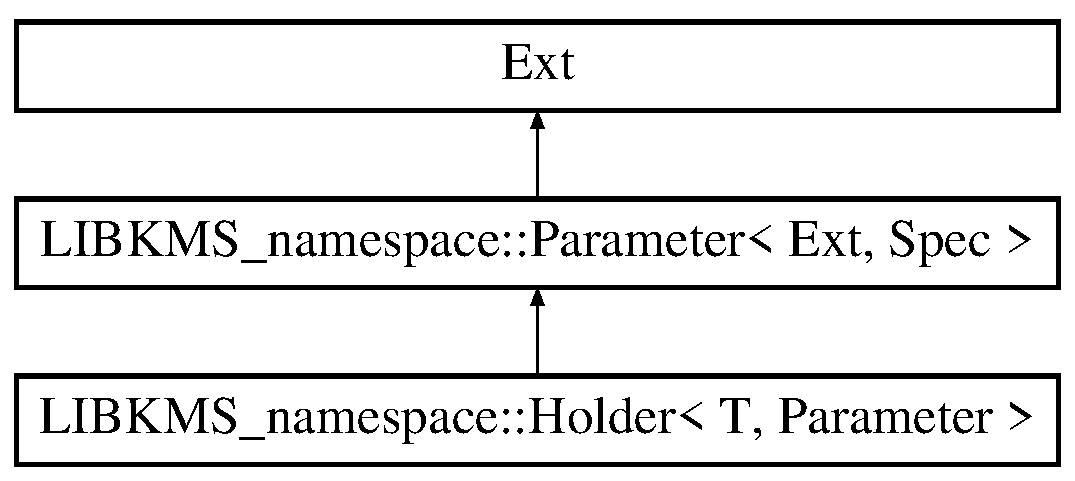
\includegraphics[height=3.000000cm]{classLIBKMS__namespace_1_1Holder}
\end{center}
\end{figure}
\subsection*{Открытые члены}
\begin{DoxyCompactItemize}
\item 
\hyperlink{classLIBKMS__namespace_1_1Holder_aaf783d1d73c737a24a8c3d7908e5fb38}{Holder} ()
\item 
\hyperlink{classLIBKMS__namespace_1_1Holder_a072572ebd10dfab076746505589e1524}{Holder} (const T \&data)
\item 
\hyperlink{classLIBKMS__namespace_1_1Holder_ae083c92525080cda7e07f0613219bf50}{operator T} () const 
\begin{DoxyCompactList}\small\item\em Вернуть сохраненное значение \end{DoxyCompactList}\item 
\hyperlink{classLIBKMS__namespace_1_1Holder}{holder\-\_\-t} \& \hyperlink{classLIBKMS__namespace_1_1Holder_a731cef724723c5b2c7b8e54eb7adf162}{operator=} (const T val)
\begin{DoxyCompactList}\small\item\em Записать новое значение \end{DoxyCompactList}\item 
void \hyperlink{classLIBKMS__namespace_1_1Holder_a8ea748f417acec33c92a0879168977f1}{set\-\_\-value} (const T val)
\item 
T \hyperlink{classLIBKMS__namespace_1_1Holder_ad2e6c1867dc854db40a960623f79965d}{get\-\_\-value} () const 
\item 
parameter\-\_\-ptr \hyperlink{classLIBKMS__namespace_1_1Holder_aff9b8117c9662d48700365dac518a973}{clone} ()
\item 
std\-::string \hyperlink{classLIBKMS__namespace_1_1Holder_a4a52e97abc2329b4de3188c8ee2437b7}{to\-\_\-string} () const 
\begin{DoxyCompactList}\small\item\em Вернуть представление данных в виде строки \end{DoxyCompactList}\item 
bool \hyperlink{classLIBKMS__namespace_1_1Holder_aadb0bc39195f64c5fdd1eebda4274175}{from\-\_\-string} (const std\-::string \&src)
\begin{DoxyCompactList}\small\item\em Записать значение из строки \end{DoxyCompactList}\item 
std\-::vector$<$ uint8\-\_\-t $>$ \hyperlink{classLIBKMS__namespace_1_1Holder_af3568f981e9862d1cdc85404c971f8fd}{to\-\_\-bytes} () const 
\begin{DoxyCompactList}\small\item\em Вернуть представление данных в виде вектора байтов \end{DoxyCompactList}\item 
bool \hyperlink{classLIBKMS__namespace_1_1Holder_a6c9274a0d762e36bd709baff85a4c8b2}{from\-\_\-bytes} (const uint8\-\_\-t $\ast$b, size\-\_\-t s)
\begin{DoxyCompactList}\small\item\em Записать значение из набора байтов \end{DoxyCompactList}\item 
bool \hyperlink{classLIBKMS__namespace_1_1Holder_a625053bf2acde4d625d3b25635478c9f}{is\-\_\-equal} (const \hyperlink{classLIBKMS__namespace_1_1Parameter}{parameter\-\_\-t} \&another) const 
\begin{DoxyCompactList}\small\item\em Проверка равны ли значения \end{DoxyCompactList}\item 
bool \hyperlink{classLIBKMS__namespace_1_1Holder_a25d1d8c9e5659fd2a2b0980031bf7166}{is\-\_\-set} () const 
\begin{DoxyCompactList}\small\item\em Является ли параметр установленным (для power-\/переменных) \end{DoxyCompactList}\item 
bool \hyperlink{classLIBKMS__namespace_1_1Holder_a9cb55778ffef92d63b954f1e07f56d58}{copy\-\_\-data} (\hyperlink{classLIBKMS__namespace_1_1Parameter}{parameter\-\_\-t} \&a)
\begin{DoxyCompactList}\small\item\em Скопировать значение из указанного контейнера \end{DoxyCompactList}\end{DoxyCompactItemize}
\subsection*{Защищенные данные}
\begin{DoxyCompactItemize}
\item 
T \hyperlink{classLIBKMS__namespace_1_1Holder_a7a9cd1db71653a8e0f93aa57276eedc0}{\-\_\-data}
\end{DoxyCompactItemize}
\subsection*{Дополнительные унаследованные члены}


\subsection{Подробное описание}
\subsubsection*{template$<$typename T, typename Parameter$>$class L\-I\-B\-K\-M\-S\-\_\-namespace\-::\-Holder$<$ T, Parameter $>$}

Класс-\/контейнер для стандартных типов 

\subsection{Конструктор(ы)}
\hypertarget{classLIBKMS__namespace_1_1Holder_aaf783d1d73c737a24a8c3d7908e5fb38}{\index{L\-I\-B\-K\-M\-S\-\_\-namespace\-::\-Holder@{L\-I\-B\-K\-M\-S\-\_\-namespace\-::\-Holder}!Holder@{Holder}}
\index{Holder@{Holder}!LIBKMS_namespace::Holder@{L\-I\-B\-K\-M\-S\-\_\-namespace\-::\-Holder}}
\subsubsection[{Holder}]{\setlength{\rightskip}{0pt plus 5cm}template$<$typename T , typename Parameter $>$ {\bf L\-I\-B\-K\-M\-S\-\_\-namespace\-::\-Holder}$<$ T, {\bf Parameter} $>$\-::{\bf Holder} (
\begin{DoxyParamCaption}
{}
\end{DoxyParamCaption}
)\hspace{0.3cm}{\ttfamily [inline]}}}\label{classLIBKMS__namespace_1_1Holder_aaf783d1d73c737a24a8c3d7908e5fb38}
\hypertarget{classLIBKMS__namespace_1_1Holder_a072572ebd10dfab076746505589e1524}{\index{L\-I\-B\-K\-M\-S\-\_\-namespace\-::\-Holder@{L\-I\-B\-K\-M\-S\-\_\-namespace\-::\-Holder}!Holder@{Holder}}
\index{Holder@{Holder}!LIBKMS_namespace::Holder@{L\-I\-B\-K\-M\-S\-\_\-namespace\-::\-Holder}}
\subsubsection[{Holder}]{\setlength{\rightskip}{0pt plus 5cm}template$<$typename T , typename Parameter $>$ {\bf L\-I\-B\-K\-M\-S\-\_\-namespace\-::\-Holder}$<$ T, {\bf Parameter} $>$\-::{\bf Holder} (
\begin{DoxyParamCaption}
\item[{const T \&}]{data}
\end{DoxyParamCaption}
)\hspace{0.3cm}{\ttfamily [inline]}}}\label{classLIBKMS__namespace_1_1Holder_a072572ebd10dfab076746505589e1524}


\subsection{Методы}
\hypertarget{classLIBKMS__namespace_1_1Holder_aff9b8117c9662d48700365dac518a973}{\index{L\-I\-B\-K\-M\-S\-\_\-namespace\-::\-Holder@{L\-I\-B\-K\-M\-S\-\_\-namespace\-::\-Holder}!clone@{clone}}
\index{clone@{clone}!LIBKMS_namespace::Holder@{L\-I\-B\-K\-M\-S\-\_\-namespace\-::\-Holder}}
\subsubsection[{clone}]{\setlength{\rightskip}{0pt plus 5cm}template$<$typename T , typename Parameter $>$ parameter\-\_\-ptr {\bf L\-I\-B\-K\-M\-S\-\_\-namespace\-::\-Holder}$<$ T, {\bf Parameter} $>$\-::clone (
\begin{DoxyParamCaption}
{}
\end{DoxyParamCaption}
)\hspace{0.3cm}{\ttfamily [inline]}, {\ttfamily [virtual]}}}\label{classLIBKMS__namespace_1_1Holder_aff9b8117c9662d48700365dac518a973}


Замещает \hyperlink{classLIBKMS__namespace_1_1Parameter_a2b360aeb7f850d4fccc58adc4a5b88b7}{L\-I\-B\-K\-M\-S\-\_\-namespace\-::\-Parameter$<$ Ext, Spec $>$}.

\hypertarget{classLIBKMS__namespace_1_1Holder_a9cb55778ffef92d63b954f1e07f56d58}{\index{L\-I\-B\-K\-M\-S\-\_\-namespace\-::\-Holder@{L\-I\-B\-K\-M\-S\-\_\-namespace\-::\-Holder}!copy\-\_\-data@{copy\-\_\-data}}
\index{copy\-\_\-data@{copy\-\_\-data}!LIBKMS_namespace::Holder@{L\-I\-B\-K\-M\-S\-\_\-namespace\-::\-Holder}}
\subsubsection[{copy\-\_\-data}]{\setlength{\rightskip}{0pt plus 5cm}template$<$typename T , typename Parameter $>$ bool {\bf L\-I\-B\-K\-M\-S\-\_\-namespace\-::\-Holder}$<$ T, {\bf Parameter} $>$\-::copy\-\_\-data (
\begin{DoxyParamCaption}
\item[{{\bf parameter\-\_\-t} \&}]{a}
\end{DoxyParamCaption}
)\hspace{0.3cm}{\ttfamily [inline]}}}\label{classLIBKMS__namespace_1_1Holder_a9cb55778ffef92d63b954f1e07f56d58}


Скопировать значение из указанного контейнера 

\hypertarget{classLIBKMS__namespace_1_1Holder_a6c9274a0d762e36bd709baff85a4c8b2}{\index{L\-I\-B\-K\-M\-S\-\_\-namespace\-::\-Holder@{L\-I\-B\-K\-M\-S\-\_\-namespace\-::\-Holder}!from\-\_\-bytes@{from\-\_\-bytes}}
\index{from\-\_\-bytes@{from\-\_\-bytes}!LIBKMS_namespace::Holder@{L\-I\-B\-K\-M\-S\-\_\-namespace\-::\-Holder}}
\subsubsection[{from\-\_\-bytes}]{\setlength{\rightskip}{0pt plus 5cm}template$<$typename T , typename Parameter $>$ bool {\bf L\-I\-B\-K\-M\-S\-\_\-namespace\-::\-Holder}$<$ T, {\bf Parameter} $>$\-::from\-\_\-bytes (
\begin{DoxyParamCaption}
\item[{const uint8\-\_\-t $\ast$}]{b, }
\item[{size\-\_\-t}]{s}
\end{DoxyParamCaption}
)\hspace{0.3cm}{\ttfamily [inline]}, {\ttfamily [virtual]}}}\label{classLIBKMS__namespace_1_1Holder_a6c9274a0d762e36bd709baff85a4c8b2}


Записать значение из набора байтов 



Замещает \hyperlink{classLIBKMS__namespace_1_1Parameter_a33a7dac4680f0e39c9166771c65971ab}{L\-I\-B\-K\-M\-S\-\_\-namespace\-::\-Parameter$<$ Ext, Spec $>$}.

\hypertarget{classLIBKMS__namespace_1_1Holder_aadb0bc39195f64c5fdd1eebda4274175}{\index{L\-I\-B\-K\-M\-S\-\_\-namespace\-::\-Holder@{L\-I\-B\-K\-M\-S\-\_\-namespace\-::\-Holder}!from\-\_\-string@{from\-\_\-string}}
\index{from\-\_\-string@{from\-\_\-string}!LIBKMS_namespace::Holder@{L\-I\-B\-K\-M\-S\-\_\-namespace\-::\-Holder}}
\subsubsection[{from\-\_\-string}]{\setlength{\rightskip}{0pt plus 5cm}template$<$typename T , typename Parameter $>$ bool {\bf L\-I\-B\-K\-M\-S\-\_\-namespace\-::\-Holder}$<$ T, {\bf Parameter} $>$\-::from\-\_\-string (
\begin{DoxyParamCaption}
\item[{const std\-::string \&}]{src}
\end{DoxyParamCaption}
)\hspace{0.3cm}{\ttfamily [inline]}, {\ttfamily [virtual]}}}\label{classLIBKMS__namespace_1_1Holder_aadb0bc39195f64c5fdd1eebda4274175}


Записать значение из строки 



Замещает \hyperlink{classLIBKMS__namespace_1_1Parameter_a6da649d3045e979a488c336bf77b411b}{L\-I\-B\-K\-M\-S\-\_\-namespace\-::\-Parameter$<$ Ext, Spec $>$}.

\hypertarget{classLIBKMS__namespace_1_1Holder_ad2e6c1867dc854db40a960623f79965d}{\index{L\-I\-B\-K\-M\-S\-\_\-namespace\-::\-Holder@{L\-I\-B\-K\-M\-S\-\_\-namespace\-::\-Holder}!get\-\_\-value@{get\-\_\-value}}
\index{get\-\_\-value@{get\-\_\-value}!LIBKMS_namespace::Holder@{L\-I\-B\-K\-M\-S\-\_\-namespace\-::\-Holder}}
\subsubsection[{get\-\_\-value}]{\setlength{\rightskip}{0pt plus 5cm}template$<$typename T , typename Parameter $>$ T {\bf L\-I\-B\-K\-M\-S\-\_\-namespace\-::\-Holder}$<$ T, {\bf Parameter} $>$\-::get\-\_\-value (
\begin{DoxyParamCaption}
{}
\end{DoxyParamCaption}
) const\hspace{0.3cm}{\ttfamily [inline]}}}\label{classLIBKMS__namespace_1_1Holder_ad2e6c1867dc854db40a960623f79965d}
\hypertarget{classLIBKMS__namespace_1_1Holder_a625053bf2acde4d625d3b25635478c9f}{\index{L\-I\-B\-K\-M\-S\-\_\-namespace\-::\-Holder@{L\-I\-B\-K\-M\-S\-\_\-namespace\-::\-Holder}!is\-\_\-equal@{is\-\_\-equal}}
\index{is\-\_\-equal@{is\-\_\-equal}!LIBKMS_namespace::Holder@{L\-I\-B\-K\-M\-S\-\_\-namespace\-::\-Holder}}
\subsubsection[{is\-\_\-equal}]{\setlength{\rightskip}{0pt plus 5cm}template$<$typename T , typename Parameter $>$ bool {\bf L\-I\-B\-K\-M\-S\-\_\-namespace\-::\-Holder}$<$ T, {\bf Parameter} $>$\-::is\-\_\-equal (
\begin{DoxyParamCaption}
\item[{const {\bf parameter\-\_\-t} \&}]{another}
\end{DoxyParamCaption}
) const\hspace{0.3cm}{\ttfamily [inline]}}}\label{classLIBKMS__namespace_1_1Holder_a625053bf2acde4d625d3b25635478c9f}


Проверка равны ли значения 

\hypertarget{classLIBKMS__namespace_1_1Holder_a25d1d8c9e5659fd2a2b0980031bf7166}{\index{L\-I\-B\-K\-M\-S\-\_\-namespace\-::\-Holder@{L\-I\-B\-K\-M\-S\-\_\-namespace\-::\-Holder}!is\-\_\-set@{is\-\_\-set}}
\index{is\-\_\-set@{is\-\_\-set}!LIBKMS_namespace::Holder@{L\-I\-B\-K\-M\-S\-\_\-namespace\-::\-Holder}}
\subsubsection[{is\-\_\-set}]{\setlength{\rightskip}{0pt plus 5cm}template$<$typename T , typename Parameter $>$ bool {\bf L\-I\-B\-K\-M\-S\-\_\-namespace\-::\-Holder}$<$ T, {\bf Parameter} $>$\-::is\-\_\-set (
\begin{DoxyParamCaption}
{}
\end{DoxyParamCaption}
) const\hspace{0.3cm}{\ttfamily [inline]}, {\ttfamily [virtual]}}}\label{classLIBKMS__namespace_1_1Holder_a25d1d8c9e5659fd2a2b0980031bf7166}


Является ли параметр установленным (для power-\/переменных) 



Замещает \hyperlink{classLIBKMS__namespace_1_1Parameter_ac46dd4bb2e060a4e5f522b625cb44b11}{L\-I\-B\-K\-M\-S\-\_\-namespace\-::\-Parameter$<$ Ext, Spec $>$}.

\hypertarget{classLIBKMS__namespace_1_1Holder_ae083c92525080cda7e07f0613219bf50}{\index{L\-I\-B\-K\-M\-S\-\_\-namespace\-::\-Holder@{L\-I\-B\-K\-M\-S\-\_\-namespace\-::\-Holder}!operator T@{operator T}}
\index{operator T@{operator T}!LIBKMS_namespace::Holder@{L\-I\-B\-K\-M\-S\-\_\-namespace\-::\-Holder}}
\subsubsection[{operator T}]{\setlength{\rightskip}{0pt plus 5cm}template$<$typename T , typename Parameter $>$ {\bf L\-I\-B\-K\-M\-S\-\_\-namespace\-::\-Holder}$<$ T, {\bf Parameter} $>$\-::operator T (
\begin{DoxyParamCaption}
{}
\end{DoxyParamCaption}
) const\hspace{0.3cm}{\ttfamily [inline]}}}\label{classLIBKMS__namespace_1_1Holder_ae083c92525080cda7e07f0613219bf50}


Вернуть сохраненное значение 

\hypertarget{classLIBKMS__namespace_1_1Holder_a731cef724723c5b2c7b8e54eb7adf162}{\index{L\-I\-B\-K\-M\-S\-\_\-namespace\-::\-Holder@{L\-I\-B\-K\-M\-S\-\_\-namespace\-::\-Holder}!operator=@{operator=}}
\index{operator=@{operator=}!LIBKMS_namespace::Holder@{L\-I\-B\-K\-M\-S\-\_\-namespace\-::\-Holder}}
\subsubsection[{operator=}]{\setlength{\rightskip}{0pt plus 5cm}template$<$typename T , typename Parameter $>$ {\bf holder\-\_\-t}\& {\bf L\-I\-B\-K\-M\-S\-\_\-namespace\-::\-Holder}$<$ T, {\bf Parameter} $>$\-::operator= (
\begin{DoxyParamCaption}
\item[{const T}]{val}
\end{DoxyParamCaption}
)\hspace{0.3cm}{\ttfamily [inline]}}}\label{classLIBKMS__namespace_1_1Holder_a731cef724723c5b2c7b8e54eb7adf162}


Записать новое значение 

\hypertarget{classLIBKMS__namespace_1_1Holder_a8ea748f417acec33c92a0879168977f1}{\index{L\-I\-B\-K\-M\-S\-\_\-namespace\-::\-Holder@{L\-I\-B\-K\-M\-S\-\_\-namespace\-::\-Holder}!set\-\_\-value@{set\-\_\-value}}
\index{set\-\_\-value@{set\-\_\-value}!LIBKMS_namespace::Holder@{L\-I\-B\-K\-M\-S\-\_\-namespace\-::\-Holder}}
\subsubsection[{set\-\_\-value}]{\setlength{\rightskip}{0pt plus 5cm}template$<$typename T , typename Parameter $>$ void {\bf L\-I\-B\-K\-M\-S\-\_\-namespace\-::\-Holder}$<$ T, {\bf Parameter} $>$\-::set\-\_\-value (
\begin{DoxyParamCaption}
\item[{const T}]{val}
\end{DoxyParamCaption}
)\hspace{0.3cm}{\ttfamily [inline]}}}\label{classLIBKMS__namespace_1_1Holder_a8ea748f417acec33c92a0879168977f1}
\hypertarget{classLIBKMS__namespace_1_1Holder_af3568f981e9862d1cdc85404c971f8fd}{\index{L\-I\-B\-K\-M\-S\-\_\-namespace\-::\-Holder@{L\-I\-B\-K\-M\-S\-\_\-namespace\-::\-Holder}!to\-\_\-bytes@{to\-\_\-bytes}}
\index{to\-\_\-bytes@{to\-\_\-bytes}!LIBKMS_namespace::Holder@{L\-I\-B\-K\-M\-S\-\_\-namespace\-::\-Holder}}
\subsubsection[{to\-\_\-bytes}]{\setlength{\rightskip}{0pt plus 5cm}template$<$typename T , typename Parameter $>$ std\-::vector$<$ uint8\-\_\-t $>$ {\bf L\-I\-B\-K\-M\-S\-\_\-namespace\-::\-Holder}$<$ T, {\bf Parameter} $>$\-::to\-\_\-bytes (
\begin{DoxyParamCaption}
{}
\end{DoxyParamCaption}
) const\hspace{0.3cm}{\ttfamily [inline]}, {\ttfamily [virtual]}}}\label{classLIBKMS__namespace_1_1Holder_af3568f981e9862d1cdc85404c971f8fd}


Вернуть представление данных в виде вектора байтов 



Замещает \hyperlink{classLIBKMS__namespace_1_1Parameter_a6ebf9bc6aaa62d78f786bc6368a2c65a}{L\-I\-B\-K\-M\-S\-\_\-namespace\-::\-Parameter$<$ Ext, Spec $>$}.

\hypertarget{classLIBKMS__namespace_1_1Holder_a4a52e97abc2329b4de3188c8ee2437b7}{\index{L\-I\-B\-K\-M\-S\-\_\-namespace\-::\-Holder@{L\-I\-B\-K\-M\-S\-\_\-namespace\-::\-Holder}!to\-\_\-string@{to\-\_\-string}}
\index{to\-\_\-string@{to\-\_\-string}!LIBKMS_namespace::Holder@{L\-I\-B\-K\-M\-S\-\_\-namespace\-::\-Holder}}
\subsubsection[{to\-\_\-string}]{\setlength{\rightskip}{0pt plus 5cm}template$<$typename T , typename Parameter $>$ std\-::string {\bf L\-I\-B\-K\-M\-S\-\_\-namespace\-::\-Holder}$<$ T, {\bf Parameter} $>$\-::to\-\_\-string (
\begin{DoxyParamCaption}
{}
\end{DoxyParamCaption}
) const\hspace{0.3cm}{\ttfamily [inline]}, {\ttfamily [virtual]}}}\label{classLIBKMS__namespace_1_1Holder_a4a52e97abc2329b4de3188c8ee2437b7}


Вернуть представление данных в виде строки 



Замещает \hyperlink{classLIBKMS__namespace_1_1Parameter_ad934454e1569e546f6f347bb03ce705f}{L\-I\-B\-K\-M\-S\-\_\-namespace\-::\-Parameter$<$ Ext, Spec $>$}.



\subsection{Данные класса}
\hypertarget{classLIBKMS__namespace_1_1Holder_a7a9cd1db71653a8e0f93aa57276eedc0}{\index{L\-I\-B\-K\-M\-S\-\_\-namespace\-::\-Holder@{L\-I\-B\-K\-M\-S\-\_\-namespace\-::\-Holder}!\-\_\-data@{\-\_\-data}}
\index{\-\_\-data@{\-\_\-data}!LIBKMS_namespace::Holder@{L\-I\-B\-K\-M\-S\-\_\-namespace\-::\-Holder}}
\subsubsection[{\-\_\-data}]{\setlength{\rightskip}{0pt plus 5cm}template$<$typename T , typename Parameter $>$ T {\bf L\-I\-B\-K\-M\-S\-\_\-namespace\-::\-Holder}$<$ T, {\bf Parameter} $>$\-::\-\_\-data\hspace{0.3cm}{\ttfamily [protected]}}}\label{classLIBKMS__namespace_1_1Holder_a7a9cd1db71653a8e0f93aa57276eedc0}


Объявления и описания членов класса находятся в файле\-:\begin{DoxyCompactItemize}
\item 
\hyperlink{holder_8hpp}{holder.\-hpp}\end{DoxyCompactItemize}

\hypertarget{classLIBKMS__namespace_1_1exception_1_1invalid__type}{\section{Класс L\-I\-B\-K\-M\-S\-\_\-namespace\-:\-:exception\-:\-:invalid\-\_\-type}
\label{classLIBKMS__namespace_1_1exception_1_1invalid__type}\index{L\-I\-B\-K\-M\-S\-\_\-namespace\-::exception\-::invalid\-\_\-type@{L\-I\-B\-K\-M\-S\-\_\-namespace\-::exception\-::invalid\-\_\-type}}
}


{\ttfamily \#include $<$holder.\-hpp$>$}

Граф наследования\-:L\-I\-B\-K\-M\-S\-\_\-namespace\-:\-:exception\-:\-:invalid\-\_\-type\-:\begin{figure}[H]
\begin{center}
\leavevmode
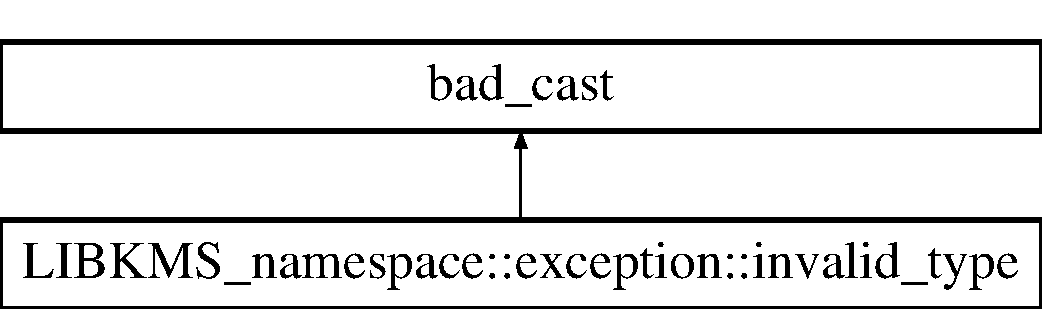
\includegraphics[height=2.000000cm]{classLIBKMS__namespace_1_1exception_1_1invalid__type}
\end{center}
\end{figure}
\subsection*{Открытые члены}
\begin{DoxyCompactItemize}
\item 
\hyperlink{classLIBKMS__namespace_1_1exception_1_1invalid__type_aa01d2777535f5d5765c852b1a64489d7}{invalid\-\_\-type} (const std\-::string \&name)
\item 
std\-::string \hyperlink{classLIBKMS__namespace_1_1exception_1_1invalid__type_ab3b73d66e93392987197718e4b7c7b6f}{get\-\_\-name} ()
\end{DoxyCompactItemize}


\subsection{Конструктор(ы)}
\hypertarget{classLIBKMS__namespace_1_1exception_1_1invalid__type_aa01d2777535f5d5765c852b1a64489d7}{\index{L\-I\-B\-K\-M\-S\-\_\-namespace\-::exception\-::invalid\-\_\-type@{L\-I\-B\-K\-M\-S\-\_\-namespace\-::exception\-::invalid\-\_\-type}!invalid\-\_\-type@{invalid\-\_\-type}}
\index{invalid\-\_\-type@{invalid\-\_\-type}!LIBKMS_namespace::exception::invalid_type@{L\-I\-B\-K\-M\-S\-\_\-namespace\-::exception\-::invalid\-\_\-type}}
\subsubsection[{invalid\-\_\-type}]{\setlength{\rightskip}{0pt plus 5cm}L\-I\-B\-K\-M\-S\-\_\-namespace\-::exception\-::invalid\-\_\-type\-::invalid\-\_\-type (
\begin{DoxyParamCaption}
\item[{const std\-::string \&}]{name}
\end{DoxyParamCaption}
)\hspace{0.3cm}{\ttfamily [inline]}}}\label{classLIBKMS__namespace_1_1exception_1_1invalid__type_aa01d2777535f5d5765c852b1a64489d7}


\subsection{Методы}
\hypertarget{classLIBKMS__namespace_1_1exception_1_1invalid__type_ab3b73d66e93392987197718e4b7c7b6f}{\index{L\-I\-B\-K\-M\-S\-\_\-namespace\-::exception\-::invalid\-\_\-type@{L\-I\-B\-K\-M\-S\-\_\-namespace\-::exception\-::invalid\-\_\-type}!get\-\_\-name@{get\-\_\-name}}
\index{get\-\_\-name@{get\-\_\-name}!LIBKMS_namespace::exception::invalid_type@{L\-I\-B\-K\-M\-S\-\_\-namespace\-::exception\-::invalid\-\_\-type}}
\subsubsection[{get\-\_\-name}]{\setlength{\rightskip}{0pt plus 5cm}std\-::string L\-I\-B\-K\-M\-S\-\_\-namespace\-::exception\-::invalid\-\_\-type\-::get\-\_\-name (
\begin{DoxyParamCaption}
{}
\end{DoxyParamCaption}
)\hspace{0.3cm}{\ttfamily [inline]}}}\label{classLIBKMS__namespace_1_1exception_1_1invalid__type_ab3b73d66e93392987197718e4b7c7b6f}


Объявления и описания членов класса находятся в файле\-:\begin{DoxyCompactItemize}
\item 
\hyperlink{holder_8hpp}{holder.\-hpp}\end{DoxyCompactItemize}

\hypertarget{classLIBKMS__namespace_1_1exception_1_1invalid__var__name}{\section{Класс L\-I\-B\-K\-M\-S\-\_\-namespace\-:\-:exception\-:\-:invalid\-\_\-var\-\_\-name}
\label{classLIBKMS__namespace_1_1exception_1_1invalid__var__name}\index{L\-I\-B\-K\-M\-S\-\_\-namespace\-::exception\-::invalid\-\_\-var\-\_\-name@{L\-I\-B\-K\-M\-S\-\_\-namespace\-::exception\-::invalid\-\_\-var\-\_\-name}}
}


{\ttfamily \#include $<$holder.\-hpp$>$}

Граф наследования\-:L\-I\-B\-K\-M\-S\-\_\-namespace\-:\-:exception\-:\-:invalid\-\_\-var\-\_\-name\-:\begin{figure}[H]
\begin{center}
\leavevmode
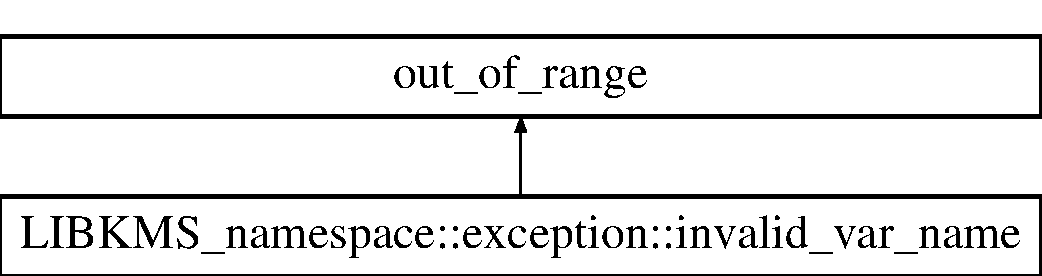
\includegraphics[height=2.000000cm]{classLIBKMS__namespace_1_1exception_1_1invalid__var__name}
\end{center}
\end{figure}
\subsection*{Открытые члены}
\begin{DoxyCompactItemize}
\item 
\hyperlink{classLIBKMS__namespace_1_1exception_1_1invalid__var__name_a567be995b9cbc2548099512f7a0288a1}{invalid\-\_\-var\-\_\-name} (const std\-::string \&name)
\item 
std\-::string \hyperlink{classLIBKMS__namespace_1_1exception_1_1invalid__var__name_aed697e974d9b0dd20faa0ff5d72a5ee3}{get\-\_\-name} ()
\end{DoxyCompactItemize}


\subsection{Конструктор(ы)}
\hypertarget{classLIBKMS__namespace_1_1exception_1_1invalid__var__name_a567be995b9cbc2548099512f7a0288a1}{\index{L\-I\-B\-K\-M\-S\-\_\-namespace\-::exception\-::invalid\-\_\-var\-\_\-name@{L\-I\-B\-K\-M\-S\-\_\-namespace\-::exception\-::invalid\-\_\-var\-\_\-name}!invalid\-\_\-var\-\_\-name@{invalid\-\_\-var\-\_\-name}}
\index{invalid\-\_\-var\-\_\-name@{invalid\-\_\-var\-\_\-name}!LIBKMS_namespace::exception::invalid_var_name@{L\-I\-B\-K\-M\-S\-\_\-namespace\-::exception\-::invalid\-\_\-var\-\_\-name}}
\subsubsection[{invalid\-\_\-var\-\_\-name}]{\setlength{\rightskip}{0pt plus 5cm}L\-I\-B\-K\-M\-S\-\_\-namespace\-::exception\-::invalid\-\_\-var\-\_\-name\-::invalid\-\_\-var\-\_\-name (
\begin{DoxyParamCaption}
\item[{const std\-::string \&}]{name}
\end{DoxyParamCaption}
)\hspace{0.3cm}{\ttfamily [inline]}}}\label{classLIBKMS__namespace_1_1exception_1_1invalid__var__name_a567be995b9cbc2548099512f7a0288a1}


\subsection{Методы}
\hypertarget{classLIBKMS__namespace_1_1exception_1_1invalid__var__name_aed697e974d9b0dd20faa0ff5d72a5ee3}{\index{L\-I\-B\-K\-M\-S\-\_\-namespace\-::exception\-::invalid\-\_\-var\-\_\-name@{L\-I\-B\-K\-M\-S\-\_\-namespace\-::exception\-::invalid\-\_\-var\-\_\-name}!get\-\_\-name@{get\-\_\-name}}
\index{get\-\_\-name@{get\-\_\-name}!LIBKMS_namespace::exception::invalid_var_name@{L\-I\-B\-K\-M\-S\-\_\-namespace\-::exception\-::invalid\-\_\-var\-\_\-name}}
\subsubsection[{get\-\_\-name}]{\setlength{\rightskip}{0pt plus 5cm}std\-::string L\-I\-B\-K\-M\-S\-\_\-namespace\-::exception\-::invalid\-\_\-var\-\_\-name\-::get\-\_\-name (
\begin{DoxyParamCaption}
{}
\end{DoxyParamCaption}
)\hspace{0.3cm}{\ttfamily [inline]}}}\label{classLIBKMS__namespace_1_1exception_1_1invalid__var__name_aed697e974d9b0dd20faa0ff5d72a5ee3}


Объявления и описания членов класса находятся в файле\-:\begin{DoxyCompactItemize}
\item 
\hyperlink{holder_8hpp}{holder.\-hpp}\end{DoxyCompactItemize}

\hypertarget{structLIBKMS__namespace_1_1obj__as_3_01Holder_3_01T_00_01P_01_4_00_01P_01_4}{\section{Шаблон структуры L\-I\-B\-K\-M\-S\-\_\-namespace\-:\-:obj\-\_\-as$<$ Holder$<$ T, P $>$, P $>$}
\label{structLIBKMS__namespace_1_1obj__as_3_01Holder_3_01T_00_01P_01_4_00_01P_01_4}\index{L\-I\-B\-K\-M\-S\-\_\-namespace\-::obj\-\_\-as$<$ Holder$<$ T, P $>$, P $>$@{L\-I\-B\-K\-M\-S\-\_\-namespace\-::obj\-\_\-as$<$ Holder$<$ T, P $>$, P $>$}}
}


Специализация для преобразования parameter в Holder$<$ T $>$  




{\ttfamily \#include $<$holder.\-hpp$>$}

\subsection*{Открытые типы}
\begin{DoxyCompactItemize}
\item 
typedef \hyperlink{classLIBKMS__namespace_1_1Holder}{Holder}$<$ T, P $>$ \hyperlink{structLIBKMS__namespace_1_1obj__as_3_01Holder_3_01T_00_01P_01_4_00_01P_01_4_aa25f14fd65890cd92986509117d1dd7b}{holder\-\_\-t}
\end{DoxyCompactItemize}
\subsection*{Открытые статические члены}
\begin{DoxyCompactItemize}
\item 
static \hyperlink{structLIBKMS__namespace_1_1obj__as_3_01Holder_3_01T_00_01P_01_4_00_01P_01_4_aa25f14fd65890cd92986509117d1dd7b}{holder\-\_\-t} \& \hyperlink{structLIBKMS__namespace_1_1obj__as_3_01Holder_3_01T_00_01P_01_4_00_01P_01_4_a68c5ed911c1996920c3f40fb2cfe43d7}{as} (P \&obj)
\item 
static const \hyperlink{structLIBKMS__namespace_1_1obj__as_3_01Holder_3_01T_00_01P_01_4_00_01P_01_4_aa25f14fd65890cd92986509117d1dd7b}{holder\-\_\-t} \& \hyperlink{structLIBKMS__namespace_1_1obj__as_3_01Holder_3_01T_00_01P_01_4_00_01P_01_4_a05795aa17b8a30e1b7113fb7672cf278}{c\-\_\-as} (const P \&obj)
\end{DoxyCompactItemize}


\subsection{Подробное описание}
\subsubsection*{template$<$typename T, typename P$>$struct L\-I\-B\-K\-M\-S\-\_\-namespace\-::obj\-\_\-as$<$ Holder$<$ T, P $>$, P $>$}

Специализация для преобразования parameter в Holder$<$ T $>$ 

\subsection{Определения типов}
\hypertarget{structLIBKMS__namespace_1_1obj__as_3_01Holder_3_01T_00_01P_01_4_00_01P_01_4_aa25f14fd65890cd92986509117d1dd7b}{\index{L\-I\-B\-K\-M\-S\-\_\-namespace\-::obj\-\_\-as$<$ Holder$<$ T, P $>$, P $>$@{L\-I\-B\-K\-M\-S\-\_\-namespace\-::obj\-\_\-as$<$ Holder$<$ T, P $>$, P $>$}!holder\-\_\-t@{holder\-\_\-t}}
\index{holder\-\_\-t@{holder\-\_\-t}!LIBKMS_namespace::obj_as< Holder< T, P >, P >@{L\-I\-B\-K\-M\-S\-\_\-namespace\-::obj\-\_\-as$<$ Holder$<$ T, P $>$, P $>$}}
\subsubsection[{holder\-\_\-t}]{\setlength{\rightskip}{0pt plus 5cm}template$<$typename T , typename P $>$ typedef {\bf Holder}$<$ T, P $>$ L\-I\-B\-K\-M\-S\-\_\-namespace\-::obj\-\_\-as$<$ {\bf Holder}$<$ T, P $>$, P $>$\-::{\bf holder\-\_\-t}}}\label{structLIBKMS__namespace_1_1obj__as_3_01Holder_3_01T_00_01P_01_4_00_01P_01_4_aa25f14fd65890cd92986509117d1dd7b}


\subsection{Методы}
\hypertarget{structLIBKMS__namespace_1_1obj__as_3_01Holder_3_01T_00_01P_01_4_00_01P_01_4_a68c5ed911c1996920c3f40fb2cfe43d7}{\index{L\-I\-B\-K\-M\-S\-\_\-namespace\-::obj\-\_\-as$<$ Holder$<$ T, P $>$, P $>$@{L\-I\-B\-K\-M\-S\-\_\-namespace\-::obj\-\_\-as$<$ Holder$<$ T, P $>$, P $>$}!as@{as}}
\index{as@{as}!LIBKMS_namespace::obj_as< Holder< T, P >, P >@{L\-I\-B\-K\-M\-S\-\_\-namespace\-::obj\-\_\-as$<$ Holder$<$ T, P $>$, P $>$}}
\subsubsection[{as}]{\setlength{\rightskip}{0pt plus 5cm}template$<$typename T , typename P $>$ static {\bf holder\-\_\-t}\& L\-I\-B\-K\-M\-S\-\_\-namespace\-::obj\-\_\-as$<$ {\bf Holder}$<$ T, P $>$, P $>$\-::as (
\begin{DoxyParamCaption}
\item[{P \&}]{obj}
\end{DoxyParamCaption}
)\hspace{0.3cm}{\ttfamily [inline]}, {\ttfamily [static]}}}\label{structLIBKMS__namespace_1_1obj__as_3_01Holder_3_01T_00_01P_01_4_00_01P_01_4_a68c5ed911c1996920c3f40fb2cfe43d7}
\hypertarget{structLIBKMS__namespace_1_1obj__as_3_01Holder_3_01T_00_01P_01_4_00_01P_01_4_a05795aa17b8a30e1b7113fb7672cf278}{\index{L\-I\-B\-K\-M\-S\-\_\-namespace\-::obj\-\_\-as$<$ Holder$<$ T, P $>$, P $>$@{L\-I\-B\-K\-M\-S\-\_\-namespace\-::obj\-\_\-as$<$ Holder$<$ T, P $>$, P $>$}!c\-\_\-as@{c\-\_\-as}}
\index{c\-\_\-as@{c\-\_\-as}!LIBKMS_namespace::obj_as< Holder< T, P >, P >@{L\-I\-B\-K\-M\-S\-\_\-namespace\-::obj\-\_\-as$<$ Holder$<$ T, P $>$, P $>$}}
\subsubsection[{c\-\_\-as}]{\setlength{\rightskip}{0pt plus 5cm}template$<$typename T , typename P $>$ static const {\bf holder\-\_\-t}\& L\-I\-B\-K\-M\-S\-\_\-namespace\-::obj\-\_\-as$<$ {\bf Holder}$<$ T, P $>$, P $>$\-::c\-\_\-as (
\begin{DoxyParamCaption}
\item[{const P \&}]{obj}
\end{DoxyParamCaption}
)\hspace{0.3cm}{\ttfamily [inline]}, {\ttfamily [static]}}}\label{structLIBKMS__namespace_1_1obj__as_3_01Holder_3_01T_00_01P_01_4_00_01P_01_4_a05795aa17b8a30e1b7113fb7672cf278}


Объявления и описания членов структуры находятся в файле\-:\begin{DoxyCompactItemize}
\item 
\hyperlink{holder_8hpp}{holder.\-hpp}\end{DoxyCompactItemize}

\hypertarget{classLIBKMS__namespace_1_1Parameter}{\section{Шаблон класса L\-I\-B\-K\-M\-S\-\_\-namespace\-:\-:Parameter$<$ Ext, Spec $>$}
\label{classLIBKMS__namespace_1_1Parameter}\index{L\-I\-B\-K\-M\-S\-\_\-namespace\-::\-Parameter$<$ Ext, Spec $>$@{L\-I\-B\-K\-M\-S\-\_\-namespace\-::\-Parameter$<$ Ext, Spec $>$}}
}


Класс, от которого должны наследоваться все классы параметров  




{\ttfamily \#include $<$param.\-hpp$>$}

Граф наследования\-:L\-I\-B\-K\-M\-S\-\_\-namespace\-:\-:Parameter$<$ Ext, Spec $>$\-:\begin{figure}[H]
\begin{center}
\leavevmode
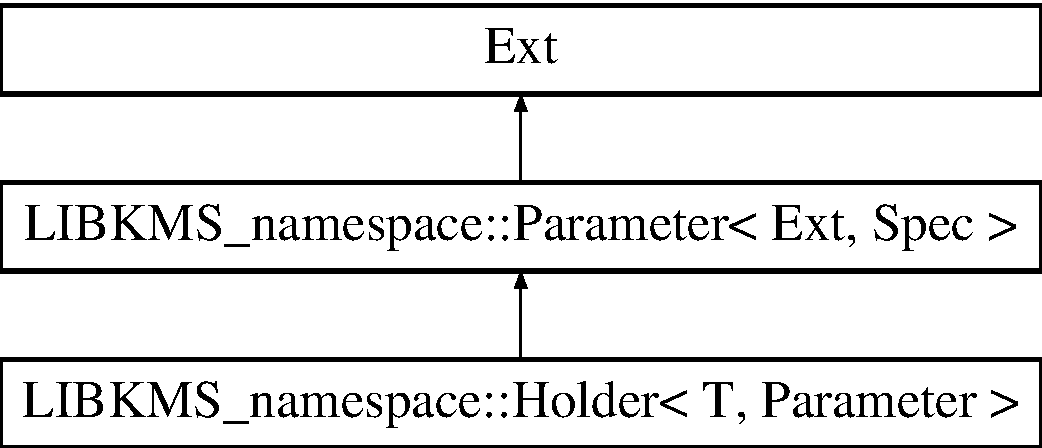
\includegraphics[height=3.000000cm]{classLIBKMS__namespace_1_1Parameter}
\end{center}
\end{figure}
\subsection*{Открытые типы}
\begin{DoxyCompactItemize}
\item 
typedef \hyperlink{classLIBKMS__namespace_1_1Parameter}{Parameter}$<$ Ext, Spec $>$ \hyperlink{classLIBKMS__namespace_1_1Parameter_af353e23edea754f9a2d1c936cd5c8eab}{parameter\-\_\-t}
\item 
typedef Spec$<$ \hyperlink{classLIBKMS__namespace_1_1Parameter_af353e23edea754f9a2d1c936cd5c8eab}{parameter\-\_\-t} $>$\-::ptr \hyperlink{classLIBKMS__namespace_1_1Parameter_a28516bcd5bad5857b2d1c676e4176f51}{ptr\-\_\-t}
\end{DoxyCompactItemize}
\subsection*{Открытые члены}
\begin{DoxyCompactItemize}
\item 
\hyperlink{classLIBKMS__namespace_1_1Parameter_ac767db81c6aa9e552089be5958bfc81f}{Parameter} ()
\item 
\hyperlink{classLIBKMS__namespace_1_1Parameter_a3c0c7c0222fbe9d6d38e002e706cf1b7}{Parameter} (const std\-::string type\-\_\-name)
\item 
virtual \hyperlink{classLIBKMS__namespace_1_1Parameter_a644c4a3c66079510847da3377e5f1594}{$\sim$\-Parameter} ()
\item 
virtual \hyperlink{classLIBKMS__namespace_1_1Parameter_a28516bcd5bad5857b2d1c676e4176f51}{ptr\-\_\-t} \hyperlink{classLIBKMS__namespace_1_1Parameter_a2b360aeb7f850d4fccc58adc4a5b88b7}{clone} ()=0
\item 
virtual std\-::string \hyperlink{classLIBKMS__namespace_1_1Parameter_ad934454e1569e546f6f347bb03ce705f}{to\-\_\-string} () const =0
\begin{DoxyCompactList}\small\item\em Вернуть представление данных в виде строки \end{DoxyCompactList}\item 
virtual bool \hyperlink{classLIBKMS__namespace_1_1Parameter_a6da649d3045e979a488c336bf77b411b}{from\-\_\-string} (const std\-::string \&)=0
\begin{DoxyCompactList}\small\item\em Записать значение из строки \end{DoxyCompactList}\item 
virtual std\-::vector$<$ uint8\-\_\-t $>$ \hyperlink{classLIBKMS__namespace_1_1Parameter_a6ebf9bc6aaa62d78f786bc6368a2c65a}{to\-\_\-bytes} () const =0
\begin{DoxyCompactList}\small\item\em Вернуть представление данных в виде вектора байтов \end{DoxyCompactList}\item 
virtual bool \hyperlink{classLIBKMS__namespace_1_1Parameter_a33a7dac4680f0e39c9166771c65971ab}{from\-\_\-bytes} (const uint8\-\_\-t $\ast$, size\-\_\-t)=0
\begin{DoxyCompactList}\small\item\em Записать значение из набора байтов \end{DoxyCompactList}\item 
virtual bool \hyperlink{classLIBKMS__namespace_1_1Parameter_a2f582483707d9229a5a2bde88d860fff}{is\-\_\-equal} (const \hyperlink{classLIBKMS__namespace_1_1Parameter_af353e23edea754f9a2d1c936cd5c8eab}{parameter\-\_\-t} \&another) const =0
\begin{DoxyCompactList}\small\item\em Сравнить значения \end{DoxyCompactList}\item 
virtual bool \hyperlink{classLIBKMS__namespace_1_1Parameter_ac46dd4bb2e060a4e5f522b625cb44b11}{is\-\_\-set} () const =0
\begin{DoxyCompactList}\small\item\em Является ли параметр установленным (для power-\/переменных) \end{DoxyCompactList}\item 
std\-::string \hyperlink{classLIBKMS__namespace_1_1Parameter_a7d03af2df98ad4053433f84288f0e786}{get\-\_\-type} () const 
\begin{DoxyCompactList}\small\item\em Вернуть имя типа \end{DoxyCompactList}\item 
virtual bool \hyperlink{classLIBKMS__namespace_1_1Parameter_a506fa08096a6595f04341b90912f35a0}{copy\-\_\-data} (\hyperlink{classLIBKMS__namespace_1_1Parameter_af353e23edea754f9a2d1c936cd5c8eab}{parameter\-\_\-t} \&)=0
\item 
{\footnotesize template$<$typename T $>$ }\\\hyperlink{structLIBKMS__namespace_1_1types_1_1get__return__type}{types\-::get\-\_\-return\-\_\-type}$<$ T, \\*
\hyperlink{classLIBKMS__namespace_1_1Parameter_af353e23edea754f9a2d1c936cd5c8eab}{parameter\-\_\-t} $>$\-::return\-\_\-t \hyperlink{classLIBKMS__namespace_1_1Parameter_ae6f38891ce947733703c3de5aafce38c}{as} ()
\item 
{\footnotesize template$<$typename T $>$ }\\const \hyperlink{structLIBKMS__namespace_1_1types_1_1get__return__type}{types\-::get\-\_\-return\-\_\-type}\\*
$<$ T, \hyperlink{classLIBKMS__namespace_1_1Parameter_af353e23edea754f9a2d1c936cd5c8eab}{parameter\-\_\-t} $>$\-::return\-\_\-t \hyperlink{classLIBKMS__namespace_1_1Parameter_a75fd27c3385b7474e99d501e4118702a}{c\-\_\-as} () const 
\item 
void \hyperlink{classLIBKMS__namespace_1_1Parameter_a688e383ed05a421a5b74f3d9a8780fad}{set\-\_\-desc} (const std\-::string \&d)
\begin{DoxyCompactList}\small\item\em Устанавливает описание переменной \end{DoxyCompactList}\item 
const std\-::string \& \hyperlink{classLIBKMS__namespace_1_1Parameter_a5696d8f34e854cae392e96ecca20e6c0}{get\-\_\-desc} () const 
\begin{DoxyCompactList}\small\item\em Возвращает описание переменной \end{DoxyCompactList}\item 
bool \hyperlink{classLIBKMS__namespace_1_1Parameter_a1bc31e7df8a2b5c68bec3ca3300af114}{is\-\_\-locked} () const 
\begin{DoxyCompactList}\small\item\em Возвращает признак блокировки \end{DoxyCompactList}\item 
void \hyperlink{classLIBKMS__namespace_1_1Parameter_aea87ceb7edf34c23aa5ec9240cd90673}{set\-\_\-lock} (bool \hyperlink{classLIBKMS__namespace_1_1Parameter_a1bc31e7df8a2b5c68bec3ca3300af114}{is\-\_\-locked})
\begin{DoxyCompactList}\small\item\em Блокирует переменную \end{DoxyCompactList}\end{DoxyCompactItemize}
\subsection*{Открытые статические члены}
\begin{DoxyCompactItemize}
\item 
static \hyperlink{classLIBKMS__namespace_1_1Parameter_a28516bcd5bad5857b2d1c676e4176f51}{ptr\-\_\-t} \hyperlink{classLIBKMS__namespace_1_1Parameter_a3978d2027190f56451d37703d7e317a2}{null\-\_\-ptr} ()
\end{DoxyCompactItemize}


\subsection{Подробное описание}
\subsubsection*{template$<$class Ext, template$<$ typename U $>$ class Spec$>$class L\-I\-B\-K\-M\-S\-\_\-namespace\-::\-Parameter$<$ Ext, Spec $>$}

Класс, от которого должны наследоваться все классы параметров 

\subsection{Определения типов}
\hypertarget{classLIBKMS__namespace_1_1Parameter_af353e23edea754f9a2d1c936cd5c8eab}{\index{L\-I\-B\-K\-M\-S\-\_\-namespace\-::\-Parameter@{L\-I\-B\-K\-M\-S\-\_\-namespace\-::\-Parameter}!parameter\-\_\-t@{parameter\-\_\-t}}
\index{parameter\-\_\-t@{parameter\-\_\-t}!LIBKMS_namespace::Parameter@{L\-I\-B\-K\-M\-S\-\_\-namespace\-::\-Parameter}}
\subsubsection[{parameter\-\_\-t}]{\setlength{\rightskip}{0pt plus 5cm}template$<$class Ext, template$<$ typename U $>$ class Spec$>$ typedef {\bf Parameter}$<$ Ext, Spec $>$ {\bf L\-I\-B\-K\-M\-S\-\_\-namespace\-::\-Parameter}$<$ Ext, Spec $>$\-::{\bf parameter\-\_\-t}}}\label{classLIBKMS__namespace_1_1Parameter_af353e23edea754f9a2d1c936cd5c8eab}
\hypertarget{classLIBKMS__namespace_1_1Parameter_a28516bcd5bad5857b2d1c676e4176f51}{\index{L\-I\-B\-K\-M\-S\-\_\-namespace\-::\-Parameter@{L\-I\-B\-K\-M\-S\-\_\-namespace\-::\-Parameter}!ptr\-\_\-t@{ptr\-\_\-t}}
\index{ptr\-\_\-t@{ptr\-\_\-t}!LIBKMS_namespace::Parameter@{L\-I\-B\-K\-M\-S\-\_\-namespace\-::\-Parameter}}
\subsubsection[{ptr\-\_\-t}]{\setlength{\rightskip}{0pt plus 5cm}template$<$class Ext, template$<$ typename U $>$ class Spec$>$ typedef Spec$<$ {\bf parameter\-\_\-t} $>$\-::ptr {\bf L\-I\-B\-K\-M\-S\-\_\-namespace\-::\-Parameter}$<$ Ext, Spec $>$\-::{\bf ptr\-\_\-t}}}\label{classLIBKMS__namespace_1_1Parameter_a28516bcd5bad5857b2d1c676e4176f51}


\subsection{Конструктор(ы)}
\hypertarget{classLIBKMS__namespace_1_1Parameter_ac767db81c6aa9e552089be5958bfc81f}{\index{L\-I\-B\-K\-M\-S\-\_\-namespace\-::\-Parameter@{L\-I\-B\-K\-M\-S\-\_\-namespace\-::\-Parameter}!Parameter@{Parameter}}
\index{Parameter@{Parameter}!LIBKMS_namespace::Parameter@{L\-I\-B\-K\-M\-S\-\_\-namespace\-::\-Parameter}}
\subsubsection[{Parameter}]{\setlength{\rightskip}{0pt plus 5cm}template$<$class Ext, template$<$ typename U $>$ class Spec$>$ {\bf L\-I\-B\-K\-M\-S\-\_\-namespace\-::\-Parameter}$<$ Ext, Spec $>$\-::{\bf Parameter} (
\begin{DoxyParamCaption}
{}
\end{DoxyParamCaption}
)\hspace{0.3cm}{\ttfamily [inline]}}}\label{classLIBKMS__namespace_1_1Parameter_ac767db81c6aa9e552089be5958bfc81f}
\hypertarget{classLIBKMS__namespace_1_1Parameter_a3c0c7c0222fbe9d6d38e002e706cf1b7}{\index{L\-I\-B\-K\-M\-S\-\_\-namespace\-::\-Parameter@{L\-I\-B\-K\-M\-S\-\_\-namespace\-::\-Parameter}!Parameter@{Parameter}}
\index{Parameter@{Parameter}!LIBKMS_namespace::Parameter@{L\-I\-B\-K\-M\-S\-\_\-namespace\-::\-Parameter}}
\subsubsection[{Parameter}]{\setlength{\rightskip}{0pt plus 5cm}template$<$class Ext, template$<$ typename U $>$ class Spec$>$ {\bf L\-I\-B\-K\-M\-S\-\_\-namespace\-::\-Parameter}$<$ Ext, Spec $>$\-::{\bf Parameter} (
\begin{DoxyParamCaption}
\item[{const std\-::string}]{type\-\_\-name}
\end{DoxyParamCaption}
)\hspace{0.3cm}{\ttfamily [inline]}}}\label{classLIBKMS__namespace_1_1Parameter_a3c0c7c0222fbe9d6d38e002e706cf1b7}
\hypertarget{classLIBKMS__namespace_1_1Parameter_a644c4a3c66079510847da3377e5f1594}{\index{L\-I\-B\-K\-M\-S\-\_\-namespace\-::\-Parameter@{L\-I\-B\-K\-M\-S\-\_\-namespace\-::\-Parameter}!$\sim$\-Parameter@{$\sim$\-Parameter}}
\index{$\sim$\-Parameter@{$\sim$\-Parameter}!LIBKMS_namespace::Parameter@{L\-I\-B\-K\-M\-S\-\_\-namespace\-::\-Parameter}}
\subsubsection[{$\sim$\-Parameter}]{\setlength{\rightskip}{0pt plus 5cm}template$<$class Ext, template$<$ typename U $>$ class Spec$>$ virtual {\bf L\-I\-B\-K\-M\-S\-\_\-namespace\-::\-Parameter}$<$ Ext, Spec $>$\-::$\sim${\bf Parameter} (
\begin{DoxyParamCaption}
{}
\end{DoxyParamCaption}
)\hspace{0.3cm}{\ttfamily [inline]}, {\ttfamily [virtual]}}}\label{classLIBKMS__namespace_1_1Parameter_a644c4a3c66079510847da3377e5f1594}


\subsection{Методы}
\hypertarget{classLIBKMS__namespace_1_1Parameter_ae6f38891ce947733703c3de5aafce38c}{\index{L\-I\-B\-K\-M\-S\-\_\-namespace\-::\-Parameter@{L\-I\-B\-K\-M\-S\-\_\-namespace\-::\-Parameter}!as@{as}}
\index{as@{as}!LIBKMS_namespace::Parameter@{L\-I\-B\-K\-M\-S\-\_\-namespace\-::\-Parameter}}
\subsubsection[{as}]{\setlength{\rightskip}{0pt plus 5cm}template$<$class Ext, template$<$ typename U $>$ class Spec$>$ template$<$typename T $>$ {\bf types\-::get\-\_\-return\-\_\-type}$<$ T, {\bf parameter\-\_\-t} $>$\-::return\-\_\-t {\bf L\-I\-B\-K\-M\-S\-\_\-namespace\-::\-Parameter}$<$ Ext, Spec $>$\-::as (
\begin{DoxyParamCaption}
{}
\end{DoxyParamCaption}
)\hspace{0.3cm}{\ttfamily [inline]}}}\label{classLIBKMS__namespace_1_1Parameter_ae6f38891ce947733703c3de5aafce38c}
Попытка преобразования к нужному типу \begin{DoxyReturn}{Возвращает}
нуль, если попытка не удалась 
\end{DoxyReturn}
\hypertarget{classLIBKMS__namespace_1_1Parameter_a75fd27c3385b7474e99d501e4118702a}{\index{L\-I\-B\-K\-M\-S\-\_\-namespace\-::\-Parameter@{L\-I\-B\-K\-M\-S\-\_\-namespace\-::\-Parameter}!c\-\_\-as@{c\-\_\-as}}
\index{c\-\_\-as@{c\-\_\-as}!LIBKMS_namespace::Parameter@{L\-I\-B\-K\-M\-S\-\_\-namespace\-::\-Parameter}}
\subsubsection[{c\-\_\-as}]{\setlength{\rightskip}{0pt plus 5cm}template$<$class Ext, template$<$ typename U $>$ class Spec$>$ template$<$typename T $>$ const {\bf types\-::get\-\_\-return\-\_\-type}$<$ T, {\bf parameter\-\_\-t} $>$\-::return\-\_\-t {\bf L\-I\-B\-K\-M\-S\-\_\-namespace\-::\-Parameter}$<$ Ext, Spec $>$\-::c\-\_\-as (
\begin{DoxyParamCaption}
{}
\end{DoxyParamCaption}
) const\hspace{0.3cm}{\ttfamily [inline]}}}\label{classLIBKMS__namespace_1_1Parameter_a75fd27c3385b7474e99d501e4118702a}
\hypertarget{classLIBKMS__namespace_1_1Parameter_a2b360aeb7f850d4fccc58adc4a5b88b7}{\index{L\-I\-B\-K\-M\-S\-\_\-namespace\-::\-Parameter@{L\-I\-B\-K\-M\-S\-\_\-namespace\-::\-Parameter}!clone@{clone}}
\index{clone@{clone}!LIBKMS_namespace::Parameter@{L\-I\-B\-K\-M\-S\-\_\-namespace\-::\-Parameter}}
\subsubsection[{clone}]{\setlength{\rightskip}{0pt plus 5cm}template$<$class Ext, template$<$ typename U $>$ class Spec$>$ virtual {\bf ptr\-\_\-t} {\bf L\-I\-B\-K\-M\-S\-\_\-namespace\-::\-Parameter}$<$ Ext, Spec $>$\-::clone (
\begin{DoxyParamCaption}
{}
\end{DoxyParamCaption}
)\hspace{0.3cm}{\ttfamily [pure virtual]}}}\label{classLIBKMS__namespace_1_1Parameter_a2b360aeb7f850d4fccc58adc4a5b88b7}


Замещается в \hyperlink{classLIBKMS__namespace_1_1Holder_aff9b8117c9662d48700365dac518a973}{L\-I\-B\-K\-M\-S\-\_\-namespace\-::\-Holder$<$ T, Parameter $>$}.

\hypertarget{classLIBKMS__namespace_1_1Parameter_a506fa08096a6595f04341b90912f35a0}{\index{L\-I\-B\-K\-M\-S\-\_\-namespace\-::\-Parameter@{L\-I\-B\-K\-M\-S\-\_\-namespace\-::\-Parameter}!copy\-\_\-data@{copy\-\_\-data}}
\index{copy\-\_\-data@{copy\-\_\-data}!LIBKMS_namespace::Parameter@{L\-I\-B\-K\-M\-S\-\_\-namespace\-::\-Parameter}}
\subsubsection[{copy\-\_\-data}]{\setlength{\rightskip}{0pt plus 5cm}template$<$class Ext, template$<$ typename U $>$ class Spec$>$ virtual bool {\bf L\-I\-B\-K\-M\-S\-\_\-namespace\-::\-Parameter}$<$ Ext, Spec $>$\-::copy\-\_\-data (
\begin{DoxyParamCaption}
\item[{{\bf parameter\-\_\-t} \&}]{}
\end{DoxyParamCaption}
)\hspace{0.3cm}{\ttfamily [pure virtual]}}}\label{classLIBKMS__namespace_1_1Parameter_a506fa08096a6595f04341b90912f35a0}
Скопировать значение из указанного контейнера \begin{DoxyReturn}{Возвращает}
Изменилось ли значение 
\end{DoxyReturn}
\hypertarget{classLIBKMS__namespace_1_1Parameter_a33a7dac4680f0e39c9166771c65971ab}{\index{L\-I\-B\-K\-M\-S\-\_\-namespace\-::\-Parameter@{L\-I\-B\-K\-M\-S\-\_\-namespace\-::\-Parameter}!from\-\_\-bytes@{from\-\_\-bytes}}
\index{from\-\_\-bytes@{from\-\_\-bytes}!LIBKMS_namespace::Parameter@{L\-I\-B\-K\-M\-S\-\_\-namespace\-::\-Parameter}}
\subsubsection[{from\-\_\-bytes}]{\setlength{\rightskip}{0pt plus 5cm}template$<$class Ext, template$<$ typename U $>$ class Spec$>$ virtual bool {\bf L\-I\-B\-K\-M\-S\-\_\-namespace\-::\-Parameter}$<$ Ext, Spec $>$\-::from\-\_\-bytes (
\begin{DoxyParamCaption}
\item[{const uint8\-\_\-t $\ast$}]{, }
\item[{size\-\_\-t}]{}
\end{DoxyParamCaption}
)\hspace{0.3cm}{\ttfamily [pure virtual]}}}\label{classLIBKMS__namespace_1_1Parameter_a33a7dac4680f0e39c9166771c65971ab}


Записать значение из набора байтов 



Замещается в \hyperlink{classLIBKMS__namespace_1_1Holder_a6c9274a0d762e36bd709baff85a4c8b2}{L\-I\-B\-K\-M\-S\-\_\-namespace\-::\-Holder$<$ T, Parameter $>$}.

\hypertarget{classLIBKMS__namespace_1_1Parameter_a6da649d3045e979a488c336bf77b411b}{\index{L\-I\-B\-K\-M\-S\-\_\-namespace\-::\-Parameter@{L\-I\-B\-K\-M\-S\-\_\-namespace\-::\-Parameter}!from\-\_\-string@{from\-\_\-string}}
\index{from\-\_\-string@{from\-\_\-string}!LIBKMS_namespace::Parameter@{L\-I\-B\-K\-M\-S\-\_\-namespace\-::\-Parameter}}
\subsubsection[{from\-\_\-string}]{\setlength{\rightskip}{0pt plus 5cm}template$<$class Ext, template$<$ typename U $>$ class Spec$>$ virtual bool {\bf L\-I\-B\-K\-M\-S\-\_\-namespace\-::\-Parameter}$<$ Ext, Spec $>$\-::from\-\_\-string (
\begin{DoxyParamCaption}
\item[{const std\-::string \&}]{}
\end{DoxyParamCaption}
)\hspace{0.3cm}{\ttfamily [pure virtual]}}}\label{classLIBKMS__namespace_1_1Parameter_a6da649d3045e979a488c336bf77b411b}


Записать значение из строки 



Замещается в \hyperlink{classLIBKMS__namespace_1_1Holder_aadb0bc39195f64c5fdd1eebda4274175}{L\-I\-B\-K\-M\-S\-\_\-namespace\-::\-Holder$<$ T, Parameter $>$}.

\hypertarget{classLIBKMS__namespace_1_1Parameter_a5696d8f34e854cae392e96ecca20e6c0}{\index{L\-I\-B\-K\-M\-S\-\_\-namespace\-::\-Parameter@{L\-I\-B\-K\-M\-S\-\_\-namespace\-::\-Parameter}!get\-\_\-desc@{get\-\_\-desc}}
\index{get\-\_\-desc@{get\-\_\-desc}!LIBKMS_namespace::Parameter@{L\-I\-B\-K\-M\-S\-\_\-namespace\-::\-Parameter}}
\subsubsection[{get\-\_\-desc}]{\setlength{\rightskip}{0pt plus 5cm}template$<$class Ext, template$<$ typename U $>$ class Spec$>$ const std\-::string\& {\bf L\-I\-B\-K\-M\-S\-\_\-namespace\-::\-Parameter}$<$ Ext, Spec $>$\-::get\-\_\-desc (
\begin{DoxyParamCaption}
{}
\end{DoxyParamCaption}
) const\hspace{0.3cm}{\ttfamily [inline]}}}\label{classLIBKMS__namespace_1_1Parameter_a5696d8f34e854cae392e96ecca20e6c0}


Возвращает описание переменной 

\hypertarget{classLIBKMS__namespace_1_1Parameter_a7d03af2df98ad4053433f84288f0e786}{\index{L\-I\-B\-K\-M\-S\-\_\-namespace\-::\-Parameter@{L\-I\-B\-K\-M\-S\-\_\-namespace\-::\-Parameter}!get\-\_\-type@{get\-\_\-type}}
\index{get\-\_\-type@{get\-\_\-type}!LIBKMS_namespace::Parameter@{L\-I\-B\-K\-M\-S\-\_\-namespace\-::\-Parameter}}
\subsubsection[{get\-\_\-type}]{\setlength{\rightskip}{0pt plus 5cm}template$<$class Ext, template$<$ typename U $>$ class Spec$>$ std\-::string {\bf L\-I\-B\-K\-M\-S\-\_\-namespace\-::\-Parameter}$<$ Ext, Spec $>$\-::get\-\_\-type (
\begin{DoxyParamCaption}
{}
\end{DoxyParamCaption}
) const\hspace{0.3cm}{\ttfamily [inline]}}}\label{classLIBKMS__namespace_1_1Parameter_a7d03af2df98ad4053433f84288f0e786}


Вернуть имя типа 

\hypertarget{classLIBKMS__namespace_1_1Parameter_a2f582483707d9229a5a2bde88d860fff}{\index{L\-I\-B\-K\-M\-S\-\_\-namespace\-::\-Parameter@{L\-I\-B\-K\-M\-S\-\_\-namespace\-::\-Parameter}!is\-\_\-equal@{is\-\_\-equal}}
\index{is\-\_\-equal@{is\-\_\-equal}!LIBKMS_namespace::Parameter@{L\-I\-B\-K\-M\-S\-\_\-namespace\-::\-Parameter}}
\subsubsection[{is\-\_\-equal}]{\setlength{\rightskip}{0pt plus 5cm}template$<$class Ext, template$<$ typename U $>$ class Spec$>$ virtual bool {\bf L\-I\-B\-K\-M\-S\-\_\-namespace\-::\-Parameter}$<$ Ext, Spec $>$\-::is\-\_\-equal (
\begin{DoxyParamCaption}
\item[{const {\bf parameter\-\_\-t} \&}]{another}
\end{DoxyParamCaption}
) const\hspace{0.3cm}{\ttfamily [pure virtual]}}}\label{classLIBKMS__namespace_1_1Parameter_a2f582483707d9229a5a2bde88d860fff}


Сравнить значения 

\hypertarget{classLIBKMS__namespace_1_1Parameter_a1bc31e7df8a2b5c68bec3ca3300af114}{\index{L\-I\-B\-K\-M\-S\-\_\-namespace\-::\-Parameter@{L\-I\-B\-K\-M\-S\-\_\-namespace\-::\-Parameter}!is\-\_\-locked@{is\-\_\-locked}}
\index{is\-\_\-locked@{is\-\_\-locked}!LIBKMS_namespace::Parameter@{L\-I\-B\-K\-M\-S\-\_\-namespace\-::\-Parameter}}
\subsubsection[{is\-\_\-locked}]{\setlength{\rightskip}{0pt plus 5cm}template$<$class Ext, template$<$ typename U $>$ class Spec$>$ bool {\bf L\-I\-B\-K\-M\-S\-\_\-namespace\-::\-Parameter}$<$ Ext, Spec $>$\-::is\-\_\-locked (
\begin{DoxyParamCaption}
{}
\end{DoxyParamCaption}
) const\hspace{0.3cm}{\ttfamily [inline]}}}\label{classLIBKMS__namespace_1_1Parameter_a1bc31e7df8a2b5c68bec3ca3300af114}


Возвращает признак блокировки 

\hypertarget{classLIBKMS__namespace_1_1Parameter_ac46dd4bb2e060a4e5f522b625cb44b11}{\index{L\-I\-B\-K\-M\-S\-\_\-namespace\-::\-Parameter@{L\-I\-B\-K\-M\-S\-\_\-namespace\-::\-Parameter}!is\-\_\-set@{is\-\_\-set}}
\index{is\-\_\-set@{is\-\_\-set}!LIBKMS_namespace::Parameter@{L\-I\-B\-K\-M\-S\-\_\-namespace\-::\-Parameter}}
\subsubsection[{is\-\_\-set}]{\setlength{\rightskip}{0pt plus 5cm}template$<$class Ext, template$<$ typename U $>$ class Spec$>$ virtual bool {\bf L\-I\-B\-K\-M\-S\-\_\-namespace\-::\-Parameter}$<$ Ext, Spec $>$\-::is\-\_\-set (
\begin{DoxyParamCaption}
{}
\end{DoxyParamCaption}
) const\hspace{0.3cm}{\ttfamily [pure virtual]}}}\label{classLIBKMS__namespace_1_1Parameter_ac46dd4bb2e060a4e5f522b625cb44b11}


Является ли параметр установленным (для power-\/переменных) 



Замещается в \hyperlink{classLIBKMS__namespace_1_1Holder_a25d1d8c9e5659fd2a2b0980031bf7166}{L\-I\-B\-K\-M\-S\-\_\-namespace\-::\-Holder$<$ T, Parameter $>$}.

\hypertarget{classLIBKMS__namespace_1_1Parameter_a3978d2027190f56451d37703d7e317a2}{\index{L\-I\-B\-K\-M\-S\-\_\-namespace\-::\-Parameter@{L\-I\-B\-K\-M\-S\-\_\-namespace\-::\-Parameter}!null\-\_\-ptr@{null\-\_\-ptr}}
\index{null\-\_\-ptr@{null\-\_\-ptr}!LIBKMS_namespace::Parameter@{L\-I\-B\-K\-M\-S\-\_\-namespace\-::\-Parameter}}
\subsubsection[{null\-\_\-ptr}]{\setlength{\rightskip}{0pt plus 5cm}template$<$class Ext, template$<$ typename U $>$ class Spec$>$ static {\bf ptr\-\_\-t} {\bf L\-I\-B\-K\-M\-S\-\_\-namespace\-::\-Parameter}$<$ Ext, Spec $>$\-::null\-\_\-ptr (
\begin{DoxyParamCaption}
{}
\end{DoxyParamCaption}
)\hspace{0.3cm}{\ttfamily [inline]}, {\ttfamily [static]}}}\label{classLIBKMS__namespace_1_1Parameter_a3978d2027190f56451d37703d7e317a2}
\hypertarget{classLIBKMS__namespace_1_1Parameter_a688e383ed05a421a5b74f3d9a8780fad}{\index{L\-I\-B\-K\-M\-S\-\_\-namespace\-::\-Parameter@{L\-I\-B\-K\-M\-S\-\_\-namespace\-::\-Parameter}!set\-\_\-desc@{set\-\_\-desc}}
\index{set\-\_\-desc@{set\-\_\-desc}!LIBKMS_namespace::Parameter@{L\-I\-B\-K\-M\-S\-\_\-namespace\-::\-Parameter}}
\subsubsection[{set\-\_\-desc}]{\setlength{\rightskip}{0pt plus 5cm}template$<$class Ext, template$<$ typename U $>$ class Spec$>$ void {\bf L\-I\-B\-K\-M\-S\-\_\-namespace\-::\-Parameter}$<$ Ext, Spec $>$\-::set\-\_\-desc (
\begin{DoxyParamCaption}
\item[{const std\-::string \&}]{d}
\end{DoxyParamCaption}
)\hspace{0.3cm}{\ttfamily [inline]}}}\label{classLIBKMS__namespace_1_1Parameter_a688e383ed05a421a5b74f3d9a8780fad}


Устанавливает описание переменной 

\hypertarget{classLIBKMS__namespace_1_1Parameter_aea87ceb7edf34c23aa5ec9240cd90673}{\index{L\-I\-B\-K\-M\-S\-\_\-namespace\-::\-Parameter@{L\-I\-B\-K\-M\-S\-\_\-namespace\-::\-Parameter}!set\-\_\-lock@{set\-\_\-lock}}
\index{set\-\_\-lock@{set\-\_\-lock}!LIBKMS_namespace::Parameter@{L\-I\-B\-K\-M\-S\-\_\-namespace\-::\-Parameter}}
\subsubsection[{set\-\_\-lock}]{\setlength{\rightskip}{0pt plus 5cm}template$<$class Ext, template$<$ typename U $>$ class Spec$>$ void {\bf L\-I\-B\-K\-M\-S\-\_\-namespace\-::\-Parameter}$<$ Ext, Spec $>$\-::set\-\_\-lock (
\begin{DoxyParamCaption}
\item[{bool}]{is\-\_\-locked}
\end{DoxyParamCaption}
)\hspace{0.3cm}{\ttfamily [inline]}}}\label{classLIBKMS__namespace_1_1Parameter_aea87ceb7edf34c23aa5ec9240cd90673}


Блокирует переменную 

\hypertarget{classLIBKMS__namespace_1_1Parameter_a6ebf9bc6aaa62d78f786bc6368a2c65a}{\index{L\-I\-B\-K\-M\-S\-\_\-namespace\-::\-Parameter@{L\-I\-B\-K\-M\-S\-\_\-namespace\-::\-Parameter}!to\-\_\-bytes@{to\-\_\-bytes}}
\index{to\-\_\-bytes@{to\-\_\-bytes}!LIBKMS_namespace::Parameter@{L\-I\-B\-K\-M\-S\-\_\-namespace\-::\-Parameter}}
\subsubsection[{to\-\_\-bytes}]{\setlength{\rightskip}{0pt plus 5cm}template$<$class Ext, template$<$ typename U $>$ class Spec$>$ virtual std\-::vector$<$ uint8\-\_\-t $>$ {\bf L\-I\-B\-K\-M\-S\-\_\-namespace\-::\-Parameter}$<$ Ext, Spec $>$\-::to\-\_\-bytes (
\begin{DoxyParamCaption}
{}
\end{DoxyParamCaption}
) const\hspace{0.3cm}{\ttfamily [pure virtual]}}}\label{classLIBKMS__namespace_1_1Parameter_a6ebf9bc6aaa62d78f786bc6368a2c65a}


Вернуть представление данных в виде вектора байтов 



Замещается в \hyperlink{classLIBKMS__namespace_1_1Holder_af3568f981e9862d1cdc85404c971f8fd}{L\-I\-B\-K\-M\-S\-\_\-namespace\-::\-Holder$<$ T, Parameter $>$}.

\hypertarget{classLIBKMS__namespace_1_1Parameter_ad934454e1569e546f6f347bb03ce705f}{\index{L\-I\-B\-K\-M\-S\-\_\-namespace\-::\-Parameter@{L\-I\-B\-K\-M\-S\-\_\-namespace\-::\-Parameter}!to\-\_\-string@{to\-\_\-string}}
\index{to\-\_\-string@{to\-\_\-string}!LIBKMS_namespace::Parameter@{L\-I\-B\-K\-M\-S\-\_\-namespace\-::\-Parameter}}
\subsubsection[{to\-\_\-string}]{\setlength{\rightskip}{0pt plus 5cm}template$<$class Ext, template$<$ typename U $>$ class Spec$>$ virtual std\-::string {\bf L\-I\-B\-K\-M\-S\-\_\-namespace\-::\-Parameter}$<$ Ext, Spec $>$\-::to\-\_\-string (
\begin{DoxyParamCaption}
{}
\end{DoxyParamCaption}
) const\hspace{0.3cm}{\ttfamily [pure virtual]}}}\label{classLIBKMS__namespace_1_1Parameter_ad934454e1569e546f6f347bb03ce705f}


Вернуть представление данных в виде строки 



Замещается в \hyperlink{classLIBKMS__namespace_1_1Holder_a4a52e97abc2329b4de3188c8ee2437b7}{L\-I\-B\-K\-M\-S\-\_\-namespace\-::\-Holder$<$ T, Parameter $>$}.



Объявления и описания членов класса находятся в файле\-:\begin{DoxyCompactItemize}
\item 
\hyperlink{param_8hpp}{param.\-hpp}\end{DoxyCompactItemize}

\hypertarget{classLIBKMS__namespace_1_1Subprogram}{\section{Шаблон класса L\-I\-B\-K\-M\-S\-\_\-namespace\-:\-:Subprogram$<$ Logger, Parameter\-Map, Formula\-Solver $>$}
\label{classLIBKMS__namespace_1_1Subprogram}\index{L\-I\-B\-K\-M\-S\-\_\-namespace\-::\-Subprogram$<$ Logger, Parameter\-Map, Formula\-Solver $>$@{L\-I\-B\-K\-M\-S\-\_\-namespace\-::\-Subprogram$<$ Logger, Parameter\-Map, Formula\-Solver $>$}}
}


Шаблонный класс -\/ обертка подпрограмм  




{\ttfamily \#include $<$subprog.\-hpp$>$}

Граф наследования\-:L\-I\-B\-K\-M\-S\-\_\-namespace\-:\-:Subprogram$<$ Logger, Parameter\-Map, Formula\-Solver $>$\-:\begin{figure}[H]
\begin{center}
\leavevmode
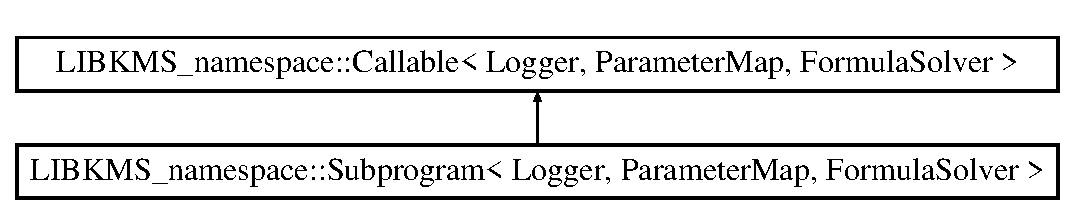
\includegraphics[height=2.000000cm]{classLIBKMS__namespace_1_1Subprogram}
\end{center}
\end{figure}
\subsection*{Классы}
\begin{DoxyCompactItemize}
\item 
struct \hyperlink{structLIBKMS__namespace_1_1Subprogram_1_1user__exception}{user\-\_\-exception}
\end{DoxyCompactItemize}
\subsection*{Открытые типы}
\begin{DoxyCompactItemize}
\item 
typedef Parameter\-Map \hyperlink{classLIBKMS__namespace_1_1Subprogram_a2ee2b32579888fcf68d85338b37b505c}{parameter\-\_\-map}
\item 
typedef \hyperlink{classLIBKMS__namespace_1_1FunctionStorage}{Function\-Storage}\\*
$<$ Parameter\-Map $>$ \hyperlink{classLIBKMS__namespace_1_1Subprogram_a6233a24c21954444f64217e7af397349}{function\-\_\-storage\-\_\-t}
\end{DoxyCompactItemize}
\subsection*{Открытые члены}
\begin{DoxyCompactItemize}
\item 
\hyperlink{classLIBKMS__namespace_1_1Callable_ad58caabaa5ac247c9d385e6d5451916a}{parameter\-\_\-map} \hyperlink{classLIBKMS__namespace_1_1Subprogram_a2898e1d2ff996ca6de8a0d6480be4e1f}{call} (double time, const \hyperlink{classLIBKMS__namespace_1_1Callable_ad58caabaa5ac247c9d385e6d5451916a}{parameter\-\_\-map} \&v, const \hyperlink{classLIBKMS__namespace_1_1Callable_ad58caabaa5ac247c9d385e6d5451916a}{parameter\-\_\-map} \&u)
\item 
\hyperlink{classLIBKMS__namespace_1_1Subprogram_a2279d8a886dbb2c16955e617c429b842}{Subprogram} (std\-::string name, std\-::string class\-\_\-, double priority)
\item 
bool \hyperlink{classLIBKMS__namespace_1_1Subprogram_ab147a59ea5ce42f20af207c3f1499fb0}{set\-\_\-key\-\_\-remap} (const param\-\_\-key\-\_\-t \&target, const param\-\_\-key\-\_\-t \&remapped)
\item 
bool \hyperlink{classLIBKMS__namespace_1_1Subprogram_a1c6cab2580663cd14f5297cfe6425ccd}{is\-\_\-func\-\_\-set} () const noexcept
\end{DoxyCompactItemize}
\subsection*{Дополнительные унаследованные члены}


\subsection{Подробное описание}
\subsubsection*{template$<$typename Logger, typename Parameter\-Map, typename Formula\-Solver$>$class L\-I\-B\-K\-M\-S\-\_\-namespace\-::\-Subprogram$<$ Logger, Parameter\-Map, Formula\-Solver $>$}

Шаблонный класс -\/ обертка подпрограмм 

\subsection{Определения типов}
\hypertarget{classLIBKMS__namespace_1_1Subprogram_a6233a24c21954444f64217e7af397349}{\index{L\-I\-B\-K\-M\-S\-\_\-namespace\-::\-Subprogram@{L\-I\-B\-K\-M\-S\-\_\-namespace\-::\-Subprogram}!function\-\_\-storage\-\_\-t@{function\-\_\-storage\-\_\-t}}
\index{function\-\_\-storage\-\_\-t@{function\-\_\-storage\-\_\-t}!LIBKMS_namespace::Subprogram@{L\-I\-B\-K\-M\-S\-\_\-namespace\-::\-Subprogram}}
\subsubsection[{function\-\_\-storage\-\_\-t}]{\setlength{\rightskip}{0pt plus 5cm}template$<$typename Logger , typename Parameter\-Map , typename Formula\-Solver $>$ typedef {\bf Function\-Storage}$<$ Parameter\-Map $>$ {\bf L\-I\-B\-K\-M\-S\-\_\-namespace\-::\-Subprogram}$<$ Logger, Parameter\-Map, Formula\-Solver $>$\-::{\bf function\-\_\-storage\-\_\-t}}}\label{classLIBKMS__namespace_1_1Subprogram_a6233a24c21954444f64217e7af397349}
\hypertarget{classLIBKMS__namespace_1_1Subprogram_a2ee2b32579888fcf68d85338b37b505c}{\index{L\-I\-B\-K\-M\-S\-\_\-namespace\-::\-Subprogram@{L\-I\-B\-K\-M\-S\-\_\-namespace\-::\-Subprogram}!parameter\-\_\-map@{parameter\-\_\-map}}
\index{parameter\-\_\-map@{parameter\-\_\-map}!LIBKMS_namespace::Subprogram@{L\-I\-B\-K\-M\-S\-\_\-namespace\-::\-Subprogram}}
\subsubsection[{parameter\-\_\-map}]{\setlength{\rightskip}{0pt plus 5cm}template$<$typename Logger , typename Parameter\-Map , typename Formula\-Solver $>$ typedef Parameter\-Map {\bf L\-I\-B\-K\-M\-S\-\_\-namespace\-::\-Subprogram}$<$ Logger, Parameter\-Map, Formula\-Solver $>$\-::{\bf parameter\-\_\-map}}}\label{classLIBKMS__namespace_1_1Subprogram_a2ee2b32579888fcf68d85338b37b505c}


\subsection{Конструктор(ы)}
\hypertarget{classLIBKMS__namespace_1_1Subprogram_a2279d8a886dbb2c16955e617c429b842}{\index{L\-I\-B\-K\-M\-S\-\_\-namespace\-::\-Subprogram@{L\-I\-B\-K\-M\-S\-\_\-namespace\-::\-Subprogram}!Subprogram@{Subprogram}}
\index{Subprogram@{Subprogram}!LIBKMS_namespace::Subprogram@{L\-I\-B\-K\-M\-S\-\_\-namespace\-::\-Subprogram}}
\subsubsection[{Subprogram}]{\setlength{\rightskip}{0pt plus 5cm}template$<$typename Logger , typename Parameter\-Map , typename Formula\-Solver $>$ {\bf L\-I\-B\-K\-M\-S\-\_\-namespace\-::\-Subprogram}$<$ Logger, Parameter\-Map, Formula\-Solver $>$\-::{\bf Subprogram} (
\begin{DoxyParamCaption}
\item[{std\-::string}]{name, }
\item[{std\-::string}]{class\-\_\-, }
\item[{double}]{priority}
\end{DoxyParamCaption}
)\hspace{0.3cm}{\ttfamily [inline]}}}\label{classLIBKMS__namespace_1_1Subprogram_a2279d8a886dbb2c16955e617c429b842}


\subsection{Методы}
\hypertarget{classLIBKMS__namespace_1_1Subprogram_a2898e1d2ff996ca6de8a0d6480be4e1f}{\index{L\-I\-B\-K\-M\-S\-\_\-namespace\-::\-Subprogram@{L\-I\-B\-K\-M\-S\-\_\-namespace\-::\-Subprogram}!call@{call}}
\index{call@{call}!LIBKMS_namespace::Subprogram@{L\-I\-B\-K\-M\-S\-\_\-namespace\-::\-Subprogram}}
\subsubsection[{call}]{\setlength{\rightskip}{0pt plus 5cm}template$<$typename Logger , typename Parameter\-Map , typename Formula\-Solver $>$ {\bf parameter\-\_\-map} {\bf L\-I\-B\-K\-M\-S\-\_\-namespace\-::\-Subprogram}$<$ Logger, Parameter\-Map, Formula\-Solver $>$\-::call (
\begin{DoxyParamCaption}
\item[{double}]{time, }
\item[{const {\bf parameter\-\_\-map} \&}]{block\-\_\-vars, }
\item[{const {\bf parameter\-\_\-map} \&}]{upper\-\_\-vars}
\end{DoxyParamCaption}
)\hspace{0.3cm}{\ttfamily [inline]}, {\ttfamily [virtual]}}}\label{classLIBKMS__namespace_1_1Subprogram_a2898e1d2ff996ca6de8a0d6480be4e1f}
Осуществить вызов объекта 
\begin{DoxyParams}{Аргументы}
{\em time} & текущее время \\
\hline
{\em block\-\_\-vars} & переменные родительского блока \\
\hline
{\em upper\-\_\-vars} & переменные родителя родительского блока \\
\hline
\end{DoxyParams}
\begin{DoxyReturn}{Возвращает}
новые значения для переменных родительского блока 
\end{DoxyReturn}


Замещает \hyperlink{classLIBKMS__namespace_1_1Callable_ad9cad480516a054f09c056ae248691b1}{L\-I\-B\-K\-M\-S\-\_\-namespace\-::\-Callable$<$ Logger, Parameter\-Map, Formula\-Solver $>$}.

\hypertarget{classLIBKMS__namespace_1_1Subprogram_a1c6cab2580663cd14f5297cfe6425ccd}{\index{L\-I\-B\-K\-M\-S\-\_\-namespace\-::\-Subprogram@{L\-I\-B\-K\-M\-S\-\_\-namespace\-::\-Subprogram}!is\-\_\-func\-\_\-set@{is\-\_\-func\-\_\-set}}
\index{is\-\_\-func\-\_\-set@{is\-\_\-func\-\_\-set}!LIBKMS_namespace::Subprogram@{L\-I\-B\-K\-M\-S\-\_\-namespace\-::\-Subprogram}}
\subsubsection[{is\-\_\-func\-\_\-set}]{\setlength{\rightskip}{0pt plus 5cm}template$<$typename Logger , typename Parameter\-Map , typename Formula\-Solver $>$ bool {\bf L\-I\-B\-K\-M\-S\-\_\-namespace\-::\-Subprogram}$<$ Logger, Parameter\-Map, Formula\-Solver $>$\-::is\-\_\-func\-\_\-set (
\begin{DoxyParamCaption}
{}
\end{DoxyParamCaption}
) const\hspace{0.3cm}{\ttfamily [inline]}, {\ttfamily [noexcept]}}}\label{classLIBKMS__namespace_1_1Subprogram_a1c6cab2580663cd14f5297cfe6425ccd}
\hypertarget{classLIBKMS__namespace_1_1Subprogram_ab147a59ea5ce42f20af207c3f1499fb0}{\index{L\-I\-B\-K\-M\-S\-\_\-namespace\-::\-Subprogram@{L\-I\-B\-K\-M\-S\-\_\-namespace\-::\-Subprogram}!set\-\_\-key\-\_\-remap@{set\-\_\-key\-\_\-remap}}
\index{set\-\_\-key\-\_\-remap@{set\-\_\-key\-\_\-remap}!LIBKMS_namespace::Subprogram@{L\-I\-B\-K\-M\-S\-\_\-namespace\-::\-Subprogram}}
\subsubsection[{set\-\_\-key\-\_\-remap}]{\setlength{\rightskip}{0pt plus 5cm}template$<$typename Logger , typename Parameter\-Map , typename Formula\-Solver $>$ bool {\bf L\-I\-B\-K\-M\-S\-\_\-namespace\-::\-Subprogram}$<$ Logger, Parameter\-Map, Formula\-Solver $>$\-::set\-\_\-key\-\_\-remap (
\begin{DoxyParamCaption}
\item[{const param\-\_\-key\-\_\-t \&}]{target, }
\item[{const param\-\_\-key\-\_\-t \&}]{remapped}
\end{DoxyParamCaption}
)\hspace{0.3cm}{\ttfamily [inline]}}}\label{classLIBKMS__namespace_1_1Subprogram_ab147a59ea5ce42f20af207c3f1499fb0}


Объявления и описания членов класса находятся в файле\-:\begin{DoxyCompactItemize}
\item 
\hyperlink{subprog_8hpp}{subprog.\-hpp}\end{DoxyCompactItemize}

\hypertarget{classLIBKMS__namespace_1_1TypeFactory}{\section{Шаблон класса L\-I\-B\-K\-M\-S\-\_\-namespace\-:\-:Type\-Factory$<$ Ext, Spec $>$}
\label{classLIBKMS__namespace_1_1TypeFactory}\index{L\-I\-B\-K\-M\-S\-\_\-namespace\-::\-Type\-Factory$<$ Ext, Spec $>$@{L\-I\-B\-K\-M\-S\-\_\-namespace\-::\-Type\-Factory$<$ Ext, Spec $>$}}
}


Фабрика параметров  




{\ttfamily \#include $<$typefactory.\-hpp$>$}

\subsection*{Открытые типы}
\begin{DoxyCompactItemize}
\item 
typedef \hyperlink{classLIBKMS__namespace_1_1TypeFactory}{Type\-Factory}$<$ Ext, Spec $>$ \hyperlink{classLIBKMS__namespace_1_1TypeFactory_a1ea3eb75810d29bed5a7f017e188a43d}{type\-\_\-factory\-\_\-t}
\item 
typedef \hyperlink{classLIBKMS__namespace_1_1Parameter}{Parameter}$<$ Ext, Spec $>$ \hyperlink{classLIBKMS__namespace_1_1TypeFactory_a103a08b747cfe5b233b12c802b4563dc}{parameter\-\_\-t}
\item 
typedef \hyperlink{classLIBKMS__namespace_1_1Parameter_a28516bcd5bad5857b2d1c676e4176f51}{parameter\-\_\-t\-::ptr\-\_\-t} \hyperlink{classLIBKMS__namespace_1_1TypeFactory_a54c61c4d970a37a1059746070a1eea11}{parameter\-\_\-ptr}
\item 
typedef \hyperlink{classLIBKMS__namespace_1_1Holder}{Holder}\\*
$<$ std\-\_\-types\-::t\-Bool, \\*
\hyperlink{classLIBKMS__namespace_1_1TypeFactory_a103a08b747cfe5b233b12c802b4563dc}{parameter\-\_\-t} $>$ \hyperlink{classLIBKMS__namespace_1_1TypeFactory_a5af2bfe6425fe90d4951268240dc1768}{bool\-\_\-holder}
\item 
typedef \hyperlink{classLIBKMS__namespace_1_1Holder}{Holder}\\*
$<$ std\-\_\-types\-::t\-Int, \hyperlink{classLIBKMS__namespace_1_1TypeFactory_a103a08b747cfe5b233b12c802b4563dc}{parameter\-\_\-t} $>$ \hyperlink{classLIBKMS__namespace_1_1TypeFactory_a118a2227ad78008ae8e7d16c9d7f854a}{int\-\_\-holder}
\item 
typedef \hyperlink{classLIBKMS__namespace_1_1Holder}{Holder}\\*
$<$ std\-\_\-types\-::t\-Real, \\*
\hyperlink{classLIBKMS__namespace_1_1TypeFactory_a103a08b747cfe5b233b12c802b4563dc}{parameter\-\_\-t} $>$ \hyperlink{classLIBKMS__namespace_1_1TypeFactory_a789fcb94a8ce6dfd8b2ff0e9b4ce299c}{real\-\_\-holder}
\item 
typedef \hyperlink{classLIBKMS__namespace_1_1Holder}{Holder}\\*
$<$ std\-\_\-types\-::t\-String, \\*
\hyperlink{classLIBKMS__namespace_1_1TypeFactory_a103a08b747cfe5b233b12c802b4563dc}{parameter\-\_\-t} $>$ \hyperlink{classLIBKMS__namespace_1_1TypeFactory_a17b132ee9e501536bec342ed6377497a}{string\-\_\-holder}
\end{DoxyCompactItemize}
\subsection*{Открытые члены}
\begin{DoxyCompactItemize}
\item 
\hyperlink{classLIBKMS__namespace_1_1TypeFactory_a54c61c4d970a37a1059746070a1eea11}{parameter\-\_\-ptr} \hyperlink{classLIBKMS__namespace_1_1TypeFactory_a5105b6ca3256a95cebe301c14e8f56dc}{create} (const std\-::string \&name) const noexcept
\item 
{\footnotesize template$<$typename T $>$ }\\void \hyperlink{classLIBKMS__namespace_1_1TypeFactory_ac4c8b3e60558d8402e8a405cab8c1079}{add\-\_\-type} (const std\-::string \&name)
\end{DoxyCompactItemize}
\subsection*{Открытые статические члены}
\begin{DoxyCompactItemize}
\item 
static \hyperlink{classLIBKMS__namespace_1_1TypeFactory_a1ea3eb75810d29bed5a7f017e188a43d}{type\-\_\-factory\-\_\-t} \& \hyperlink{classLIBKMS__namespace_1_1TypeFactory_a14d95fd9ad1442a0c10120519f9841d7}{instance} () noexcept
\end{DoxyCompactItemize}


\subsection{Подробное описание}
\subsubsection*{template$<$typename Ext, template$<$ typename U $>$ class Spec$>$class L\-I\-B\-K\-M\-S\-\_\-namespace\-::\-Type\-Factory$<$ Ext, Spec $>$}

Фабрика параметров 

\subsection{Определения типов}
\hypertarget{classLIBKMS__namespace_1_1TypeFactory_a5af2bfe6425fe90d4951268240dc1768}{\index{L\-I\-B\-K\-M\-S\-\_\-namespace\-::\-Type\-Factory@{L\-I\-B\-K\-M\-S\-\_\-namespace\-::\-Type\-Factory}!bool\-\_\-holder@{bool\-\_\-holder}}
\index{bool\-\_\-holder@{bool\-\_\-holder}!LIBKMS_namespace::TypeFactory@{L\-I\-B\-K\-M\-S\-\_\-namespace\-::\-Type\-Factory}}
\subsubsection[{bool\-\_\-holder}]{\setlength{\rightskip}{0pt plus 5cm}template$<$typename Ext , template$<$ typename U $>$ class Spec$>$ typedef {\bf Holder}$<$ std\-\_\-types\-::t\-Bool, {\bf parameter\-\_\-t} $>$ {\bf L\-I\-B\-K\-M\-S\-\_\-namespace\-::\-Type\-Factory}$<$ Ext, Spec $>$\-::{\bf bool\-\_\-holder}}}\label{classLIBKMS__namespace_1_1TypeFactory_a5af2bfe6425fe90d4951268240dc1768}
\hypertarget{classLIBKMS__namespace_1_1TypeFactory_a118a2227ad78008ae8e7d16c9d7f854a}{\index{L\-I\-B\-K\-M\-S\-\_\-namespace\-::\-Type\-Factory@{L\-I\-B\-K\-M\-S\-\_\-namespace\-::\-Type\-Factory}!int\-\_\-holder@{int\-\_\-holder}}
\index{int\-\_\-holder@{int\-\_\-holder}!LIBKMS_namespace::TypeFactory@{L\-I\-B\-K\-M\-S\-\_\-namespace\-::\-Type\-Factory}}
\subsubsection[{int\-\_\-holder}]{\setlength{\rightskip}{0pt plus 5cm}template$<$typename Ext , template$<$ typename U $>$ class Spec$>$ typedef {\bf Holder}$<$ std\-\_\-types\-::t\-Int, {\bf parameter\-\_\-t} $>$ {\bf L\-I\-B\-K\-M\-S\-\_\-namespace\-::\-Type\-Factory}$<$ Ext, Spec $>$\-::{\bf int\-\_\-holder}}}\label{classLIBKMS__namespace_1_1TypeFactory_a118a2227ad78008ae8e7d16c9d7f854a}
\hypertarget{classLIBKMS__namespace_1_1TypeFactory_a54c61c4d970a37a1059746070a1eea11}{\index{L\-I\-B\-K\-M\-S\-\_\-namespace\-::\-Type\-Factory@{L\-I\-B\-K\-M\-S\-\_\-namespace\-::\-Type\-Factory}!parameter\-\_\-ptr@{parameter\-\_\-ptr}}
\index{parameter\-\_\-ptr@{parameter\-\_\-ptr}!LIBKMS_namespace::TypeFactory@{L\-I\-B\-K\-M\-S\-\_\-namespace\-::\-Type\-Factory}}
\subsubsection[{parameter\-\_\-ptr}]{\setlength{\rightskip}{0pt plus 5cm}template$<$typename Ext , template$<$ typename U $>$ class Spec$>$ typedef {\bf parameter\-\_\-t\-::ptr\-\_\-t} {\bf L\-I\-B\-K\-M\-S\-\_\-namespace\-::\-Type\-Factory}$<$ Ext, Spec $>$\-::{\bf parameter\-\_\-ptr}}}\label{classLIBKMS__namespace_1_1TypeFactory_a54c61c4d970a37a1059746070a1eea11}
\hypertarget{classLIBKMS__namespace_1_1TypeFactory_a103a08b747cfe5b233b12c802b4563dc}{\index{L\-I\-B\-K\-M\-S\-\_\-namespace\-::\-Type\-Factory@{L\-I\-B\-K\-M\-S\-\_\-namespace\-::\-Type\-Factory}!parameter\-\_\-t@{parameter\-\_\-t}}
\index{parameter\-\_\-t@{parameter\-\_\-t}!LIBKMS_namespace::TypeFactory@{L\-I\-B\-K\-M\-S\-\_\-namespace\-::\-Type\-Factory}}
\subsubsection[{parameter\-\_\-t}]{\setlength{\rightskip}{0pt plus 5cm}template$<$typename Ext , template$<$ typename U $>$ class Spec$>$ typedef {\bf Parameter}$<$ Ext, Spec $>$ {\bf L\-I\-B\-K\-M\-S\-\_\-namespace\-::\-Type\-Factory}$<$ Ext, Spec $>$\-::{\bf parameter\-\_\-t}}}\label{classLIBKMS__namespace_1_1TypeFactory_a103a08b747cfe5b233b12c802b4563dc}
\hypertarget{classLIBKMS__namespace_1_1TypeFactory_a789fcb94a8ce6dfd8b2ff0e9b4ce299c}{\index{L\-I\-B\-K\-M\-S\-\_\-namespace\-::\-Type\-Factory@{L\-I\-B\-K\-M\-S\-\_\-namespace\-::\-Type\-Factory}!real\-\_\-holder@{real\-\_\-holder}}
\index{real\-\_\-holder@{real\-\_\-holder}!LIBKMS_namespace::TypeFactory@{L\-I\-B\-K\-M\-S\-\_\-namespace\-::\-Type\-Factory}}
\subsubsection[{real\-\_\-holder}]{\setlength{\rightskip}{0pt plus 5cm}template$<$typename Ext , template$<$ typename U $>$ class Spec$>$ typedef {\bf Holder}$<$ std\-\_\-types\-::t\-Real, {\bf parameter\-\_\-t} $>$ {\bf L\-I\-B\-K\-M\-S\-\_\-namespace\-::\-Type\-Factory}$<$ Ext, Spec $>$\-::{\bf real\-\_\-holder}}}\label{classLIBKMS__namespace_1_1TypeFactory_a789fcb94a8ce6dfd8b2ff0e9b4ce299c}
\hypertarget{classLIBKMS__namespace_1_1TypeFactory_a17b132ee9e501536bec342ed6377497a}{\index{L\-I\-B\-K\-M\-S\-\_\-namespace\-::\-Type\-Factory@{L\-I\-B\-K\-M\-S\-\_\-namespace\-::\-Type\-Factory}!string\-\_\-holder@{string\-\_\-holder}}
\index{string\-\_\-holder@{string\-\_\-holder}!LIBKMS_namespace::TypeFactory@{L\-I\-B\-K\-M\-S\-\_\-namespace\-::\-Type\-Factory}}
\subsubsection[{string\-\_\-holder}]{\setlength{\rightskip}{0pt plus 5cm}template$<$typename Ext , template$<$ typename U $>$ class Spec$>$ typedef {\bf Holder}$<$ std\-\_\-types\-::t\-String, {\bf parameter\-\_\-t} $>$ {\bf L\-I\-B\-K\-M\-S\-\_\-namespace\-::\-Type\-Factory}$<$ Ext, Spec $>$\-::{\bf string\-\_\-holder}}}\label{classLIBKMS__namespace_1_1TypeFactory_a17b132ee9e501536bec342ed6377497a}
\hypertarget{classLIBKMS__namespace_1_1TypeFactory_a1ea3eb75810d29bed5a7f017e188a43d}{\index{L\-I\-B\-K\-M\-S\-\_\-namespace\-::\-Type\-Factory@{L\-I\-B\-K\-M\-S\-\_\-namespace\-::\-Type\-Factory}!type\-\_\-factory\-\_\-t@{type\-\_\-factory\-\_\-t}}
\index{type\-\_\-factory\-\_\-t@{type\-\_\-factory\-\_\-t}!LIBKMS_namespace::TypeFactory@{L\-I\-B\-K\-M\-S\-\_\-namespace\-::\-Type\-Factory}}
\subsubsection[{type\-\_\-factory\-\_\-t}]{\setlength{\rightskip}{0pt plus 5cm}template$<$typename Ext , template$<$ typename U $>$ class Spec$>$ typedef {\bf Type\-Factory}$<$ Ext, Spec $>$ {\bf L\-I\-B\-K\-M\-S\-\_\-namespace\-::\-Type\-Factory}$<$ Ext, Spec $>$\-::{\bf type\-\_\-factory\-\_\-t}}}\label{classLIBKMS__namespace_1_1TypeFactory_a1ea3eb75810d29bed5a7f017e188a43d}


\subsection{Методы}
\hypertarget{classLIBKMS__namespace_1_1TypeFactory_ac4c8b3e60558d8402e8a405cab8c1079}{\index{L\-I\-B\-K\-M\-S\-\_\-namespace\-::\-Type\-Factory@{L\-I\-B\-K\-M\-S\-\_\-namespace\-::\-Type\-Factory}!add\-\_\-type@{add\-\_\-type}}
\index{add\-\_\-type@{add\-\_\-type}!LIBKMS_namespace::TypeFactory@{L\-I\-B\-K\-M\-S\-\_\-namespace\-::\-Type\-Factory}}
\subsubsection[{add\-\_\-type}]{\setlength{\rightskip}{0pt plus 5cm}template$<$typename Ext , template$<$ typename U $>$ class Spec$>$ template$<$typename T $>$ void {\bf L\-I\-B\-K\-M\-S\-\_\-namespace\-::\-Type\-Factory}$<$ Ext, Spec $>$\-::add\-\_\-type (
\begin{DoxyParamCaption}
\item[{const std\-::string \&}]{name}
\end{DoxyParamCaption}
)\hspace{0.3cm}{\ttfamily [inline]}}}\label{classLIBKMS__namespace_1_1TypeFactory_ac4c8b3e60558d8402e8a405cab8c1079}
\hypertarget{classLIBKMS__namespace_1_1TypeFactory_a5105b6ca3256a95cebe301c14e8f56dc}{\index{L\-I\-B\-K\-M\-S\-\_\-namespace\-::\-Type\-Factory@{L\-I\-B\-K\-M\-S\-\_\-namespace\-::\-Type\-Factory}!create@{create}}
\index{create@{create}!LIBKMS_namespace::TypeFactory@{L\-I\-B\-K\-M\-S\-\_\-namespace\-::\-Type\-Factory}}
\subsubsection[{create}]{\setlength{\rightskip}{0pt plus 5cm}template$<$typename Ext , template$<$ typename U $>$ class Spec$>$ {\bf parameter\-\_\-ptr} {\bf L\-I\-B\-K\-M\-S\-\_\-namespace\-::\-Type\-Factory}$<$ Ext, Spec $>$\-::create (
\begin{DoxyParamCaption}
\item[{const std\-::string \&}]{name}
\end{DoxyParamCaption}
) const\hspace{0.3cm}{\ttfamily [inline]}, {\ttfamily [noexcept]}}}\label{classLIBKMS__namespace_1_1TypeFactory_a5105b6ca3256a95cebe301c14e8f56dc}
\hypertarget{classLIBKMS__namespace_1_1TypeFactory_a14d95fd9ad1442a0c10120519f9841d7}{\index{L\-I\-B\-K\-M\-S\-\_\-namespace\-::\-Type\-Factory@{L\-I\-B\-K\-M\-S\-\_\-namespace\-::\-Type\-Factory}!instance@{instance}}
\index{instance@{instance}!LIBKMS_namespace::TypeFactory@{L\-I\-B\-K\-M\-S\-\_\-namespace\-::\-Type\-Factory}}
\subsubsection[{instance}]{\setlength{\rightskip}{0pt plus 5cm}template$<$typename Ext , template$<$ typename U $>$ class Spec$>$ static {\bf type\-\_\-factory\-\_\-t}\& {\bf L\-I\-B\-K\-M\-S\-\_\-namespace\-::\-Type\-Factory}$<$ Ext, Spec $>$\-::instance (
\begin{DoxyParamCaption}
{}
\end{DoxyParamCaption}
)\hspace{0.3cm}{\ttfamily [inline]}, {\ttfamily [static]}, {\ttfamily [noexcept]}}}\label{classLIBKMS__namespace_1_1TypeFactory_a14d95fd9ad1442a0c10120519f9841d7}


Объявления и описания членов класса находятся в файле\-:\begin{DoxyCompactItemize}
\item 
\hyperlink{typefactory_8hpp}{typefactory.\-hpp}\end{DoxyCompactItemize}

\hypertarget{structLIBKMS__namespace_1_1Subprogram_1_1user__exception}{\section{Структура L\-I\-B\-K\-M\-S\-\_\-namespace\-:\-:Subprogram$<$ Logger, Parameter\-Map, Formula\-Solver $>$\-:\-:user\-\_\-exception}
\label{structLIBKMS__namespace_1_1Subprogram_1_1user__exception}\index{L\-I\-B\-K\-M\-S\-\_\-namespace\-::\-Subprogram$<$ Logger, Parameter\-Map, Formula\-Solver $>$\-::user\-\_\-exception@{L\-I\-B\-K\-M\-S\-\_\-namespace\-::\-Subprogram$<$ Logger, Parameter\-Map, Formula\-Solver $>$\-::user\-\_\-exception}}
}


{\ttfamily \#include $<$subprog.\-hpp$>$}

Граф наследования\-:L\-I\-B\-K\-M\-S\-\_\-namespace\-:\-:Subprogram$<$ Logger, Parameter\-Map, Formula\-Solver $>$\-:\-:user\-\_\-exception\-:\begin{figure}[H]
\begin{center}
\leavevmode
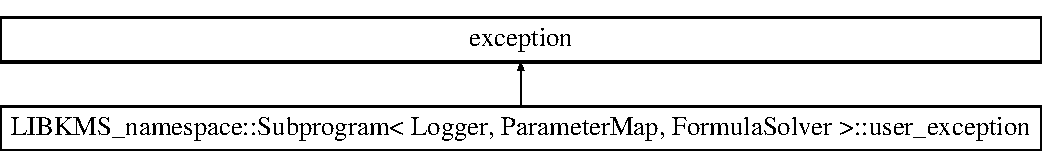
\includegraphics[height=2.000000cm]{structLIBKMS__namespace_1_1Subprogram_1_1user__exception}
\end{center}
\end{figure}
\subsection*{Открытые члены}
\begin{DoxyCompactItemize}
\item 
\hyperlink{structLIBKMS__namespace_1_1Subprogram_1_1user__exception_ae95b23bd4a15dfcd4d465523ccb3fee3}{user\-\_\-exception} (const std\-::string \&data, const std\-::string \&desc)
\item 
const char $\ast$ \hyperlink{structLIBKMS__namespace_1_1Subprogram_1_1user__exception_a3ba2886c83dd09d8b75da56c1145f76b}{what} () const noexcept
\end{DoxyCompactItemize}


\subsection{Конструктор(ы)}
\hypertarget{structLIBKMS__namespace_1_1Subprogram_1_1user__exception_ae95b23bd4a15dfcd4d465523ccb3fee3}{\index{L\-I\-B\-K\-M\-S\-\_\-namespace\-::\-Subprogram\-::user\-\_\-exception@{L\-I\-B\-K\-M\-S\-\_\-namespace\-::\-Subprogram\-::user\-\_\-exception}!user\-\_\-exception@{user\-\_\-exception}}
\index{user\-\_\-exception@{user\-\_\-exception}!LIBKMS_namespace::Subprogram::user_exception@{L\-I\-B\-K\-M\-S\-\_\-namespace\-::\-Subprogram\-::user\-\_\-exception}}
\subsubsection[{user\-\_\-exception}]{\setlength{\rightskip}{0pt plus 5cm}template$<$typename Logger , typename Parameter\-Map , typename Formula\-Solver $>$ {\bf L\-I\-B\-K\-M\-S\-\_\-namespace\-::\-Subprogram}$<$ Logger, Parameter\-Map, Formula\-Solver $>$\-::user\-\_\-exception\-::user\-\_\-exception (
\begin{DoxyParamCaption}
\item[{const std\-::string \&}]{data, }
\item[{const std\-::string \&}]{desc}
\end{DoxyParamCaption}
)\hspace{0.3cm}{\ttfamily [inline]}}}\label{structLIBKMS__namespace_1_1Subprogram_1_1user__exception_ae95b23bd4a15dfcd4d465523ccb3fee3}


\subsection{Методы}
\hypertarget{structLIBKMS__namespace_1_1Subprogram_1_1user__exception_a3ba2886c83dd09d8b75da56c1145f76b}{\index{L\-I\-B\-K\-M\-S\-\_\-namespace\-::\-Subprogram\-::user\-\_\-exception@{L\-I\-B\-K\-M\-S\-\_\-namespace\-::\-Subprogram\-::user\-\_\-exception}!what@{what}}
\index{what@{what}!LIBKMS_namespace::Subprogram::user_exception@{L\-I\-B\-K\-M\-S\-\_\-namespace\-::\-Subprogram\-::user\-\_\-exception}}
\subsubsection[{what}]{\setlength{\rightskip}{0pt plus 5cm}template$<$typename Logger , typename Parameter\-Map , typename Formula\-Solver $>$ const char$\ast$ {\bf L\-I\-B\-K\-M\-S\-\_\-namespace\-::\-Subprogram}$<$ Logger, Parameter\-Map, Formula\-Solver $>$\-::user\-\_\-exception\-::what (
\begin{DoxyParamCaption}
{}
\end{DoxyParamCaption}
) const\hspace{0.3cm}{\ttfamily [inline]}, {\ttfamily [noexcept]}}}\label{structLIBKMS__namespace_1_1Subprogram_1_1user__exception_a3ba2886c83dd09d8b75da56c1145f76b}


Объявления и описания членов структуры находятся в файле\-:\begin{DoxyCompactItemize}
\item 
\hyperlink{subprog_8hpp}{subprog.\-hpp}\end{DoxyCompactItemize}

\chapter{Файлы}
\hypertarget{block_8hpp}{\section{Файл block.\-hpp}
\label{block_8hpp}\index{block.\-hpp@{block.\-hpp}}
}
{\ttfamily \#include $<$block\-\_\-class.\-hpp$>$}\\*
{\ttfamily \#include $<$callable.\-hpp$>$}\\*
{\ttfamily \#include $<$detail/spec.\-hpp$>$}\\*
{\ttfamily \#include $<$detail/std.\-hpp$>$}\\*
{\ttfamily \#include $<$set$>$}\\*
\subsection*{Классы}
\begin{DoxyCompactItemize}
\item 
class \hyperlink{classLIBKMS__namespace_1_1Block}{L\-I\-B\-K\-M\-S\-\_\-namespace\-::\-Block$<$ Type\-Factory, Param\-Spec, Scheduler, Logger, Subpr\-Spec, String\-Spec, Bl\-Cl\-Spec, Formula\-Solver $>$}
\begin{DoxyCompactList}\small\item\em Шаблонный класс \hyperlink{classLIBKMS__namespace_1_1Block}{Block}, отображающий блок процесс. \end{DoxyCompactList}\end{DoxyCompactItemize}
\subsection*{Пространства имен}
\begin{DoxyCompactItemize}
\item 
\hyperlink{namespaceLIBKMS__namespace}{L\-I\-B\-K\-M\-S\-\_\-namespace}
\end{DoxyCompactItemize}

\hypertarget{block__class_8hpp}{\section{Файл block\-\_\-class.\-hpp}
\label{block__class_8hpp}\index{block\-\_\-class.\-hpp@{block\-\_\-class.\-hpp}}
}
{\ttfamily \#include $<$block\-\_\-class/names.\-hpp$>$}\\*
{\ttfamily \#include $<$limits$>$}\\*
{\ttfamily \#include $<$string$>$}\\*
{\ttfamily \#include $<$sstream$>$}\\*
{\ttfamily \#include $<$block\-\_\-class/udp\-\_\-exchange.\-hpp$>$}\\*
\subsection*{Классы}
\begin{DoxyCompactItemize}
\item 
class \hyperlink{classLIBKMS__namespace_1_1BlockClass}{L\-I\-B\-K\-M\-S\-\_\-namespace\-::\-Block\-Class$<$ Function\-Storage, Subprogram, Subprogram\-Ptr, Block\-Ptr, Bl\-Cl\-Spec $>$}
\begin{DoxyCompactList}\small\item\em Прототип описания класса блока \end{DoxyCompactList}\item 
struct \hyperlink{structLIBKMS__namespace_1_1BlockClassWithConfig}{L\-I\-B\-K\-M\-S\-\_\-namespace\-::\-Block\-Class\-With\-Config$<$ Function\-Storage, Subprogram, Subprogram\-Ptr, Block\-Ptr, Config\-Node, Bl\-Cl\-Spec $>$}
\item 
class \hyperlink{classLIBKMS__namespace_1_1BlockClassFactory}{L\-I\-B\-K\-M\-S\-\_\-namespace\-::\-Block\-Class\-Factory$<$ Function\-Storage, Subprogram, Subprogram\-Ptr, Block\-Ptr, Bl\-Cl\-Spec $>$}
\begin{DoxyCompactList}\small\item\em Фабрика классов блоков \end{DoxyCompactList}\item 
struct \hyperlink{structLIBKMS__namespace_1_1BlockClassFactory_1_1block__class__with__config}{L\-I\-B\-K\-M\-S\-\_\-namespace\-::\-Block\-Class\-Factory$<$ Function\-Storage, Subprogram, Subprogram\-Ptr, Block\-Ptr, Bl\-Cl\-Spec $>$\-::block\-\_\-class\-\_\-with\-\_\-config$<$ T $>$}
\end{DoxyCompactItemize}
\subsection*{Пространства имен}
\begin{DoxyCompactItemize}
\item 
\hyperlink{namespaceLIBKMS__namespace}{L\-I\-B\-K\-M\-S\-\_\-namespace}
\end{DoxyCompactItemize}

\hypertarget{callable_8hpp}{\section{Файл callable.\-hpp}
\label{callable_8hpp}\index{callable.\-hpp@{callable.\-hpp}}
}
{\ttfamily \#include $<$string$>$}\\*
{\ttfamily \#include $<$list$>$}\\*
{\ttfamily \#include $<$vector$>$}\\*
{\ttfamily \#include $<$boost/date\-\_\-time/posix\-\_\-time/posix\-\_\-time.\-hpp$>$}\\*
\subsection*{Классы}
\begin{DoxyCompactItemize}
\item 
class \hyperlink{classLIBKMS__namespace_1_1Callable}{L\-I\-B\-K\-M\-S\-\_\-namespace\-::\-Callable$<$ Logger, Parameter\-Map, Formula\-Solver $>$}
\end{DoxyCompactItemize}
\subsection*{Пространства имен}
\begin{DoxyCompactItemize}
\item 
\hyperlink{namespaceLIBKMS__namespace}{L\-I\-B\-K\-M\-S\-\_\-namespace}
\end{DoxyCompactItemize}

\hypertarget{class__spec_8hpp}{\section{Файл class\-\_\-spec.\-hpp}
\label{class__spec_8hpp}\index{class\-\_\-spec.\-hpp@{class\-\_\-spec.\-hpp}}
}
{\ttfamily \#include $<$detail/fwd.\-hpp$>$}\\*
{\ttfamily \#include $<$detail/std.\-hpp$>$}\\*
{\ttfamily \#include $<$detail/std\-\_\-types.\-hpp$>$}\\*
{\ttfamily \#include $<$detail/spec.\-hpp$>$}\\*
\subsection*{Классы}
\begin{DoxyCompactItemize}
\item 
struct \hyperlink{structLIBKMS__namespace_1_1class__spec}{L\-I\-B\-K\-M\-S\-\_\-namespace\-::class\-\_\-spec$<$ Param\-Ext, Param\-Spec, Scheduler, Logger, Subpr\-Spec, String\-Spec, Block\-Class\-Spec, Power\-On\-Formula\-Solver $>$}
\item 
struct \hyperlink{structLIBKMS__namespace_1_1class__spec_1_1holder}{L\-I\-B\-K\-M\-S\-\_\-namespace\-::class\-\_\-spec$<$ Param\-Ext, Param\-Spec, Scheduler, Logger, Subpr\-Spec, String\-Spec, Block\-Class\-Spec, Power\-On\-Formula\-Solver $>$\-::holder$<$ T $>$}
\end{DoxyCompactItemize}
\subsection*{Пространства имен}
\begin{DoxyCompactItemize}
\item 
\hyperlink{namespaceLIBKMS__namespace}{L\-I\-B\-K\-M\-S\-\_\-namespace}
\end{DoxyCompactItemize}
\subsection*{Определения типов}
\begin{DoxyCompactItemize}
\item 
typedef class\-\_\-spec\\*
$<$ No\-Extension, \\*
remappable\-\_\-shared\-\_\-ptr\-\_\-spec, \\*
Std\-Scheduler$<$ Std\-Logger $>$\\*
, Std\-Logger, shared\-\_\-ptr\-\_\-spec, \\*
Std\-String\-Spec, shared\-\_\-ptr\-\_\-spec, \\*
Std\-Power\-On\-Formula\-Solver $>$ \hyperlink{namespaceLIBKMS__namespace_ae7952b6893ea0986997f67d2945fc1a1}{L\-I\-B\-K\-M\-S\-\_\-namespace\-::std\-\_\-class\-\_\-spec}
\begin{DoxyCompactList}\small\item\em Стандартная специализация для шаблона \end{DoxyCompactList}\end{DoxyCompactItemize}

\hypertarget{control__func_8hpp}{\section{Файл control\-\_\-func.\-hpp}
\label{control__func_8hpp}\index{control\-\_\-func.\-hpp@{control\-\_\-func.\-hpp}}
}
{\ttfamily \#include $<$detail/spec.\-hpp$>$}\\*
{\ttfamily \#include $<$string$>$}\\*
{\ttfamily \#include $<$vector$>$}\\*
{\ttfamily \#include $<$sstream$>$}\\*
\subsection*{Классы}
\begin{DoxyCompactItemize}
\item 
class \hyperlink{classLIBKMS__namespace_1_1ControlFunc}{L\-I\-B\-K\-M\-S\-\_\-namespace\-::\-Control\-Func$<$ Type\-Factory, Block\-Ptr, Logger $>$}
\begin{DoxyCompactList}\small\item\em Шаблон класса \char`\"{}управляющая функция\char`\"{} (ФИ) \end{DoxyCompactList}\item 
class \hyperlink{classLIBKMS__namespace_1_1ControlFuncStorage}{L\-I\-B\-K\-M\-S\-\_\-namespace\-::\-Control\-Func\-Storage$<$ Type\-Factory, Block\-Ptr, Logger, Spec $>$}
\end{DoxyCompactItemize}
\subsection*{Пространства имен}
\begin{DoxyCompactItemize}
\item 
\hyperlink{namespaceLIBKMS__namespace}{L\-I\-B\-K\-M\-S\-\_\-namespace}
\end{DoxyCompactItemize}

\hypertarget{function__storage_8hpp}{\section{Файл function\-\_\-storage.\-hpp}
\label{function__storage_8hpp}\index{function\-\_\-storage.\-hpp@{function\-\_\-storage.\-hpp}}
}
{\ttfamily \#include $<$map$>$}\\*
{\ttfamily \#include $<$string$>$}\\*
{\ttfamily \#include $<$functional$>$}\\*
\subsection*{Классы}
\begin{DoxyCompactItemize}
\item 
class \hyperlink{classLIBKMS__namespace_1_1FunctionStorage}{L\-I\-B\-K\-M\-S\-\_\-namespace\-::\-Function\-Storage$<$ Parameter\-Map $>$}
\begin{DoxyCompactList}\small\item\em Фабрика подпрограмм \end{DoxyCompactList}\end{DoxyCompactItemize}
\subsection*{Пространства имен}
\begin{DoxyCompactItemize}
\item 
\hyperlink{namespaceLIBKMS__namespace}{L\-I\-B\-K\-M\-S\-\_\-namespace}
\end{DoxyCompactItemize}

\hypertarget{holder_8hpp}{\section{Файл holder.\-hpp}
\label{holder_8hpp}\index{holder.\-hpp@{holder.\-hpp}}
}
{\ttfamily \#include $<$param.\-hpp$>$}\\*
{\ttfamily \#include $<$param/convert.\-hpp$>$}\\*
{\ttfamily \#include $<$detail/fwd.\-hpp$>$}\\*
{\ttfamily \#include $<$detail/std\-\_\-types.\-hpp$>$}\\*
{\ttfamily \#include $<$sstream$>$}\\*
{\ttfamily \#include $<$string$>$}\\*
{\ttfamily \#include $<$iostream$>$}\\*
{\ttfamily \#include $<$cstring$>$}\\*
\subsection*{Классы}
\begin{DoxyCompactItemize}
\item 
struct \hyperlink{structLIBKMS__namespace_1_1obj__as_3_01Holder_3_01T_00_01P_01_4_00_01P_01_4}{L\-I\-B\-K\-M\-S\-\_\-namespace\-::obj\-\_\-as$<$ Holder$<$ T, P $>$, P $>$}
\begin{DoxyCompactList}\small\item\em Специализация для преобразования parameter в Holder$<$ T $>$ \end{DoxyCompactList}\item 
class \hyperlink{classLIBKMS__namespace_1_1Holder}{L\-I\-B\-K\-M\-S\-\_\-namespace\-::\-Holder$<$ T, Parameter $>$}
\begin{DoxyCompactList}\small\item\em Класс-\/контейнер для стандартных типов \end{DoxyCompactList}\item 
struct \hyperlink{structLIBKMS__namespace_1_1types_1_1get__return__type_3_01std__types_1_1tBool_00_01P_01_4}{L\-I\-B\-K\-M\-S\-\_\-namespace\-::types\-::get\-\_\-return\-\_\-type$<$ std\-\_\-types\-::t\-Bool, P $>$}
\item 
struct \hyperlink{structLIBKMS__namespace_1_1types_1_1get__return__type_3_01std__types_1_1tInt_00_01P_01_4}{L\-I\-B\-K\-M\-S\-\_\-namespace\-::types\-::get\-\_\-return\-\_\-type$<$ std\-\_\-types\-::t\-Int, P $>$}
\item 
struct \hyperlink{structLIBKMS__namespace_1_1types_1_1get__return__type_3_01std__types_1_1tReal_00_01P_01_4}{L\-I\-B\-K\-M\-S\-\_\-namespace\-::types\-::get\-\_\-return\-\_\-type$<$ std\-\_\-types\-::t\-Real, P $>$}
\item 
struct \hyperlink{structLIBKMS__namespace_1_1types_1_1get__return__type_3_01std__types_1_1tString_00_01P_01_4}{L\-I\-B\-K\-M\-S\-\_\-namespace\-::types\-::get\-\_\-return\-\_\-type$<$ std\-\_\-types\-::t\-String, P $>$}
\item 
class \hyperlink{classLIBKMS__namespace_1_1exception_1_1invalid__var__name}{L\-I\-B\-K\-M\-S\-\_\-namespace\-::exception\-::invalid\-\_\-var\-\_\-name}
\item 
class \hyperlink{classLIBKMS__namespace_1_1exception_1_1invalid__type}{L\-I\-B\-K\-M\-S\-\_\-namespace\-::exception\-::invalid\-\_\-type}
\item 
struct \hyperlink{structLIBKMS__namespace_1_1map__tools_1_1get}{L\-I\-B\-K\-M\-S\-\_\-namespace\-::map\-\_\-tools\-::get$<$ T $>$}
\begin{DoxyCompactList}\small\item\em Извлечь параметр определенного типа из шаблона \end{DoxyCompactList}\end{DoxyCompactItemize}
\subsection*{Пространства имен}
\begin{DoxyCompactItemize}
\item 
\hyperlink{namespaceLIBKMS__namespace}{L\-I\-B\-K\-M\-S\-\_\-namespace}
\item 
\hyperlink{namespaceLIBKMS__namespace_1_1holder__util}{L\-I\-B\-K\-M\-S\-\_\-namespace\-::holder\-\_\-util}
\item 
\hyperlink{namespaceLIBKMS__namespace_1_1types}{L\-I\-B\-K\-M\-S\-\_\-namespace\-::types}
\item 
\hyperlink{namespaceLIBKMS__namespace_1_1exception}{L\-I\-B\-K\-M\-S\-\_\-namespace\-::exception}
\item 
\hyperlink{namespaceLIBKMS__namespace_1_1map__tools}{L\-I\-B\-K\-M\-S\-\_\-namespace\-::map\-\_\-tools}
\end{DoxyCompactItemize}
\subsection*{Функции}
\begin{DoxyCompactItemize}
\item 
{\footnotesize template$<$typename T $>$ }\\std\-::string \hyperlink{namespaceLIBKMS__namespace_1_1holder__util_a3f905fcf57ce738c4f3a82676d0cf590}{L\-I\-B\-K\-M\-S\-\_\-namespace\-::holder\-\_\-util\-::to\-\_\-string} (const T \&m)
\begin{DoxyCompactList}\small\item\em Шаблон функции для печати данных в строку \end{DoxyCompactList}\item 
{\footnotesize template$<$typename T $>$ }\\bool \hyperlink{namespaceLIBKMS__namespace_1_1holder__util_a0d969ce1aeb62ef97c3a280cfb000b31}{L\-I\-B\-K\-M\-S\-\_\-namespace\-::holder\-\_\-util\-::from\-\_\-string} (const std\-::string \&src, T \&dst)
\begin{DoxyCompactList}\small\item\em Шаблон функции для извлечения данных из строки \end{DoxyCompactList}\item 
{\footnotesize template$<$typename T $>$ }\\std\-::vector$<$ uint8\-\_\-t $>$ \hyperlink{namespaceLIBKMS__namespace_1_1holder__util_a80baff5a69342a580b476e44ee03fdbd}{L\-I\-B\-K\-M\-S\-\_\-namespace\-::holder\-\_\-util\-::to\-\_\-bytes} (const T \&src)
\begin{DoxyCompactList}\small\item\em Шаблон функции для представления данных в виде вектора байтов \end{DoxyCompactList}\item 
{\footnotesize template$<$typename T $>$ }\\bool \hyperlink{namespaceLIBKMS__namespace_1_1holder__util_a6b44331a32e5c812376a11812c500941}{L\-I\-B\-K\-M\-S\-\_\-namespace\-::holder\-\_\-util\-::from\-\_\-bytes} (const uint8\-\_\-t $\ast$src, size\-\_\-t len, T \&dst)
\begin{DoxyCompactList}\small\item\em Шаблон функции для извлечения данных из набора байтов \end{DoxyCompactList}\item 
{\footnotesize template$<$typename T $>$ }\\bool \hyperlink{namespaceLIBKMS__namespace_1_1holder__util_a7e56d3601efc7f34cdd9d4cfb699c100}{L\-I\-B\-K\-M\-S\-\_\-namespace\-::holder\-\_\-util\-::is\-\_\-set} (const T \&src)
\begin{DoxyCompactList}\small\item\em Шаблон функции для проверки установки значения \end{DoxyCompactList}\item 
{\footnotesize template$<$typename T $>$ }\\bool \hyperlink{namespaceLIBKMS__namespace_1_1holder__util_a38a7545f9c34955520ea5e09ecadd6de}{L\-I\-B\-K\-M\-S\-\_\-namespace\-::holder\-\_\-util\-::copy\-\_\-data} (T \&dst, T \&src)
\begin{DoxyCompactList}\small\item\em Шаблон для копирования данных \end{DoxyCompactList}\item 
{\footnotesize template$<$$>$ }\\std\-::string \hyperlink{namespaceLIBKMS__namespace_1_1holder__util_a3b09772362bd2dfcc6d8c815a2a17714}{L\-I\-B\-K\-M\-S\-\_\-namespace\-::holder\-\_\-util\-::to\-\_\-string} (const std\-\_\-types\-::t\-Bool \&d)
\item 
{\footnotesize template$<$$>$ }\\std\-::string \hyperlink{namespaceLIBKMS__namespace_1_1holder__util_adff56c8a003b35a1416ea79b5ffb96a1}{L\-I\-B\-K\-M\-S\-\_\-namespace\-::holder\-\_\-util\-::to\-\_\-string} (const std\-\_\-types\-::t\-Real \&d)
\item 
{\footnotesize template$<$$>$ }\\std\-::string \hyperlink{namespaceLIBKMS__namespace_1_1holder__util_a286232c0d65ab9d20250b6ad81049457}{L\-I\-B\-K\-M\-S\-\_\-namespace\-::holder\-\_\-util\-::to\-\_\-string} (const std\-\_\-types\-::t\-Int \&d)
\item 
{\footnotesize template$<$$>$ }\\std\-::string \hyperlink{namespaceLIBKMS__namespace_1_1holder__util_a6695a085005f1cd5c405c5bae944f580}{L\-I\-B\-K\-M\-S\-\_\-namespace\-::holder\-\_\-util\-::to\-\_\-string} (const std\-\_\-types\-::t\-String \&value)
\item 
{\footnotesize template$<$$>$ }\\bool \hyperlink{namespaceLIBKMS__namespace_1_1holder__util_a4b7a0123fb5a66cd39453c79b109afc8}{L\-I\-B\-K\-M\-S\-\_\-namespace\-::holder\-\_\-util\-::from\-\_\-string} (const std\-::string \&src, std\-\_\-types\-::t\-String \&dst)
\item 
{\footnotesize template$<$$>$ }\\bool \hyperlink{namespaceLIBKMS__namespace_1_1holder__util_a85eaede4657c0cbfc37731777afe0943}{L\-I\-B\-K\-M\-S\-\_\-namespace\-::holder\-\_\-util\-::from\-\_\-bytes} (const uint8\-\_\-t $\ast$src, size\-\_\-t len, std\-\_\-types\-::t\-Bool \&dst)
\item 
{\footnotesize template$<$$>$ }\\bool \hyperlink{namespaceLIBKMS__namespace_1_1holder__util_a77f67b68898531c2b8310bfb586d7b66}{L\-I\-B\-K\-M\-S\-\_\-namespace\-::holder\-\_\-util\-::from\-\_\-bytes} (const uint8\-\_\-t $\ast$src, size\-\_\-t len, std\-\_\-types\-::t\-String \&dst)
\item 
{\footnotesize template$<$$>$ }\\std\-::vector$<$ uint8\-\_\-t $>$ \hyperlink{namespaceLIBKMS__namespace_1_1holder__util_acc9c93112aca3eddfe3a05e26b9251b0}{L\-I\-B\-K\-M\-S\-\_\-namespace\-::holder\-\_\-util\-::to\-\_\-bytes} (const std\-\_\-types\-::t\-Bool \&src)
\item 
{\footnotesize template$<$$>$ }\\std\-::vector$<$ uint8\-\_\-t $>$ \hyperlink{namespaceLIBKMS__namespace_1_1holder__util_a082d59ec1281ddf638a49c61fd301c0e}{L\-I\-B\-K\-M\-S\-\_\-namespace\-::holder\-\_\-util\-::to\-\_\-bytes} (const std\-\_\-types\-::t\-Int \&src)
\item 
{\footnotesize template$<$$>$ }\\std\-::vector$<$ uint8\-\_\-t $>$ \hyperlink{namespaceLIBKMS__namespace_1_1holder__util_a97fe6e13277dd847fa4f31e1a88e89a7}{L\-I\-B\-K\-M\-S\-\_\-namespace\-::holder\-\_\-util\-::to\-\_\-bytes} (const std\-\_\-types\-::t\-Real \&src)
\item 
{\footnotesize template$<$$>$ }\\std\-::vector$<$ uint8\-\_\-t $>$ \hyperlink{namespaceLIBKMS__namespace_1_1holder__util_acdc1b01e2f4c4d6c9dcb62a29d04e7ea}{L\-I\-B\-K\-M\-S\-\_\-namespace\-::holder\-\_\-util\-::to\-\_\-bytes} (const std\-\_\-types\-::t\-String \&src)
\item 
{\footnotesize template$<$$>$ }\\bool \hyperlink{namespaceLIBKMS__namespace_1_1holder__util_a1d62c700f994ec71e92770ebbfa7da16}{L\-I\-B\-K\-M\-S\-\_\-namespace\-::holder\-\_\-util\-::is\-\_\-set} (const std\-\_\-types\-::t\-String \&src)
\item 
{\footnotesize template$<$typename T , typename Pmap $>$ }\\void \hyperlink{namespaceLIBKMS__namespace_1_1map__tools_a80022a14e1d0067aa2b57e5a40966fdc}{L\-I\-B\-K\-M\-S\-\_\-namespace\-::map\-\_\-tools\-::add\-\_\-parameter\-\_\-to\-\_\-map} (Pmap \&map, const std\-::string \&name, T val)
\begin{DoxyCompactList}\small\item\em Добавить параметр определенного типа в массив \end{DoxyCompactList}\end{DoxyCompactItemize}

\hypertarget{kernel_8hpp}{\section{Файл kernel.\-hpp}
\label{kernel_8hpp}\index{kernel.\-hpp@{kernel.\-hpp}}
}
{\ttfamily \#include $<$detail/namespace.\-hpp$>$}\\*
{\ttfamily \#include $<$class\-\_\-spec.\-hpp$>$}\\*
{\ttfamily \#include $<$block.\-hpp$>$}\\*
{\ttfamily \#include $<$subprog.\-hpp$>$}\\*
{\ttfamily \#include $<$param.\-hpp$>$}\\*
{\ttfamily \#include $<$holder.\-hpp$>$}\\*
{\ttfamily \#include $<$typefactory.\-hpp$>$}\\*
{\ttfamily \#include $<$control\-\_\-func.\-hpp$>$}\\*
{\ttfamily \#include $<$control\-\_\-func/vars.\-hpp$>$}\\*
{\ttfamily \#include $<$control\-\_\-func/subprog.\-hpp$>$}\\*
{\ttfamily \#include $<$control\-\_\-func/block.\-hpp$>$}\\*
{\ttfamily \#include $<$block\-\_\-class.\-hpp$>$}\\*
{\ttfamily \#include $<$detail/std.\-hpp$>$}\\*

\hypertarget{param_8hpp}{\section{Файл param.\-hpp}
\label{param_8hpp}\index{param.\-hpp@{param.\-hpp}}
}
{\ttfamily \#include $<$param/convert.\-hpp$>$}\\*
{\ttfamily \#include $<$detail/spec.\-hpp$>$}\\*
{\ttfamily \#include $<$detail/std.\-hpp$>$}\\*
{\ttfamily \#include $<$algorithm$>$}\\*
{\ttfamily \#include $<$string$>$}\\*
{\ttfamily \#include $<$cstring$>$}\\*
\subsection*{Классы}
\begin{DoxyCompactItemize}
\item 
struct \hyperlink{structLIBKMS__namespace_1_1types_1_1get__return__type}{L\-I\-B\-K\-M\-S\-\_\-namespace\-::types\-::get\-\_\-return\-\_\-type$<$ T, P $>$}
\begin{DoxyCompactList}\small\item\em Для осуществления возможности возврата holder$<$ T $>$ по T. \end{DoxyCompactList}\item 
class \hyperlink{classLIBKMS__namespace_1_1Parameter}{L\-I\-B\-K\-M\-S\-\_\-namespace\-::\-Parameter$<$ Ext, Spec $>$}
\begin{DoxyCompactList}\small\item\em Класс, от которого должны наследоваться все классы параметров \end{DoxyCompactList}\end{DoxyCompactItemize}
\subsection*{Пространства имен}
\begin{DoxyCompactItemize}
\item 
\hyperlink{namespaceLIBKMS__namespace}{L\-I\-B\-K\-M\-S\-\_\-namespace}
\item 
\hyperlink{namespaceLIBKMS__namespace_1_1types}{L\-I\-B\-K\-M\-S\-\_\-namespace\-::types}
\item 
\hyperlink{namespaceLIBKMS__namespace_1_1util}{L\-I\-B\-K\-M\-S\-\_\-namespace\-::util}
\end{DoxyCompactItemize}
\subsection*{Функции}
\begin{DoxyCompactItemize}
\item 
{\footnotesize template$<$typename E , template$<$ typename U $>$ class S$>$ }\\std\-::string \hyperlink{namespaceLIBKMS__namespace_1_1util_a6aca094f1844c50997e998a39d99e658}{L\-I\-B\-K\-M\-S\-\_\-namespace\-::util\-::to\-\_\-string} (const Parameter$<$ E, S $>$ \&src)
\item 
{\footnotesize template$<$typename E , template$<$ typename U $>$ class S$>$ }\\bool \hyperlink{namespaceLIBKMS__namespace_1_1util_aa6a46e615d0fb9d64175abbf18f89a13}{L\-I\-B\-K\-M\-S\-\_\-namespace\-::util\-::from\-\_\-string} (const std\-::string \&s, Parameter$<$ E, S $>$ \&dst)
\item 
{\footnotesize template$<$typename E , template$<$ typename U $>$ class S$>$ }\\bool \hyperlink{namespaceLIBKMS__namespace_1_1util_a90d243caef8c555f4c786b3ded8175fe}{L\-I\-B\-K\-M\-S\-\_\-namespace\-::util\-::from\-\_\-bytes} (const uint8\-\_\-t $\ast$b, size\-\_\-t s, Parameter$<$ E, S $>$ \&dst)
\item 
{\footnotesize template$<$typename Container , typename E , template$<$ typename U $>$ class S$>$ }\\bool \hyperlink{namespaceLIBKMS__namespace_1_1util_a81d60ded0db9b86f8c47f2bba7075e84}{L\-I\-B\-K\-M\-S\-\_\-namespace\-::util\-::from\-\_\-bytes} (const Container \&src, Parameter$<$ E, S $>$ \&dst)
\item 
{\footnotesize template$<$typename E , template$<$ typename U $>$ class S$>$ }\\size\-\_\-t \hyperlink{namespaceLIBKMS__namespace_1_1util_a7e4f3e0fd8ee0d9657eae4c1f8d459d2}{L\-I\-B\-K\-M\-S\-\_\-namespace\-::util\-::to\-\_\-bytes} (const Parameter$<$ E, S $>$ \&src, uint8\-\_\-t $\ast$dst, size\-\_\-t len)
\item 
{\footnotesize template$<$typename Container , typename E , template$<$ typename U $>$ class S$>$ }\\size\-\_\-t \hyperlink{namespaceLIBKMS__namespace_1_1util_a692e2a914fea260c7098affde01f50ef}{L\-I\-B\-K\-M\-S\-\_\-namespace\-::util\-::to\-\_\-bytes} (const Parameter$<$ E, S $>$ \&src, Container \&dst)
\item 
{\footnotesize template$<$typename E , template$<$ typename U $>$ class S$>$ }\\bool \hyperlink{namespaceLIBKMS__namespace_1_1util_a93964262b5263dd408d800e5acbca34f}{L\-I\-B\-K\-M\-S\-\_\-namespace\-::util\-::is\-\_\-equal} (const Parameter$<$ E, S $>$ \&one, const Parameter$<$ E, S $>$ \&another)
\item 
{\footnotesize template$<$typename E , template$<$ typename U $>$ class S$>$ }\\bool \hyperlink{namespaceLIBKMS__namespace_1_1util_ac400a8367bc5921cad6cb8bb062fc170}{L\-I\-B\-K\-M\-S\-\_\-namespace\-::util\-::copy\-\_\-data} (Parameter$<$ E, S $>$ \&src, Parameter$<$ E, S $>$ \&dst)
\end{DoxyCompactItemize}

\hypertarget{subprog_8hpp}{\section{Файл subprog.\-hpp}
\label{subprog_8hpp}\index{subprog.\-hpp@{subprog.\-hpp}}
}
{\ttfamily \#include $<$callable.\-hpp$>$}\\*
{\ttfamily \#include $<$function\-\_\-storage.\-hpp$>$}\\*
{\ttfamily \#include $<$exception$>$}\\*
\subsection*{Классы}
\begin{DoxyCompactItemize}
\item 
class \hyperlink{classLIBKMS__namespace_1_1Subprogram}{L\-I\-B\-K\-M\-S\-\_\-namespace\-::\-Subprogram$<$ Logger, Parameter\-Map, Formula\-Solver $>$}
\begin{DoxyCompactList}\small\item\em Шаблонный класс -\/ обертка подпрограмм \end{DoxyCompactList}\item 
struct \hyperlink{structLIBKMS__namespace_1_1Subprogram_1_1user__exception}{L\-I\-B\-K\-M\-S\-\_\-namespace\-::\-Subprogram$<$ Logger, Parameter\-Map, Formula\-Solver $>$\-::user\-\_\-exception}
\end{DoxyCompactItemize}
\subsection*{Пространства имен}
\begin{DoxyCompactItemize}
\item 
\hyperlink{namespaceLIBKMS__namespace}{L\-I\-B\-K\-M\-S\-\_\-namespace}
\end{DoxyCompactItemize}

\hypertarget{typefactory_8hpp}{\section{Файл typefactory.\-hpp}
\label{typefactory_8hpp}\index{typefactory.\-hpp@{typefactory.\-hpp}}
}
{\ttfamily \#include $<$detail/fwd.\-hpp$>$}\\*
{\ttfamily \#include $<$boost/functional/factory.\-hpp$>$}\\*
{\ttfamily \#include $<$boost/function.\-hpp$>$}\\*
{\ttfamily \#include $<$map$>$}\\*
\subsection*{Классы}
\begin{DoxyCompactItemize}
\item 
class \hyperlink{classLIBKMS__namespace_1_1TypeFactory}{L\-I\-B\-K\-M\-S\-\_\-namespace\-::\-Type\-Factory$<$ Ext, Spec $>$}
\begin{DoxyCompactList}\small\item\em Фабрика параметров \end{DoxyCompactList}\end{DoxyCompactItemize}
\subsection*{Пространства имен}
\begin{DoxyCompactItemize}
\item 
\hyperlink{namespaceLIBKMS__namespace}{L\-I\-B\-K\-M\-S\-\_\-namespace}
\end{DoxyCompactItemize}

%--- End generated contents ---

% Index
\newpage
\phantomsection
\addcontentsline{toc}{chapter}{Алфавитный указатель}
\printindex

\end{document}
